\documentclass[output=book,
        colorlinks,
        citecolor=brown, 
%         draft,
%         draftmode,
        leqno,
        arseneau,
        oldstylenumbers
		  ]{langsci/langscibook}   
  
%%%%%%%%%%%%%%%%%%%%%%%%%%%%%%%%%%%%%%%%%%%%%%%%%%%% 
%%%          additional packages                 %%% 
%%%%%%%%%%%%%%%%%%%%%%%%%%%%%%%%%%%%%%%%%%%%%%%%%%%% 

% put all additional commands you need in the 
% following files. If you do not know what this might 
% mean, you can safely ignore this setion
\author{Jacopo Saturno}
\title{Utterance structure in initial L2 acquisition}

\renewcommand{\lsSeries}{eurosla}
\renewcommand{\lsSeriesNumber}{2}
\BackBody{This work is devoted to morphosyntactic processing in the earliest stages of L2 Polish. The target structure taken into consideration is the morphosyntactic opposition between the nominative and accusative case, respectively corresponding to the subject and object function. This is the first book-length work devoted to the VILLA project, a first-exposure experiment in which 90 adult learners with five different L1s took part in a 14-hour Polish course under controlled input conditions. As participants had never been exposed to Polish or other Slavic languages, the study portrays the very first contact with a completely new target language. The book offers an in-depth analysis of sensitive methodological points like the role of input properties and cross-linguistic influence on morphosyntactic processing, but also the impact of semantics on semi-spontaneous production and variability related to elicitation techniques.}

%\dedication{Change dedication in localmetadata.tex}
\typesetter{Sebastian Nordhoff}
\proofreader{%
Amir Ghorbanpour,
Andreas Hölzl,
Brett Reynolds,
Jeroen van de Weijer,
Lachlan Mackenzie,
Sebastian Nordhoff,
Tom Bossuyt
}

\renewcommand{\lsID}{265} % contact the coordinator for the right number
\BookDOI{10.5281/zenodo.3889998}
\renewcommand{\lsISBNdigital}{978-3-96110-261-7}
\renewcommand{\lsISBNhardcover}{978-3-96110-262-4}

 
% add all extra packages you need to load to this file  
\usepackage{tabularx} 
\usepackage{url} 
\urlstyle{same}

%%%%%%%%%%%%%%%%%%%%%%%%%%%%%%%%%%%%%%%%%%%%%%%%%%%%
%%%                                              %%%
%%%           Examples                           %%%
%%%                                              %%%
%%%%%%%%%%%%%%%%%%%%%%%%%%%%%%%%%%%%%%%%%%%%%%%%%%%% 
%% to add additional information to the right of examples, uncomment the following line
% \usepackage{jambox}
%% if you want the source line of examples to be in italics, uncomment the following line
% \renewcommand{\exfont}{\itshape}
\usepackage{langsci-optional}
\usepackage{langsci-gb4e}

% \usepackage{./langsci/styles/langsci-optional}
% \usepackage{./langsci/styles/langsci-gb4e}
% \usepackage{./langsci/styles/langsci-lgr}
% \usepackage{pgfplots,pgfplotstable}

\usepackage{jambox}
\usepackage{multirow}

%% hyphenation points for line breaks
%% Normally, automatic hyphenation in LaTeX is very good
%% If a word is mis-hyphenated, add it to this file
%%
%% add information to TeX file before \begin{document} with:
%% %% hyphenation points for line breaks
%% Normally, automatic hyphenation in LaTeX is very good
%% If a word is mis-hyphenated, add it to this file
%%
%% add information to TeX file before \begin{document} with:
%% %% hyphenation points for line breaks
%% Normally, automatic hyphenation in LaTeX is very good
%% If a word is mis-hyphenated, add it to this file
%%
%% add information to TeX file before \begin{document} with:
%% \include{localhyphenation}
\hyphenation{
affri-ca-te
affri-ca-tes 
Sa-tur-no 
Bia-se 
}
\hyphenation{
affri-ca-te
affri-ca-tes 
Sa-tur-no 
Bia-se 
}
\hyphenation{
affri-ca-te
affri-ca-tes 
Sa-tur-no 
Bia-se 
}
\addbibresource{localbibliography.bib}

%%%%%%%%%%%%%%%%%%%%%%%%%%%%%%%%%%%%%%%%%%%%%%%%%%%% 
%%%             Frontmatter                      %%% 
%%%%%%%%%%%%%%%%%%%%%%%%%%%%%%%%%%%%%%%%%%%%%%%%%%%% 
\begin{document} 

%Copy this to localcommands.tex

% \usepackage[english]{babel}
% \usepackage{amsmath}
% \usepackage{amssymb,amsfonts,textcomp}
% \usepackage{array}
% \usepackage{supertabular}
% \usepackage{hhline}
% \usepackage{hyperref}

\newenvironment{styleStandard}{}{}
\newenvironment{styleListParagraph}{}{}
\newenvironment{stylecaption}{}{}
\newenvironment{listWWNumvileveli}{}{}
\newenvironment{listWWNumvilevelii}{}{}
\newenvironment{listWWNumvileveliii}{}{}
\newenvironment{listWWNumvileveliv}{}{}

\newcommand\cssection[1]{\MakeUppercase{#1}}
\newcommand\labellistWWNumvileveli{\thelistWWNumvileveli.}
\newcommand\labellistWWNumvilevelii{\thelistWWNumvilevelii.}
\newcommand\labellistWWNumvileveliii{\thelistWWNumvileveliii.}
\newcommand\labellistWWNumvileveliv{\thelistWWNumvileveliv.}

\newcounter{listWWNumvileveli}
\newcounter{listWWNumvilevelii}[listWWNumvileveli]
\newcounter{listWWNumvileveliii}[listWWNumvilevelii]
\newcounter{listWWNumvileveliv}[listWWNumvileveliii]
\newcounter{itemize} 

\newcommand{\missingcaption}{{\red{Please provide a caption}}}
% \newcommand{\biberror}[1]{{\red{#1}}}
 
\maketitle   %create title page             
\frontmatter 

\currentpdfbookmark{Contents}{name} % adds a PDF bookmark
{\sloppy\tableofcontents}

\addchap{Acknowledgements}

This book bears the name of a single author, but it could not have come to light without a team effort. Indeed, the analysis is entirely based on data elicited within the VILLA project, to which I had the privilege of being welcomed from an early stage. Therefore I would like to warmly thank all to the people who devoted their effort, knowledge and experience to develop and run this ambitious research: Giuliano Bernini, Christine Dimroth, Rebekah Rast, Marianne Starren, Marzena Watorek (the VILLA steering committee), along with Cecilia Andorno, Marina Chini, Roberta Grassi, Henriëtte Hendriks, Heather Hilton, Johanna Hinz, Monika Krzempek, Agnieszka Latos, Emma Marsden, Urszula Paprocka, Sebastian Piotrowski, Leah Roberts, Ellie Shoemaker, Ada Valentini, in addition to numerous technicians and student assistants. Special thanks go to the many VILLA learners, too, who lent us their time as well as their learner varieties, trusting that the experiment would benefit our understanding of the language faculty.
I am particularly indebted to the two advisors who jointly supervised my PhD project, on which this book is based. My mentor Giuliano Bernini taught me a particular way to look at linguistic facts, both within and beyond the field of language acquisition, and transmitted to me the values of scientific rigour and professional ethics. Indeed, my work has always been inspired by the wish to be up to these teachings. Marzena Watorek fascinated me with her almost personal relation with the data, along with a certain taste for complexity and the tireless search for new paths to explore. When writing the book, this approach would indeed prove precious to look at the same phenomenon from multiple perspectives in search of a coherent, overall picture.
I would also like to express my gratitude to the “EuroSLA studies” series editor Gabriele Pallotti for his very accurate and untiring editing of the book. The final product owes much to his scientific rigour and linguistic culture, not to mention his personal generosity and the great amount of time and effort he devoted to it. Finally, many thanks to all the people who contributed to this work at various times, including the anonymous reviewers and consultants and the whole editorial staff.\medskip
{
\raggedleft
The author
}

\mainmatter     
 
%%%%%%%%%%%%%%%%%%%%%%%%%%%%%%%%%%%%%%%%%%%%%%%%%%%% 
%%%             Chapters                         %%% 
%%%%%%%%%%%%%%%%%%%%%%%%%%%%%%%%%%%%%%%%%%%%%%%%%%%%

\chapter{Introduction: Rationale and research questions}\label{sec:1}

The purpose of this work is to analyse the strategies of input processing employed by beginner learners of Polish in the earliest stages of second language acquisition (SLA), with a particular focus on morphosyntax. It targets a minimal fragment of grammar, i.e. a subset of the singular number of the paradigm of feminine nouns in -\textit{a} (e.g. \textit{siostra} ‘sister’). The morphosyntactic opposition of interest contrasts the nominative case (NOM), encoded by the ending [a] <a>, and the accusative case (ACC), encoded by the ending [e] <ę>, which respectively correspond to the subject (SUBJ) and object (OBJ) syntactic functions \REF{ex:01:1}.

\ea%1
    \label{ex:01:1}
    \gll    siostr-a lubi Warszaw-ę\\
            sister-\textsc{nom} likes Warsaw-\textsc{acc}\\
    \glt    ‘(my) sister likes Warsaw’
    \z

Case morphology makes it possible to vary word order as required for pragmatic purposes, as in \REF{ex:01:2}, in which word order is manipulated to topicalise the OBJ. 

\ea%2
    \label{ex:01:2}
    \gll    Warszaw-ę   lubi   siostr-a,   nie  brat-${\emptyset}$\\
            Warsaw-\textsc{acc}  likes  sister-\textsc{nom}  not  brother-\textsc{nom}\\
    \glt    ‘it is (my) sister who likes Warsaw, not (my) brother’
    \z

This is the target system which the learners in the present book will be called to master. 

The data are a subset of the results of the VILLA project \citep{DimrothEtAl2013}, a large SLA experiment devoted to the earliest stages of the acquisition of L2 Polish. 188 participants divided into five L1 groups (English, German, Dutch, French, Italian) were selected based on their lack of experience in Slavic languages, so as to make sure that the acquisition process started approximately from the same baseline for all of them, i.e. from scratch. Each L1 group took part in a two-week, 14-hour L2 Polish course taught by a specially trained native speaker, who delivered the same material in the various editions of the project. The course was designed in such a way as to expose the participants to input carefully planned in terms of both range of lexical and grammatical structures and frequency; moreover, learners were often asked to engage in simple question-and-answer exchanges with the teacher as well as among themselves. The development of their interlanguage was observed through several tasks targeting various layers of language, such as phonology, morphosyntax and pragmatics.

The teacher’s speech and the PowerPoint slides she used during classes represented the only sources of Polish input available to the learners. This was entirely recorded and transcribed, so that it is possible to search for regular correspondences between learner performance and the relevant features of teacher input.

The processing of the target structure is investigated in three different tasks: a comprehension task, an elicited imitation task, and a semi-spontaneous production task. This approach makes it possible to obtain a wider picture as to learner skills in the interlanguage than is typically possible in a typical psycho-linguistic experiment, while at the same time maintaining the same amount of control over a wide range of variables. In addition to providing a comprehensive picture of learner skills in the manipulation of target morphosyntax, this work also attempts to identify a scale of task difficulty, defined as the interaction of the skill required to perform the exercise (comprehension, production), the target structure (SO vs. OS sentences) and the context in which the elicitation of the data takes place (structured test vs. semi-spontaneous production). The analysis is pursued on the basis of a fairly large data-set collected in a methodologically thorough manner, which makes it possible to exclude an uncontrolled effect of such variables as the amount and quality of the input received and the existing skills in the target language. Indeed, it has long been argued that acquisition success (and the related notion of acquisition difficulty) results from the complex interactions of a wide range of factors (\citealt{HousenSimoens2016}). The present work aims to experimentally exclude or control as many variables as possible in order to focus on the three main factors mentioned above.

This introductory chapter aims to contextualise this work against the wider picture of SLA studies, with particular respect to the initial stages of acquisition. The main research questions may be summarised as follows:

\begin{itemize}
    \item What principles of utterance organisation do initial learners of L2 Polish adopt in order to identify and express syntactic functions?
    \item Do principles of utterance organisation vary depending on the communicative situation in which the target language is processed? Can a scale of task difficulty be identified?
    \item Does the learner’s L1 influence the speed or accuracy of the acquisition process?
    \item Is there a relation between selected input parameters and the observed L2 output? Three frequency-based descriptors of the controlled VILLA input are considered, i.e. the strength of the association between inflectional endings and the corresponding grammatical meaning, the type frequency of SUBJ and OBJ and the frequency of transitive structures described in terms of word order and referent animacy and gender.
\end{itemize}

\section{Word order vs. inflectional morphology}\label{sec:01:1}

The general research question pursued in this work is whether and to what extent learners employ inflectional morphology to decode and encode utterance meaning in comprehension and production. To exemplify, a simple SO utterance like \REF{ex:01:3} may be successfully interpreted by relying on at least two processing strategies, lying at the opposite poles of a continuum. 

\ea%3
    \label{ex:01:3}
    \gll    dziewczynk-a ciągnie portugalk-ę\\
            little.girl-\textsc{nom} pulls Portuguese.woman-\textsc{acc}\\
    \glt    ‘the little girl pulls the Portugues woman’
    \z

First, learners may adopt a morphosyntactic principle, i.e. derive syntactic functions from inflectional morphology. This requires that case endings are categorised into paradigms depending on several features of the individual item, such as inflectional class, gender, animacy and number, as the same morph - understood here as a sound or string of sounds - may vehiculate different meanings in different inflectional paradigms: for instance, even within the limited set of VILLA lexical items considered in the present work, the ending \textit{{}-a} may encode meanings such as NOM of feminine nouns or ACC of masculine animate nouns. Thus, in order to derive meaning from inflectional endings, the learner should know what inflectional class a given lexical item belongs to.

Alternatively, the utterance may be interpreted based on a positional principle, whereby words are assigned syntactic functions depending on their relative position in the utterance, i.e. the order in which they appear in the string. In this respect, various sources suggest that the SO word order should be considered the unmarked option. Firstly, SO is the dominant constituent order in all L1s involved in the VILLA project, although with various degrees of rigidity. Secondly, typological research indicates that this constituent order is by far more widespread among the languages of the world than OS orders \citep{Dryer2013b}. The reasons for such biased distribution, in turn, are generally believed to be of a cognitive nature (\citealt{SiewierskaBakker2008}.

The original research question may thus be reformulated as whether or not learners will be able to process an utterance’s syntactic structure based on inflectional morphology, instead of relying on a default constituent order. 

The skill referred to is sometimes labelled in the literature as the ability to process grammatical form, in addition to lexical and pragmatic meaning. While most studies point to the fact that initial learners tend to focus on lexical morphemes and ignore grammatical ones (e.g. \citegen{VanPatten1996} \textsc{primacy} \textsc{of} \textsc{meaning} principle, or \citegen{Klein1986} and \citegen{Rast2008} experimental evidence from Elicited Imitation tasks), cases in which learners attend to grammatical meaning (i.e. form) first are also documented. \citet{Park2013} and \citet{HanPeverly2007} reported that their beginner learners of Korean and Norwegian, respectively, employed a form-based approach, supposedly contrary to the primacy of meaning principle. In both cases, it could be supposed that this was the case because the target language was lexically so different from any languages known to the participants that no processing for meaning seemed possible. As a result, learners turned to the analysis of formal regularities in the text.

As far as the extraction of grammatical meaning is concerned, word order lies at the core of another of VanPatten’s principle, namely the \textsc{first} \textsc{noun} \textsc{principle}, according to which learners tend to process the first noun or pronoun they encounter in a sentence as the subject or agent, provided that common sense does not suggest an alternative interpretation based on the learner’s world knowledge, the situation in question or the nature of the referents involved (e.g. an inanimate noun is unlikely to be the subject of a sentence, even though it does appear in utterance-initial position). 

In the absence of any context, as is the case in the VILLA experiment described in this book, grammatical meaning can only be identified based on word order or inflectional morphology; in the case of syntactically marked structures which depart from the basic SO word order, only the latter principle will lead to the correct interpretation. For this reason, the manipulation of word order is a key diagnostic tool to detect the learner's processing strategy.

As explained in the previous section, even in a morphologically rich language such as Polish, inflectional morphology is normally not the only cue to grammatical meaning, which may be suggested – although not with full certainty – by other hints such as word order and the semantics of the lexical items involved. The structured tasks employed in the present work aim to eliminate all these ancillary resources, in order to make inflectional morphology the only source of information as to grammatical meaning. The manipulation of word order then becomes a crucial diagnostic tool of learner morphosyntactic skills: if in SO targets meaning can be identified independently of inflectional morphology by relying on the default relative order of SUBJ and OBJ, this is not possible in the case of OS targets, in which the same approach would lead to an incorrect interpretation of the utterance. This rationale is applied to the structured tests described in \chapref{sec:4} (the Elicited Imitation task) and \chapref{sec:5} (the Comprehension task).

In the case of the latter task, the research question is fairly straightforward: if learners manage to correctly identify the syntactic structure of OS targets, one can hypothesise that they are able to associate case endings to the corresponding syntactic meaning.

The situation is more complex as far as the production task is concerned, in which learners are asked to listen to a stimulus question and repeat it as accurately as possible following a distracting pause. The rationale of the test is that it does not require learners to repeat the target as a string of sounds, but rather to decode it and then re-produce it based on the present state of the interlanguage grammar (\chapref{sec:4}). In addition to a comprehension stage, then, this task also implies production, which raises an additional question: provided that learners correctly identify the syntactic structure of the target, will they rely on inflectional morphology to express it, or will they fall back on default word order? In addition, learners are required not only to understand the target, but also to repeat it as accurately as possible, which naturally includes inflectional morphology. One may therefore investigate whether the word order configuration of the stimulus question has an impact on the ability of learners to correctly inflect nouns for case.

Regarding the development of inflectional paradigms, some authors signal a phase of non-basic marking, in which a sort of mini-paradigm (\citealt{BittnerEtAl2000}) develops with only two forms: a basic one, typically modelled on the nominative case, and a marked, or non-basic one, as shown once again in examples from Slavic languages, specifically Russian L2 (4a: \citealt[188]{ArtoniMagnani2015}) and Serbian as a heritage language (4b: \citealt{Di-BiaseBettoni2015}). 

\ea%4
    \label{ex:01:4}
    \ea
    \label{ex:01:4a}
    \gll    videla volk-e\\
            saw-\textsc{fem}  wolf-\textsc{non[nom]}\\
    \glt    ‘(she) saw a wolf’
    \ex
    \label{ex:01:4b}
    \gll    onak su videli krevet-a\\
            then  have  seen  bed-\textsc{non[nom]}\\
    \glt    ‘then (they) saw a bed’
    \z
\z

This non-nominative form may be modelled on various target case endings, and is not necessarily produced consistently or systematically. It does show, however, that learners have at least noticed the morphological variability of the target and are trying to make sense of it.

Similar observations were made concerning the acquisition of L1 Polish. \citet{Łuczyński2002, Łuczyński2004, Łuczyński2010} shows that paradigms start off with three forms marking three grammatical functions, namely nominative, accusative and vocative. However, because of frequent instances of syncretism, some of these functions are performed by the same form, e.g. \textit{dom}, ‘home’\textsc{[nom/acc]} as opposed to \textit{chłopak}, ‘boy’\textsc{[nom]} vs. \textit{chłopak-a}, ‘boy’-\textsc{acc}. \citet{Smoczyńska1972, Smoczyńska1985, Smoczyńska1997} observes that the first recognisable noun forms produced by young children are modelled on the nominative case. Later on a new phase begins, in which words appear in two forms, one of which is modelled on the nominative and the other simply contrasts with it. Further, \citet{Dziubalska-Kołaczyk1997}, following \citet{DresslerKarpf1994}, applies the terms \textit{pre-} and \textit{proto-morphology} to the acquisition of Polish L1. During the first stage, basic morphological operations, such as reduplication, are experimented by the young learner. Proto-morphology marks the beginning of the morphological system of the language according to the principles of Natural Morphology (\citealt{Dressler1985, Dressler1987, Dressler2011, Wurzel1989, Crocco-Galeas1998}). The phase of morphology proper, finally, entails the full development and completion of the inflectional and derivation systems of the target language.

Concerning the role of word order in the acquisition of inflectional morphology, studies conducted within the framework of Processability Theory (\citealt{Pienemann1998, Pienemann2015, Di-BiaseBettoni2015}) show quite clearly that accusative case marking first emerges in syntactically unmarked SVO sentences, in which the marked, non-nominative marking appears in post-verbal position, as shown by  \citet[190]{ArtoniMagnani2015} (see example \REF{ex:01:5a} below). Indeed, this tendency is so strong as to generalise to contexts which do not require accusative marking, like the post-verbal SUBJ in the German L2 examples in \REF{ex:01:5b} \citep[490]{Baten2011} and 5c (\citealt[235]{DiehlEtAl2000}).

\ea%5
    \label{ex:01:5}
    \ea\label{ex:01:5a}
    \gll    vilk-a prinës balerin-u\\
            fork-\textsc{nom}  brought  dancer-\textsc{acc}\\
    \glt    ‘the dancer brought (the) fork’
    \ex\label{ex:01:5b}
    \gll    nicht weit von hier befindet sich den Bahnhof \\
            Not far from here  find    itself  the.\textsc{acc}  station\\
    \glt    ‘the station is not far from here’
    \ex\label{ex:01:5c}
    \gll    es ist ein-en Aprilfisch\\
            it   is   an-\textsc{acc}   April's.fool\\
    \glt    ‘it is an April's fool’
    \z
\z

Only at more advanced developmental stages do learners acquire the ability to correctly case-mark the object constituent in syntactically marked structures like OVS, so as to manipulate word order for pragmatic purposes, while at the same time clearly marking syntactic functions. 

These observations highlight a further reason why the OS word order may be considered as the marked, more demanding option compared to its SO counterpart. Building on \citegen{Levelt1989} speech model and lexico-functional grammar \citep{Bresnan2001}, Processability theory postulates that a dealignment between the semantic level (argument structure), the syntactic level (syntactic functions) and the actual order in which the arguments appear (constituent structure) is associated with a higher processing cost. To exemplify, placing in sentence-initial position an argument other than the semantically prominent agent argument, in turn associated to the subject syntactic function, requires a disruption of the default alignment which requires time and practice to be mastered (see \citealt{BettoniDi-Biase2015} for a comprehensive description of this theoretical approach).

\section{Task effects: structured tests vs. semi-spontaneous production}\label{sec:01:2}

While structured tasks undoubtedly provide the researcher with a fully controlled environment to test linguistic hypotheses, it can be argued that they hardly resemble any realistic communicative situation, so that making general claims as to the learner’s linguistic skills on the basis of structured tests alone may not be an unproblematic operation (\citealt[289–290]{Ellis1985}). This criticism is not new, from \citegen{Krashen1981} distinction between acquisition and learning to research conducted within the Learner Variety approach (\citealt{Perdue1993, Perdue1996, Starren2001, Bernini2003, Giacalone-Ramat2003}), which is almost entirely based on spontaneous production data, to Processability Theory, whose claims are programmatically founded on the quantitative analysis of spontaneous speech. 

After studying the learners’ morphosyntactic skills through structured tasks, questions of a more applied nature emerge, such as to what extent input really becomes intake, i.e. is sufficiently acquired and automatized to be ready for use when needed for communication. Is it possible that input is assimilated to a degree sufficient to use the target structure in a given context (such as a structured task), but not others? These questions are pursued in the present work by comparing the learners’ performance on the same target structure in two different contexts, i.e. two structured tasks as opposed to semi-spontaneous production, in which participants are required to talk to each other in Polish in order to solve a practical extra-linguistic task. In addition to lexical and grammatical accuracy, the learner here has to pay attention to discourse structure and to the development of the interaction with the interlocutor.

Such semi-spontaneous production is seen here as a concrete test of morphosyntactic skills previously observed in the controlled, yet artificial, environment of the structured tests. The question one asks at this stage is “given what learners can do in a laboratory context, what will they prove able to do when using language not just to perform an exercise, but to actually communicate a message?”. To this end, the results of the structured tests will be compared to performance in semi-spontaneous production in order to highlight any systematic discrepancies in morphosyntactic accuracy, and perhaps even a threshold in the structured test score which learners have to meet in order to be able to produce inflectional morphology in semi-spontaneous production. 

Comparisons between task types are often encountered in the debate on task effects (\citealt{RévészMichelEtAl2016, PlonskyKim2016, Sasayama2016}) and linguistic-cognitive complexity, defined as the mental resources allocated and cognitive mechanisms deployed in processing and using a given structure (\citealt{HousenSimoens2016}). Although a detailed discussion of these topics lies beyond the scope of this work, it is worthwhile to briefly sketch why some tasks may seem harder than others. 

Skehan and Foster’s (\citealt{Skehan2009}; \citealt{SkehanFoster2001}) Limited Attentional Capacity model advocates that the amount of information (in terms of data and goals) one can keep track of is limited. When performing a task, various components compete with each other for attention. This leads to trade-off effects, as only those processes which are allocated sufficient attention will be performed at the optimal level; performance in all others will inevitably decline. Crucially, if there is an extra-linguistic communicative objective, this receives priority. In other words, learners first aim to express their message in an effective, though not necessarily accurate manner. If enough attentional resources are left, they can be destined to objectives such as complexity, accuracy and fluency (\citealt{SkehanFoster2007}). 

This view is not shared by another influential approach, namely Robinson’s (\citeyear{Robinson2001, Robinson2005, Robinson2015}) Cognition Hypothesis, whereby trade-off effects do not necessarily occur because different processes may draw from different attentional pools. Decreases in performance only take place when task complexity increases in terms of resource-dispersing factors (as opposed to resource-directing), such as reduced planning time. In contrast, increasing complexity in terms of resource-directing factors may actually result in production which is both more accurate and more complex, if required to reach the communicative goal. Indeed, this is partly the case of the tasks considered in this work, in which the production task requires a much wider range of lexical items and grammatical structures than the structured tests, although, as stated before, some particularly complex structures (like OS transitive sentences) may be avoided because they are either too difficult or simply unnecessary. 

By comparing learner performance in two very different contexts, i.e. structured tests and semi-spontaneous production, the analysis presented in this book aims to approximate a comprehensive view of learner skills as far as NOM/ACC case marking is concerned. The two structured tests make it possible to explore what learners are able to do in comprehension and production in the best possible conditions, i.e. in a laboratory setting and with a task of limited complexity. The semi-spontaneous production component shows what the same learners can do in a realistic, complex communicative situation.

\section{L1 influence}\label{sec:01:3}

It may be hypothesised that speakers of specific L1s may be advantaged in the processing of the target structure. The rationale behind this claim is that the processing of the L2 target structure rests on mechanisms which are similar to those of the L1 and are consequently available to the speaker (\citealt{TokowiczMacWhinney2005, Ellis2006a}). Effectively, it appears that speakers of morphologically complex languages are more at ease when processing target languages characterised by complex morphology. \citet{EllisSagarra2010a,EllisSagarra2010b,EllisSagarra2011}) studied the acquisition of temporal reference in Latin after only one hour of input exposure. While they found that focusing learner attention to verbs or adverbs orients their processing strategies towards that category, they also highlighted important L1 effects, such as the fact that speakers of morphologically poor languages such as Chinese and English tended to rely more heavily on lexical cues than did speakers of morphologically more complex L1s, such as Spanish and Russian. When paradigm complexity increased, however, all learners seemed biased towards lexical cues. The same researchers (\citealt{SagarraEllis2013, Sagarra2014}) eye-tracked the processing of Spanish L2 temporal reference by English L1 and Romanian L1 learners, discovering that the intermediate and advanced speakers of the more complex L1 are sensitive to tense incongruencies and tend to rely more heavily on verbs than their English equivalents, who mainly focus on lexical cues such as adverbials.

In the context of the present work, L1 interference is relevant in light of the fact that the speakers who were exposed to the same Polish input and took the same experimental tasks were speakers of five different L1s. Crucially, only German behaves similarly to Polish in terms of the morphological expression of case and word order manipulation for pragmatic purposes: all other languages only encode fragments of case in the pronominal paradigm and tend to adhere to a default SO word order, although other word orders are also possible for pragmatic purposes. If the rationale of the hypothesis is correct, then the German learners should prove faster and more accurate in the processing of Polish morphosyntax. More generally, differences in learner output are expected which can be attributed to an L1 effect.

\section{Input control}\label{sec:01:4}

Studying the output of learners confronted with a completely novel language may be illuminating with regard to the general mechanisms of input processing (\citealt{RastEtAl2001, Perdue2002}), provided that it is possible to have full control over the input and correlate its relevant input parameters with learner output. In the present work, input is defined as any item of the target language that learners are exposed to through any channel.

Everyone roughly agrees that input should play some role in SLA, but opinions start to differ broadly as soon as the debate moves to the way in which input, “what is available to go in” is processed and transformed into intake, “what goes in”, in \citegen[165]{Corder1967} words. Following MacWhinney \todo{Year?}00/00/0000 00:00:00 and \citet{Hulstijn2015}, two main streams of theories may be identified in the prolific literature that has developed around this topic, namely the generative position and a constellation of emergentist approaches.

In the generative framework (see \citealt{RankinUnsworth2016} for a recent review), input is mainly seen as the activator of an innate mechanism \citep{Chomsky1981}. An innate capacity for language must be postulated, since language acquisition cannot be solely based on the input received because the learners’ input is deficient, an argument known as the poverty of the stimulus \citep{Chomsky1980}. The language faculty is thus seen as an innate system, input only providing a few examples which the language processor will take care to shape and systematise through the acquisition process.

In contrast, emergentist approaches maintain that input contains a wealth of information which learners are equipped to analyse using a variety of cognitive processes \citep{Tomasello2005}, including the statistical search for form-function associations. In this respect, \citet[1]{Ellis2006b} describes learners as “intuitive statisticians, weighing the likelihoods of interpretations and predicting which constructions are likely in the current context”, and the acquisition process as “the gathering of information about the relative frequencies of form-function mappings”. 

Within the emergentist universe, the Learner Variety approach seems particularly important in the architecture of the present work. Input is seen as a wealth of linguistic material which learners interpret and shape based on their provisional interlanguage grammar. Moreover, the L2 learner is seen as a proficient speaker of at least another language, an expert communicator ready to employ all known strategies to transmit the intended message. In an attempt to do so, linguistic elements may be reinterpreted and assigned meaning which they do not possess in the native variety. To exemplify, \citet{Bernini2018} and \citet[28--33]{Dimroth2018} suggest that in some VILLA data the instrumental word form \textit{strażakiem} contrasts with its nominative equivalent \textit{strażak} in that with some learners it seems to express plurality.

But in the absence of clear, reliable data on the input received, the doubt remains that different acquisition outcomes may simply derive from input that differs in quantity or quality, rather than from the systematic, predictable effects of the various parameters under investigation, whether related to the input or not. Full control, in turn, requires that the target language should be completely unknown to the learner, so that input effects may be teased apart from existing knowledge. But since most of the commonly investigated languages are relatively widespread, it is usually hard to find learners who have never had any exposure to the target language, however minimal. 

One possibility is to employ short samples of “exotic” (\citealt{GullbergEtAl2010, Carroll2012First, Carroll2012Input, Carroll2012Segmentation, CarrollWidjaja2013, Carroll2014}) or artificial languages (\citealt{HulstijnDeKeyser1997, Williams2010}). Both solutions make it possible to perfectly tune the target language to the desired research questions. In addition, since the target language can only be learned during the experiment itself, every learner’s learning experience is necessarily identical. For these reasons, numerous studies have made this choice. However, the language samples considered typically lack the complexity and idiosyncrasies of natural languages, so that the ecological validity of such studies may be questioned (\citealt{Hulstijn1989, Robinson2010}).

The VILLA project was designed to draw a clearer picture of input processing based on the results of the research just referred to. Thanks to its methodology, learner performance can be directly checked against the input received through two fundamental methodological steps. First, the learners were selected in such a way as to make sure that they had no previous knowledge of the target language. The choice of an uncommonly taught language like Polish facilitated their recruitment. This approach ensured that all learners began the acquisition process from the same baseline. Second, input was entirely controlled throughout the experiment. Therefore, it may be argued that one of the general research questions pursued in this book is whether or not a relation may be identified between the features of the input received by learners and their own output. Input control also makes it possible to verify if learners can generalise the patterns contained in the input to target structures which differ in various respects. 

A very natural question concerns the effect of additional exposure to the input. Clearly, such effect is expected to be positive: more precisely, it may also be argued that the closer the learner variety gets to the target language, the more learners will be able to rely on form-based processing, i.e. on grammar, if necessary. Indeed, this expectation seems confirmed in the existing literature. Lower proficiency adults primarily rely on lexical cues and other non-morphological means to express grammatical relations, such as word order in syntax and chronological order and adverbials in temporality (\citealt{Bardovi-Harlig2000, Lee2002, Leeser2004, EllisSagarra2010a}), while higher proficiency learners behave more similarly to native speakers in that they rely on the cues which are most relevant in the particular language learnt (\citealt{Giacalone-Ramat1992, Bardovi-Harlig1992b, SkibaDittmar1992, DietrichEtAl1995, Starren2001, Bardovi-Harlig2000, ParodiEtAl2006, BordagPechmann2007}). To verify this claim, most VILLA tasks were repeated several times throughout the course in order to monitor the progress of the interlanguage. This is also the case of the two structured tests considered in the present work, which were repeated twice with a 4:30 hour lag. This makes it possible to verify whether additional, albeit limited, exposure to the input contributed to modify the learners’ strategies of input processing in any way, though presumably towards the target-like morphosyntactic principle.

In addition to experimentally isolating the target variables, input control may directly contribute to explaining learner errors and shedding light on the main issue investigated in this book. The following sections detail two input parameters which appear to be particularly relevant for the study at hand. 

\subsection{Markedness: frequency and form-function association}\label{sec:01:4.1}

The first question is whether or not the statistical distribution in the input of the target endings [a] NOM and [e] ACC may favour any of the two endings, or, said otherwise with an ambiguous \citep{Haspelmath2006}, yet practical terminology, if any of the two terms may be considered as a marked alternative. This topic is pursued in terms of form-function association, with two predictions: 

a) the form which is most closely associated to the corresponding meaning will be more likely to be over-generalised, if errors indeed occur;

b) more speculatively, it may be argued that if the function of one of the forms under consideration is not easy to identify, learner preferences may shift towards a principle of utterance organisation in which that form is not required. In the present context, that implies the positional principle, whereby grammatical meaning is independent of inflectional morphology and only relies on the relative position of nouns within the utterance. 

Form-function association refers to the strength of the link between a given linguistic meaning and the forms which express it: said otherwise, how frequently and unambiguously a given form is used to convey a given function, and vice versa. The rationale has been developed in different theoretical frameworks, such as Competition model (\citealt{MacWhinneyBates1987}) and Natural Morphology \citep{Dressler1987}. Research applied to several L1s has shown that the degree to which a given form suggests the corresponding function varies across languages: for instance, the agent function is signalled with the greatest reliability by utterance-initial position in English, but by subject-verb agreement in Italian \citep{MacWhinneyEtAl1984}. Further, the strength of the form-function association is a powerful predictor of acquisition success and rapidity. \citet{KempeMacWhinney1998} demonstrated that the Russian case system, although much more complex than its German equivalent, is more rapidly acquired because of the more systematic relationship between case endings and grammatical meaning. 

The analysis presented in this book attempts to calculate the strength of the association between the two target endings [a] and [e] and the corresponding grammatical meaning (SUBJ and OBJ, respectively). The relative strength of the form-function association should be a particularly good predictor of what form is selected as the basic word form of the learner variety.

\subsection{Generalisability of input models}\label{sec:01:4.2}

The second question regards the learners’ ability to generalise target structures as they occur in the input to other models of utterances, differing with respect to a few characteristics of the lexical items involved, like animacy, gender etc. This question is of great relevance for the more general debate on the role of input, especially with regard to the generativist and usage-based perspectives. More specifically, if learners only prove able to process the target structure in the same type of utterances encountered in the input, one may consider the acquired construction as a chunk. The analysis of semi-spontaneous production further makes it possible to verify whether or not learners choose to adhere to the input model when given a choice.

For the purposes of a comparison with learner performance, the input is characterised in terms of two factors, namely the type frequency of the SUBJ and OBJ syntactic functions, on the one hand, and the token frequency of transitive structure models defined in terms of word order, gender, animacy and word class.

Type frequency refers to the number of lexical items which occur in a construction. The literature on this topic maintains two positions which may seem mutually exclusive. On the one hand, several researchers argue that learners might benefit from high type frequency, whereby the same construction is instantiated by a greater number of types (\citealt{Bybee1985, Bybee1995, Bybee2000, Bybee2006, GoldbergCasenhiserEtAl2004, OnnisEtAl2008}), especially as far establishing abstract patterns is concerned (\citealt{McdonoughKim2009}). Type frequency ensures productivity, as hearing several different lexical items in a certain context makes it less likely that that construction may become specifically associated with any of them. Further, if a construction is instantiated by many items, it is probably quite general in meaning and easily generalisable to other items. Conversely, \citet{KruschkeBlair2000} argue that learning that a particular stimulus is associated with a particular outcome hinders the association of the same outcome with another stimulus at a later time, a phenomenon knows as \textit{blocking} \citep{Ellis2006a}. Finally, high type frequency ensures frequent use in speech (\citealt{BybeeThompson2000}).

Other researchers claim that highly skewed distributions may be just as beneficial. In a skewed distribution, the vast majority of the occurrences of a given grammatical constructions is instantiated by a small number of lexical items. The rationale is that construction learning is a process of categorisation (\citealt{GoldbergCasenhiserEtAl2007}), by which the learner - either child or adult - begins to recognise a similarity of meaning from an identical structure, albeit instantiated by different lexical items. Studies on non-linguistic categorisation have shown that learners are indeed facilitated in the construction of categories by low-variance input (\citealt{GentnerEtAl2007, Casasola2005}). The same is true for language (\citealt{CasenhiserGoldberg2005, MaguireEtAl2008}), with the additional difficulty that linguistic constructions are by nature abstract (\citealt{GentnerMedina1998}). 

A typical example of skewed distribution which is commonly encountered in language is \citegen{Zipf1935} law, whereby the frequency of a given word is inversely proportional to its rank in a frequency table. As a result, a small number of very common words account for a substantial proportion of all tokens in a text (\citealt{MintzNewportEtAl2002}). There may be various reasons for this, usually linked with the semantics of the words involved (\citealt{KiddEtAl2006, Thompson2002, EllisFerreira–Junior2009}).

The comparison of learner performance under different input skewedness conditions shows that its beneficial effects are not completely clear (\citealt{BorovskyElman2006, CasenhiserGoldberg2005}). In most cases the results do not point to a single, univocal predictor of acquisition success, but rather suggest that all the parameters considered jointly drive acquisition (\citealt{YearGordon2009, WulffEtAl2009}).

In the present book, the analysis of type frequency is designed to quantify the extent to which target structures encountered in the input are associated with particular lexical items. In the case where structures are strongly associated with a limited number of items in the input, one can assume that applying a construction to a different set of lexical items in the structured tests will require a degree of abstraction and generalisation. 

With the same aim, the input analysis presented in the book also consists in searching for the most common models of transitive utterances in terms of word order, noun animacy and noun gender. The purpose of this step is to compute the number of input examples corresponding to the test target structures to which the learners were exposed throughout the course. 

The comparison of a prototypical input transitive sentence \REF{ex:01:6a} with a target sentence of the Elicited Imitation task \REF{ex:01:6b} highlights the fact that although the target structure is arguably the same, at least from a morphosyntactic point of view (the expression of SUBJ and OBJ through [a] NOM and [e] ACC), the two utterances differ in several respects. In addition to word order (SVO vs OVS), which is a variable controlled for experimentally, notable differences may be noted in terms of semantics, whereby the OBJ function is instantiated by an inanimate noun in \REF{ex:01:6a}, but by a common nationality noun in \REF{ex:01:6b}; by the same token, the SUBJ is a person name in \REF{ex:01:6a} and again a common noun in \REF{ex:01:6b}. The verbs also differ in terms of argument structure, so that \textit{ciągnie} ‘pulls’, but not \textit{lubi} ‘likes’ may be considered as a prototypical transitive verb. This in turn is defined here as a verb in which the syntactic subject performs the semantic role of agent. Thus, \textit{lubi} ‘likes’ is clearly transitive from a syntactic point of view, because it requires a subject (marked as NOM) and a direct object (marked as ACC); however, it is not prototypically transitive because the syntactic functions SUBJ and OBJ do not correspond to the semantic roles \textsc{agent} and \textsc{patient}.

\ea%6
    \label{ex:01:6}
    \ea\label{ex:01:6a}
    \gll    Mari-a lubi kaw-ę.\\
            Maria-\textsc{nom}  likes  coffee-\textsc{acc}\\
    \glt    ‘Maria likes coffee.’
    \ex\label{ex:01:6b}
    \gll    Portugalk-ę ciągnie dziewczynk-a.\\
            Portuguese.woman-\textsc{acc}   pulls     little.girl-\textsc{nom}\\
    \glt    ‘The little girl pulls the Portuguese woman.’
    \z
\z

The research question thus investigates whether or not learners can identify the morphosyntactic structure of interest in the input and apply it to somewhat different sentence models, in which semantics is of no help to the expression of grammatical meaning.

\section{A note on labels and notation}\label{sec:01:5}

Polish examples in this book are normally transcribed in standard Polish orthography if they were uttered by a native speaker or if they are used within a theoretical argumentation. A guide to reading Polish orthography is provided in the Appendix. 

A broad IPA transcription (\citealt{LandauEtAl1999, Jassem2003}) is used to transcribe utterances produced by learners, in order to avoid any undue morphosyntactic interpretation of the raw data \citep{Saturno2015}. The rationale for this decision is as following. Because of the rich inflectional system of Polish, grammatical meaning is often indicated by a single word-final sound \REF{ex:01:7a}, potentially in addition to a stress shift \REF{ex:01:7b} due to the substitution of a zero morph with a vocalic ending (the lexical stress of virtually all Polish words falls on the penultimate syllable).

\ea%7
    \label{ex:01:7}
    \ea\label{ex:01:7a}
    \textit{studentk-a} ‘female student-\textsc{nom.sg’} vs. \textit{studentk-ę} ‘female student-\textsc{acc.sg’}
    \ex\label{ex:01:7b}
    \textit{strażak-${\emptyset}$} ‘fireman-\textsc{nom.sg’} vs. \textit{strażak-a} ‘fireman-\textsc{gen/acc.sg’}
    \z
\z

On the one hand, learner varieties typically exhibit very conspicuous phonological deviations from their native target. On the other hand, phonological variability may occur in the earlies stages, albeit with no functional value: “There is no inflection in the B[asic] V[ariety] […]. Thus, lexical items typically occur in one invariant form. […] Occasionally, a word shows up in more than one form, but this (rare) variation does not seem to have any functional value: the learners simply try different phonological variants”. (\citealt[311]{KleinPerdue1997}). \citet[160–161]{BroederEtAl1993} hypothesise that “random variation on the phonetic and phonological level at the first stages of second language acquisition is gradually replaced by variation produced by the acquisition of proper morphological rules”, especially with regard to verbs, the most highly inflected word class in the target languages of the ESF project \citep{Perdue1993}. Indeed, the VILLA production data too contain examples which suggest a productive, systematic use of phonological variation to express grammatical meaning. Because of their fluid state, though, it is often problematic to distinguish phonological variability from contrasts reflecting an opposition in meaning (\citealt{Bernini2018Fonetica, Bernini2018Pattern, Dimroth2018}). It is argued that a phonetic transcription of learner output leaves the question open for analysis, without imposing an \textit{a} \textit{priori} interpretation which may later condition the discussion of the results.

A few words should be spent to clarify what labels will be used in order to refer to the functions that nouns may perform in an utterance. Within this study, a prototypical transitive sentence is composed of two noun phrases (NP) in utterance-initial (NP1) and utterance-final (NP2) position, as well as a bivalent verb in utterance-medial position. It can be argued that the two NPs tend to concentrate three functions belonging to the layers of information structure, syntax and semantics (1983\todo{Author is missing.}).

First, in unmarked transitive structures the NP1 is part of the topic, i.e. what is talked about in the utterance, while NP2 is part of the comment, i.e. what is said about it. Further, Since Polish is a predominantly SO language, NP1 is most often the grammatical subject of the sentence, identified by noun-verb agreement. It follows that NP2 must be the grammatical object.

From the semantic point of view, NP1 is usually characterised by a higher degree of agency, which in terms of semantic roles corresponds to agent or experiencer (\tabref{tab:01:1}). It is no coincidence that more often than not the referent of NP1 is animate; for the same reason, NP2 is typically inanimate (\chapref{sec:3}).

\begin{table}
    \begin{tabular}{lll}
    \lsptoprule
        Mari-a & pije & herbat-ę\\
        Maria-\textsc{nom} & drink.\textsc{3sg} & tea-\textsc{acc}\\
        TOP & \multicolumn{2}{c}{COMMENT}\\
        SUBJ &  & OBJ\\
        A &  & P\\
    \lspbottomrule
    \end{tabular}
    \caption{alignment of information structure, syntax and semantics}
    \label{tab:01:1}
\end{table}

If the whole VILLA input were composed of prototypical transitive sentences, the three labels would appear to be interchangeable. That is not the case, however: although N1 and NP2 tend to be characterised by a coincidence of functions in terms of information structure, syntax and semantics, there may be occasions in which that arrangement is disrupted. It is therefore desirable to identify the label which best describes the function of the two NPs independently of their position in the sentence.

Clearly TOP does not suit this purpose because it is rigidly linked to the utterance-initial position. In marked word orders such as OS, NP1 is still the TOPIC of the sentence but it encodes a syntactic function other than SUBJ, such as OBJ (\tabref{tab:01:2}).

\begin{table}
    \begin{tabular}{lll}
    \lsptoprule
        herbat-ę & pije & Mari-a \\
        tea-\textsc{acc} & drink.\textsc{3sg} & Maria-\textsc{nom}\\
        TOP & \multicolumn{2}{c}{COMMENT}\\
        OBJ &  & SUBJ\\
        P &  & A\\
    \lspbottomrule
    \end{tabular}
    \caption{disalignment of information structure, syntax and semantics}
    \label{tab:01:2}
\end{table}

Semantic roles may appear to be more intuitive to the linguistically untrained learner. The notion of subject after all rests on noun-verb agreement, which is a meta-linguistic concept. Semantic roles, on the other hand, may be thought to more faithfully reflect the role of arguments (i.e. referents) in a given situation, which does not seem to imply any meta-linguistic reasoning. However, this is only true with respect to prototypically transitive verbs, i.e. verbs whose first argument can be identified as the agent. In other cases, it may be difficult to clearly identify a true agent and a true patient. Indeed, this case is fairly common in the VILLA input, some representative examples of which are presented in \REF{ex:01:8}. The first argument of these verbs is better described as experiencer (\ref{ex:01:8a} and \ref{ex:01:8b}) or possessor, although syntactically (i.e. based on noun-verb agreement) it is clearly the subject of the utterance.

\ea%8
    \label{ex:01:8}
    \ea\label{ex:01:8a}
    \gll    student-${\emptyset}$   zna     język-${\emptyset}$   polsk-i\\
            student-\textsc{nom}  know.\textsc{3sg}  language-\textsc{acc}  Polish-\textsc{acc}\\
    \glt    ‘the student speaks Polish’
    \ex\label{ex:01:8b}
    \gll    siostr-a lubi brat-a\\
            sister-\textsc{nom}  like.\textsc{3sg}  brother-\textsc{acc}\\
    \glt    ‘the sister likes the brother’
    \ex\label{ex:01:8c}
    \gll    dziewczynk-a ma balonik-${\emptyset}$\\
            little.girl-\textsc{nom}  have.\textsc{3sg}  balloon-\textsc{acc}\\
    \glt    ‘the little girl has a baloon’
    \z
\z

Similar considerations apply to the labels controller and controllee, often employed in the literature related to the Learner Variety approach (\citealt{KleinPerdue1992, Perdue1993}) to refer to the “argument of a verb by the greater or lesser degree of control that its referent exerts, or intends to exert, over the referents of the other argument(s)” (\citealt[314]{KleinPerdue1997}).

To summarise, a VILLA transitive structure may always be described with reference to the syntactic functions SUBJ and OBJ, whereas A and P are not always appropriate because the two syntactic functions (especially SUBJ) may correspond to more than one semantic role. Moreover, SUBJ and OBJ suggest the role that the corresponding constituent would presumably fulfil in the target language, whose principles of utterance organisation are of a syntactic nature. On the one hand, this argument reminds \citegen{Bley-Vroman1983} comparative fallacy, whereby learner output is interpreted in light of the target model, rather than in its own right: in this respect, the comparative fallacy is frowned upon in SLA studies, because it obscures the internal structure of the interlanguage and introduces a clearly evaluative (rather than descriptive or interpretative) approach to L2 data. On the other hand, at times the use of the labels SUBJ and OBJ in the description of interlanguage output may represent a useful terminological shortcut to indicate the meaning which the learners would presumably express if they mastered the target grammar sufficiently. Although learner output may be organised around functions which do not play the same role in native varieties (such as controller or topic, as argued above), for practical purposes it may be useful to refer to their intended function in the target language, which (like the learners’ L1s) is based on syntactic categories.

It may be anticipated that the target sentences of the structured tasks described in chapters 4 and 5 do contain prototypically transitive verbs such as \textit{push}, \textit{pull}, \textit{call}, \textit{cheer}, so that the argument stated above may appear not to be particularly influential. This is not the case in the semi-spontaneous interaction described in \chapref{sec:7}, in which participants were free to use the whole range of known lexical items, which indeed includes non-prototypical transitive verbs like \textit{love}, \textit{have}, \textit{know} etc.

For these reasons the labels SUBJ and OBJ will be used throughout this study. 


\chapter{The VILLA Project: Methodology}\label{sec:2}

This chapter presents an introduction to the VILLA project, with a specific focus on those aspects which are directly relevant for the object of the volume. A more detailed description of all other aspects may be found in \citet{DimrothEtAl2013} and the forthcoming VILLA manual (\citeauthor{WatorekEtAlND} in prep.).

\section{The course}\label{sec:02:1}

The objective of the VILLA project was to observe the very earliest stages of the acquisition of a morphologically complex language in light of the input received. It follows that the input is a particularly crucial component of the project, as not only did it contain the raw material for language acquisition, but was also a carefully controlled independent variable in the experiment design. 

In order to maximise learner engagement and provide a realistic environment, the VILLA input was provided in the shape of a 14-hour interactive Polish course, taught by a native speaker specifically trained for that purpose. The same teacher worked in all editions of the VILLA project, moving across Europe to teach in the universities which took part in the initiative: Nijmegen (the Netherlands), Osnabrück (Germany), Paris VIII (France), York (UK), Pavia, and Bergamo (Italy). As communication had to occur exclusively in Polish, the teacher never used any of the learners' L1 or a vehicular language during classes.

The research question of the VILLA project required that input should be thoroughly controlled for. Moreover, for the purposes of cross-linguistic comparison, it had to be kept as constant as possible across the various editions. To this end, input was planned in advance, and a course schedule was prepared for the teacher to follow in all editions. The course thus had a very precise structure, detailing the topics to cover, the vocabulary to introduce, the activities to perform, and, crucially, the frequency with which lexical items had to occur during classes. 

Although some slides included a few written words in Polish orthography, Polish orthographic conventions were never introduced, so that learners would have been hardly able to autonomously read them in a target-like manner. Nevertheless, it is quite possible that they tried to pair the words they heard in the input to their written representation in some of the slides used in the course (the only available source of written input).

As far as contents are concerned, the VILLA course describes a handful of characters (the members of the Kowalscy family) in terms of nationality, address, family links, profession, likes and dislikes, home furniture etc. A specific section is devoted to the description of a map and to giving route directions. An unexhaustive list of the grammatical structures practices throughout the course includes copular structures, transitive constructions, prepositional phrases, nominal paradigms, various verb endings (infinitive, \textsc{sg}) etc.

It is important to point out that the VILLA input is much more varied than the target structure examined in this work, which is but one of the many grammatical constructions included in the course. Said otherwise, VILLA is not a psycho-linguistic experiment devoted exclusively to transitive structures, in which the input was only meant to provide the learners with the necessary examples. On the contrary, from the learner perspective the VILLA course was primarily a language course (albeit with a few peculiarities, such as the prohibition to take notes: see below) containing a wide variety of lexical items and grammatical structures, some of which were later tested in some of the project tasks.

In each country except Germany (where child and adult acquisition were compared), the same contents were organised into two versions of the input, namely meaning-based (MB) and form-based (FB). Although only the results relative to the former (including the German adult group) are discussed in this work, it is worthwhile to briefly describe both types of input so as to highlight the main differences, designed in order to pursue research questions concerning the factors influencing input saliency. 

The purpose of the MB input is to avoid drawing the learner’s attention on any particular feature of Polish. \figref{fig:02:1} shows a typical slide from the MB input course focussing on transitive structures such as \textit{Dziadek Karol lubi literaturę} ‘Grandpa Karol.\textsc{nom} likes literature.\textsc{acc}’. No written word-forms or hints of any kind as to the target structure (the accusative case) are presented. Learners of the MB editions could only rely on their own processing skills in order to identify and organise any formal regularities of the aural and written input.

\begin{figure}[p]
%     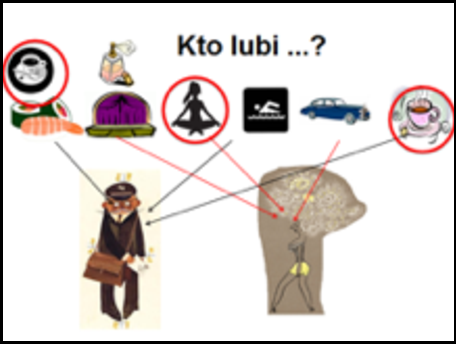
\includegraphics[width=\textwidth]{figures/02-1.pdf}
    \fbox{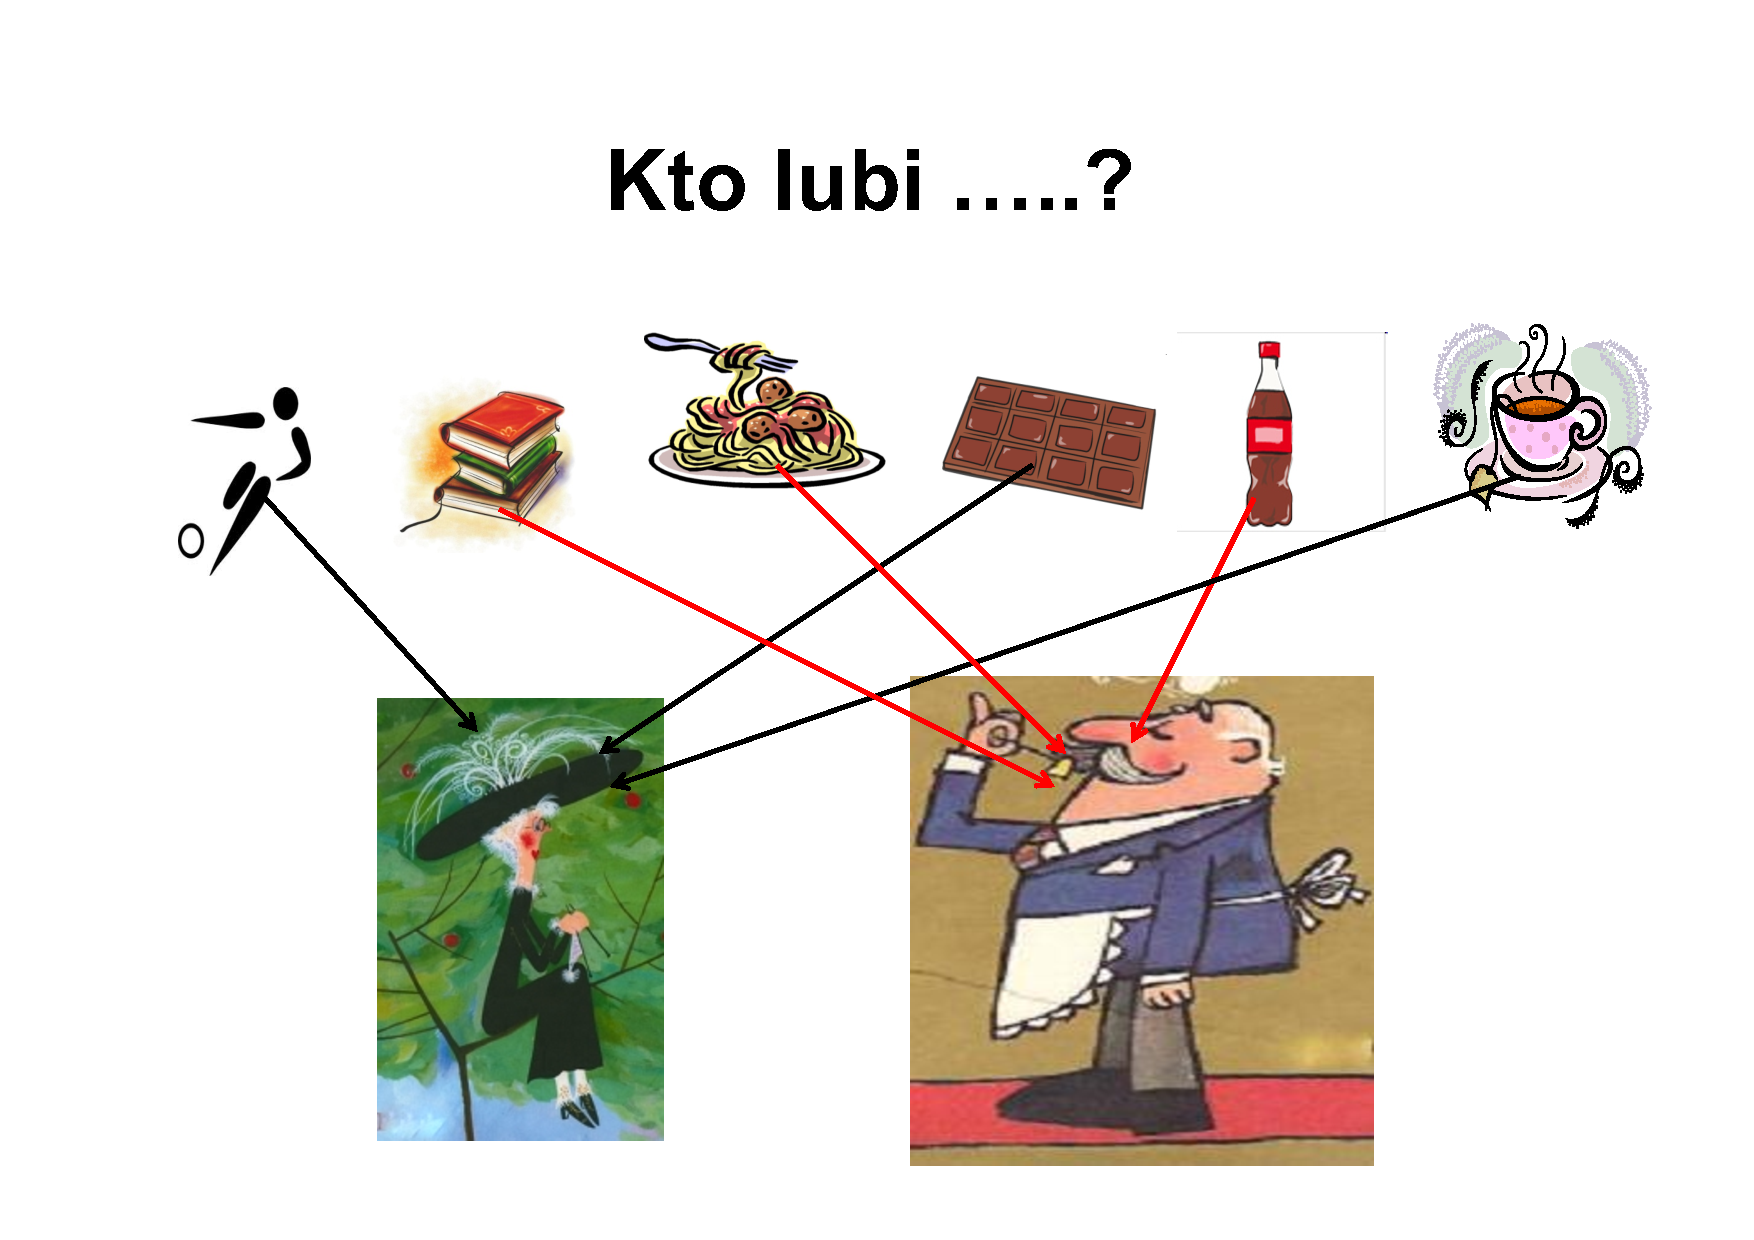
\includegraphics[height=.4\textheight]{figures/2-1.pdf}}
    \caption{MB input example slide}
    \label{fig:02:1}
\end{figure}

In contrast, the FB groups were exposed to enhanced input (\citealt{Sharwood-Smith1993}), designed to highlight specific formal features of the input. This was mainly achieved through focus-on-form activities (\citealt{DoughtyWilliams1998}) and corrective feedback. Linguistic information was visually presented in a more explicit fashion, as exemplified in \figref{fig:02:2}.

\begin{figure}[p]
    \fbox{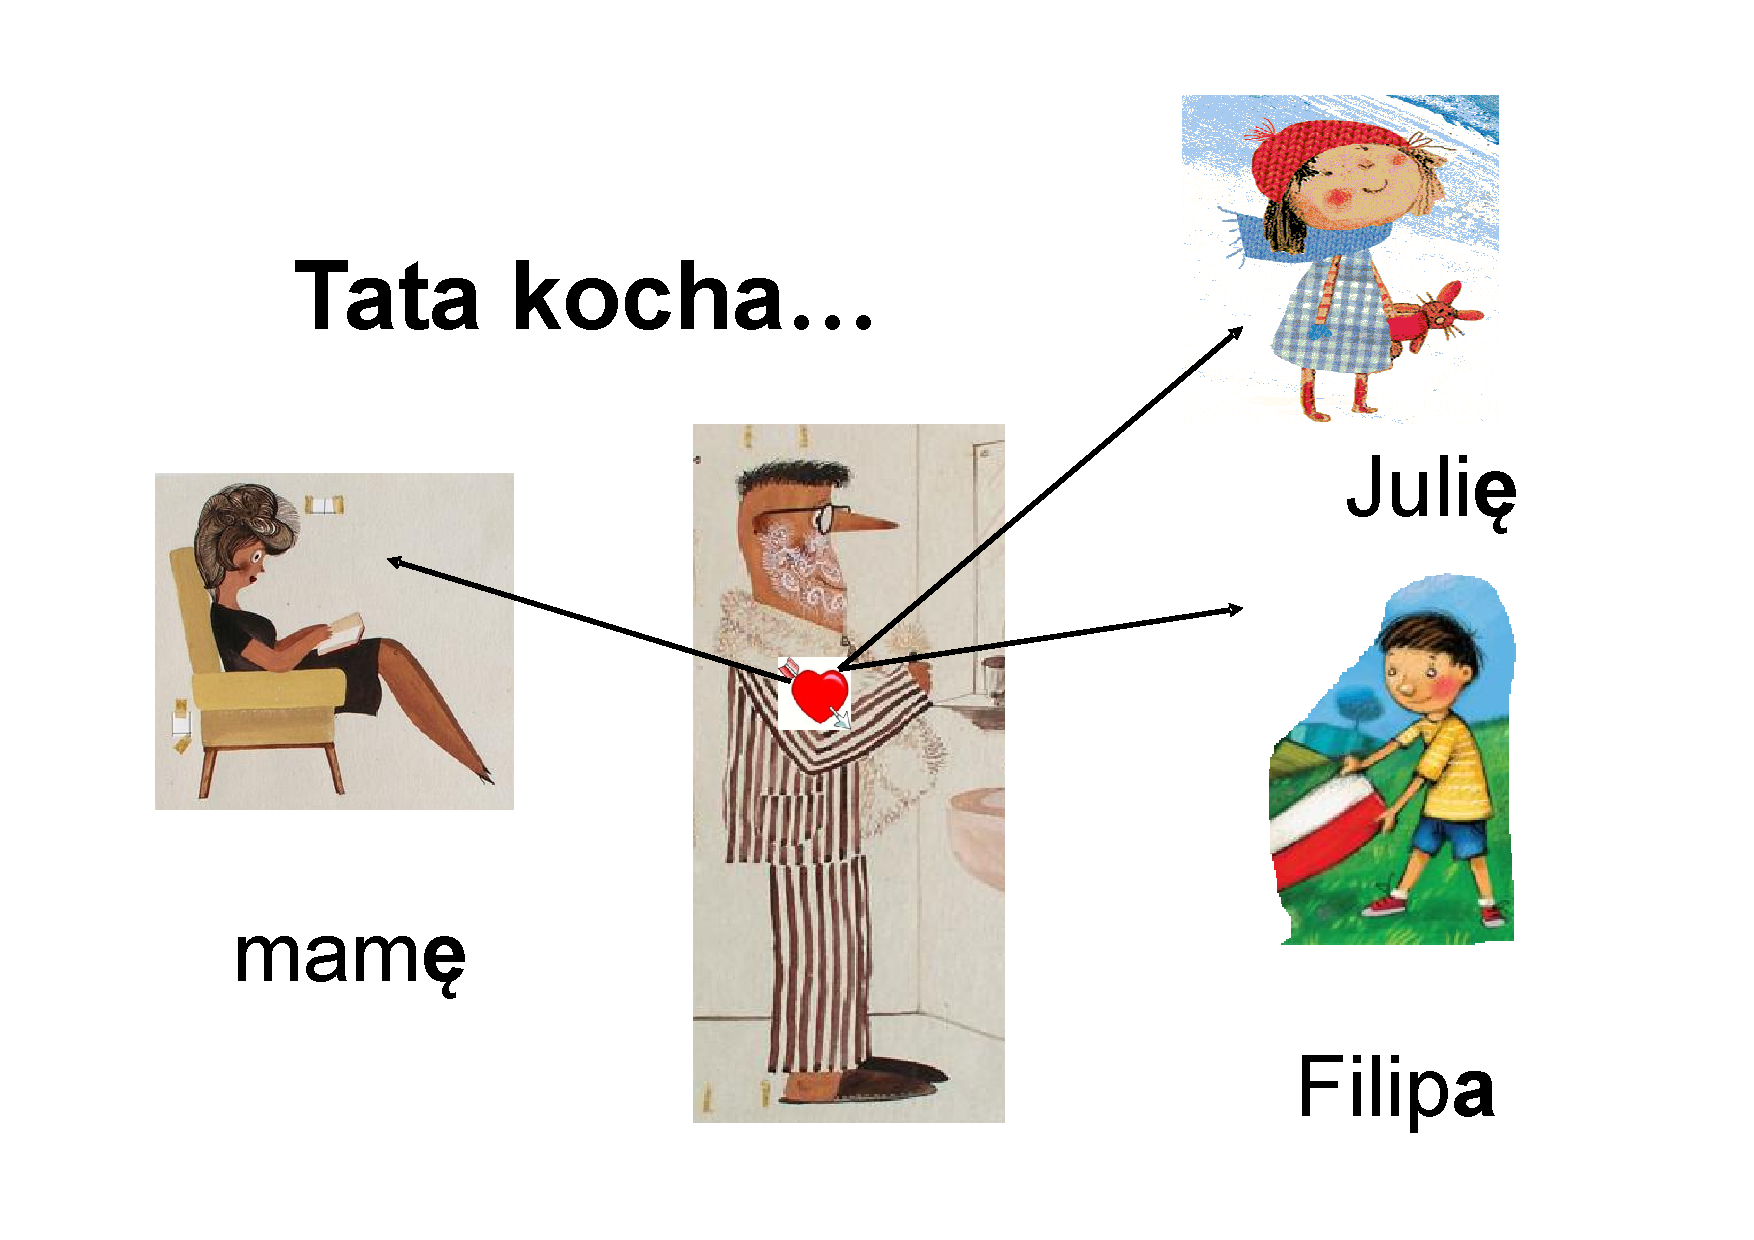
\includegraphics[height=.4\textheight]{figures/2-2.pdf}}
    \caption{FB input example slide}
    \label{fig:02:2}
\end{figure}

The written word-forms of target items (here, again, the accusative case) are presented on screen and graphically highlighted, e.g. the \textit{-ę} ending in bold, so that learners are provided with a set of meta-linguistic information. Just like its MB counterpart, however, the FB input includes no metalanguage, and students were never provided with explicit explanations as to the target grammar. 

Beside these differences, the input contents were the same for both groups. In addition to the range of lexical items and grammatical structures, their frequency and order of appearance in particular were kept as uniform as possible. 

\subsection{Input control}\label{sec:02:1.1}

As stated in the introduction, one of the major objectives of the VILLA project was a detailed, fine-grained analysis of the relation between input and intake. It is clear that thorough input control is an essential prerequisite in order to pursue this research question. In the VILLA project this ambitious objective required several steps.

First, one had to control for the participants’ existing experience of the target language. This was  only possible through the exclusion of participants who declared any previous contacts with Polish or other Slavic languages. Second, it was necessary to make sure that exposure to Polish throughout the course would be limited to the experimental input, including teacher speech and a set of PowerPoint slides. The choice of Polish as a target language made it rather unlikely that participants could accidentally be exposed to it outside classes. In any case, all participants signed a contract to the effect that they would not intentionally look for additional information on Polish. Clearly it is impossible to verify whether or not this requirement was respected.

In order to make the experimental input as uniform as possible in terms of both quantity and quality, learners were asked not to take notes during classes. The rationale behind this decision is that the quality of learners’ notes as well as their effort would very likely differ from person to person, thus introducing an undesirable variable beyond methodological control. For the same reason, no homework was assigned and individual practice outside classes was discouraged.

Finally, input was carefully planned in terms of topics, vocabulary and frequency of both lexical items and syntactic structures. This resulted in a general scheme which the teacher replicated with remarkable accuracy throughout the various editions of the course. Classes would never be identical to each other, as they were not recorded but performed live. Nevertheless, since frequency was one of the variables controlled for in the tests, it was vital that the target linguistic items should occur an equal number of times in each edition. To this aim, classes were monitored in real time by a team member, who signalled to the teacher whether a given word had appeared too rarely or too often in relation to its planned frequency. An \textit{a posteriori} analysis on the input corpus showed that lexical frequencies were indeed comparable across the editions of the VILLA project, which is a real credit to the teacher for managing to maintain consistency over ten different courses and a time span of almost a year.

\subsection{Input transcription}\label{sec:02:1.2}

By far the most thorough tool of input control was input recording and transcription, so that it can now be accessed and studied in a written format. The teacher wore a portable wireless microphone which recorded her speech. The resulting tracks were subsequently transcribed\footnote{The input for Italian and English editions was transcribed by Jacopo Saturno; the French, German and Dutch editions were  transcribed by members of the corresponding research teams.} in standard orthography using ELAN (\citealt{BrugmanRussell2004}). This software makes it possible to time-align transcriptions, i.e. to automatically associate each annotation with the corresponding audio segment (\figref{fig:02:3}). Transcription is produced from left to right along the horizontal axis; participants are assigned different tiers which are listed from top to bottom.

\begin{figure}
    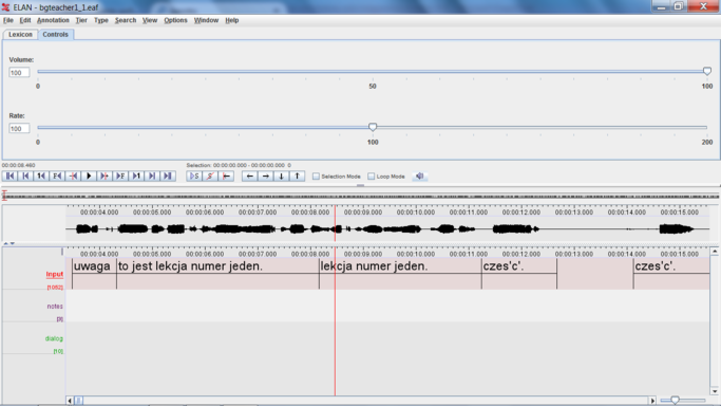
\includegraphics[width=\textwidth]{figures/02-3.pdf}
    \caption{transcription of the VILLA input with ELAN}
    \label{fig:02:3}
\end{figure}

To separate input addressed to all learners from comments aimed at individual learners or groups during interactional games, teacher speech was transcribed on two different tiers, labelled *TEA and *TEB respectively. Since it represents the vast majority of utterances, only the former is considered in this work. The ELAN files were converted into a vertically oriented text format using the CHAT/CLAN \citep{MacWhinney2000} suite of software (\tabref{tab:02:1}).

\begin{table}
\ttfamily
    \begin{tabular}{lrl}
        6    &   *TEA: & uwaga\\
        7    &   *TEA: & to jestlekcjanumerjeden . \\
        8    &   *TEA: & lekcjanumerjeden .  \\
        9    &   *TEA: & cześć .  \\
        10   &   *TEA: & cześć .  \\
        11   &   *TEA: & cześć .  \\
        12   &   *TEA: & cześć .  \\
        13   &   *TEA: & bardzodobrze .  \\
        14   &   *TEA: & cześć .  \\
        15   &   *TEA: & to jestkontaktnieoficjalny .  \\
        16   &   *TEA: & kontaktnieoficjalny .  \\
        17   &   *TEA: & cześć .  \\
        18   &   *TEA: & cześć . \\
    \end{tabular}
    \caption{transcription of the VILLA input in CHAT}
    \label{tab:02:1}
\end{table}

A CHAT-CLAN automatic morphological tagging system was developed by Christine Dimroth and Roman Skiba, with a small contribution by the present author (\tabref{tab:02:2}). 

\begin{table}
\ttfamily
    \begin{tabular}{ll}
        *TEA:   & uwaga\\
        \%mor:  & Noun|uwaga:Nom-fem-Sg=attention\\
        *TEA:   & to jestlekcjanumerjeden . \\
        \%mor:  & Pron|ten:demon-3-Sg-neutr-Nom=this Cop|być:3-Sg=be \\
        ~       & Noun|lekcja:Nom-fem-Sg=lessonNoun|numer:Nom-masc-Sg=number\\
        ~       & Num|jeden:cardinal=one . \\
        *TEA:   & lekcjanumerjeden .  \\
        \%mor:  & Noun|lekcja:Nom-fem-Sg=lessonNoun|numer:Nom-masc-Sg=number\\
        ~       & Num|jeden:cardinal=one . \\
        *TEA:   & cześć .  \\
        \%mor:  & Adv|cześć=bye-or-hello . \\
        *TEA:   & cześć .  \\
        \%mor:  & Adv|cześć=bye-or-hello . \\
    \end{tabular}
    \caption{automatic morphological tagging of the VILLA input in CHAT}
    \label{tab:02:2}
\end{table}

On the dependent tier \texttt{\%mor}, each word is morphologically tagged with the appropriate values of the relevant grammatical categories, depending on the word class considered (e.g. case, gender, number and lexeme for nouns; person, number and lexeme for verbs; and so on). To each item in the original transcript, the CLAN Mor programme associates the appropriate gloss, retrieving it from a specially designed lexicon. In case a given form corresponds to more than one tag, which because of widespread morphological syncretism is a fairly common case in Polish, all tags are presented subsequently. Glosses were not disambiguated in any way.

Building on that basis  a similar yet separate system was developed for the purposes of the present work by adapting the same principle to a different tool, namely the software R (\citealt{RCoreTeam2017}) and its package \textit{stringr} \citep{Wickham2017}. New labels (in Italian) were also devised for all grammatical categories, such as verbs, pronouns and adjectives. Compared to the system presented above, this new version facilitates frequency searches for morphosyntactic patterns in several technical respects.

Again, tags may include more than one possible grammatical meaning, as exemplified in \REF{ex:02:1}.

\ea%1
    \label{ex:02:1}
    \ttfamily\small
    \textit{balonik}:sostantivoIN\_Acc\_Mas\_Sg//sostantivoIN\_Nom\_Mas\_Sg:balonik
    \z

The input transcript, once glossed, can be searched for appropriate patterns through regular expressions. A search for SVO sentences with animate masculine nouns as subject and inanimate feminine nouns as object, for example, should retrieve hits like \textit{Leon lubi herbatę}, ‘Leon likes tea’. In addition, it is possible to identify all the instances of a given lexeme or grammatical value such as, for example, ‘nominative masculine singular’. 

\subsection{The VILLA input as a variety of Polish}\label{sec:02:1.3}

While the VILLA project uses a natural language as input, it would be imprecise to claim that the input provided by the teacher could be a representative example of native varieties. This is quite natural if one takes into account the peculiar context in which the experiment took place, including its time span, which was limited to 14 hours, and the research questions regarding the role of input, which could only be answered by manipulating it. These constraints result in a language variety which at times may sound a little odd to a native speaker of Polish. 

First, the dramatic competence gap between the teacher and the total beginner learners often results in a register definable as \textsc{teacher talk} (\citealt[134—144]{Larsen-FreemanLong1991}) whose purpose is to simplify the input as much as possible while maintaining grammatical correctness. In fact, teacher speech within the VILLA project was extremely slow and hyperarticulated in an effort to make input more salient, i.e. more easily perceivable and segmentable. 

Second, the choice was made to focus on a limited number of target structures, whose acquisition was later probed through the linguistic tasks. This caused them to be often produced with unnatural frequency, as is the case for the copula verb \textit{jest} ‘is’. Further, the frequency of syntactic structures directly conditions the frequency of the inflected word-forms belonging to the paradigm of a word. Compared to native varieties, input manipulation results in only a limited number of word-forms being represented in the VILLA input: plural forms for instance are completely absent for most nouns. Even within the singular number, the VILLA input is much more restricted than any L1 variety, being limited to only a couple of forms. Depending on the type of noun, the input might focus on the opposition between nominative and instrumental, for animate nouns, or between nominative and accusative, for inanimate ones. While most nouns only occurred in one or two forms, some did show a greater range of morphological endings. 

Copular structures usefully illustrate another source of deviations from native varieties, namely pragmatics. Two main types of predicational copular clauses may be distinguished in Polish \citep{Bondaruk2013}: In NOM-type structures (following the labels introduced in \citealt{Saturno2015}), the invariable pronoun \textit{to} ‘this’ is supplied independently of referent gender and number, while the complement appears in the nominative form, e.g. \textit{to jest Filip} ‘this is Filip’. INS-type structures, in contrast, require the personal pronoun \textit{on} ‘he’ or \textit{ona} ‘she’, which specify the gender of the corresponding referent, while the noun is provided in the instrumental case, e.g. \textit{on jest studentem} ‘he is a student’.

In native varieties of Polish, the two structures are pragmatically differentiated. NOM-type structures are mainly used deictically in order to introduce new referents in the discourse, e.g. \textit{a to, kto to jest?} ‘and this [person], who is this [person]?’. In contrast, the personal pronouns of INS-type structures typically refer to entities in an anaphoric manner, which means that the referent is already part of the discourse: the copular structure is used to provide additional details, e.g. \textit{kim on jest?} ‘who is he? [what's his job/nationality etc]?’ In contrast, in the VILLA input the two structures are used quite interchangeably in all contexts, so that no functional differentiation applies. Example \REF{ex:02:2}, extracted from the teacher's speech, shows that the two structures may be used to refer to the same entity in the same context. The teacher first asks (rhetorically) who Karol is using a an INS-type copular structure \REF{ex:02:2a}, which calls for the same structure in the responses in \REF{ex:02:2b} and \REF{ex:02:2c}. However, in \REF{ex:02:2d} the teacher switches to a NOM-type copular structure, in which the noun appears in the nominative case and the referent is deictically instantiated by the invariable pronoun \textit{to}, ‘this’. While this structure is grammatically correct, it would sound pragmatically inappropriate to a native speaker of Polish.

\ea%2
    \label{ex:02:2}
    \ea\label{ex:02:2a}
    \gll    A Karol, kim jest Karol?\\
            and Karol.\textsc{nom} who.\textsc{ins} is Karol.\textsc{nom}?\\
    \glt    ‘And Karol, who is Karol?’
    \ex\label{ex:02:2b}
    \gll    Karol jest stra\.{z}akiem.\\
            Karol.\textsc{nom} is fireman.\textsc{ins}\\
    \glt    ‘Karol is a fireman.’
    \ex\label{ex:02:2c}
    \gll    On jest stra\.{z}akiem.\\
            he is fireman.\textsc{ins}\\
    \glt    ‘He is a fireman.’
    \ex\label{ex:02:2d}
    \gll    To jest stra\.{z}ak.\\
            this is fireman.\textsc{nom}\\
    \glt    ‘This is a fireman.’
    \z
\z

Similar structures were produced intentionally for didactic purposes, i.e. in order to show learners that predications about referents may be expressed through different syntactic constructions. This contrast was also the target structure of several tasks. Most VILLA research questions are concerned with morphosyntax, which in light of the constraints imposed by a first exposure study necessarily led to a partial neglect of pragmatics and information structure. While this state of things seemed inevitable for methodological reasons, it has two negative consequences: first, as mentioned, the input at times might seem unnatural to a native speaker of Polish; second, the two contrasting structures end up to express exactly the same meaning, so that the contrast loses any functional motivation.

Similar arguments may be made concerning a crucial point of the present work, namely the order of subject and object in transitive sentences. Although both SO and OS orders are possible in Polish, this does not mean that different versions carry an identical meaning, at least from a pragmatic point of view \citep{Siewierska1993}. In general terms, the first position in the utterance is associated with the topic function, so that moving the object to that position from its canonical post-verbal position equals to treating the subject as the focus and the object as the topic. This is not necessarily the case in the VILLA project, as the input fragment in \REF{ex:02:3} makes clear.

\ea%3
    \label{ex:02:3}
    \ea\label{ex:02:3a}
    \gll    Filip wózek ciągnie.\\
            Filip.\textsc{nom} cart.\textsc{acc} pulls\\
    \glt    ‘Filip pulls the cart.’
    \ex\label{ex:02:3b}
    \gll    Filip ciągnie wózek tak.\\
            Filip.\textsc{nom} pulls cart.\textsc{acc} yes.\\
    \glt    ‘Filip pulls the cart.’
    \ex\label{ex:02:3c}
    \gll    Wózek ciągnie Filip.\\
            cart.\textsc{acc} pulls Filip.\textsc{nom}\\
    \glt    ‘Filip pulls the cart.’
    \z
\z

Compared to L1 practice, several facts are a little odd. First, the same referent is verbalised three times using maximally explicit means such as a person name. Second, based on the pragmatics of native Polish, one should conclude that \REF{ex:02:3a} focuses the verb, as in ‘Filip doesn't push the cart, he pulls it’; \REF{ex:02:3b}, at least in the absence of specific intonational patterns, should be interpreted as unmarked; in \REF{ex:02:3c}, finally, the focus would be on the subject, as in ‘it's not Julia who pulls the cart: it is Filip.' However, none of these interpretations is warranted in the example in question.

In fact, this obvious manipulation of syntax served the sole purpose of showing the learners that Polish word order is free. Unfortunately, given the very limited scope and vocabulary range of the VILLA project, at times it was impossible to do so in a pragmatically meaningful way, and the important link between information structure and syntax had to be sacrificed. On the one hand, word order manipulation was functional to research questions concerning cross-linguistic interference, such as “will speakers of rigidly SO languages be able to recognise and, perhaps, exploit Polish free word order?” On the other hand, it could be argued that the purpose of word order manipulation, i.e. the expression of pragmatically marked meaning, could not be adequately inferred from the examples provided. 

In spite of these small differences with native varieties, it would be inappropriate to state that the VILLA Polish differs significantly from native varieties, or that it is not a natural language. The VILLA input retains numerous idiosyncrasies which are likely to create difficulties to the learners, and at the same time resemble the difficulties often encountered in SLA. Alongside a few instances of \textit{pluralia tantum}, several nominal paradigms present a range of idiosyncrasies and specificities which may not be immediately easy for the learner to grasp, such as the animacy-based differential object marking found in the paradigm of masculine nouns (see next section). To summarise, the VILLA input represents a specific variety of Polish, which retains the complexities and idiosyncrasies of a natural language, although it does present a limited range of lexical and grammatical items as well as a few instances in which syntax and pragmatics were somewhat bent to the need of didactics.

\section{The target language and the VILLA L1S}\label{sec:02:2}
\subsection{Inflectional morphology}\label{sec:02:2.1}

In addition to its low availability outside the language classroom in the countries where the VILLA courses were held, Polish was chosen as the target language of the experiment because it typologically differs from the VILLA L1s in various respects. One key feature is its rich and complex system of nominal morphology, contrasting two numbers, three genders in the singular and two in the plural, and crucially, as many as seven cases. \tabref{tab:02:3a} shows the paradigms which appear in the VILLA input. Virtually all nouns appeared in the singular number only, so much so that plural forms may be considered exceptional (they are mainly limited to a few \textit{pluralia tantum}) and will not be considered in this volume.

\begin{table}
    \begin{tabular}{llllll}
\lsptoprule
         & \textsc{m anim} & \textsc{f anim} & \textsc{m inanim} & \textsc{f inanim} & \textsc{neu}\\
\midrule
        NOM & strażak & mam-a & balonik & kaw-a & biurk-o\\
        GEN & strażak-a & mam-y & balonik-u & kaw-y & biurk-a\\
        DAT & strażak-owi & mam-ie & balonik-owi & kaw-e & biurk-owi\\
        ACC & strażak-a & mam-ę & balonik & kaw-ę & biurk-o\\
        INS & strażak-iem & mam-ą & balonik-iem & kaw-ą & biurk-iem\\
        LOC & strażak-u & mam-ie & balonik-u & kaw-ie & biurk-u\\
        VOC & strażak-u & mam-o & balonik-u & kaw-o & biurk-o\\
        & ‘fireman’ & ‘grandmother’ & ‘balloon’ & ‘coffee’ & ‘desk’\\
\lspbottomrule
    \end{tabular}
    \caption{Polish nominal paradigm, singular}
    \label{tab:02:3a}
\end{table}

The selection of the ACC ending depends on the interaction of animacy and grammatical gender, defined by noun-adjective agreement and NOM ending. Animacy is not relevant in the case of neuter and feminine nouns (\ref{ex:02:4a} and \ref{ex:02:4b}), but it determines whether the ACC of masculine nouns is identical to the NOM in non-palatalized consonant, as for inanimate nouns \REF{ex:02:4c}, or, in the case of animate nouns \REF{ex:02:4d}, to the genitive in \textit{-a} \REF{ex:02:4e}.

\ea%4
    \label{ex:02:4}
    \ea\label{ex:02:4a}
    \gll    Jan-${\emptyset}$ lubi kaw-ę\\
            Jan-\textsc{nom}  likes    coffee-\textsc{acc}\\
    \ex\label{ex:02:4b}
    \gll    Jan-${\emptyset}$ kocha mam-ę\\
            Jan-\textsc{nom} loves sister-\textsc{acc}\\
    \ex\label{ex:02:4c}
    \gll    Jan-${\emptyset}$ ma balonik-${\emptyset}$\\
            Jan-\textsc{nom} has balloon-\textsc{acc}\\
    \ex\label{ex:02:4d}
    \gll    Jan-${\emptyset}$ zna strażak-a\\
            Jan-\textsc{nom} knows fireman-\textsc{acc}\\
    \ex\label{ex:02:4e}
    \gll    to jest samochód-${\emptyset}$ strażaka\\
            this.\textsc{nom}  is  car-\textsc{nom}  fireman.\textsc{gen}\\
    \z
\z

Syncretism may obscure the one-to-one pairing of form and function. Even in a subset of Polish as is represented in the VILLA input, the inflectional ending \textit{-a} expresses at least two types of grammatical meaning in the nominal domain, i.e. NOM.F and GEN/ACC.M (the latter for animate nouns only), in addition to the 3\textsc{sg} of some verbs (e.g. \textit{on zna} ‘he knows’). Whenever instances of such categories co-occur, they present the same ending \REF{ex:02:5}. It follows that in order to apply the morphosyntactic principle of utterance decoding, the listener needs to be aware of the grammatical gender of the nouns involved as well as their inflectional paradigm.

\ea%5
    \label{ex:02:5}
    \gll    siostr-a lubi brat-a\\
            sister-\textsc{nom}  likes  brother-\textsc{acc}\\
    \z

In terms of inflectional morphology, the VILLA L1 closest to Polish is certainly German. This is the only L1 to express case on nouns, while all others only distinguish case on some personal pronouns. However, case in German is mainly signalled on the determiner (completely absent in Polish), while the inflectional paradigm is characterised by diffused syncretism, whereby several functionally differentiated word-forms are formally identical (\tabref{tab:02:4a}). Indeed, it has been shown (\citealt{KempeMacWhinney1998, KempeMacWhinney1999} for Russian) that the Slavic case is a much better cue to the identification of the sentence agent than it is in German, for both native speakers and learners.

\begin{table}
    \begin{tabularx}{\textwidth}{lXll}
    \lsptoprule
        \multicolumn{1}{c}{} &  & M & F\\
    \midrule
        \multicolumn{1}{c}{SING} & NOM & der Feuerwehrmann & die Köchin\\
        & GEN & des Feuerwehrmann-s & der Köchin\\
         & DAT & dem Feuerwehrmann & der Köchen\\
         & ACC & den Feuerwehrmann & die Köchin\\
         \midrule
        \multicolumn{1}{c}{PLUR} & NOM & die Feuerwehrmänn-er & die Köchin-nen\\
        & GEN & der Feuerwehrmänn-er & der Köchin-nen\\
         & DAT & den Feuerwehrmänn-ern & den Köchin-nen\\
         & ACC & die Feuerwehrmänn-er & die Köchin-nen\\
        \multicolumn{1}{c}{} &  & ‘fireman’ & ‘cook(F) ‘\\
\lspbottomrule
    \end{tabularx}
    \caption{German nominal inflection}
    \label{tab:02:4a}
\end{table}

The four remaining L1s, namely Dutch (\tabref{tab:02:3b}), Italian (\tabref{tab:02:4b}), French (\tabref{tab:02:5}) and English (\tabref{tab:02:6}) lack case altogether as far as nouns are concerned. These only present two forms, corresponding to singular and plural.

\begin{table}
    \begin{tabularx}{\textwidth}{lXll}
    \lsptoprule
        \multicolumn{2}{c}{Singular} & \multicolumn{2}{c}{Plural}\\
    \midrule
        M & F & M & F\\
        \midrule
        de brandweerman & de kokkin & de brandweerman-nen & de kokkin-nen\\
        ‘the fireman’ & ‘the cook.\textsc{f}’ & ‘the firemen’ & ‘the cooks.\textsc{f}’\\
\lspbottomrule
    \end{tabularx}
    \caption{Dutch nominal inflection}
    \label{tab:02:3b}
\end{table}

\begin{table}
    \begin{tabularx}{\textwidth}{XX@{\hspace{1cm}}Xl}
    \lsptoprule
        \multicolumn{2}{c}{Singular} & \multicolumn{2}{c}{Plural}\\
    \midrule
        F & M & F & M\\
        \midrule
        il pompier-e & la cuoc-a & i pompier-i & le cuoch-e \\
        ‘the fireman’ & ‘the cook.\textsc{f}’ & ‘the firemen’ & ‘the cooks.\textsc{f}’\\
\lspbottomrule
    \end{tabularx}
    \caption{Italian nominal inflection}
    \label{tab:02:4b}
\end{table}

The cases of French and English are particularly extreme. Regarding the former, even the singular and plural forms of the majority of nouns are only distinguishable in the written variety, as they are completely homophonous in speech: the only morphological cue to number is the determiner (\tabref{tab:02:5}).

\begin{table}
    \begin{tabularx}{\textwidth}{XX@{\hspace{1cm}}Xl}
    \lsptoprule
        \multicolumn{2}{c}{Singular} & \multicolumn{2}{c}{Plural}\\
    \midrule
        M & F & M & F\\
        {le} {pompier} & {la} {cuisinière} & {les} {pompiers} & {les} {cuisinières}\\
        /lə p\~{ɔ}.pje/ & /la kɥi.zi.njɛʁ/ & /le p\~{ɔ}.pje/ & /le kɥi.zi.njɛʁ/\\
        ‘the fireman’ & ‘the cook.\textsc{f}’ & ‘the firemen’ & ‘the cooks.\textsc{f}’\\
\lspbottomrule
    \end{tabularx}
    \caption{French nominal inflection}
    \label{tab:02:5}
\end{table}

Gender is not morphologically encoded in English nouns, which only distinguish a singular and a plural form (\tabref{tab:02:6}). Even when a noun is characterised in terms of intrinsic sex, this category is only visible through anaphoric reference.

\begin{table}
    \begin{tabularx}{\textwidth}{lXll}
    \lsptoprule
        \multicolumn{2}{c}{Singular} & \multicolumn{2}{c}{Plural}\\
    \midrule
        {the} {fireman} & {the} {cook} & {the} {firemen} & {the} {cook-s}\\
\lspbottomrule
    \end{tabularx}
    \caption{English nominal inflection}
    \label{tab:02:6}
\end{table}


As far as word order is concerned, Polish is a predominantly SVO language \citep{rothstein_polish_2002, Dryer2013a}, although the encoding of case makes it possible to freely manipulate it for pragmatic purposes. Word order in German may also be manipulated for pragmatic reasons without the need for specific syntactic devices (such as cleft sentences), because syntactic functions are made explicit by case marking. It is worth noting that, unlike Polish, German word order is constrained by the obligatoriness of the finite verb in second position.

In all VILLA L1s except German, the lack of explicit case marking results in syntactic functions being assigned based on the default SO word order. In Italian, for instance, departures from this pattern \REF{ex:02:6a} are possible, but require marked phonological or syntactic means, particular intonational contours, cleft sentences \REF{ex:02:6b} or dislocations \REF{ex:02:6c}. Of course, all these possibilities are also available in languages with more complex morphology, like Polish \REF{ex:02:6d}. Word order manipulation in these languages is simply an extra resource to explicitly mark information structure \REF{ex:02:6e}, but this does not immediately translate into their being more flexible, or favouring more variable word orders. 

\ea%6
    \label{ex:02:6}
    \ea\label{ex:02:6a}
    \gll    il gatto insegue il cane\\
        \textsc{art.m.sg}  cat  chases \textsc{art.m.sg} dog\\
   \glt    ‛the cat chases the dog'\\
    \ex\label{ex:02:6b}
    \gll    è il gatto che insegue il cane\\
            is  \textsc{det.m.sg}  cat  \textsc{rel}  chases    \textsc{art.m.sg}  dog\\
\glt       ‛it is the cat that chases the dog'\\
    \ex\label{ex:02:6c}
    \gll    il cane lo insegue il gatto\\
            \textsc{art.m.sg}  dog  \textsc{pro.acc}  chases    \textsc{art.m.sg}  cat\\
   \glt    ‛it is the cat that chases the dog'\\
    \ex\label{ex:02:6d}
    \gll    to kot goni psa\\
            it  cat.\textsc{nom}  chases    dog.\textsc{acc}\\
     \glt    ‛it is the cat that chases the dog'\\
    \ex\label{ex:02:6e}
    \gll    psa goni kot\\
            dog.\textsc{acc}  chases    cat.\textsc{nom}\\
    \glt    ‛the cat chases the dog'\\
    \z
\z

Because of the lack of articles \citep{Dryer2013a}, however, word order manipulation in Slavic languages is one of the main means to express definiteness (\citealt{JacennikDryer1992, Siewierska1993}).

As far as the lexicon is concerned, although numerous words belonging to international lexicon may be found, most Polish vocabulary is of Slavic origin and therefore fairly opaque to the VILLA learners. Lexical stress is fixed on the penultimate syllable, with the partial exception of learned loanwords from Latin or Greek as well as elements to which clitics are attached (both virtually absent from the experimental input). Among the VILLA L1s such rigid pattern is only found in French, where the stress is fixed on the last syllable of the intonation unit \citep{FougeronSmith1993}. 

\section{The learners}\label{sec:02:3}

Choosing an “exotic” language is surely a necessary step to run a first exposure study, but equally important is to make sure that the learners never had any experience of it. To this purpose, candidates to the VILLA project were first asked to fill a questionnaire regarding their linguistic repertoire: anybody who had been exposed to Slavic languages was excluded at this stage. Whenever possible, learners who had studied languages in which case is expressed morphologically, such as Greek, Latin or even German were also excluded. The reason for this is that the ideal VILLA participant is a linguistically naïve speaker of any of the VILLA L1s, who (with the sole exclusion of German native speakers) should not be aware of what grammatical case is and how it works. The explicit study of some languages, in contrast, inevitably implies some familiarity with this category. This might result in learners with that kind of experience processing Polish morphosyntax not just based on the input provided during the course, but rather thanks to their previous language skills. Fulfilling this criterion was particularly difficult in Italy and Germany, as many secondary school students take at least a year of Latin (\tabref{tab:02:7}). 

\begin{table}
    \begin{tabularx}{.66\textwidth}{Xrrrrrr}
    \lsptoprule
         & \multicolumn{5}{c}{L1 group} & \\
        Latin & Fr & GE & IT & NL & UK & Total\\
    \midrule
        Y & 2 & 8 & 14 & {}- & 0 & 24\\
        N & 15 & 12 & 3 & {}- & 17 & 47\\
        NA & {}- & {}- & {}- & 20 & {}- & 20\\
    \lspbottomrule
    \end{tabularx}
    \caption{Distribution of Latin skills by L1}
    \label{tab:02:7}
\end{table}

The candidates who were selected based on their language profile further took a “language sensitivity test”, in which they heard sentences in Polish, Russian and Finnish, and were asked whether or not they thought the sentences were in Polish. This was done in order to exclude people whose “intuition” appeared to be too good and could thus bias the results of the experiment.

The selection process took place identically in the five countries which participated in the initiative. For each L1 group, \tabref{tab:02:8} reports the total number of learners who took part in the VILLA MB course as well as their distribution by sex and the group mean age. Because of occasionally missing data, slight discrepancies in the total number of participants considered in the analysis may occur throughout this book.

\begin{table}
    \begin{tabularx}{.66\textwidth}{Xrrrrrr}
    \lsptoprule
         & EN & FR & GE & IT & NL & Total\\
    \midrule
        n. & 17 & 17 & 20 & 17 & 20 & 91\\
        sex: F & 13 & 12 & 13 & 9 & 10 & 57\\
        sex: M & 4 & 5 & 7 & 8 & 10 & 34\\
        mean age & 22 & 23 & 24 & 22 & 21 & 22\\
    \lspbottomrule
    \end{tabularx}
    \caption{learners by L1, MB group}
    \label{tab:02:8}
\end{table}

The vast majority of the VILLA participants were university students enrolled in a variety of degrees. Students of foreign languages, linguistics and psychology were excluded in order to avoid any potential bias related to a greater familiarity with the study of languages or the rationale of psycholinguistics experiments.

\section{Learner data collection}\label{sec:02:4}
\largerpage
The present section lists and describes the tasks which were used in the VILLA project to elicit linguistic data, with a particular focus on the tools which will be discussed in this book.

The main tool to elicit L2 data is represented by structured tests, schematically listed in \tabref{tab:02:9}. Although the focus is clearly on morphosyntax, several other levels of language were targeted as well.

\begin{table}
    \begin{tabularx}{\textwidth}{ll}
    \lsptoprule
        Test & Target\\
    \midrule
        Phoneme Discrimination & phonology\\
        Word Recognition & phonology\\
        Lexical Decision & vocabulary\\
        Grammaticality Judgement I (NOM/INS) & morphosyntax\\
        Picture Production & morphosyntax\\
        Comprehension (NOM/ACC) & morphosyntax\\
        Elicited Imitation (NOM/ACC) & morphosyntax\\
        Grammaticality Judgement II (NOM/INS) & morphosyntax\\
        Written word order & syntax\\
        Cloze test (Pronouns) & pro-drop\\
        Route direction & free production: reference to space\\
        Finite story \citep{Dimroth2012} & free production: film retelling\\
    \lspbottomrule
    \end{tabularx}
    \caption{VILLA project, linguistic tasks}
    \label{tab:02:9}
\end{table}

This book considers the results of two of these tasks, i.e. the Elicited Imitation (EI) and the Comprehension tasks. Precious linguistic data may be also extracted from a few interactional moments which took place during classes, in which learners were asked solve a simple communicative task in pairs or small groups. Indeed, one such instance will be used a source of semi-spontaneous production data in \chapref{sec:7}.

In order to control for specific learner attitudes which may have an impact on the tests above, individual difference measures were also taken (\tabref{tab:02:10}). Although correlations of these measures with the results of the structured tests have been attempted within the VILLA project (\citealt{WatorekSaturno2016, SaturnoWatorekInPrep}), these tasks will not be considered in the present work. 

\begin{table}
\small
    \begin{tabularx}{\textwidth}{XX}
    \lsptoprule
        Variable & Test\\
    \midrule
        Language profile & Language background questionnaire during recruitment interview\\
        \\[-1em]
        Nonverbal intelligence & Raven’s Standard Progressive Matrices\\
        \\[-1em]
        Personality (Big Five) & NEO FFI\\
        \\[-1em]
        Memory span & Digit span task\\
        \\[-1em]
        Working memory span & Sequencing Task\\
        \\[-1em]
        Executive function (attention and inhibition) & Flanker task\\
        \\[-1em]
        Cognitive style: perceptual preference & Barsch Learning Styles Inventory\\
        \\[-1em]
        Learning style & ISALEM-97\\
        \\[-1em]
        Motivation & Adapted from Gardner (2004) Attitude \& motivation test battery\\
        \\[-1em]
        Metalinguistic awareness: grammatical inferencing & llama F test \citep{Meara2005}\\
        \\[-1em]
        Metacognitive: associative learning & llama B test \citep{Meara2005}\\
        \\[-1em]
        Phonological memory/ awareness & llama D test \citep{Meara2005}\\
    \lspbottomrule
    \end{tabularx}
    \caption{VILLA project, psychometric tests (adapted from \citealt[125]{DimrothEtAl2013})}
    \label{tab:02:10}
\end{table}

\subsection{Transcription of the production tasks}\label{sec:02:4.1}

Two of the sources of linguistic data described in this book, namely the EI test (\sectref{sec:02:4.3}) and semi-spontaneous production (\sectref{sec:02:4.5}), aimed to elicit oral production data from the learner. As these data needed to be made available in a written mode for further analysis, learner responses were digitally recorded and subsequently transcribed\footnote{Transcribers: Joanna Hinz (German corpus), Katarzina Loziczka (Dutch corpus), Jacopo Saturno (Italian, French and English corpora).} using a combination of the ELAN (\citealt{BrugmanRussell2004}) and CLAN \citep{MacWhinney2000} software. As explained in Chapter 1, in a first stage the production data were transcribed phonetically, using either IPA \citep{LandauEtAl1999} or SAMPA (\citealt{Wells1995, Wells1997}) phonetic alphabets. In preparation for analysis, the transcripts made by individual transcribers were then normalised to broad IPA. No effort was made to accurately transcribe a few subtle phonological contrasts of Polish phonology, such as that between the series of post-alveolar \{ʃ,ʒ,ʧ,ʤ\}\footnote{These sounds are sometimes referred to as retroflex consonants and accordingly transcribed as \{/ʂ, ʐ, t͡ʂ, d͡ʐ/\}, although it can be argued that the notion of ``retroflex'' is quite problematic and may correspond to different phonetic realisations across the languages of the world (\citealt{Hamann2002, Hamann2003, Hamann2004, Żygis2003, ŻygisHamann2003, PadgettŻygis2007, ŻygisPadgett2010}). Throughout this book the symbols \{ʃ,ʒ,ʧ,ʤ\} will be used for reasons of readability.} and pre-palatal \{ɕ,ʑ,ʨ,ʥ\} consonants, or that between the high front /i/ and the high central /ɨ/ vowels, because there are not relevant for morphological analysis. When lexical stress is not specified, it is assumed that it falls on the penultimate syllable.

The production of centralised vowels by some learners required particular attention, as such sounds make it impossible to link the learner-produced form to one of the possible target word-forms. A word pronounced by a learner as [ˈpiwkə] for instance may correspond to both target /ˈpiwka/ \textit{piłk-a} ‘ball-\textsc{nom.sg}’ and target /ˈpiwke/ \textit{piłk-ę} ‘ball-\textsc{acc.sg’}. For the present analysis target items in which the ending produced was not clearly identifiable as either -/a/ or -/e/ were discarded, which led to the exclusion of 334 items. The problem proved particularly severe in the case of the German data, in which 242 items were excluded, most probably because of transfer of the German phonological rule of word-final vowel centralisation. 

Translations of learner output are not provided because of the difficulty to univocally ascertain what the learner really meant. Similarly, the gloss only indicates the input word-form which is closer to learner output, with no assumption that the indicated form was indeed the intended meaning.

\subsection{Data analysis and visualisation}\label{sec:02:4.2}

The data were entered into a spreadsheet format either manually (comprehension task) or semi-automatically using the export tools of ELAN (EIT and semi-spontaneous production). Descriptive and inferential statistics were then computed using the software R, version 3.6.0 (\citealt{RCoreTeam2017}); generalised mixed linear models were fitted thanks to the package \textit{lme4}, version 1.1-21 \citep{BatesEtAl2015}, while \textit{stringr}, version 1.4.0 \citep{Wickham2017} proved essential for string manipulation. Figures were produced using the tools of base R as well as the packages \textit{wordcloud}, version 2.6 \citep{Fellows2014} and \textit{extrafont}, version 0.17 \citep{Chang2014}. 

\subsection{The Elicited Imitation Test (EIT)}\label{sec:02:4.3}

The VILLA EIT is a highly structured task which learners took on two occasions, namely after 9 hours of exposure to the input (T1) and after 13:30 hours (T2). It was administered individually on a computer screen; depending on the course edition, headphones or the integrated computer speakers were used. 

The task was structured as follows. First, learners heard a short Polish transitive sentence, e.g. \textit{dziewczynka ciągnie portugalkę}, ‘little girl-\textsc{nom} pulls Portuguese woman-\textsc{acc}’. Subsequently, participants were required to draw on a separate answer sheet a simple geometric figure (exemplified in \figref{fig:02:6}) which appeared on screen.

\begin{figure}
    
\includegraphics[height=.3\textheight]{figures/02-6.pdf}
    \caption{EI task, distractors}
    \label{fig:02:6}
\end{figure} 

This step was included in the task in order to inhibit the learners' phonological memory, so as to make sure that they could not simply repeat a string of sounds, but rather had to process the target sentence in order to retrieve its meaning. It should be noted here that the drawing task didn’t involve articulatory suppression that might have disrupted subvocal rehearsal. Finally, learners were asked to repeat the target sentence as accurately as possible. Learner performances were not timed and no explicit time pressure was exerted.

Target sentences were 9 syllables long and had the structure Noun — Verb — Noun. Throughout the test, the two nouns always appeared in association with each other. One of the two nouns was classified as transparent (T), i.e. intuitively translatable, with some approximation, in every L1 of the VILLA project: e.g. \textit{portugalka}, ‘Portuguese woman’. The other noun was coded as non-transparent (NT), i.e. was completely opaque as to its meaning, e.g. \textit{dziewczynka}, ‘little girl’. While lexical transparency will not be considered in the analysis of the L2 data, this factor has been addressed in other works related to the VILLA project (\citealt{HinzEtAl2013, Saturno2014, Rast2015}). 

The stimuli were digitally recorded by the same female speakers. They were uttered with a slow speech rate and neutral intonation, so as to avoid any potential hints as to the pragmatic interpretation of the sentence. 

\largerpage
Target nouns belonged to the paradigm of the feminine nouns in -\textit{a}.\footnote{Polish feminine nouns belong to two different inflectional classes, depending on whether their nominative ends in -/a/, like \textit{żaba}, ‘frog’, or in a consonant, like \textit{noc}, ‘night’. Only elements belonging to the former class are represented in the VILLA input.} Each appeared in both the NOM and ACC case, instantiated by the endings -[a] (\textlangle{a}\textrangle) and -[e] (<ę>) respectively. Target sentences also varied with respect to constituent order, which could assume the values SVO or OVS. Since only the relative order of subject (S) and object (O) is relevant to the present analysis, henceforth SVO and OVS will be referred to as SO and OS, respectively, unless explicitly stated otherwise.

To summarise, each pair of nouns appeared in four target sentences, which makes it possible to isolate the parameters of case ending, word order and lexical transparency (\tabref{tab:02:11}). As there were 4 pairs of target nouns, the test included a total of 16 target sentences.

\begin{table}
    \fittable{
    \begin{tabular}{lll}
    \lsptoprule
        ~ & SO & OS\\
    \midrule
        NT — T & {dziewczynk-a woła portugalk-ę} & {dziewczynk-ę woła portugalk-a}\\
        & little girl\textsc{{}-nom} calls portuguese woman\textsc{{}-acc} & little girl\textsc{{}-acc} calls portuguese woman\textsc{{}-nom}\\
        \tablevspace
        T — NT & {portugalk-a woła dziewczynk-ę} & {portugalk-ę woła dziewczynk-a}\\
        & portuguese woman\textsc{{}-nom} calls little girl\textsc{{}-acc} & portuguese woman\textsc{{}-acc} calls little girl\textsc{{}-nom}\\
    \lspbottomrule
    \end{tabular}
    }
    \caption{EI task, target sentences}
    \label{tab:02:11}
\end{table}

\largerpage

For the purposes of this study, target items are represented by each nominal ending taken in isolation, rather than by entire utterances. Each target item, therefore, may be described in terms of the three parameters “target ending” (-[a] vs. -[e]), “target sentence constituent order” (SO vs. OS) and “carrier word lexical transparency” (T vs. NT). An example is presented in \tabref{tab:02:12}.

\begin{table}[b]
    \begin{tabularx}{\textwidth}{llllll}
    \lsptoprule
         {Kuchark-} & {/e/} & {woła} &  {Brazylijk-} & {/a/} & \\
          cook & \textsc{acc} & call \textsc{3sg} &  Brazilian woman & \textsc{nom} & \\
        &  &  &  &  & \\
        & {}-/e/ &  &  & {}-/a/ & Target ending\\
        & OS &  &  & OS & Constituent order\\
        & NT &  &  & T & Lexical transparency\\
        \multicolumn{5}{c}{} & \\
        \multicolumn{5}{l}{‘the Brazilian woman calls the cook’} & \\
    \lspbottomrule
    \end{tabularx}
    \caption{EI task, parameters of obligatory occurrences}
    \label{tab:02:12}
\end{table}

The values of the three parameters just discussed may combine in eight possible contexts (\tabref{tab:02:13}).

\begin{table}
    \begin{tabularx}{\textwidth}{Xllllllll}
    \lsptoprule
        target ending & {}-/a/ & {}-/a/ & {}-/a/ & {}-/a/ & {}-/e/ & {}-/e/ & {}-/e/ & {}-/e/\\
        constituent order & SO & SO & OS & OS & SO & SO & OS & OS\\
        lexical transparency & T & NT & T & NT & T & NT & T & NT\\
    \lspbottomrule
    \end{tabularx}
    \caption{EI task, combinations of parameters}
    \label{tab:02:13}
\end{table}

The test also included 16 filler sentences in the form of copular clauses with the structure “NP (Neg) COP AP/PP”, e.g. \textit{Aleksander nie jest z Meksyku}, ‘Aleksander is not from Mexico’. Finally, three warm-up sentences were included in the task to make sure that all learners had correctly understood the procedure.

\subsubsection{Theoretical premises}

Unlike the Comprehension test and the spontaneous production task described later on in this chapter, the EIT requires a thorough discussion of its theoretical premises and underlying mechanisms. The reason for this is that although it clearly is a highly structured test, it is often used (and indeed, it is used in this volume) as an approximation of spontaneous speech. Also known as “sentence imitation” or “sentence repetition”, the EIT is a language assessment method whereby participants are asked to listen to a target sentence and repeat it as accurately as possible, usually after some distracting pause. The rationale underlying this procedure is effectively summarised by \citet[79]{Buck2001}:

\begin{quote} Sentence repetition tasks work through listening, they require more than just listening skills. [...] As the sentences get […] longer, it seems likely that chunking abilities and the ability to deal with reduced redundancy will begin to become more important and, as with dictation, these are closely related to general linguistic competence. [...] They are integrative tests in that they test the ability to use language rather than just knowing about it, but only as long as the segments actually challenge working memory capacity. And they do require speech production.\end{quote}

Said otherwise, test-takers can accurately repeat only the grammatical structures that are already part of their developing L2 grammar, here interpreted as the ability to identify “chunks” of language, which are stored in working memory not as mere strings of sounds, but as meaningful units which are subsequently re-encoded based on the present state of the interlanguage grammar. The task has been successfully used to investigate the implicit competence of a wide range of populations, including L1 and L2 learners (both literate and illiterate, the task being administered orally) as well as patients affected by speech pathologies (\citealt{MarinisArmon-Lotem2015, Armon-LotemMeir2016}). 

On the practical side, the EI task offers numerous advantages to both language scientists and, to some extent, language testers (\citealt[187—189]{BrownAbeywickrama2010}): it is relatively quick and easy to administer, requires little equipment, and offers full control over the target structure (\citealt{Van-Moere2012}). This last point is certainly appealing to linguists, as it makes it possible to study linguistic structures which would otherwise take hours of spontaneous speech to observe, with no guarantee that they will surface at all (\citealt{FerrariNuzzo2009, BettoniDi-Biase2015}). For instance, eliciting the OS structures on which the present work is based would imply waiting for the learner to spontaneously produce a structure which requires a certain degree of grammatical competence as well as the appropriate pragmatic context, in addition to the learner's intention to exploit it. In other words, even if test takers can be thought to be equipped with the required grammatical and pragmatic competence, there is no warranty that they will use it even in the appropriate context, simply because they are in control of their own speech. Things may be forced to a little extent, for instance by using tasks which make a specific structure particularly appropriate in a given context: for example, one could imagine a situation in which the object of a verb is topicalised in discourse, and therefore could appear in utterance-initial position, as in \REF{ex:02:7}: 

\ea%7
    \label{ex:02:7}
    \ea\label{ex:02:7a}
    \gll    Kto gotuje kolacj-ę?\\
            who.\textsc{\textsc{nom}}   cook   dinner-\textsc{acc}\\
    \glt    ‘who is cooking dinner?’
    \ex\label{ex:02:7b}
    \gll    Kolacj-ę gotuję ja.\\
            dinner-\textsc{acc}   cook  I.\textsc{nom}\\
    \glt    ‘I am cooking dinner.’
    \z
\z

But this is just one out of many possibilities available to the learners. Speakers might just emphasise the subject pronoun using intonation, thus maintaining the default SO word order, or indeed produce an elliptic answer like \textit{ja} ‘I (will)’. In sum, although (semi)spontaneous speech is undoubtedly the most authentic \citep{Lewkowicz2000} measure of learner competence, so much so that various scholars, like \citet{Krashen1981} or \citet{Pienemann1998}, have long advocated that research should exclusively, or at least primarily rely on data obtained using this elicitation approach, it certainly is less practical than other elicitation techniques.

The EIT is typically administered orally, ensuring that both the prompt and the repetition are produced at a rate close to that of spontaneous speech and, therefore, that only implicit competence can be accessed: test takers should not have the time to rely on explicit, declarative knowledge \citep{Ellis2005}. This is a very important argument for those advocating the appropriateness of this task for the evaluation of the actual interlanguage state \citep{Erlam2006}.

\subsubsection{Memory in the EI test}

Target sentence design is vital to ensure that test-takers cannot repeat target sentences \textit{verbatim}. By relying on working memory (\citealt{Baddeley1986, Baddeley2003}), in fact, it is usually possible to remember short strings of sounds for a handful of seconds and then repeat them with reasonable accuracy \citep{Sachs1967}, even without necessarily understanding their meaning. This is due to the phonological loop (\citealt{BaddeleyEtAl1998}), the device which makes it possible to mentally store and rehearse a chain of sounds for some time before it fades. While this mechanism is seen as crucial in language learning, it represents a serious methodological obstacle to the validity of EIT as a measure of implicit (i.e., automatized, non meta-linguistic) lexico-grammatical competence. A properly designed experimental protocol should inhibit this mechanism by engaging the test-taker in some distracting activity, preferably of a verbal nature: even some delay between the presentation of the stimuli and their repetition should block the exclusive reliance on phonological memory (\citealt{JuffsHarrington2011}). Advocates of the EI test argue that under these conditions participants can remember meaning and lexico-grammar, but not phonological forms, which have to be produced anew in repetition. The test becomes reconstructive in nature, as participants listen to targets, decode them, and then re-produce them on the basis of the current developmental stage of the interlanguage. Indeed, test-takers have been reported to systematically produce ungrammatical structures or, conversely, correct ungrammatical targets (\citealt{HamayanEtAl1977}; \citealt{MunnichEtAl1994}). \citet{Håkansson1989} states that up to a specific developmental stage, a three-year old Swedish child consistently reproduced a NEG-AUX structure instead of the target AUX-NEG structure of the L1. Such studies are interpreted as evidence that test-takers do not just repeat a string of sounds, but interpret and reproduce it “in their own way”, often betraying the influence of factors such as markedness (as in \citeauthor{Håkansson1989}’s study) or L1 transfer. In this perspective, the EI test makes it possible to investigate to what extent the learner is able to bypass the constraints which shape the developmental stages of language acquisition, such as for instance the first-noun principle. 

From another perspective, \citet[325--326]{Van-Moere2012} builds on \citegen[168]{Skehan1998} notion of “processing competence” to suggest that the EI test is particularly apt to measure an under-researched, but vital skill such as processing efficiency, defined as “the speed and accuracy with which a learner orally processes familiar language”, which in turn tends to “near effortless processing of language”, or automaticity (\citealt{DeKeyser2001}). Such position proposes a largely lexically-based view of language, whereby words tend to occur in meaningful chunks which the language user treats as a single unit (\citealt{PawleySyder1983, Ellis2001}) and indeed have been shown to be processed with greater efficiency by both native speakers and language learners (\citealt{ConklinSchmitt2008}). Within Construction Grammar (\citealt{GriesWulff2005, HoffmannTrousdale2013}) and usage-based approaches (\citealt{Tomasello2005, CadiernoEskildsen2015, TylerOrtega2016}), chunks correspond to “constructions”, “form-function mappings that are conventionalized as ways to express meanings in a speech community” (\citealt[38]{WulffEllis2018}), where meaning can vary greatly in its degree of abstraction \citep{Goldberg2006}. The parallel is sometimes stated explicitly: “constructions can be viewed as processing units or chunks — sequences of words (or morphemes) that have been used often enough to be accessed together” \citep[51]{Bybee2013}. Again, constructions are not seen as the product of rules, but as language units: “patterns are stored as constructions even if they are fully predictable as long as they occur with sufficient frequency” \citep[5]{Goldberg1995}.

Against this background, the EI test is seen as a measure of acquisition in that it measures the learner’s ability to repeat strings which are too long and complex to be stored in phonological memory, which is described as containing about seven unrelated words or digits \citep{Miller1956} or two seconds worth of speech \citep{Baddeley1986}. Effectively, it has been shown that test-takers perform much better when asked to repeat meaningful speech than non-words (\citealt{GathercoleBaddeley2004}). Other studies (\citealt[86]{Underhill1987}; \citealt[79]{Buck2001}) further showed that only the shortest targets can be processed as mere strings of sounds. Repetition of meaningful speech is only possible through chunking and processing for meaning \citep[9]{Radloff1991}.

\begin{quote}As people become more familiar with a second language and more confident in manipulating its syntax, they are more able to pack the chunks full of information; and the more they control the morphology the better they are able to organize within chunks of syntax; and the more vocabulary they know the better they are able to hold on to the meaning until they can repeat the sentence.”\end{quote}

As a result, “only test takers who have developed sufficient automaticity in processing linguistic information will perform successfully” (\citealt[332]{Van-Moere2012}). 

The importance of processing for meaning as opposed to form is also underlined by \citet{Erlam2006}, who argues for the reconstructive nature of the test and inserts a comprehension question as a pause to inhibit phonological memory. Her claim is based on \citegen{Sachs1967} research, who demonstrated that while the exact lexical and morphosyntactic shape of a target sentence is lost soon after hearing it, memory for its general meaning lasts much longer.

\subsubsection{Appropriateness of the EI test for language assessment}

Not all researchers would agree with the rationale just described, and the relation of the EIT with working memory is certainly complex. Many factors are thought to influence the engagement of working memory in the task, including, among others, the nature and length of the stimuli, the type of distractor, the target structure, the learner's proficiency level, and many more (see \citealt{Vinther2002} and \citealt{Erlam2006} for a review). For the present purposes, it is sufficient to say that some argue that the EIT has nothing to do with implicit linguistic competence, and only measures a learner's working memory capacity (\citealt{JessopEtAl2007}), whereas others claim that working memory is only marginally involved if at all (\citealt{OkuraLonsdale2012}).

A good example of this debate is the controversy between \citet{ZhangLantolf2015} and \citet{Pienemann2015}. Aiming to verify the Teachability Hypothesis \citep{Pienemann1984}, \citeauthor{ZhangLantolf2015} exposed four English L1 learners of Chinese L2 to specially designed input. Learners were shown not only to be able to process structures deemed to be too advanced for their interlanguage, but also to skip developmental stages, which is excluded by \citeauthor{Pienemann2015}’s Processability Theory. \citet{Pienemann2015} questioned Zhang and Lantolf's results on various grounds, including their claim that they used the same elicitation methods and emergence criteria utilized in PT-inspired research: “data obtained through EI cannot be compared one to one with spontaneous speech production data. In terms of language processing, the two types of data tap into different psycholinguistic mechanisms” \citep[139]{Pienemann2015}. Indeed, a study by \citet{PienemanEtAl2013} experimentally demonstrated that learners of L2 Swedish systematically show better performance in repetition than spontaneous production. One key objective of that study was to differentiate formulaic echoes of teacher utterances and creative L2 production. Spontaneously produced structures were expected to be strictly in line with the L2 implicational hierarchy, while structures produced by the teacher, but beyond the learners’ current developmental stage could only be repeated as unprocessed fixed formulas. To verify these hypotheses, learners with various L1 background were exposed to a 30-minute one-to-one Swedish L2 lesson, whose purpose was to provide them with favourable conditions to produce formulaic speech by repeating teacher utterances. Following the lesson, the informants took part in four communicative tasks, regrettably not described in the chapter, structured in such a way as to ensure the elicitation of sentences which had not been heard during the lesson, thus representing creative output; this in turn is defined as structures which are not copies of the previous utterance. The results show that learners were able to repeat V2 structures following teacher input, but could not produce them spontaneously. Instead, in the relevant context, namely adverb fronting, they only produced the ungrammatical *Adv-SVO structure, which suggests that they were not developmentally ready to process V2. These findings are interpreted as evidence that structures beyond the correct processability stage can indeed be repeated as formulaic items without being processed, hence Pienemann's scepticism with regard to the EIT. In their response, \citet{LantolfZhang2015} note that the method used to elicit repetition by \citet{PienemannEtAl2013} is quite different from the typical EIT. Specifically, learners were asked to repeat teacher utterances straight after a stimulus sentence has been presented, whereas in \citeauthor{LantolfZhang2015}'s study (\citeyear{LantolfZhang2015}) they first had to perform a comprehension task. This is a sensitive point, as the design of EI tasks has been shown to have a direct and macroscopic impact on the kind of data it can produce. 

The EIT was also criticised for its lack of authenticity by \citet{Chun2006}, who defines this construct as “the degree of correspondence of the characteristics of a given language test task to the features of a Target Language Use task” (\citealt[23]{BachmanPalmer2009}), i.e. to what extent the experimental task simulates a real communicative situation: “with task-based tests, the developers need to show that the content of the test tasks is representative of the demands of the corresponding task outside the test situation, and that the scoring reflects this” \citep[43]{Luoma2004}. A commercial version of the EI task, Ordinate Corporation’s PhonePass Spoken English Test—10 (now marketed as Versant by Pearson), is used as a test of a candidate’s proficiency in spoken English in a variety of contexts, from job interviews to academic exams. Apart from the fact that the test is administered over the phone, \citegen[301]{Chun2006} critique mainly targets two points. First, shorter target sentences may be repeated by parroting and do not necessarily test processing for meaning; quoting \citet[79]{Buck2001}, it is argued the task “might test no more than the ability to recognize and repeat sounds, and this may not require processing of the meaning at all. ... [This] clearly fails \citegen{Anderson1972} criteria for proof of comprehension”. Second, target sentences are completely unrelated to any discourse or setting, so that the task does not reproduce a realistic communicative situation: “my interpretation of the speech production needed in the real-life domain of school and work necessitates the ability to create and interpret discourse by relating utterances to their meanings and intentions as well as the setting. Even a parrot can be taught to repeat short sentences devoid of any meaning or context”. This critique does not seem to take into account the “comprehensive body of psycholinguistic research that shows that this task does engage linguistic processing resources, and breakdowns in repetition performance in language learners occur in predictable patterns (e.g., misplaced grammatical morphemes, lexical substitutions, etc.; \citealt{EllisEtAl2006, Radloff1991})” as indeed was pointed out by the test developers in their response (\citealt[163--164]{DowneyEtAl2008}). \citet[330]{Van-Moere2012} also claims that the EIT is “more communicatively authentic than many people realize”, citing in support a variety of arguments. First, speakers often tend to make their own speech similar to that of the interlocutor’s in terms of both vocabulary and grammar (\citealt[313]{Levinson1983}; \citealt[89]{BrownYule1983}), which also plays an important role in the management of the interaction \citep[52]{Tannen2007}. Further, it has been suggested that paying attention to the form of an interlocutor’s speech may be advantageous in psycholinguistic terms, as the speaker is able to recycle that form and focus on the intended meaning (\citealt{Swain1985}; \citealt{BygateEtAl2001}).

Similar heated exchanges of opinions indicate that the EIT often produces output which is interpretable in radically different ways. To minimise this risk, methodological rigour is essential.

Within the VILLA project, the issues summarised above were addressed as follows. First, all target sentences were of the same length (9 syllables). Second, each stimulus sentence was followed by a short distractor task, albeit of a non-verbal nature. Finally, learners' working memory store was controlled using \citegen[8--10]{Meara2005} Llama D test, in which learners heard a target sentence followed by a shorter string of sounds and were asked to decide whether or not the shorter string was comprised in the target sentence. The words used in the target sentences are based on the ‟names of flowers and natural objects in a British Columbia Indian language [...], synthesised using AT\&T Natural Voices (French)" \citep[8]{Meara2005}. It is thus highly unlikely that any VILLA learner should be able to process them for meaning.

The test is inspired by research by Service (\citet{Service1992, ServiceKohonen1995}) and \citeauthor{SpecialeEtAl2004} (2004), who argue that the ability to recognise repeated sound patterns may be beneficial for both word learning and the noticing of morphological variability. 

In the present work the Llama D test will be mainly considered as a linguistically motivated test of phonological memory. Its output will be used to search for a positive correlation between WM store and success in the EIT, whose theoretical premises will~be considered as validated only in the absence of said correlation. Indeed, if repetition accuracy were found to depend on WM store, it would be illegitimate to consider the EIT as a measure of morphosyntactic skills, rather than mere phonological memory.

\subsection{The comprehension test}\label{sec:02:4.4}

In the VILLA Comprehension test, learners heard short Polish transitive sentences and subsequently saw two pictures in which the same two referents (a man and a woman) play different thematic roles: the same referent has the role of agent in one picture and of patient in the other one (\figref{fig:02:7}).

\begin{figure}[b]
    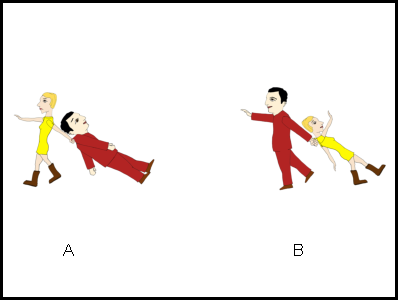
\includegraphics[width=\textwidth]{figures/02-7.pdf}
    \caption{Comprehension test: alternative descriptions of the target utterance}
    \label{fig:02:7}
\end{figure} 

The learners' task was to select the picture which in their opinion best depicted the stimulus sentence. Responses were marked in pen on an answer sheet. The data thus obtained were digitalised manually in spreadsheet format and then further manipulated and analysed with R (\citealt{RCoreTeam2017}).

\subsubsection{Comprehension test: target items}

The test comprises 24 target sentences, in addition to three warm-up sentences to make sure that learners had correctly understood its structure. The test was administered collectively in a classroom: target sentences were played aloud through loudspeakers while pictures were projected on screen. Learners took the test after 9 hours (T1) and 13:30 hours (T2) of exposure to the input, consistently with the timing of the EI test described in the preceding chapter: the two tasks probe different aspects of the learner's developing competence in the L2 after identical exposure to the input.

Target sentences had the structure NP — Verb — NP. Only two nouns were used for this test, namely \textit{brat}, ‘brother’, and \textit{siostra}, ‘sister’. The verbs were the same employed in the EIT, namely \textit{ciągnie}, ‘pulls’,  \textit{pcha}, ‘pushes’, \textit{pozdrawia}, ‘greets’, and \textit{woła}, ‘calls’. Each noun appeared in both its NOM and ACC form; further constituent order varied (SVO, OVS, OSV), each occurring in eight target sentences. 

\begin{table}
    \fittable{
    \begin{tabular}{l l@{~}l@{~}l@{\qquad}l@{~}l@{~}l}
    \lsptoprule
        \textit{siostr-a} & \textit{woła} & \textit{brat-a} & {~~~~~~} &        \textit{brat} & \textit{woła} & \textit{siostr-ę}\\
        sister-\textsc{nom} & calls & brother-\textsc{acc} & &        brother\textsc{.nom} & calls & sister\textsc{{}-acc}\\
        \tablevspace
        \textit{siostr-a} & \textit{brat-a} & \textit{woła} & &        \textit{siostr-ę} & \textit{brat} & \textit{woła}\\
        sister-\textsc{nom} & brother-\textsc{acc} & calls & &        sister-\textsc{acc} & brother\textsc{.nom} & calls\\
        \tablevspace
        \textit{brat-a} & \textit{woła} & \textit{siostr-a} & &        \textit{siostr-ę} & \textit{woła} & \textit{brat}\\
        brother-\textsc{acc} & calls & sister-\textsc{nom} & &        sister-\textsc{acc} & calls & brother.\textsc{nom}\\
    \lspbottomrule
    \end{tabular}
    }
    \caption{Comprehension test, example of target sentences with the verb \textit{woła}}
    \label{tab:02:14}
\end{table}

\tabref{tab:02:15} presents the relevant forms of the paradigm of the two target nouns employed in the test. \textit{Brat} follows the declension of masculine animate nouns, \textit{siostra} that of feminine nouns in -a.

\begin{table}
    \begin{tabularx}{\textwidth}{XXl}
    \lsptoprule
           & \textit{brat} ‘brother’ & \textit{siostra} ‘sister’\\
    \midrule
        NOM & \textit{brat} & \textit{siostr-a}\\
        ACC & \textit{brat-a} & \textit{siostr-ę}\\
    \lspbottomrule
    \end{tabularx}
    \caption{Comprehension test, paradigm of the target nouns}
    \label{tab:02:15}
\end{table}

As can be seen, the ACC case of masculine nouns like \textit{brat} is characterised by the ending \textit{{}-a}, which also occurs in the NOM case of feminine nouns like \textit{siostra}. This observation will be of some relevance in our subsequent analysis of the data.

\subsection{Semi-spontaneous production}\label{sec:02:4.5}

An essential part of the VILLA experimental protocol consists in the monitoring of learner output during classes. To this end, participants were seated in front of directional microphones which recorded everything they said during the whole course, as illustrated in \figref{fig:02:8}. The entire output of each participant was recorded on a separate track.

\begin{figure}
    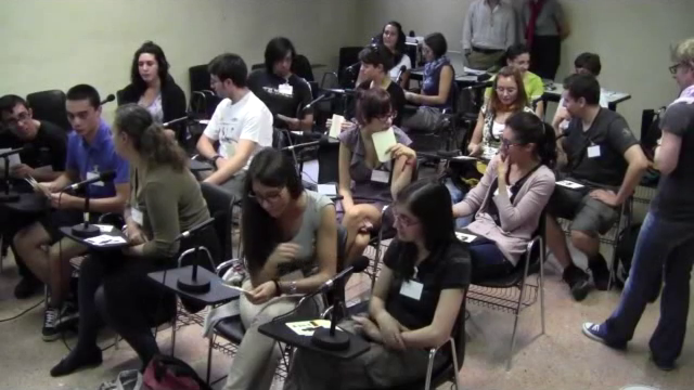
\includegraphics[width=\textwidth]{figures/02-8.pdf}
    \caption{VILLA classroom set-up}
    \label{fig:02:8}
\end{figure}

The VILLA course comprises several dialogic episodes during which participants could interact with each other. They were typically given a simple task to perform in pairs using grammatical structures or vocabulary which had been previously practiced collectively with the teacher. The data presented in this book were collected during one such occasion, which took place during lesson 7.2, after roughly 10:30 hours of exposure to the input. The development of the interlanguage at that stage should be roughly comparable to that probed though the structured tests (the EIT and the Comprehension test) at T1 (lesson 6.2, 9 hours of input exposure). Given the amount of work required to prepare the raw production data for analysis, only a subset of the VILLA dataset could be analysed, i.e. the Italian MB input group.

Participants were divided into 7 groups of 2 and a group of 3. Each group was given a set of cards containing information about several referents that learners were asked to describe to each other. Each card in a learner's set only contained part of the information: the remaining details could be found on the corresponding card in the partner's set, so that, in order to obtain a full description of the referent, information had to be exchanged between the two. While the first participant described the referent based on his or her card, the partner would try to identify the character, asking questions to complete the missing data. In doing so, learners were encouraged to use all structures presented during the course, including the transitive constructions which constitute the object of this work. 

For this study, the fragments relative to the interactive episode were extracted from the track of each participant and merged according to the groups in which learners were divided. Following this operation, each resulting track contained only the speech of the two or three participants who were part of the same group.  The data were then transcribed along the lines described in \sectref{sec:02:4.1} and further divided into one-verb utterances. Synchronised video recordings proved of great help to identify participants, providing the transcriber with an additional clue, in addition to the sound of learners' voices. The resulting corpus comprises 60 utterances produced by 17 learners.

\chapter{The Elicited Imitation Task}\label{sec:3}

\section{Research questions and hypotheses}\label{sec:04:1}

While a more detailed discussion of the theoretical premises of the Elicited Imitation test (EIT) was given in \chapref{sec:1}, it is worthwhile to repeat here that according to its rationale, the task does not require learners to simply repeat a string of sounds, but rather to decode its meaning and re-produce it ``in their own words'', i.e. based on the present state of their interlanguage grammar. In this respect, the task is used in this work as an approximation of a productive task. Unlike in free production tasks, however, EI makes it possible to maintain full control over the target structure, which seems particularly urgent in the case of rare, non-obligatory targets such as the OS structures investigated in this work.

The present chapter describes the structure of the VILLA EI task and presents the results obtained by the various L1 groups of the project. The analysis aims to identify the impact that independent variable: word order in target sentence, input, and L1 exert on dependent variable: accurate repetition of inflectional markers. Based on the information presented in the introduction, the following hypotheses may be formulated regarding the effect of the variables taken into consideration.

\begin{itemize}
    \item Word order: SO targets are expected to be processed with greater ease than the corresponding OS targets. This is due to the greater frequency of SO structures in the VILLA input as well as to their general unmarkedness from a pragmatic and typological point of view.
    \item L1: source languages in which case is expressed morphologically (such as German) should prove an advantage in the processing of a highly inflected L2 like Polish. Conversely, the rigid word order and lack of inflectional morphology of English and (spoken) French may slow down the acquisition process.
    \item Exposure to the input: greater length of exposure to the input (measured in hours) is expected to be beneficial to the development of the learners’ morphosyntactic skills.
\end{itemize}

Finally, an attempt will be made to correlate the results of the EI task with the Llama D test of implicit influence of pattern recognition ability on phonological memory, in order to verify whether or not the learners’ repetition performance is influence by this variable, whose involvement is typically excluded in the description of the rationale of the EI task.

\section{Results}\label{sec:04:2}

\subsection{Overview of learner output: overall repetition accuracy}\label{sec:04:2.1}

Overall repetition accuracy refers to the number of target segments which are correctly reproduced in a learner’s response. For the time being, the analysis will exclude inflectional endings, which will be treated in greater detail in the next sections. From a strictly phonological point of view, case endings such as [a] and [e] are segments like any other in the target string, and could therefore contribute to a measure of phonological accuracy. On the other hand, in the target language they are also inflectional morphemes conveying grammatical information. According to the assumptions of the EI task, the learner \textit{might} use them to derive and express syntactic functions, if the interlanguage has developed a morphosyntactic principle of utterance organisation: however, there are no \textit{a priori} means to establish whether that is the case or not. In short, it is hard to tell if the distribution of case endings is due to reasons pertaining to phonology (because the learner heard them that way) or morphosyntax (because the learner wanted to express a given syntactic function using the corresponding case ending).

Turning to an overview of phonological accuracy, most of the times lexical items appear to be fairly recognisable. Linguistic material may be omitted \REF{ex:04:1} or substituted \REF{ex:04:2}: compare the target in a. with learner output in b. 

\ea%1
    \label{ex:04:1}
    \ea\label{ex:04:1a}
    /ʤef'ʧink 'ʧongnie portu'galk/
    \ex\label{ex:04:1b}
    [ʤef'ʧink ʧon portu'galk]
    \z
\z

\ea%2
    \label{ex:04:2}
    \ea\label{ex:04:2a}
    /ʤef'ʧink 'ʧongnie portu'galk/
    \ex\label{ex:04:2b}
    [dy'ʧink 'bardzo portu'galk]
    \z
\z

In extreme cases, words may be mispronounced so badly that it is no longer possible to map them to existing word forms of the input, as [ʧyʒank] in \REF{ex:04:3}. At times, learner output appears to combine bits of two or more words from the input, as in \REF{ex:04:4}\footnote{See \citet{Saturno2015} for a discussion of similar examples and of the implications of transcription for all subsequent stages of data analysis.}, in which the item [unʧe'ʧelk] shows traces of the input words \textit{dziewczyna} [ʥefˈʧɨna] ‘girl’ and \textit{nauczycielka} [nauʧɨˈʨelka] ‘teacher’.

\ea%3
    \label{ex:04:3}
    /studentke pxa nauʧiʧelka/\\{}
    [ʧy'ʒank 'pxa unʧe'ʧelk]
    \z

\ea%4
    \label{ex:04:4}
    /portu'galk 'ʧongnie ʤefʧink/\\{}
    [portu'galk 'ʧoni ʧef'ʧelk]
    \z

\subsection{Overview of learner output: repetition of case endings}\label{sec:04:2.2}

The following transcripts present examples of correct \REF{ex:04:6} and incorrect \REF{ex:04:7} repetition of the case ending -[e] in identical target sentences, reported in \REF{ex:04:5}. Each sentence is followed by the speaker’s code and the time it was uttered. In incorrect repetitions both nouns are marked as -[a], on the model of the nominative case in the input, whereas in target-like output the two nouns are marked with different endings. Typically, each sentence presents either one or no errors.

\ea%5
    \label{ex:04:5}
    \ea\label{ex:04:5a}
    \gll    /artɨstk-e   pozdravja   twumatʃk-a/\\
            artist-\textsc{acc}  cheers    interpreter-\textsc{nom}\\
    \glt    ‘The interpreter cheers the artist.’
    \ex\label{ex:04:5b}
    \gll    /ʥevtʃɨŋk-a  ʨɔŋgnje   portugalk-e/\\
            little.girl-\textsc{nom}  pulls    Portuguese.woman-\textsc{acc}\\
    \glt    ‘The little girl pulls the Portuguese woman.’
    \ex\label{ex:04:5c}
    \gll    /brazɨlijk-a     vɔwa   kuxark-e/\\
            Brazilian.woman-\textsc{nom}  calls  cook-\textsc{acc}\\
    \glt    ‘The Brazilian woman calls the cook.’
    \z
\z

\ea%6
    \label{ex:04:6}
    \ea{\label{ex:04:6a}
    \gll    [artist-e  pɔzdravja   tumatʃk-a]\\
            artist-\textsc{acc}  cheers    interpreter-\textsc{nom}\\}\jambox*{(5104, T2)}
    \ex{\label{ex:04:6b}
    \gll    [dʒevtʃjenk-a  dʒɔnkje  portugalk-e]\\
            little.girl-\textsc{nom}  pulls    Portuguese.woman-\textsc{acc}\\}\jambox*{(5118, T1)}
    \ex{\label{ex:04:6c}
    \gll    [brazilik-a     vo'a   kurark-e]\\
            Brazilian.woman-\textsc{nom}  calls  cook-\textsc{acc}\\}\jambox*{(1119, T2)}
    \z
\z


\ea%7
    \label{ex:04:7}
    \ea{\label{ex:04:7a}
    \gll    [artistk-a   posdravja   tumatʃk-a]\\
            artist-\textsc{nom}  cheers    interpreter-\textsc{nom}\\}\jambox*{(2117, T2)}
    \ex{\label{ex:04:7b}
    \gll    [dʒevtʃinkn-a hm hm   portugalk-a]\\
            little.girl-\textsc{nom}  omission  Portuguese woman-\textsc{nom} \\}\jambox*{(4122, T1)}
    \ex{\label{ex:04:7c}
    \gll    [brazilik-a     wave   kukark-a]\\
            Brazilian woman-\textsc{nom}  calls  cook-\textsc{nom}\\}\jambox*{(3118, T1)}
    \z
\z

The same may happen with the repetition of -[a] NOM, although this is a much rarer event. The substitution of target -[a] with the competing ending -[e] produces a sentence in which both nouns are marked as -[e] (\REF{ex:04:8a}; target in \REF{ex:04:8b}).
\ea%8
    \label{ex:04:8}
    \ea{\label{ex:04:8a}
    \gll    [brazilijk-ɛ     vowa   vowa   kuxark-ɛ]\\
            Brazilian.woman-\textsc{acc}   calls   calls   cook-\textsc{acc}\\}\jambox*{(4113, T1)}
    \ex\label{ex:04:8b}
    \gll    /brazɨlijk-e     vɔwa     {} kuxark-a/\\
            Brazilian.woman-\textsc{acc}   calls     cook-\textsc{nom}\\
    \glt    ‘The cooks calls the Brazilian woman.’
    \z
\z
In rare instances, sentence with two errors may occur, in which case endings are swapped (\REF{ex:04:9a}; target in \REF{ex:04:9b}). 

\ea%9
    \label{ex:04:9}
    \ea{\label{ex:04:9a}
    \gll    [brazilijk-a     vowa   kuxark-e]\\
            Brazilian.woman-\textsc{nom}   calls   cook-\textsc{acc}\\}\jambox*{(2104, T1)}
    \glt    
    \ex\label{ex:04:9b}
    \gll    /brazɨlijk-e     vɔwa   kuxark-a/\\
            Brazilian.woman-\textsc{acc}   calls   cook-\textsc{nom}\\
    \glt    ‘The cook calls the Brazilian woman.’
    \z
\z

\subsection{Repetition of –[e]}\label{sec:04:2.3}

\subsubsection{Descriptive statistics}\label{sec:04:2.3.1}

The EI task was scored as follows: for each combination of time, word order and target ending, the scores of one or zero were assigned depending on whether or not the learner-produced output matched the expected target. The sum of these score was then divided by the number of targets produced (typically eight, but possibly less as a result of omissions or unrecognisable output, which were excluded from the analysis).

SO targets are generally processed with greater accuracy than OS ones, although scores remain rather low - below 50\% in most cases. Mean scores vary greatly across L1s, suggesting that there may be an important influence of the native language. Finally, variance is very high, which indicates that learners perform very differently from each other.

Information as to the performance of individual learners at T1 is presented graphically in \figref{fig:04:1}. In addition to standard boxplots, the individual data points are presented; their size is directly proportional to the number of learners achieving each score (also specified by the digits in white). Descriptive group statistics are provided in \tabref{tab:04:1}.

\begin{figure}
    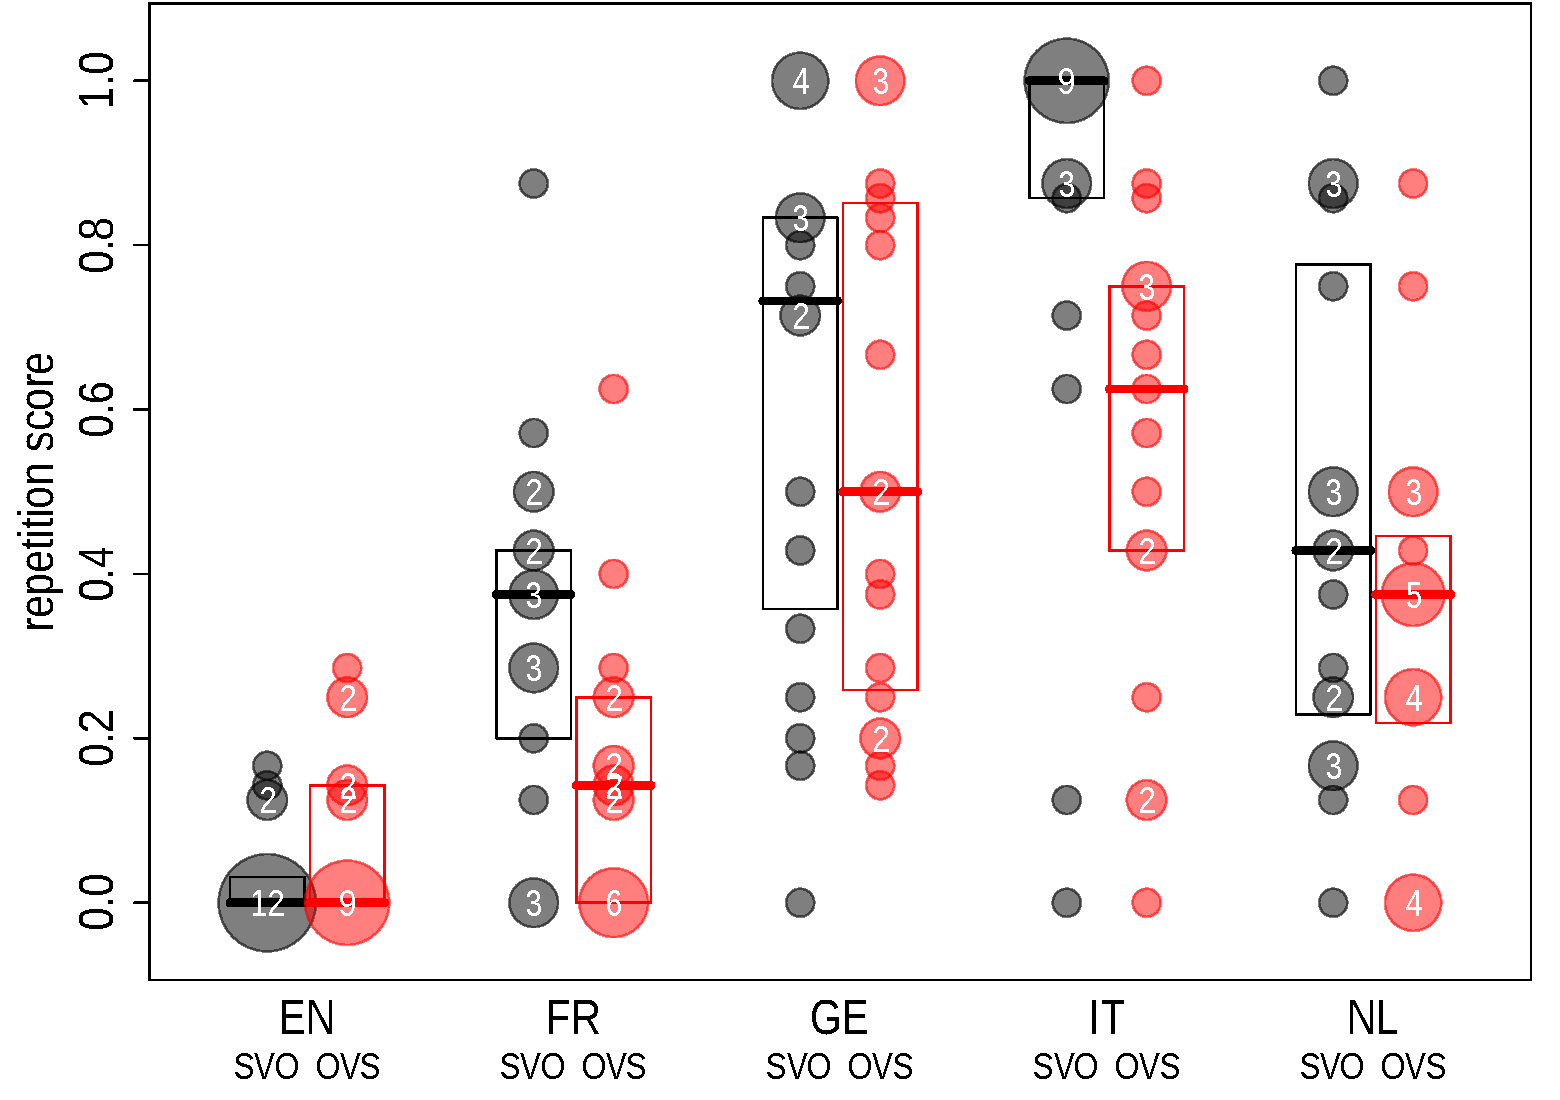
\includegraphics[width=\textwidth]{figures/04-1.pdf}
    \caption{EI task, [e] targets, T1, scores by L1}
    \label{fig:04:1}
\end{figure}

\begin{table}
    \begin{tabularx}{\textwidth}{XXXXXXX}
    \lsptoprule
    L1 & \multicolumn{3}{c}{ SO} & \multicolumn{3}{c}{ OS}\\
    & mean & sd & n & mean & sd & n\\
    \cmidrule{2-7}
    FR & 0.34 & 0.48 & 123 & 0.16 & 0.37 & 119\\
    GE & 0.62 & 0.49 & 82 & 0.57 & 0.50 & 110\\
    IT & 0.83 & 0.37 & 126 & 0.55 & 0.50 & 129\\
    NL & 0.48 & 0.50 & 147 & 0.33 & 0.47 & 155\\
    EN & 0.04 & 0.19 & 108 & 0.09 & 0.29 & 112\\
    \lspbottomrule
    \end{tabularx}
    \caption{EI task L1 descriptive statistics, -[e] ending, SO targets, T1}
    \label{tab:04:1}
    \label{tab:03:1}
\end{table}

The English L1 group consistently exhibits the poorest results, with most learners scoring exactly 0\%. No learner in this group ever scored over about 30\%. In contrast, the Italian group has the highest scores, followed by the German group and by the Dutch and French, somewhat behind. In all groups except the English and the French, at least one learner managed to reach 100\% accuracy. 

Individual variability within the L1 groups is extremely high, with learners’ scores ranging from 0\% to 100\%. The only exception, again, is the English group, in which scores are consistently close to floor level.

The picture looks fairly similar at T2 (\figref{fig:04:2} and \tabref{tab:04:2}), although a general improvement can be observed in the data.

\begin{figure}
    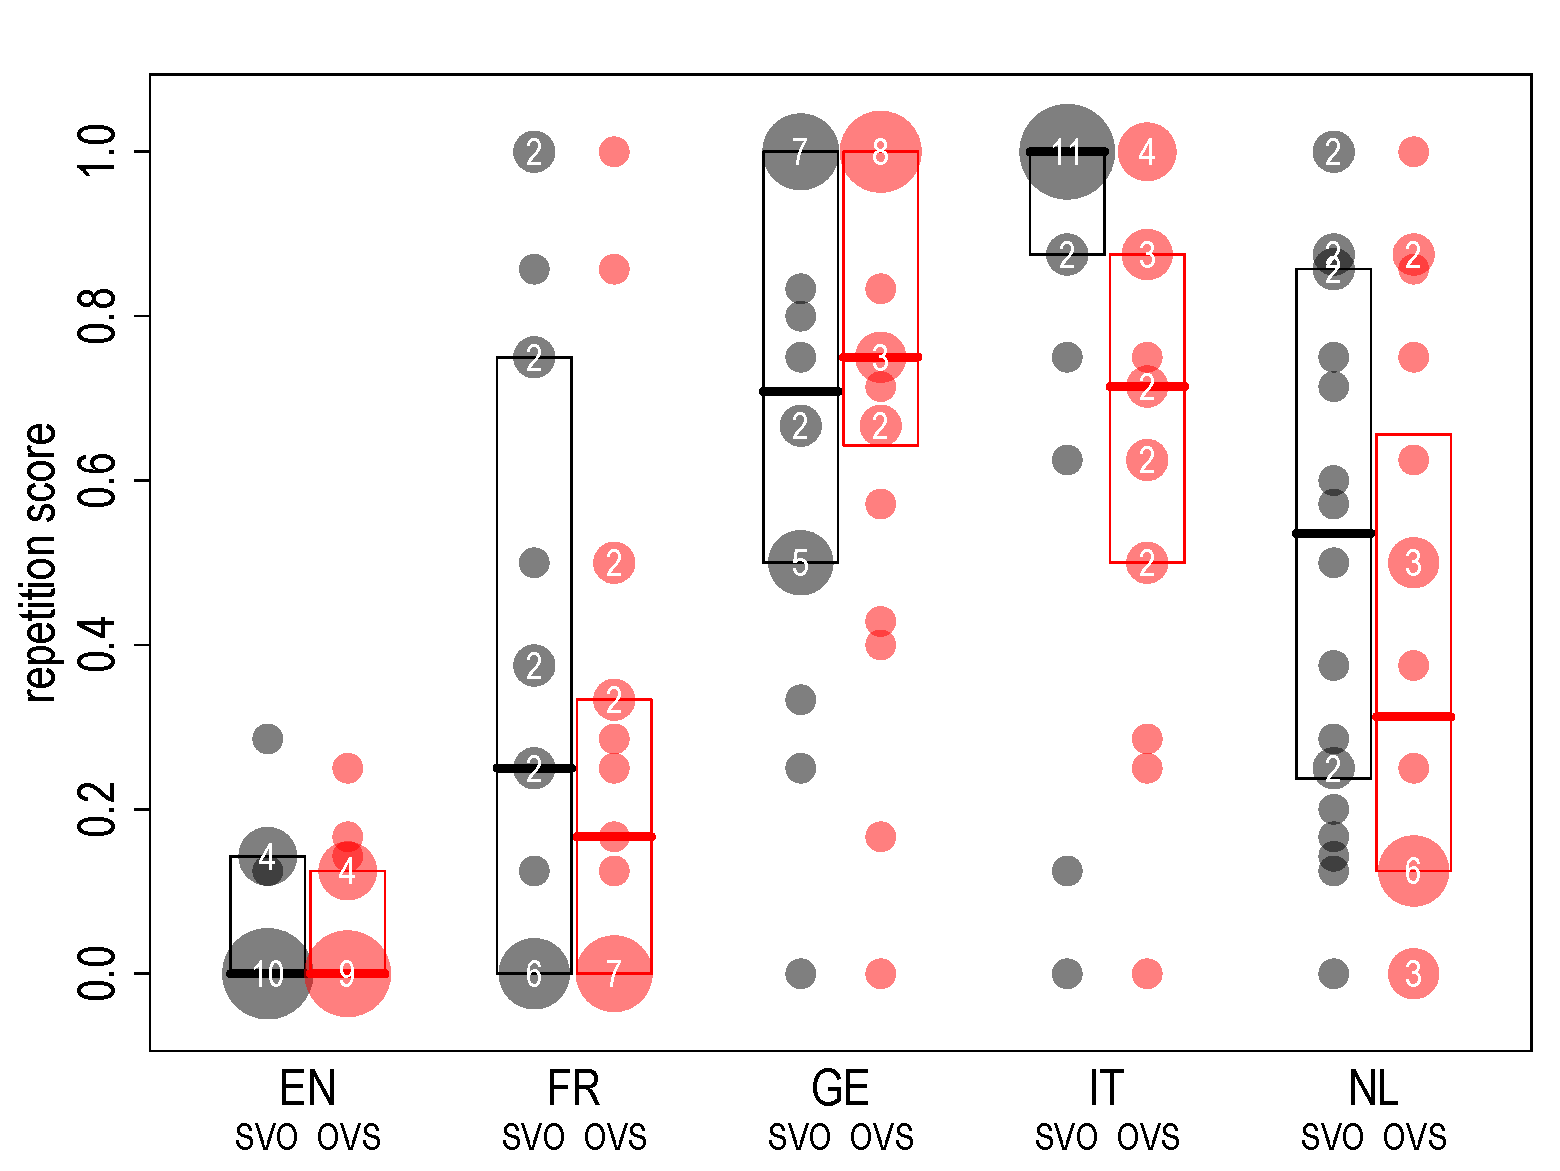
\includegraphics[width=\textwidth]{figures/04-2.pdf}
    \caption{EI task, [e] targets, T2, scores by L1}
    \label{fig:04:2}
\end{figure}

\begin{table}
    \begin{tabular}{lrrr rrr}
    \lsptoprule
    L1 & \multicolumn{3}{c}{ SO} & \multicolumn{3}{c}{ OS}\\
    & mean & sd & n & mean & sd & n\\
    \cmidrule(r){2-4}\cmidrule(l){5-7}
    FR & 0.39 & 0.49 & 126 & 0.26 & 0.44 & 121\\
    GE & 0.69 & 0.46 & 72 & 0.74 & 0.44 & 111\\
    IT & 0.87 & 0.34 & 127 & 0.69 & 0.47 & 131\\
    NL & 0.53 & 0.50 & 146 & 0.39 & 0.49 & 157\\
    EN & 0.06 & 0.24 & 118 & 0.07 & 0.25 & 118\\
    \lspbottomrule
    \end{tabular}
    \caption{EI task descriptive statistics, -[e] ending, OS targets}
    \label{tab:04:2}
    \label{tab:03:2}
\end{table}

\subsubsection{Inferential statistics}\label{sec:04:2.3.2}

A generalised linear mixed model \citep{Baayen2008} with binomial error structure and logit link function (Likelihood Type 3-test) was fitted to the data. Fixed effects comprised the L1 (five levels, reference level = EN), word order (binary, reference level = OS) and time (binary, reference level = T1) and the Llama test score (continuous, 0 to 1) as linear predictors, as well as the following two-way interactions: L1:word order, L1:time, and time:word order. Random effects included random intercepts for target sentence and participants as well as within-subject uncorrelated random slopes for time and word order. 

The rationale for including the interactions was as follows. The learners' ability to correctly repeat -[e] may be influenced by the word order of the target sentence, with SO targets generally facilitating correct repetition, and OS targets hindering it. In turn, the extent of this word order effect may be variably influenced by the learner’s L1. Further exposure is thought to be generally beneficial to repetition, but the extent to which results improve between T1 and T2 may be also determined by the learners’ L1: speakers of certain languages may improve more markedly than speakers of other languages. The effect of time is also likely to be constrained by word order. 

The summary of the model is presented in \tabref{tab:04:3}.

\begin{table}
    \begin{tabularx}{\textwidth}{Xrrr}
    \lsptoprule
    \textbf{~} & \multicolumn{3}{c}{ \textbf{response}}\\
    \textit{Predictors} & \textit{Odds} \textit{Ratios} & \textit{CI} & \textit{p}\\
    \midrule
    (Intercept) & 0.02 & 0.01~–~0.10 & \textbf{<0.001}\\
    time [2] & 0.76 & 0.22~–~2.62 & 0.661\\
    L1 [FR] & 2.79 & 0.85~–~9.19 & 0.091\\
    L1 [GE] & 38.27 & 11.65~–~125.66 & \textbf{<0.001}\\
    L1 [IT] & 15.27 & 3.96~–~58.84 & \textbf{<0.001}\\
    L1 [NL] & 9.70 & 3.01~–~31.24 & \textbf{<0.001}\\
    WO2 [SO] & 0.45 & 0.12~–~1.64 & 0.225\\
    llama & 4.57 & 0.71~–~29.39 & 0.110\\
    time [2] * L1 [FR] & 1.71 & 0.37~–~7.88 & 0.491\\
    time [2] * L1 [GE] & 2.97 & 0.65~–~13.68 & 0.161\\
    time [2] * L1 [IT] & 3.31 & 0.70~–~15.75 & 0.132\\
    time [2] * L1 [NL] & 1.96 & 0.46~–~8.38 & 0.362\\
    time [2] * WO2 [SO] & 0.93 & 0.57~–~1.53 & 0.775\\
    L1 [FR] * WO2 [SO] & 6.17 & 2.22~–~17.19 & \textbf{<0.001}\\
    L1 [GE] * WO2 [SO] & 3.13 & 1.06~–~9.30 & \textbf{0.040}\\
    L1 [IT] * WO2 [SO] & 19.50 & 6.26~–~60.74 & \textbf{<0.001}\\
    L1 [NL] * WO2 [SO] & 5.17 & 1.95~–~13.74 & \textbf{0.001}\\
    \multicolumn{4}{c}{\textbf{Random} \textbf{Effects}}\\
    σ\textsuperscript{2} & \multicolumn{3}{c}{3.29}\\
    τ\textsubscript{00}~\textsubscript{participant} & \multicolumn{3}{c}{1.41}\\
    τ\textsubscript{00}~\textsubscript{target\_no} & \multicolumn{3}{c}{0.87}\\
    τ\textsubscript{11}~\textsubscript{participant.WO2SO} & \multicolumn{3}{c}{2.19}\\
    τ\textsubscript{11}~\textsubscript{participant.time2} & \multicolumn{3}{c}{2.37}\\
    ρ\textsubscript{01}~\textsubscript{participant.WO2SO} & \multicolumn{3}{c}{1.00}\\
    ρ\textsubscript{01}~\textsubscript{participant.time2} & \multicolumn{3}{c}{{}-0.14}\\
    N~\textsubscript{participant} & \multicolumn{3}{c}{90}\\
    N~\textsubscript{target\_no} & \multicolumn{3}{c}{16}\\
    \midrule
    Observations & \multicolumn{3}{c}{2438}\\
    Marginal R\textsuperscript{2}~/ Conditional R\textsuperscript{2} & \multicolumn{3}{c}{0.550 / NA}\\
    \lspbottomrule
    \end{tabularx}
    \caption{Model summary}
    \label{tab:04:3}
\end{table}

The Llama score does not appear to be a significant predictor, which suggests that sensitivity to phonological patterns is not involved in determining success at the EIT. The three hypothesised interactions were explored by comparing the full model described above to three null models, each lacking the single interaction of interest. Statistical significance was assessed based on likelihood ratio tests: P values were corrected for multiple comparison using the Holm correction. The results are presented in \tabref{tab:04:4}.

\begin{table}
    \begin{tabularx}{.8\textwidth}{Xrrr}
    \lsptoprule
    predictor & Chisq & Chi Df & p\\
    \midrule
    time :L1 & 3.023 & 4 & > 0.05\\
    time : word order & 0.812 & 1 & > 0.05\\
    L1 : word order & 32.607 & 4 & < 0.01\\
    \lspbottomrule
    \end{tabularx}
    \caption{Full/null model comparisons}
    \label{tab:04:4}
\end{table}

Only the interaction involving L1 and word order proved to be statistically significant, which indicates that the impact of word order (SO vs. OS) varies based on the learner’s L1. 

The significant interaction was subsequently explored through pairwise comparison. The results relative to the role of the L1 are presented in \figref{fig:04:3}, in which blue bars represent confidence intervals for least square means. Pairwise comparisons are statistically significant if the red arrows do not overlap. Statistically significant contrasts are presented in \tabref{tab:04:5}.

\begin{table}
    \begin{tabularx}{\textwidth}{lQ}
    \lsptoprule
    Condition & pairwise comparison\\
    \midrule
    T1 OS & EN < GE (p < 0.01), IT (p <.01), NL (p < 0.01);\newline
    FR < GE (p <0 .01), IT (p < 0.01)\newline
    NL < GE (p = 0.04)\\
    \tablevspace
    T1 SO & EN < FR (p < 0.01), GE (p < 0.01), IT (p <.01), NL (p < 0.01)\newline
    FR < GE (p = 0 .01), IT (p < 0.01)\\
    \tablevspace
    T2 OS & EN < GE (p < 0.01), IT (p <.01), NL (p < 0.01);\newline
    FR < GE (p <0 .01), IT (p < 0.04)\\
    \tablevspace
    T2 SO & EN < FR (p < 0.01), GE (p < 0.01), IT (p <.01), NL (p < 0.01)\newline
    FR < GE (p < 0 .01), IT (p < 0.01)\\
    \lspbottomrule
    \end{tabularx}
    \caption{Pairwise comparisons, L1 : word order interaction (only significant contrasts shown)}
    \label{tab:04:5}
\end{table}

\begin{figure}
    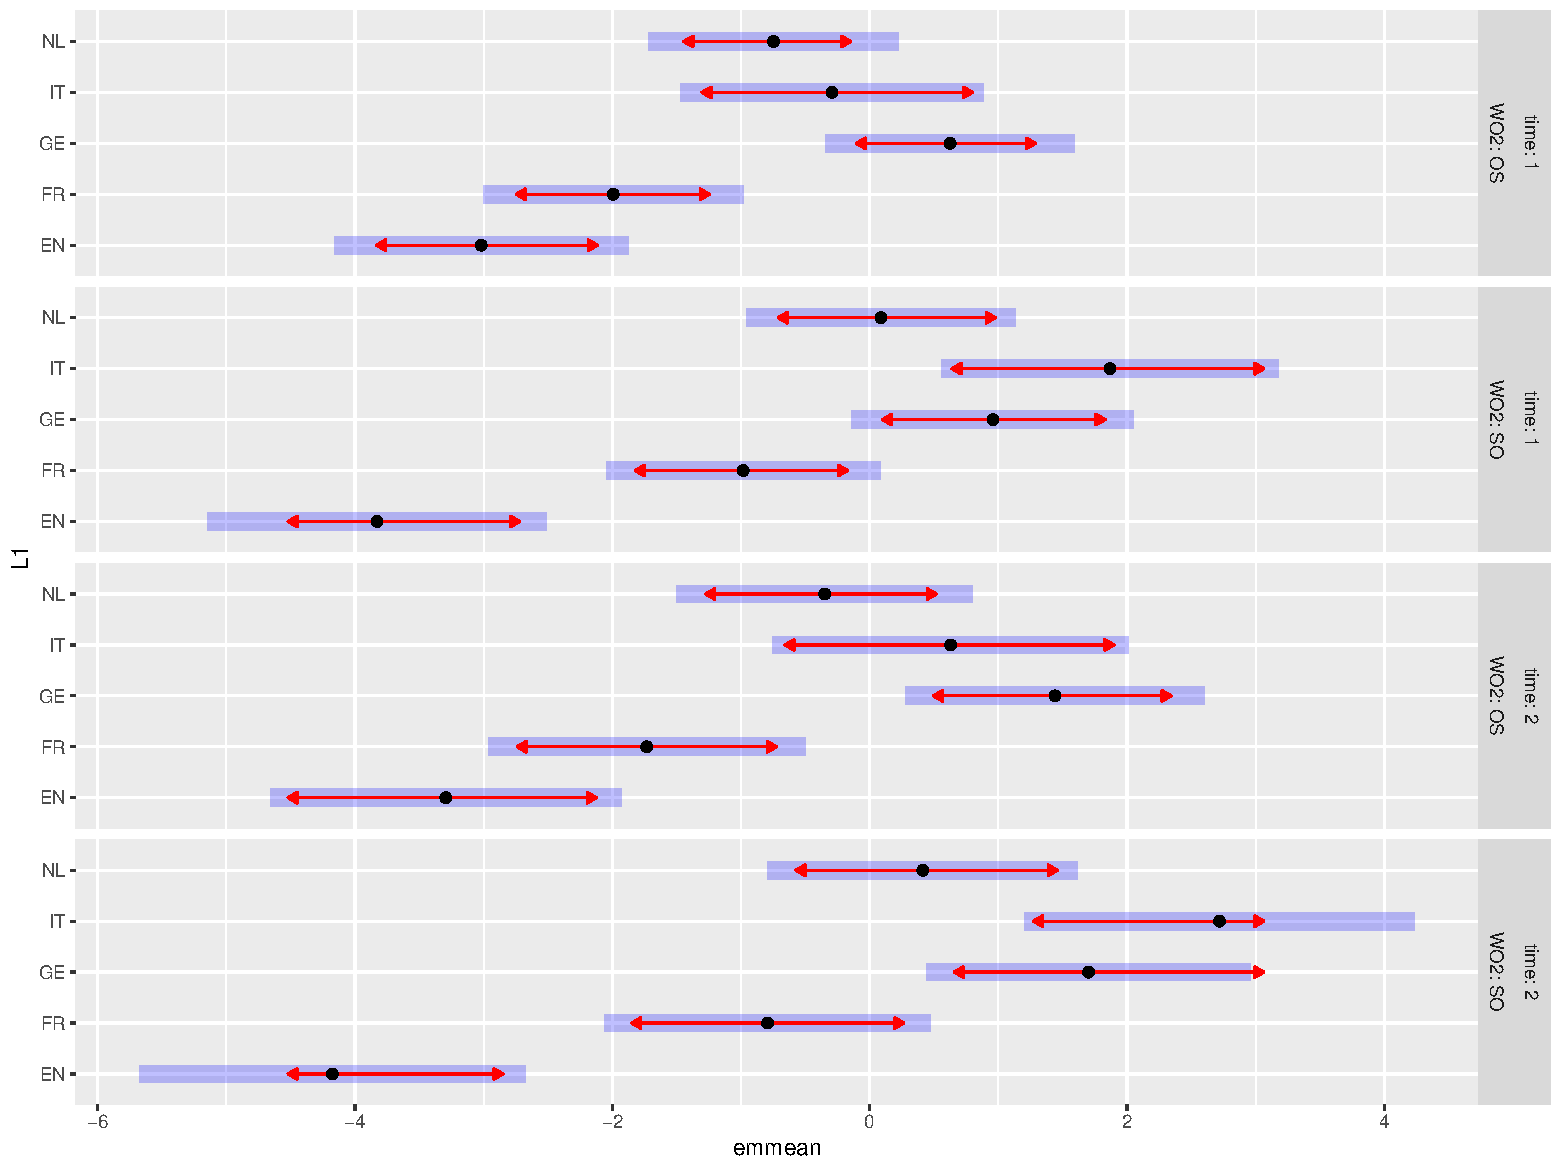
\includegraphics[width=\textwidth]{figures/04-3.pdf}
    \caption{Pairwise comparisons, L1 : word order interaction}
    \label{fig:04:3}
\end{figure}

Turning to the effect of word order (\figref{fig:04:4}), it appears that although SO targets generally produce higher scores (except for the L1 English group), the difference is only significant for the L1 Italian group (p < 0.01 at both test times).

\begin{figure}
    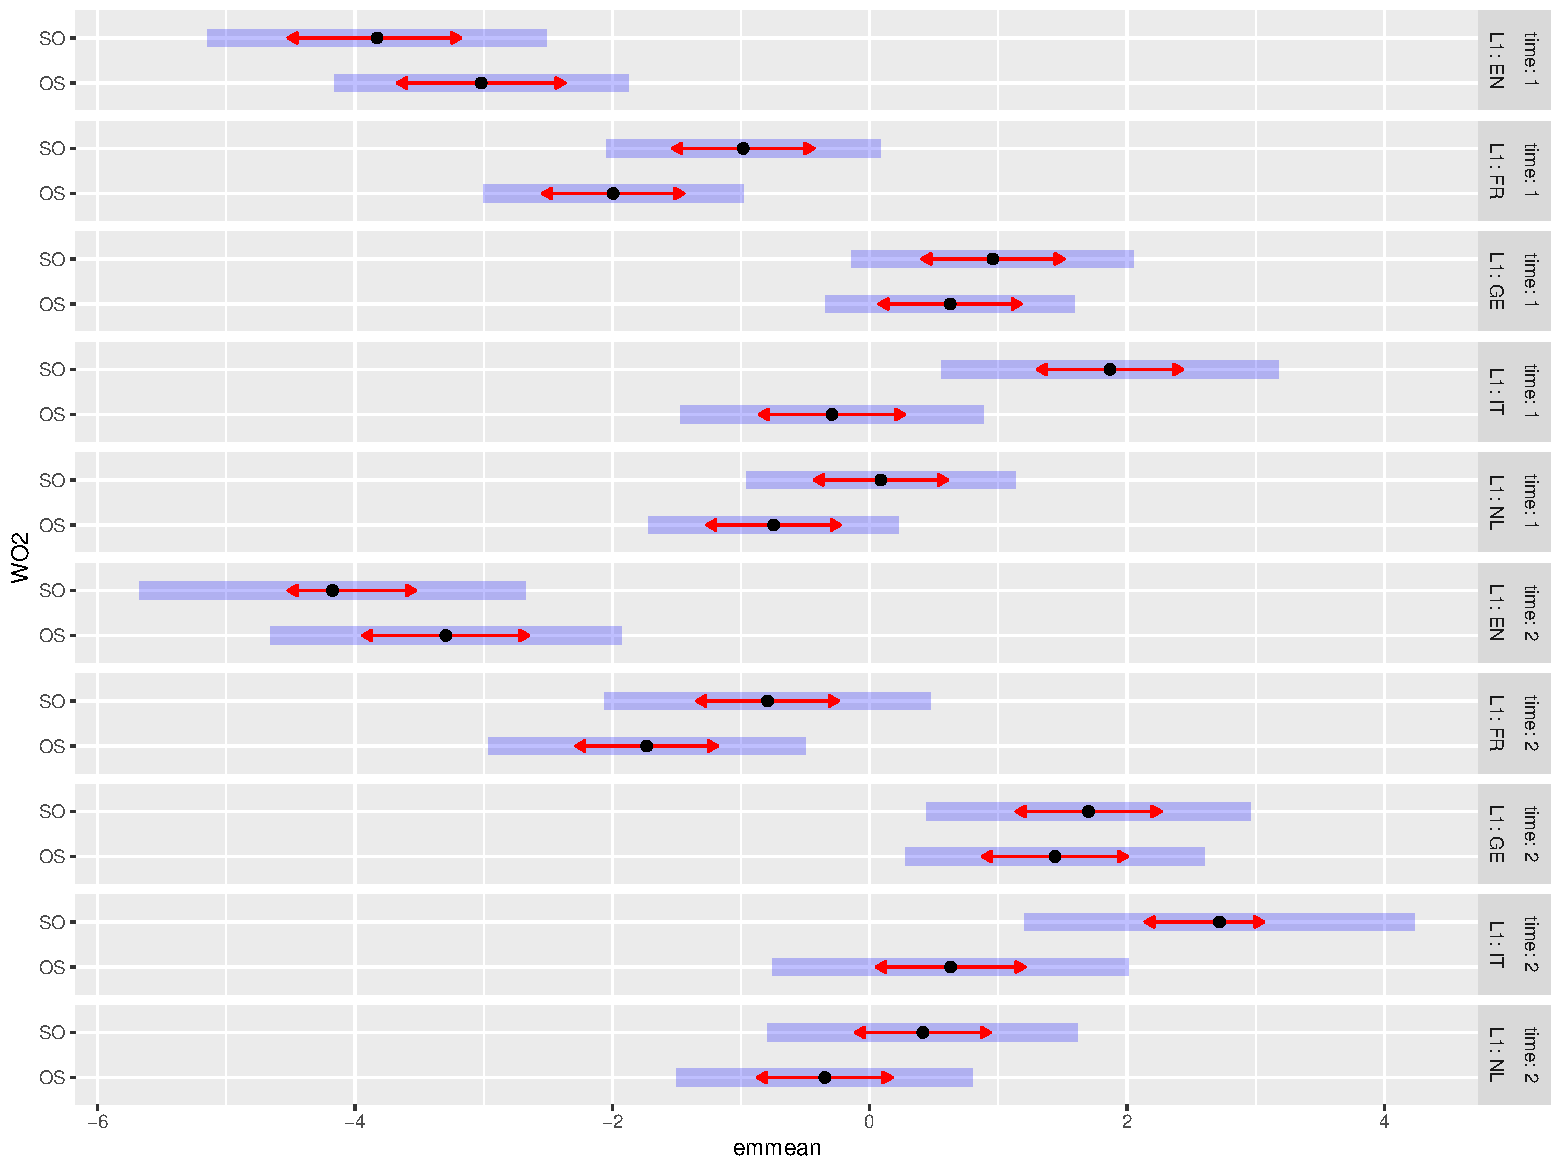
\includegraphics[width=\textwidth]{figures/04-4.pdf}
    \caption{Pairwise comparisons, word order: L1 interaction}
    \label{fig:04:4}
\end{figure}

\subsection{A different perspective}\label{sec:04:2.4}

The analysis presented thus far has shown that certain L1s seem to be associated to higher repetition accuracy when compared to other languages: for instance, French speakers scored on average 0.16 at T1 on the repetition of -[e], whereas the Italians scored 0.55. From this one might conclude that L1 Italian has a positive effect on processing accuracy. These, however, are but mean values, collapsing the results of an entire group. But individual learner performance may vary greatly even within the same L1 group, making the idea of a ``group interlanguage'' quite problematic. Thus, alongside group averages, which may be informative as to the role of a given L1 on the average groups scores, it seems worthwhile to describe learners in terms of their individual processing strategies, operationalised as a set of scenarios. Such outcome would be particularly welcome for an analysis rooted on the Learner Variety theoretical paradigm. Therefore, individual profiling will be used throughout the book to present an alternative view to inferential statistics: it is argued that combined, the two methods may contribute to a better description and interpretation of the data. The present section describes the rationale of this approach.

Within this study, processing profiles may be seen as belonging to three scenarios: 

\begin{itemize}
    \item[a)] learners rely on a single uninflected word-form of each lexical item, with no morphological variation;
    \item[b)] learners may have \textit{noticed} some morphological variation in the input, but they cannot make sense of it based on a systematic rule. Therefore, these learners will supply the basic and inflected word-forms with no apparent regularity;
    \item[c)] learners regularly produce correctly inflected word-forms.
\end{itemize}

Scenario b) might be called chance performance, roughly equivalent to guessing. With only two values to choose from (-[a] and -[e]), accuracy rates should be around 50\%. Scenario a) is \textit{below} chance: learners who behave in this way are not guessing, but applying a systematic principle, which, alas, is not compatible with the target language and thus produces accuracy rates tending to 0\%. Specifically, this principle maintains that all feminine nouns, independently of their syntactic function, are characterised by word-final -[a]. Syntactic functions are expressed by the position of a noun in the utterance.

Finally, scenario c) is \textit{above} chance: learners systematically apply a principle of case marking which is apparently coherent with the regularities of the target language, although in an EI test the possibility cannot be ruled out that target-like performance in fact derives from particularly developed phonological memory.

In order to assign learners to the corresponding scenarios, one needs to statistically compute the probability of observing a given result on the basis of a statistical distribution which appropriately models the task at hand. The binominal distribution describes the probability of obtaining either of two values (conventionally 0 and 1) out of a given number of trials, as in the throwing of a coin. Statistical tests based on this distribution make it possible to answer such questions as ``what is the probability of obtaining head six times if one throws a coin eight times?''. If the probability is too small, conventionally below 5\%, one may conclude that the coin is not fair, i.e. that it is biased towards a particular result. In the present experiment, the same question would sound as follows: ``what is the probability that a learner, without applying a morphosyntactic principle, produced six instances of correct case-marking over eight trials?'' Again, if the probability is too small, one should conclude that performance is not random, i.e. that the learner is applying a morphosyntactic principle.

The modelling of the EI task as a coin throwing experiment may seem questionable on several grounds. Indeed, such an approximation is fairly intuitive in the context of a forced-choice response task, such as the Comprehension task described in Chapter 5, in which learners are simply asked to select the correct alternative out of two possible responses. If they pay no attention at all to the target sentence, and only chose pictures through guessing, then the probability that either picture is selected should be 50\%. This is not the case in the EI task, in which participants are required to actively produce output, the model for which (i.e., the expected response) is provided in the stimulus sentence. 

Moreover, the two possible answers [a] and [e] may not be equally probable or available to the learner. In fact, as it will be shown in \chapref{sec:8}, [a] seems to be the unmarked, basic word-form of lexical items, so that if either ending tends to overextend onto the other, most probably it will be [a] overextending onto [e]. More generally, it is common for initial learner varieties to overextend any given word-form onto all others: clearly, the overextended value should be seen as more probable. In the present context, repeating [e] should require a conscious effort on the side of the learner, thus mirroring an intentional strategy.

Finally, the guessing of a binary value relies on the assumption that the trial may only result in two values. This is indeed the rationale of the VILLA EI test, in which the target structure only opposes [a] to [e]. However, it is impossible to tell whether or not learners were aware that the task only targeted two inflectional endings, especially if one considers that it also included a variety of other structures as distractors: learner output thus may be potentially more varied than that, as even in the limited VILLA input lexical items occur in more than just two word-forms. In sum, the possibility that learners performed the task by guessing alone might seem rather remote.

While this all is true, in principle, the reality is slightly different. The unmarkedness of [a] certainly contributes to explaining why [e] repetition scores tend to zero in some learners, who consistently produced the alternative ending in all contexts. Intermediate scores, however, fit into this picture less well and suggest that target items do imply a choice between [a] and [e], at least in some learners. Regarding the argument that if learners were guessing, then they would produce more than just two endings, it appears that the cases in which learners produce an ending other than -[a] or -[e] (with the exclusion of centralised -/ə/) are extremely rare. After all, the EI task does include a stimulus question in which the expected response is provided. If participants listen carefully to these sentences (which is obviously a prerequisite for the successful completion of the task), they may notice that a) target nouns exhibit some variation across target sentences, and b) that variation only contrasts [a] to [e]. Thus, it does not seem unlikely that the set of possible endings in the learner’s mind only comprises [a] and [e], even though other forms occur in the input. Nevertheless, this does not imply that the learner has already identified the regularity which governs their distribution in the input. If that is the case, then the learner might know that either [a] or [e] is required in the task, but will not be able to tell which should be supplied in the individual target sentences: under these circumstances, randomly supplying either ending, i.e. guessing, may indeed sound like a realistic strategy.

To summarise, one should first ask whether or not the individual learner noticed that target nouns vary in their inflectional ending, the possible options being [a] and [e]. If not, the learner will consistently apply a positional principle, so that the statistical test described above becomes superfluous.

If, in contrast, the learner has noticed that there is some variation, two scenarios are again possible:  a) it may be that the regularity underlying the distribution of the two endings has already been identified, and that morphosyntactic marking in the output is conscious and systematic; or b) if the regularity is still unclear, endings may be supplied randomly or at least unsystematically. The statistical test described above should be used to distinguish learners who at a given test time behave according to scenario a) or b). 

To exemplify, \tabref{tab:04:4} describes each observation in terms of participants, L1, word order and time: for each relevant combination, then, it provides the number of correct responses, the number of trials and the resulting mean accuracy. Finally, the column “EI\_p” indicates the probability of obtaining a value equal to or \textit{greater} than that observed in the data if the learner performed the task by guessing. This last value is computed based on the upper tail of a binomial distribution defined by the number of correct responses (“EI\_correct”), the total number of trials (“EI\_trials”) and a probability value set at 0.5. The lower the value, the less likely it is that the learner could obtain such a score or a greater one by mere guessing: in other words, this is the probability of rejecting the null hypothesis that “the learner’s repetition of [e] was \textit{not} systematic and intentional” when this is in fact true. Clearly, the output of the test makes little sense in the extreme case in which the learner provided no instances of [e]. The opposite extreme case in which the learner only provided correct repetitions of [e] is also hard to interpret, as the test indicates that the probability of obtaining a score greater than that observed (which is not possible, given the limited number of trials in the task) is 0. For all intermediate cases, the test verifies how likely it is that the outcome was not the product of a systematic strategy. In the case of 7 correct responses out of 8, this probability is close to 0; the fewer the correct repetitions, the more likely it is that no systematic strategy was applied.

\begin{table}
    \begin{tabularx}{\textwidth}{Xrrrrrr}
    \lsptoprule
     Subject & WO & Time & EI\_correct & EI\_trials & EI\_mean & EI\_p\\
     \midrule
     2102 & OS & 2 & 0 & 8 & 0.00 & 1.00\\
     2101 & SO & 2 & 1 & 7 & 0.14 & 0.94\\
     2104 & OS & 1 & 2 & 8 & 0.25 & 0.86\\
     2118 & OS & 1 & 3 & 6 & 0.50 & 0.34\\
     3106 & OS & 2 & 6 & 8 & 0.50 & 0.03\\
     5105 & SO & 1 & 7 & 8 & 0.88 & <.00\\
     2108 & SO & 1 & 8 & 8 & 1.00 & 0\\
    \lspbottomrule
    \end{tabularx}
    \caption{Determining above-chance performance}
    \label{tab:04:6}
\end{table}

A word of caution is needed on the possibility of type 1 errors. In the traditional approach, the 0.05 threshold represents the risk which one is willing to accept that what looks like an identifiable tendency in the data (e.g. group A performs better than group B) is in fact due to chance and does not apply to the entire population, but only to the specific sample under examination. Since the present analysis is also based on a statistical test, the same risk is applies here. However, in the present case the 0.05 risk concerns not the entire group (which is not set a priori), but the individual learner: there is a 0.05 possibility that a learner whose performance was classified as "above chance accuracy" in fact did not apply any systematic principle, and only had some lack while performing the task randomly. Theoretically, the reverse risk also exists, whereby learners did attempt to apply a systematic principle, but failed to do so, but in the context of the present experiment, this situation seems hardly explainable. 

In the present analysis, learners are not grouped a priori (as in a treatment vs. non treatment experiment), but based on their performance. Since there is a 0.05 probability that each learner was assigned to the wrong group because of a statistical error, the exact number of learners comprised in each group should be treated with some care.

\subsection{Repetition of -[e]: a comprehensive picture}\label{sec:04:2.4.1} %promoted subsubsection to subsection
The analysis presented so far has failed to provide a comprehensive picture of the behaviour of individual learners across time and word order. This information is provided in \figref{fig:04:5}, where each learner is synchronically described in terms of performance at T1 \textit{and} T2, or on SO \textit{and} OS targets. The graph was created using the statistical software R \citep{RCoreTeam2017} and the packages \textit{wordcloud} \citep{Fellows2014} and \textit{extrafont} \citep{Chang2014} and should be read as follows.

The area is divided into four large squares, representing learner behaviour at T1 in terms of performance on OS (horizontal axis, black) and SO (vertical axis, red) targets. Learners are assigned to the corresponding square depending on whether their performance at T1 differed significantly from chance (upper half of the graph) or not (lower half). 

Each large square is further divided into four smaller ones, which describe learner performance at T2 based on the same rationale. The combination of the square in which the learners lies at T1 (large square) and T2 (small square), in this order, determines the \textit{scenario} in which they fall. Scenario 1:3, for instance, identifies the large square no. 1 and the small square no. 3.

In determining learner processing strategies and their evolution over time, one should proceed as follows. First, identify in which main square the learner is found. If, for example, a learner is in the large square no. 1, that means that the output at T1 differed significantly from chance on both OS and SO targets. Then look at the smaller square in which the learner lies. If, in our example, it is square no. 3, then at T2 the output of that learner was still different from chance on OS targets, but no longer so on SO ones.

\begin{figure}
    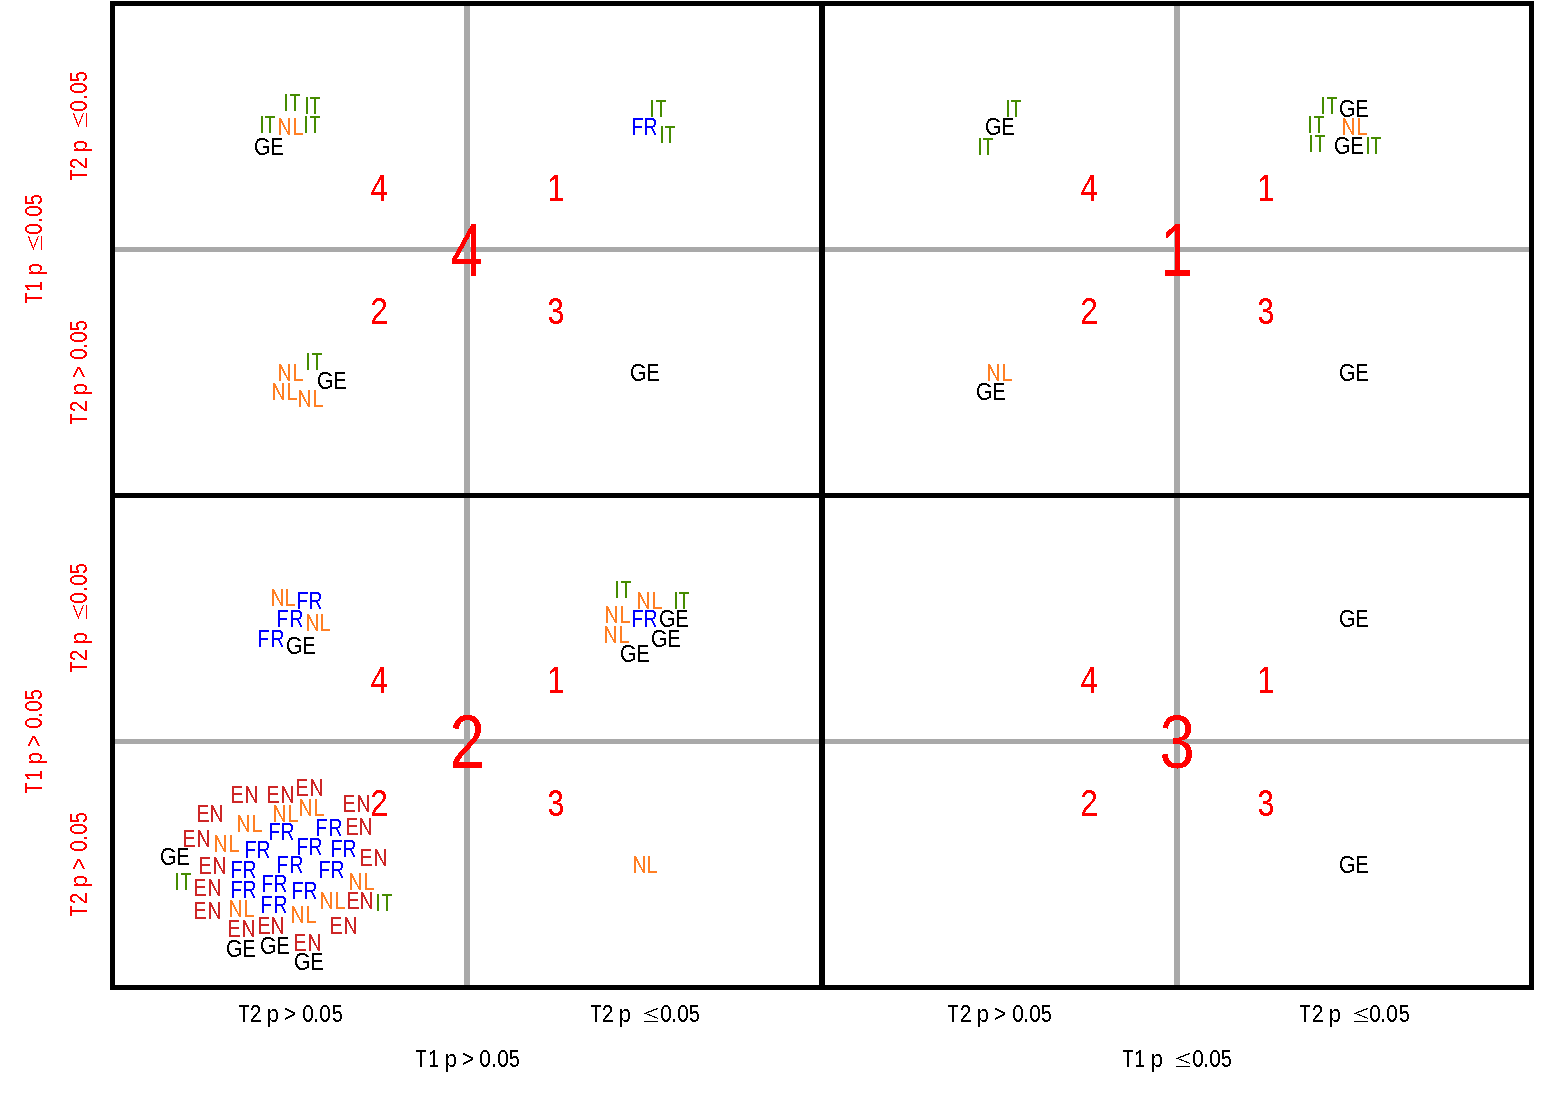
\includegraphics[width=\textwidth]{figures/04-5.pdf}
    \caption{EI task, [e] targets, individual processing strategies}
    \label{fig:04:5}
\end{figure}

The graph can be used to place SO and OS word orders in a hierarchy. At both test times, squares 1 and 2 represent extreme cases: square 1 contains learners who process both types of targets with above chance level accuracy; square 2 those who perform at or below chance level. Among the latter, 9 improved on both types of targets at T2 (scenario 2:1), while 6 showed an improvement on SO targets alone (scenario 2:4). A single participant improved on OS, but not SO targets (scenario 2:3). Scenario 1:1 indicates that all targets were processed with above-chance accuracy at both T1 and T2; scenarios 1:2, 1:3 and 1:4 indicates that performance was above chance at T1, but not so at T2, in which either SO (1:3), OS (1:4) or both types of targets (1:2) did not satisfy the criterion.

Squares 3 and 4 indicate a difference in the processing of word order. It is not unexpected that square 3, in which learners behave above chance on OS, but not SO targets, only comprises 2 learners at T1. The opposite scenario, square 4, comprises 15 learners at T1. 

Overall, it seems that if one value of word order is easier to process, or improves earlier than the other one, then in most cases it is SO. Nevertheless, the vast majority of participants at T1 is found in square 2, indicating chance-level behaviour on both target types.

The graph can also be used to study the evolution of processing strategies in the repetition task over time, depending on the word order of the target sentence. The first obvious observation is that for most learners, there is no evolution whatsoever. The bulk of the data set (42 learners out of 88) can be found in scenario 2:2, which indicates chance behaviour under all conditions (OS and SO targets, at both T1 and T2). This group includes all English L1 learners, most French, about a half of the Dutch, and only a few Italians and Germans. Conversely, 7 learners can be found in scenario 1:1, which indicates the presence of a morpho-syntactic processing strategy all the way from T1 to T2 on both OS and SO targets. Finally, the 6 learners in scenario 4:4 were able to process SO, but not OS targets at T1 and T2 alike.

A few learners show an improvement from T1 to T2. Some change towards more target-like processing strategies: this is the case of scenarios 2:4, 2:3 and 2:1, in which one finds learners who at T1 failed to systematically repeat [e] under any circumstances, but at T2 improved on SO, OS, or both target types, respectively. 

A few participants seem to move away from the target variety: learners in scenario 4:2 processed SO targets above chance at T1, but no longer do so at T2. Other surprising, though rare cases can be found in scenarios 1:3, 1:4 and 1:2: these learners were able to process all targets at T1, but at T2 failed to systematically repeat [e] in SO, OS and all targets, respectively. There might be various explanations for this rare and apparently illogical behaviour. In addition to variables beyond experimental control, such as motivation, tiredness, distractedness, equipment malfunction, such behaviour may be due to border-line scores at T1: even a single additional error thus could have determined their being on either side of the threshold. 

\subsection{Repetition of -[a]}\label{sec:04:2.5}

The data set concerning the repetition of [a] is characterised by an evident ceiling effects for all language groups (\figref{fig:04:6} and \tabref{tab:04:7}).

\begin{figure}
    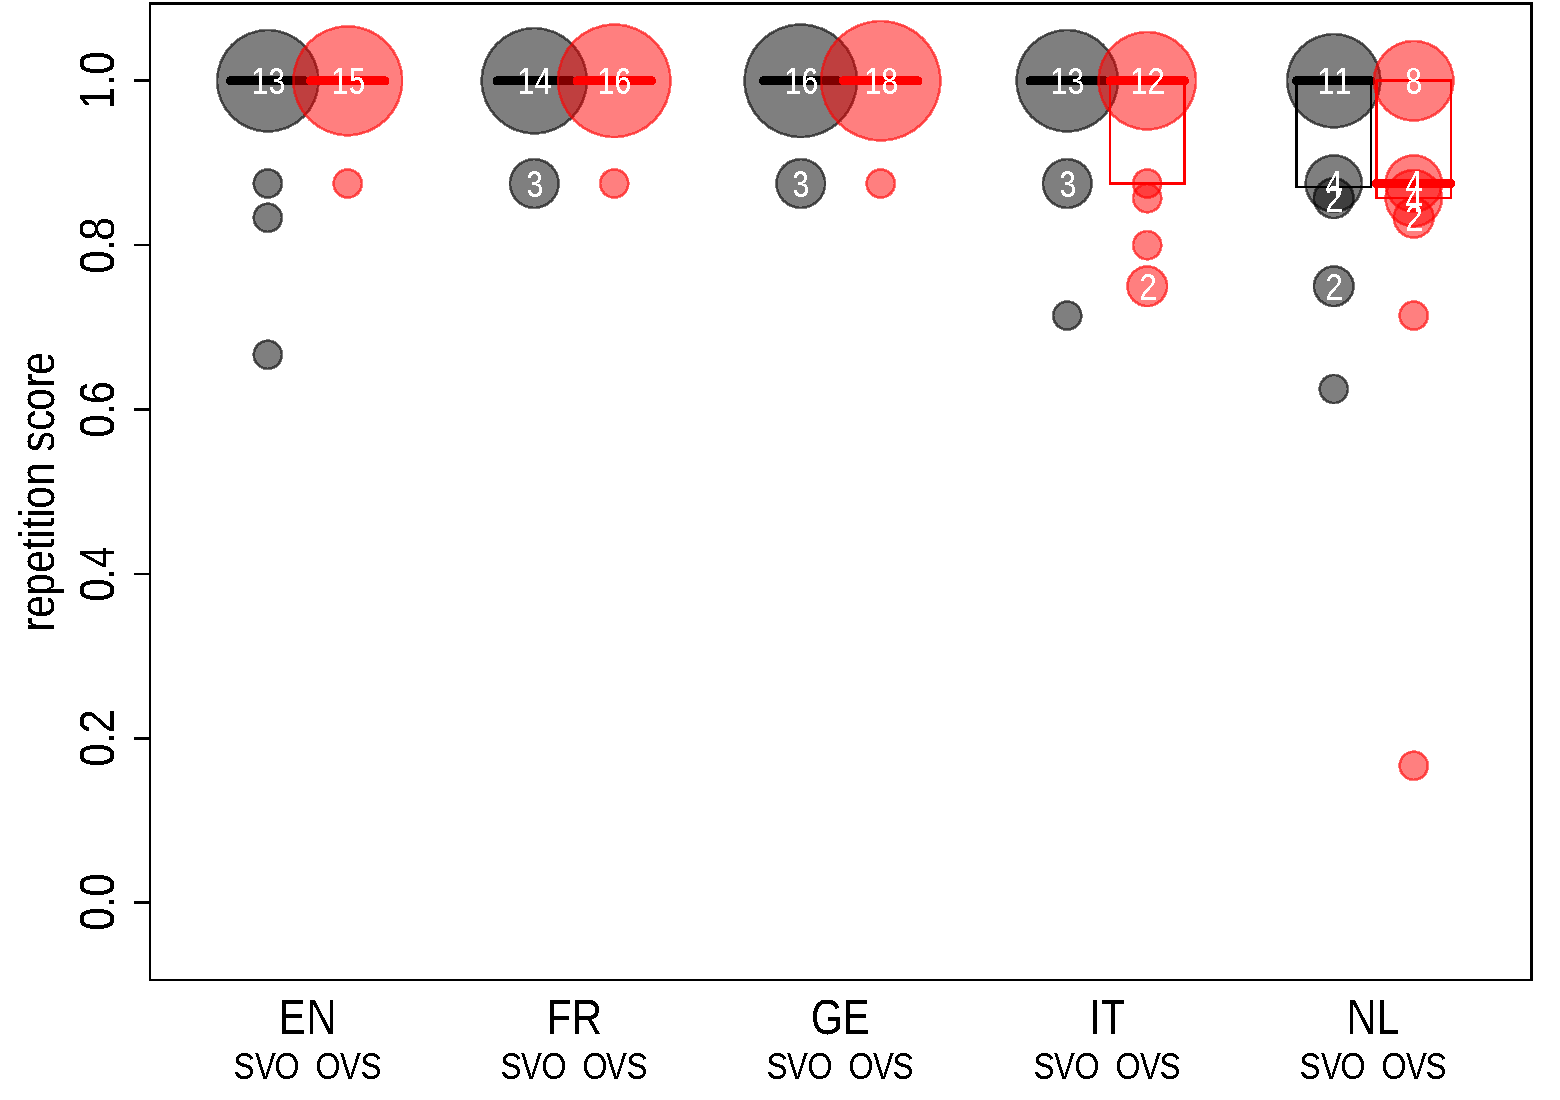
\includegraphics[width=\textwidth]{figures/04-6.pdf}
    \caption{EI task, [a] targets, T1, scores by L1}
    \label{fig:04:6}
\end{figure}

\begin{table}
    \begin{tabularx}{\textwidth}{XXXXXXr}
    \lsptoprule
    & &{SO}& & &{OS}&\\
    L1 & mean & sd & n & mean & sd & n\\
    \midrule
    FR & 0.98 & 0.15 & 127 & 0.99 & 0.09 & 130\\
    GE & 0.98 & 0.14 & 145 & 0.99 & 0.08 & 141\\
    IT & 0.96 & 0.19 & 133 & 0.95 & 0.23 & 128\\
    NL & 0.92 & 0.28 & 154 & 0.88 & 0.32 & 145\\
    EN & 0.96 & 0.20 & 101 & 0.99 & 0.09 & 116\\
    \lspbottomrule
    \end{tabularx}
    \caption{L1 group scores for the repetition of [a], T1}
    \label{tab:04:7}
\end{table}

As detailed in \chapref{sec:3}, in the VILLA input nominative [a] is indeed the most frequent and widespread ending in the paradigm of feminine nouns, in addition to instantiating both the citation form of lexical item as well as the form in which they were first introduced in the input. It is thus hardly surprising that it may overextend onto the much rarer and specialised accusative ending [e]. However, it is interesting to observe that some learners failed to repeat -[a] in all of the cases in which it was required; this tendency also seems to slightly vary across L1s. Since any output different from either [a] or [e] was excluded from the analysis, a failure to repeat [a] necessarily means that the marked ending [e] was produced. It is important to point out that this observation is not equivalent to saying that the accuracy of the repetition of [e] increases: the obligatory occurrences of [a] and [e] constitute different data-sets and are fully independent of each other. An error in the repetition of [a] may result in the two target sentence nouns being marked as [e], or alternatively to the swapping of the expected case endings, if an error is made in the repetition of target [e], too.

Curiously enough, the errors in the repetition of [a] seem to be maintained and even increase in number at T2 (\figref{fig:04:7} and \tabref{tab:04:8}).

\begin{figure}
    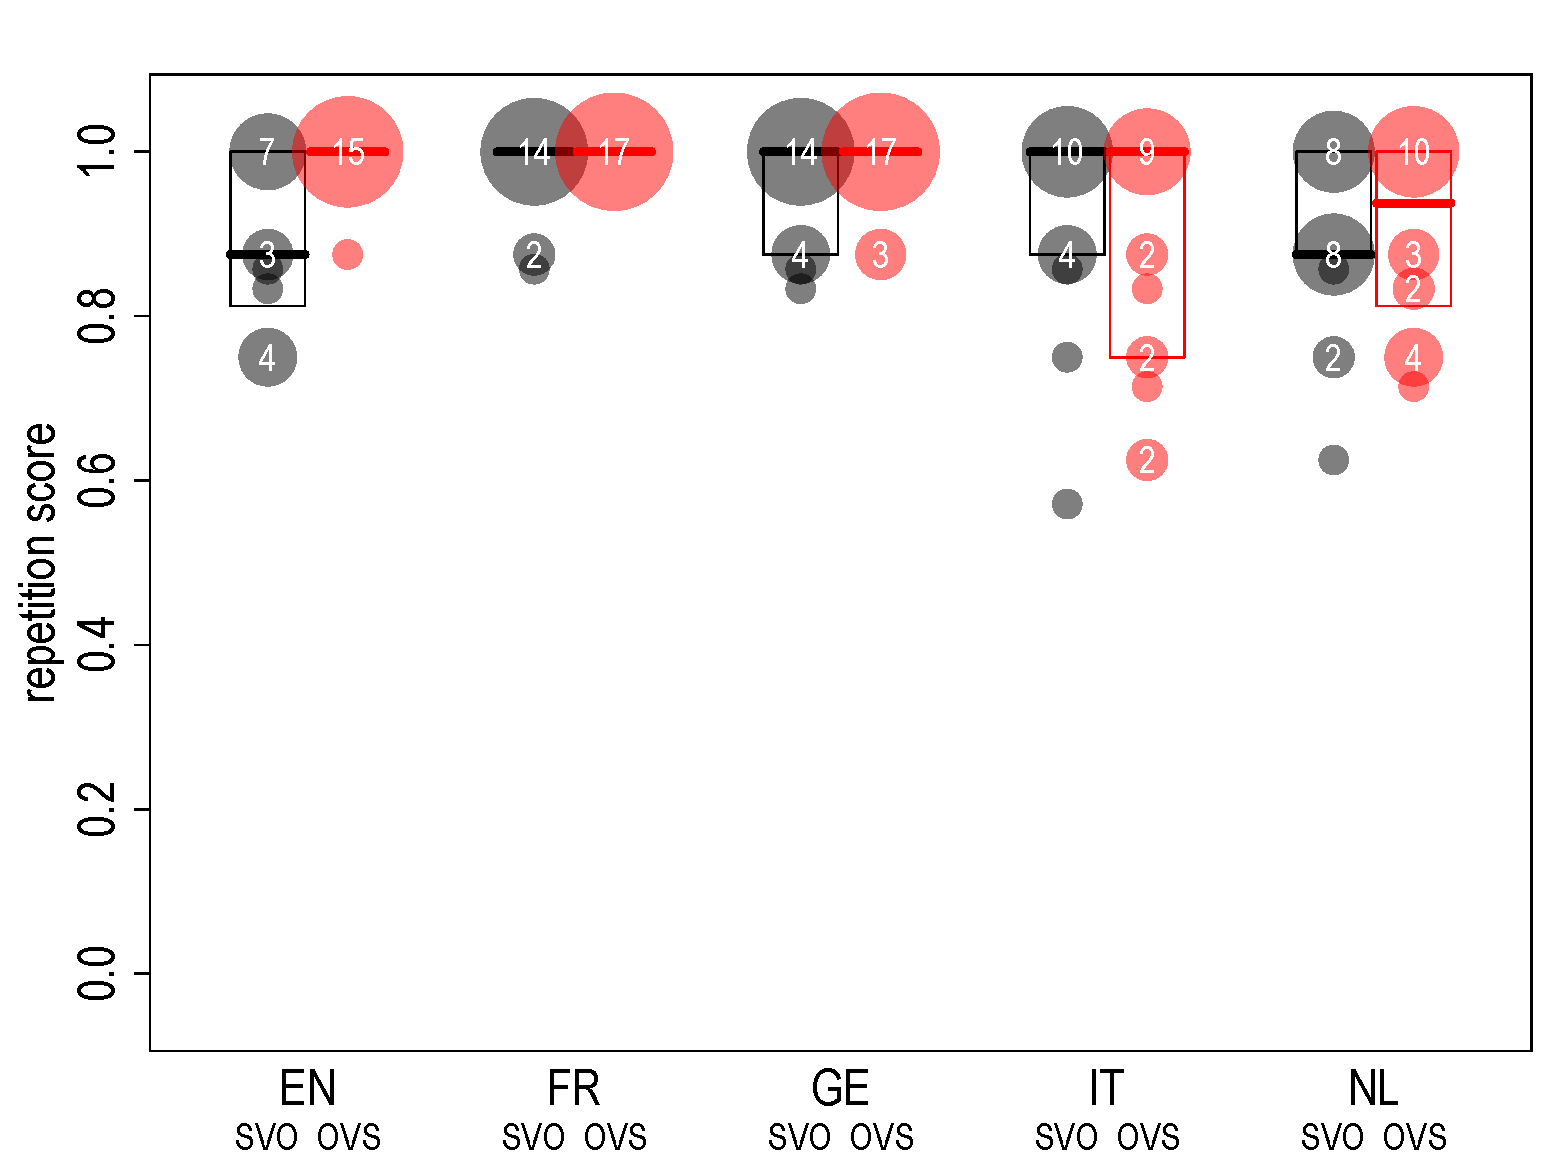
\includegraphics[width=\textwidth]{figures/04-7.pdf}
    \caption{EI task, [a] targets, T2, scores by L1}
    \label{fig:04:7}
\end{figure}

\begin{table}
    \begin{tabularx}{\textwidth}{XXXXXXr}
    \lsptoprule
    &  & {SVO} && & {OVS} &\\
    L1 & Mean & Sd & n & Mean & Sd & n\\
    \midrule
    FR & 0.98 & 0.15 & 132 & 1.00 & 0.00 & 133\\
    GE & 0.96 & 0.19 & 155 & 0.98 & 0.14 & 155\\
    IT & 0.93 & 0.26 & 134 & 0.88 & 0.32 & 128\\
    NL & 0.90 & 0.30 & 158 & 0.90 & 0.30 & 150\\
    EN & 0.89 & 0.31 & 119 & 0.99 & 0.09 & 119\\
    \lspbottomrule
    \end{tabularx}
    \caption{L1 group scores for the repetition of [a], T2}
    \label{tab:04:8}
\end{table}

\tabref{tab:04:9} lists the learners whose probability of correctly repeating -[a] does not differ from chance, again computed for each test time based on a binomial distribution described by the number of correct responses, the number of trials, and a 0.5 chance threshold. These learners do not appear to correctly repeat target [a] with a frequency which could be called systematic; the results are compatible with a strategy of guessing.

The table describes each observation in terms of participants, L1, word order and time: for each relevant combination it provides the number of correct responses, the number of trials and the resulting mean accuracy. Finally, the column “EI\_p” indicates the probability that the learner performed the task by guessing. As discussed in the previous section, this information should be discarded in the extreme cases in which all responses are either correct or incorrect, a scenario whose linguistic interpretation is quite clear anyway. These values are provided for both endings, with the following rationale: if the learner was truly guessing, then one should observe a chance result for both [a] and [e] targets, as these are the only two alternative answers between which one can chose.

\begin{table}
    \fittable{
    \begin{tabular}{l l l ll rr rr rr rr}
    \lsptoprule
    &  &  &  & \multicolumn{2}{c}{EI\_correct} & \multicolumn{3}{c}{EI\_trials} & \multicolumn{2}{c}{ EI\_mean} & \multicolumn{2}{c}{ EI\_p}\\
     Participant & L1 & WO & Time & {}-[a] & \multicolumn{2}{c}{ {}-[e]} & {}-[a] & {}-[e] & {}-[a] & {}-[e] & {}-[a] & {}-[e]\\
     \midrule
     2101 & NL & SO & 2 & 5 & \multicolumn{2}{c}{ 1} & 8 & 7 & 0.63 & 0.14 & 0.14 & 0.94\\
     2102 & NL & OS & 2 & 5 & \multicolumn{2}{c}{ 0} & 7 & 8 & 0.71 & 0.00 & 0.06 & 1.00\\
     2104 & NL & OS & 1 & 1 & \multicolumn{2}{c}{ 2} & 6 & 8 & 0.17 & 0.25 & 0.89 & 0.86\\
     2108 & NL & SO & 1 & 5 & \multicolumn{2}{c}{ 8} & 8 & 8 & 0.63 & 1.00 & 0.14 & 0\\
     2118 & NL & OS & 1 & 5 & \multicolumn{2}{c}{ 3} & 7 & 6 & 0.71 & 0.50 & 0.06 & 0.34\\
     3119 & EN & SO & 1 & 4 & \multicolumn{2}{c}{ 0} & 6 & 7 & 0.67 & 0.00 & 0.11 & 1\\
     5105 & IT & SO & 1 & 5 & \multicolumn{2}{c}{ 7} & 7 & 8 & 0.71 & 0.88 & 0.06 & <.00\\
     5105 & IT & SO & 2 & 4 & \multicolumn{2}{c}{ 7} & 7 & 7 & 0.57 & 1.00 & 0.23 & 0\\
     5106 & IT & OS & 2 & 5 & \multicolumn{2}{c}{ 4} & 7 & 8 & 0.71 & 0.50 & 0.06 & 0.36\\
     5114 & IT & OS & 2 & 5 & \multicolumn{2}{c}{ 3} & 8 & 6 & 0.63 & 0.50 & 0.14 & 0.34\\
     5115 & IT & OS & 2 & 5 & \multicolumn{2}{c}{ 6} & 8 & 8 & 0.63 & 0.75 & 0.14 & 0.04\\
    \lspbottomrule
    \end{tabular}
    }
    \caption{EI task, repetition of –[a] at chance level}
    \label{tab:04:9}
\end{table}

A few comments can be made. First, these learners belong to only three L1 groups, the vast majority being speakers of Dutch or Italian. 5105 appears in the table twice because data were collected at both at T1 and T2. Word order and test time, in contrast, are fairly varied. 

Some learners (2108, 2118, 5105 at T2, 5115) seem to perform better on the repetition of [a]  than of [e]. All other learners conform to the expected pattern, in which repeating [a] appears somewhat easier than repeating [e]. As far as the ending [a] is concerned, the repetition score of some of the participants (2102, 2118, 5105 at T1, 5106) only slightly fails to reach statistical significance: typically, their p value  is 0.06, their mean 0.71, and the correct/total ratio is 5/7, which means that they made two errors out of seven trials. All appear to have missed a trial, which in turn may mean that they supplied an ending other than -[a] or -[e], or alternatively that they failed to repeat an entire target stimulus. In the former case, this behaviour may witness to a certain creativity on their side, which is an indication of system restructuring. The latter case may be speculatively linked to the fact that some participants spent a long time on the distracting phase of the exercise (copying a geometric figure on the answer sheet), which may have somewhat confused their memory of the target. In any case, the 0.05 threshold was set arbitrarily with the purpose of indicating a reasonably small probability, and one could argue that 0.06, although undoubtedly greater, is not so much greater.

These findings may be seen against the bigger picture of -[a] processing. Based on the rationale introduced in the preceding section, \figref{fig:04:8} plots learners according to their performance on the repetition of [a] in OS (horizontal axis, black) and SO (vertical axis, red) targets at T1 and T2.

\begin{figure}
    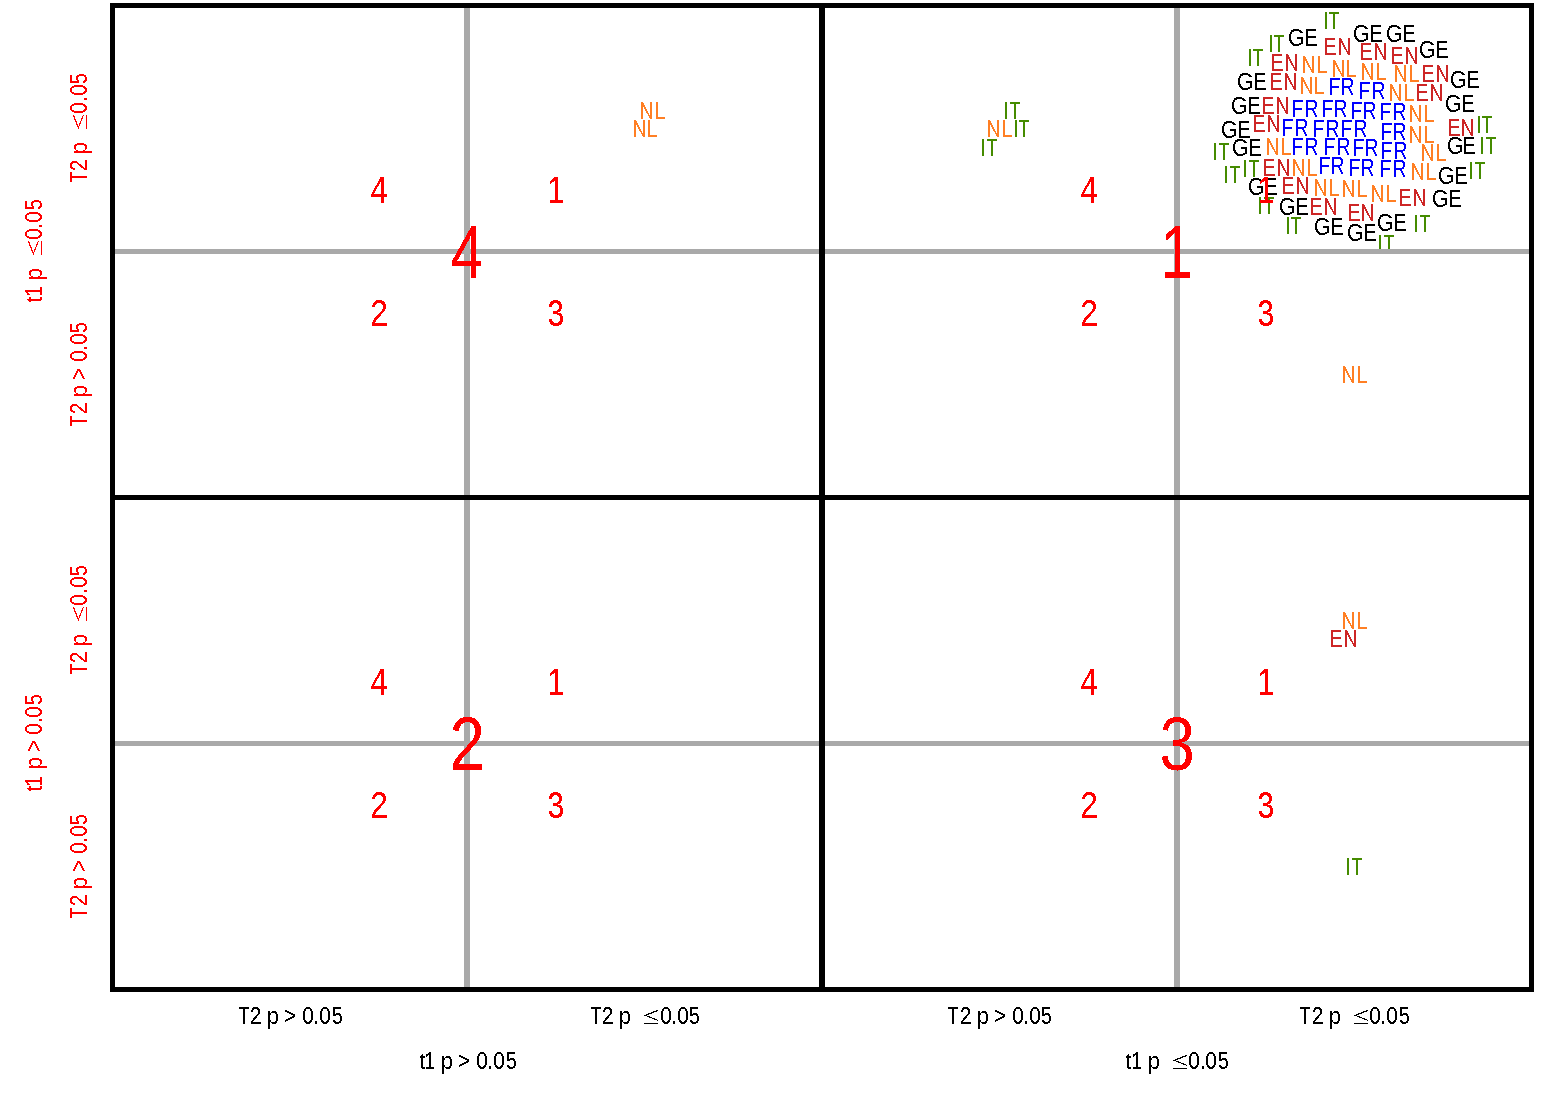
\includegraphics[width=\textwidth]{figures/04-8.pdf}
    \caption{EI task, [a] targets, individual processing strategies}
    \label{fig:04:8}
\end{figure}

Virtually all learners lie in scenario 1:1, which corresponds to scores above chance on OS and SO targets alike at both T1 and T2. The few data-points in other scenarios correspond to the 10 learners just discussed.

\section{Summary}\label{sec:04:3}

The VILLA EI test highlighted several tendencies, which may be summarised as follows:

\begin{itemize}
    \item Morphological marking, i.e. the presence of the non-basic case ending [e] is apparently more widespread in SO than OS targets.
    \item There is a clear effect of cross-linguistic influence in the case of the groups with the highest (L1 German) and lowest (L1 English) scores. The performance of the Italian group is also in line with that of the German participants, although this result was not expected based on contrastive analysis.
    \item Further exposure to the input is clearly beneficial to the development of morpho-syntactic skills.
\end{itemize}

It should be borne in mind that in the absence of a comprehension or a translation task it is impossible to verify what learners really meant to say (if anything) through their output. This in turn raises doubts as to the layer of language effectively targeted by the task: in the absence of this information, it is quite possible that learners did not reproduce the content of the stimulus sentence based on their provisional interlanguage grammar, as assumed by the rationale of the task, but simply repeated it as a string of sounds. Both hypotheses have supporting evidence. The rote repetition hypotheses seems realistic in light of output in which target lexical items are hardly recognisable, which suggests that the learner was not striving to reproduce them based on a mental representation, however approximate, but simply tried to retrieve them as sounds from working memory.

On the other hand, the notable difference between the repetition accuracy of the [e] ending in SO as opposed to OS targets suggest that there may be an effect of syntactic structure, which of course can only be hypothesised if the learner processes targets for meaning and attempts to identify their grammatical structure. Even in this case, however, an alternative perception-based explanation may be proposed: in SO targets, the non-basic [e] ending is found in the maximally salient word-final position, which may facilitate its being noticed and reproduced by learners even in the absence of processing for meaning.

In sum, it seems that while a few clear tendencies may be identified, based on the EI data alone it is impossible to definitively establish whether learners' output is based on morphosyntactic processing or perceptual prominence. In order to better describe the behaviour of the VILLA learners the following two chapters will make use of a comprehension test, whose results will prove useful to interpret the output of the EI task.

\chapter{The comprehension test}\label{sec:4}

\section{Research questions and hypotheses}\label{sec:05:1}

In line with the overall approach of this research, the comprehension test probes the learners' use of case endings by manipulating word order, based on the assumption that while the meaning of SO targets can be derived based on both a positional and a morphosyntactic principle, in the case of OS targets only the morphosyntactic principle is adequate, as the subject of the utterance no longer occurs in its canonical initial position. Two values of OS word order are considered, i.e. OVS and OSV.

The learners’ performance on OS targets thus makes it possible to quantify the extent to which inflectional morphology plays a role in identifying syntactic functions in comprehension.

\section{Results}\label{sec:05:2}
\subsection{Descriptive statistics}\label{sec:05:2.1}

This section first presents descriptive statistics relative to learner data, then attempts to identify any statistically significant tendencies using a statistical model. The following section will interpret the same data from the viewpoint of the approach described in \sectref{sec:04:2.4}, with the aim to detail the individual set of skills of each learner.

\figref{fig:05:1} and \figref{fig:05:2} graphically display learner scores on SVO, OSV and OVS targets at T1 and T2, respectively. The corresponding descriptive statistics are provided in \tabref{tab:05:1} and \tabref{tab:05:2}.

\begin{figure}
    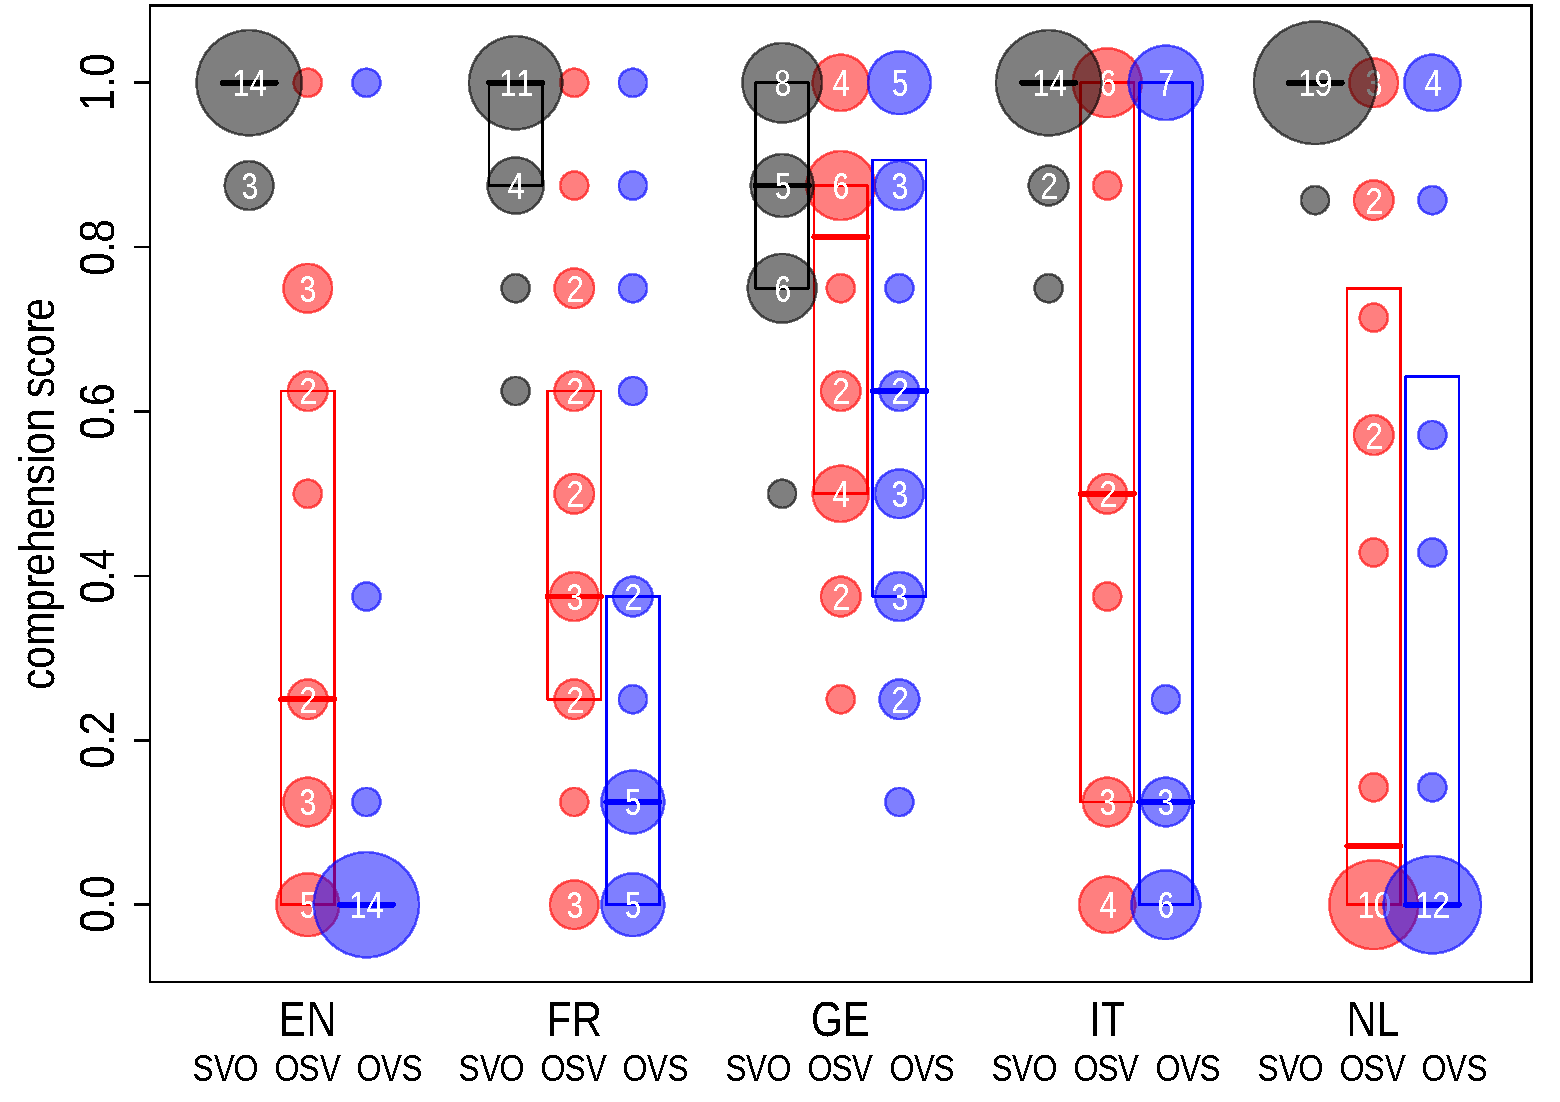
\includegraphics[width=\textwidth]{figures/05-1.pdf}
    \caption{Comprehension test, scores by L1 and word order, T1}
    \label{fig:05:1}
\end{figure}

\begin{table}
    \begin{tabularx}{\textwidth}{XYYYYYYY}
    \lsptoprule
    L1 &  & \multicolumn{2}{c}{SVO} & \multicolumn{2}{c}{OSV} & \multicolumn{2}{c}{OVS}\\
    & n. & mean & sd & mean & sd & mean & sd\\
    \cmidrule(lr){3-4}\cmidrule(lr){5-6}\cmidrule(lr){7-8}
    EN & 17 & 0.98 & 0.15 & 0.35 & 0.48 & 0.09 & 0.28\\
    FR & 17 & 0.93 & 0.25 & 0.43 & 0.50 & 0.29 & 0.45\\
    GE & 20 & 0.87 & 0.34 & 0.71 & 0.45 & 0.64 & 0.48\\
    IT & 17 & 0.97 & 0.17 & 0.51 & 0.50 & 0.45 & 0.50\\
    NL & 20 & 0.99 & 0.08 & 0.36 & 0.48 & 0.30 & 0.46\\
    mean & {}- & 0.95 & 0.20 & 0.47 & 0.48 & 0.35 & 0.43\\
    \lspbottomrule
    \end{tabularx}
    \caption{Comprehension task, descriptive statistics, T1}
    \label{tab:05:1}
\end{table}

\begin{figure}
    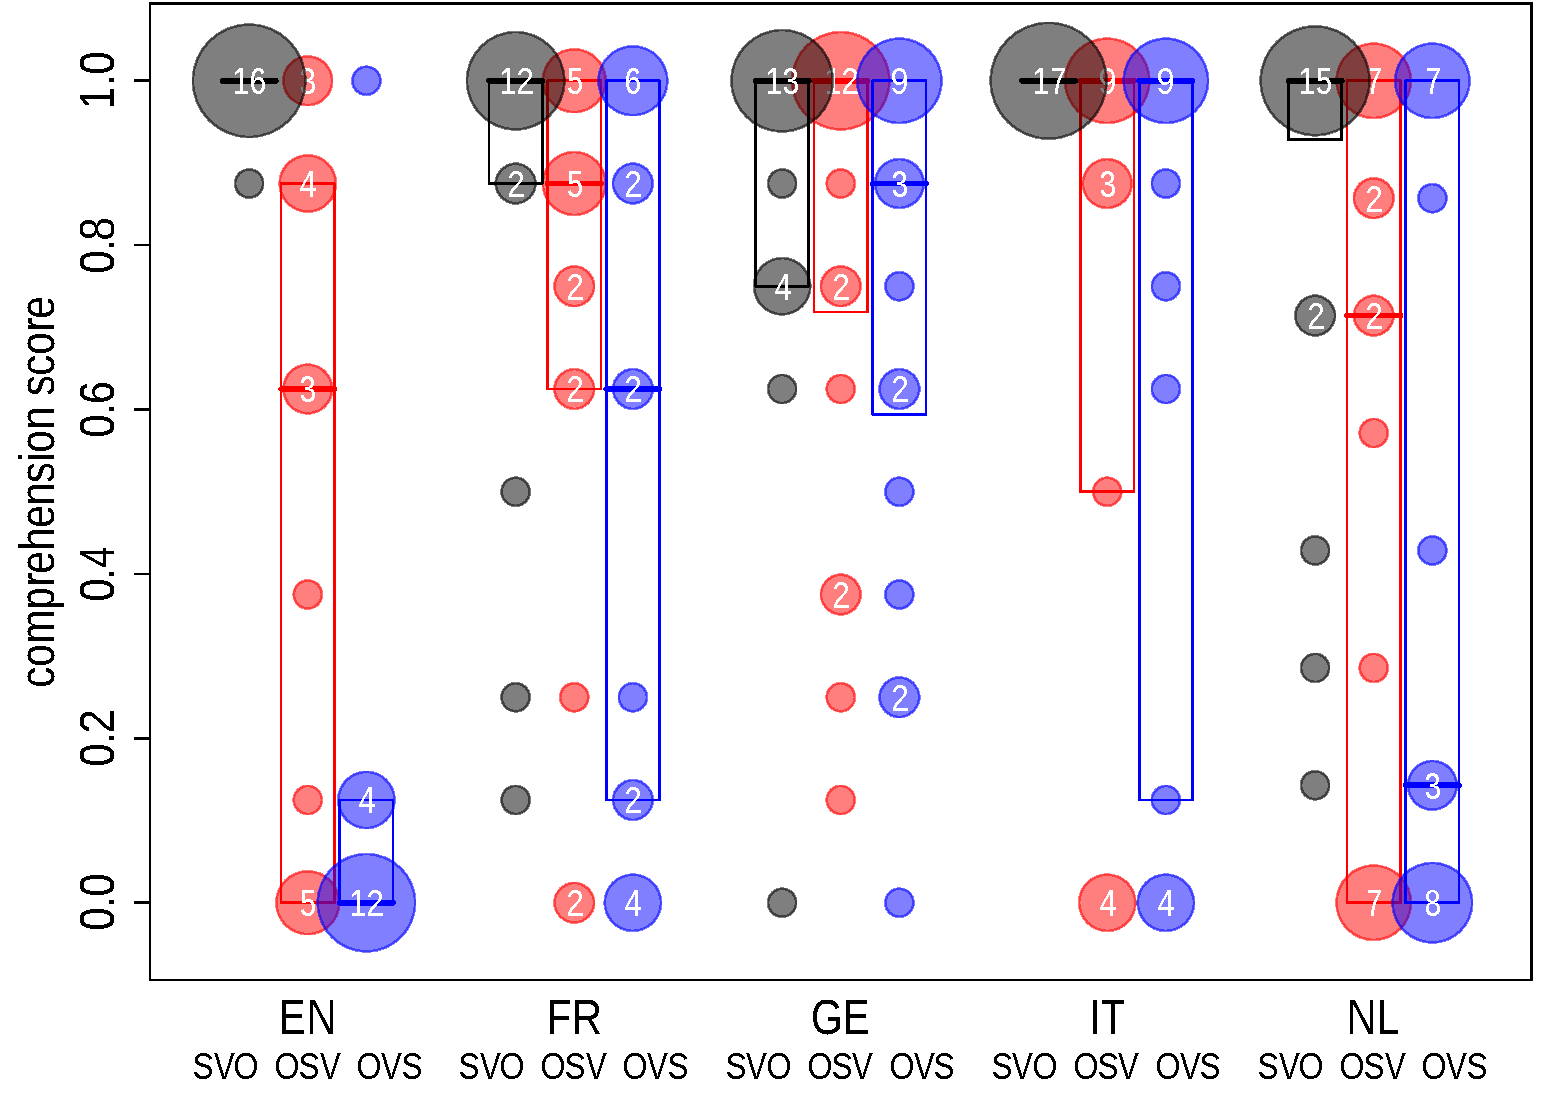
\includegraphics[width=\textwidth]{figures/05-2.pdf}
    \caption{Comprehension test, scores by L1 and word order, T1}
    \label{fig:05:2}
\end{figure}

\begin{table}
    \begin{tabularx}{\textwidth}{XYYYYYYY}
    \lsptoprule
    L1 &  & \multicolumn{2}{c}{SVO} & \multicolumn{2}{c}{OSV} & \multicolumn{2}{c}{OVS}\\
    & n. & mean & sd & mean & sd & mean & sd\\
    \cmidrule(lr){3-4}\cmidrule(lr){5-6}\cmidrule(lr){7-8}
    EN & 17 & 0.99 & 0.08 & 0.52 & 0.50 & 0.08 & 0.28\\
    FR & 17 & 0.86 & 0.34 & 0.72 & 0.44 & 0.55 & 0.49\\
    GE & 20 & 0.87 & 0.33 & 0.80 & 0.39 & 0.75 & 0.43\\
    IT & 17 & 1.00 & 0.00 & 0.71 & 0.45 & 0.66 & 0.47\\
    NL & 20 & 0.86 & 0.34 & 0.55 & 0.49 & 0.43 & 0.49\\
    mean & {}- & 0.92 & 0.22 & 0.66 & 0.45 & 0.49 & 0.43\\
    \lspbottomrule
    \end{tabularx}
    \caption{Comprehension task, descriptive statistics, T2}
    \label{tab:05:2}
\end{table}
\clearpage

A few preliminary remarks can be made based on these descriptive statistics. First, as expected, SO scores are much higher than their OS equivalents in all cases. Curiously, though, the mean scores below 100\% as well as the rather high standard deviations point to the fact that some learners actually made several errors on SVO targets too, which runs contrary to the initial hypotheses. 

Regularities are also observed in the difference between the two OS constituent orders. Accuracy on OSV targets is higher in all cases, the only exception being the German group at T2. The English group stands out in this respect, too, in that the difference between the two values of word order is particularly extreme, and the standard deviation on OVS targets is much lower than in the other L1 groups. Combined, these two pieces of information indicate that compared to OSV targets, English learners perform much worse on OVS ones than the other L1 groups do, and that all learners in this group do so in a rather uniform manner. 

\subsection{Inferential statistics}\label{sec:05:2.2}

A generalised linear mixed model with binomial error structure and logit link function (Likelihood Type 3-test) was fitted to the data using the R package \textit{lme4} \citep{BatesEtAl2015}: fixed effects comprise the L1 (factor, five levels: EN, FR, GE, IT, NL, reference level=EN), word order (factor, binary, reference level=OS) and time (factor, binary, reference level=1) as linear predictors, as well as their two-way interactions: L1:word order, L1:time, and time:word order. 

The rationale for including the interactions is as follows. The learners' ability to identify the syntactic structure of the target is hypothesised to be influenced by target sentence word order, SO generally having a positive effect, OS having a negative effect. In turn, the impact of word order may be modulated by the learner’s L1. Further exposure is thought to be generally beneficial, but the extent to which results improve between T1 and T2 may be also determined by the learners’ L1 (speakers of certain languages improving more markedly than speakers of other languages) and word order (within the same L1 group, either word order may show greater improvement over time). 

To simulate individual variability, finally, the model includes random intercepts for participants and test items as well as interacting random slopes for word order and time. The model output is presented in \tabref{tab:05:3}.

\begin{table}
    \begin{tabularx}{\textwidth}{Xrrr}
    \lsptoprule
    \textit{predictors} & \textit{odds} \textit{ratios} & \textit{CI} & \textit{p}\\
    \midrule
    (intercept) & 0.08 & 0.02~—~0.39 & \textbf{0.002}\\
    time [2] & 3.26 & 0.87~—~12.21 & 0.080\\
    L1 [FR] & 4.97 & 0.63~—~38.99 & 0.127\\
    L1 [GE] & 53.17 & 7.05~—~400.88 & \textbf{<0.001}\\
    L1 [IT] & 11.26 & 1.33~—~95.56 & \textbf{0.026}\\
    L1 [NL] & 3.00 & 0.39~—~23.02 & 0.290\\
    WO2 [SO] & 2367.21 & 332.20~—~16868.10 & \textbf{<0.001}\\
    time [2] * L1 [FR] & 2.86 & 0.45~—~18.22 & 0.265\\
    time [2] * L1 [GE] & 1.87 & 0.30~—~11.64 & 0.504\\
    time [2] * L1 [IT] & 4.30 & 0.57~—~32.21 & 0.156\\
    time [2] * L1 [NL] & 1.51 & 0.24~—~9.62 & 0.665\\
    time [2] * WO2 [SO] & 0.36 & 0.18~—~0.75 & \textbf{0.006}\\
    L1 [FR] * WO2 [SO] & 0.02 & 0.00~—~0.18 & \textbf{0.001}\\
    L1 [GE] * WO2 [SO] & 0.00 & 0.00~—~0.01 & \textbf{<0.001}\\
    L1 [IT] * WO2 [SO] & 0.06 & 0.00~—~0.70 & \textbf{0.025}\\
    L1 [NL] * WO2 [SO] & 0.09 & 0.01~—~0.86 & \textbf{0.036}\\
    \multicolumn{4}{c}{\textbf{random} \textbf{effects}}\\
    σ\textsuperscript{2} & \multicolumn{3}{r}{3.29}\\
    τ\textsubscript{00}~\textsubscript{participant} & \multicolumn{3}{r}{8.33}\\
    τ\textsubscript{00}~\textsubscript{target\_no} & \multicolumn{3}{r}{0.56}\\
    τ\textsubscript{11}~\textsubscript{participant.time2} & \multicolumn{3}{r}{5.63}\\
    τ\textsubscript{11}~\textsubscript{participant.WO2SO} & \multicolumn{3}{r}{6.98}\\
    ρ\textsubscript{01}~\textsubscript{participant.time2} & \multicolumn{3}{r}{{}-0.11}\\
    ρ\textsubscript{01}~\textsubscript{participant.WO2SO} & \multicolumn{3}{r}{{}-0.93}\\
    ICC & \multicolumn{3}{r}{0.73}\\
    N~\textsubscript{participant} & \multicolumn{3}{r}{91}\\
    N~\textsubscript{target\_no} & \multicolumn{3}{r}{24}\\
    \midrule
    observations & \multicolumn{3}{c}{4248}\\
    marginal R\textsuperscript{2}~/ conditional R\textsuperscript{2} & \multicolumn{3}{c}{0.334 / 0.818}\\
    \lspbottomrule
    \end{tabularx}
    \caption{Output model}
    \label{tab:05:3}
\end{table}

The three hypothesised interactions were probed by comparing this full model to three null models, each lacking the single interaction of interest. Statistical significance was assessed based on likelihood ratio tests (\tabref{tab:05:4}). Multiple comparison was addressed using the Holm correction.

\begin{table}
    \begin{tabularx}{\textwidth}{Xrrr}
    \lsptoprule
    predictor & Chisq & Df & Pr(>Chisq)\\
    \midrule
    time : L1 & 2.484 & 4 & >0.05\\
    time : word order & 7.599 & 1 & 0.01\\
    L1 : word order & 35.840 & 4 & <0.01\\
    \lspbottomrule
    \end{tabularx}
    \caption{Comprehension results, single term deletion}
    \label{tab:05:4}
\end{table}

The interaction between time and L1 does not reach statistical significance, but both terms engage in other statistically significant interactions. The latter were explored through pairwise comparisons. In \figref{fig:05:3} and \ref{fig:05:4}, blue bars depict confidence intervals: for any pairwise comparison, two terms differ significantly if the red arrows do not overlap.

\figref{fig:05:3} depicts the interaction between time and word order. No statistically significant difference between T1 and T2 can be observed for SO targets, which indicates no significant improvement in time. The reverse is true for OS targets, in which a statistically significant improvement can be observed between T1 and T2 for all L1 groups except the L1 English group, whose performance does improve in time, but not to a significant extent.

\begin{figure}[p]
    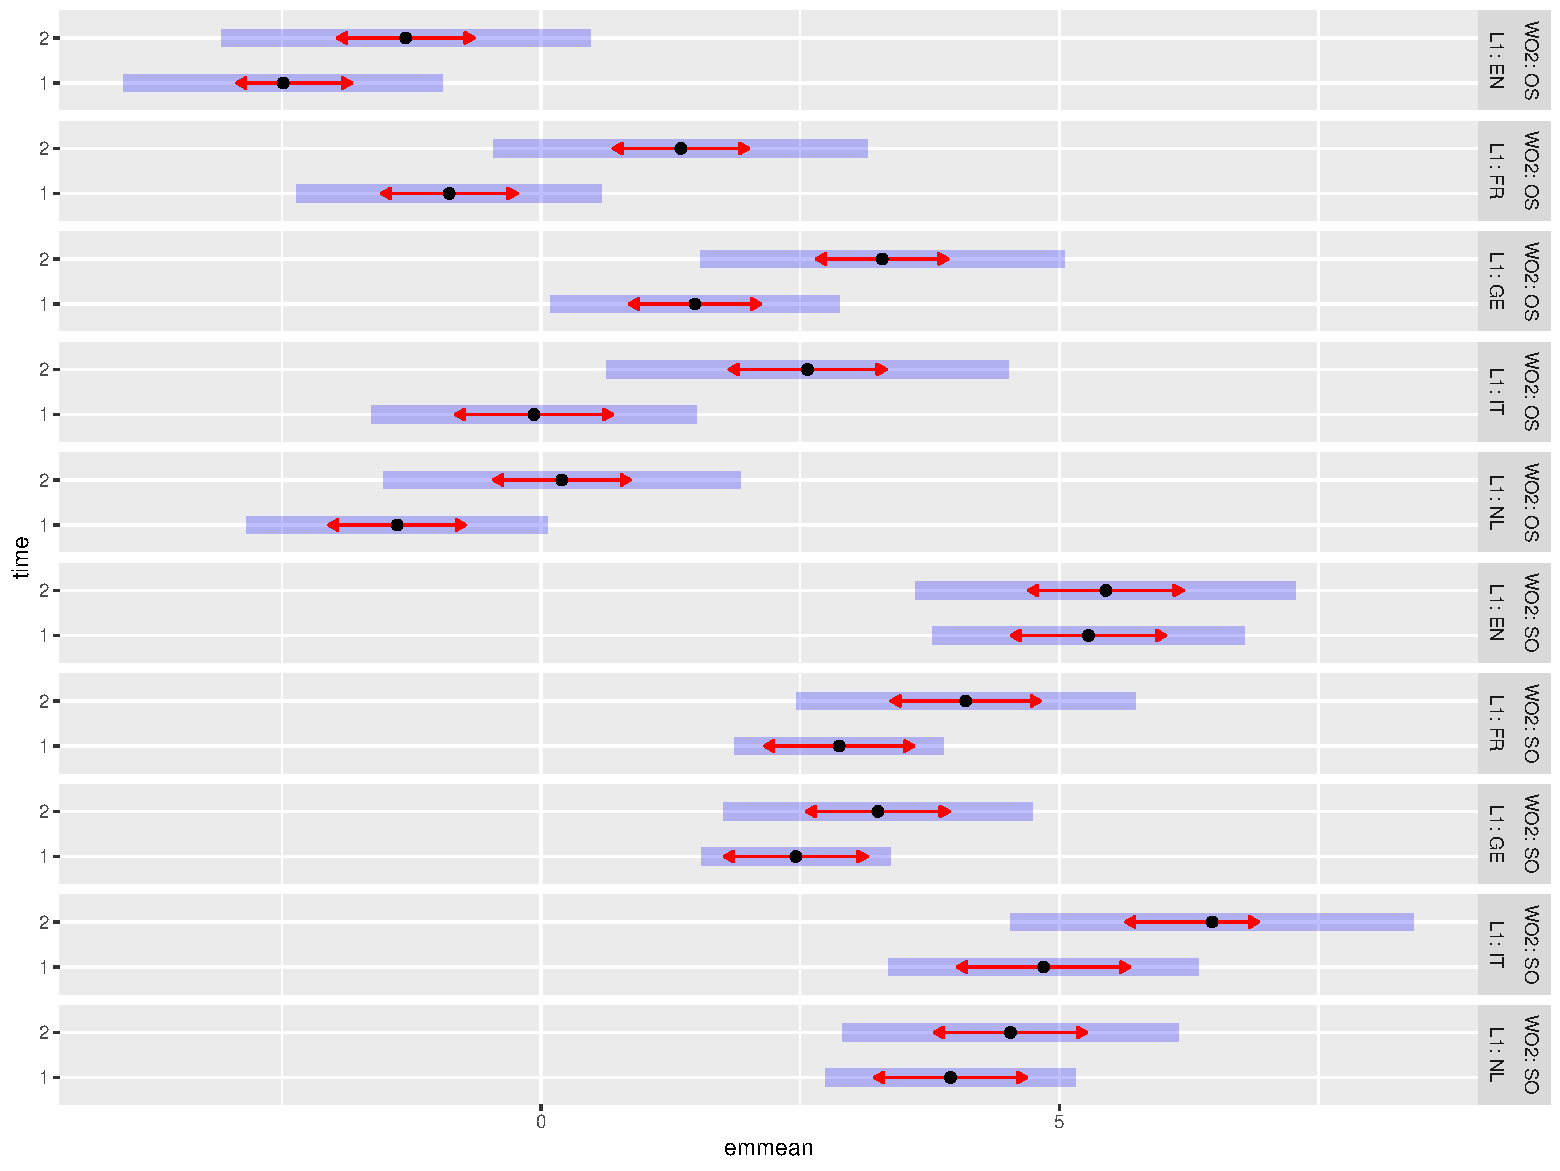
\includegraphics[height=.4\textheight]{figures/05-3.pdf}
    \caption{Pairwise comparisons, effect of time across L1 and word order}
    \label{fig:05:3}
\end{figure}

\figref{fig:05:4} depicts the interaction between L1 and word order. Notable facts are reported in \tabref{tab:05:5}. The symbols “>” and “<” indicate significantly better and significantly worse performance, respectively. Only significant contrasts are reported.

\begin{table}
    \begin{tabularx}{\textwidth}{XX}
    \lsptoprule
    condition & significant contrasts\\
    \midrule
    T1, OS & GE $>$ NL $(p = 0.03)$, EN $(p < 0.01)$\\
    \tablevspace
    T1, SO & GE $<$ IT $(p = 0.01)$, EN $(p < 0.01)$;\newline
            FR $<$ EN $(p = 0.02)$\\
    \tablevspace
    T2, OS & EN < GE $(p < 0.01)$, IT $(p = 0.02)$\\
    \tablevspace
    T2, SO & GE < IT $(p = 0.03)$\\
    \lspbottomrule
    \end{tabularx}
    \caption{Pairwise comparisons, L1: word order (WO) interaction, significant contrasts}
    \label{tab:05:5}
\end{table}

\begin{figure}[p]
    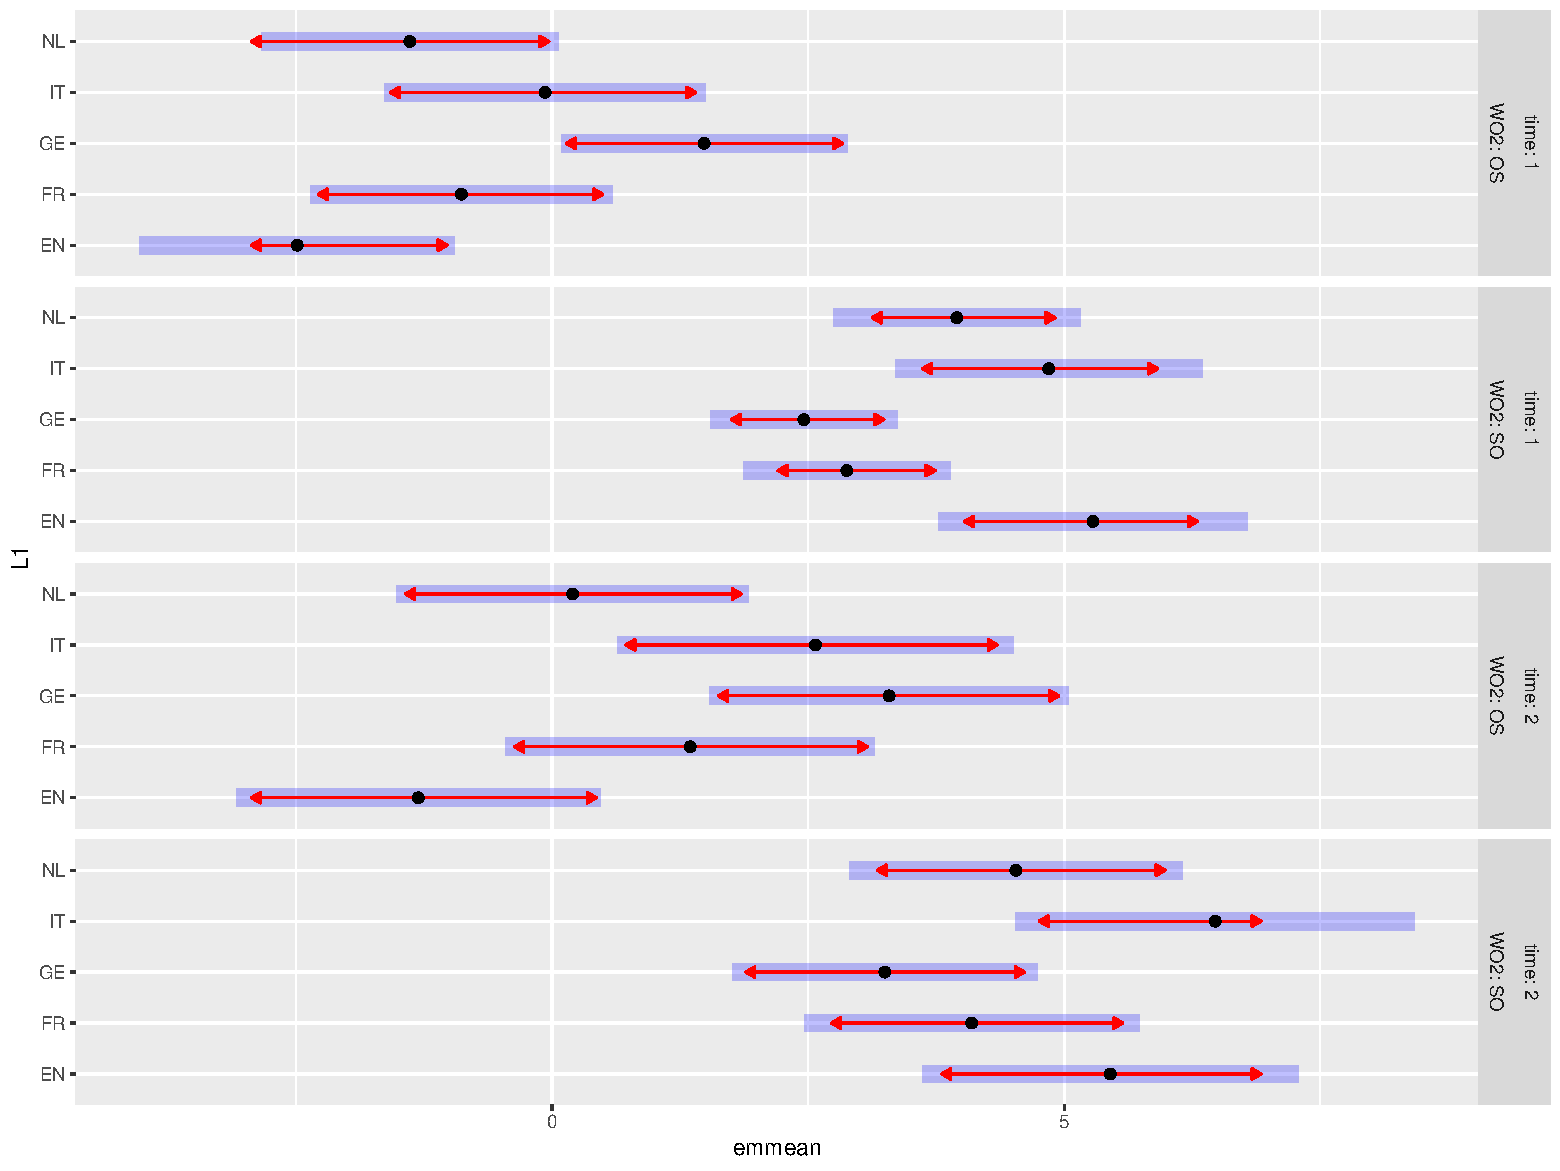
\includegraphics[height=.4\textheight]{figures/05-4.pdf}
    \caption{Pairwise comparisons, effect of L1 across time and word order}
    \label{fig:05:4}
\end{figure}
\clearpage

\subsection{Individual processing strategies}\label{sec:05:2.3}

Based on the approach discussed in \sectref{sec:04:2.4}, this section attempts to compute the likelihood that learners might have performed the Comprehension test with above-chance accuracy, that is, that they responded correctly in such a consistent and systematic way that the existence of a morphosyntactic principle of utterance organisation may be hypothesised.

\figref{fig:05:5} shows the number of participants who can be said to have applied a target-like morphosyntactic principle in their responses to the comprehension task at T1 (target-like behaviour was defined as systematic, above-chance performance). The digits indicate the actual number of participants for each category.

\begin{figure}
    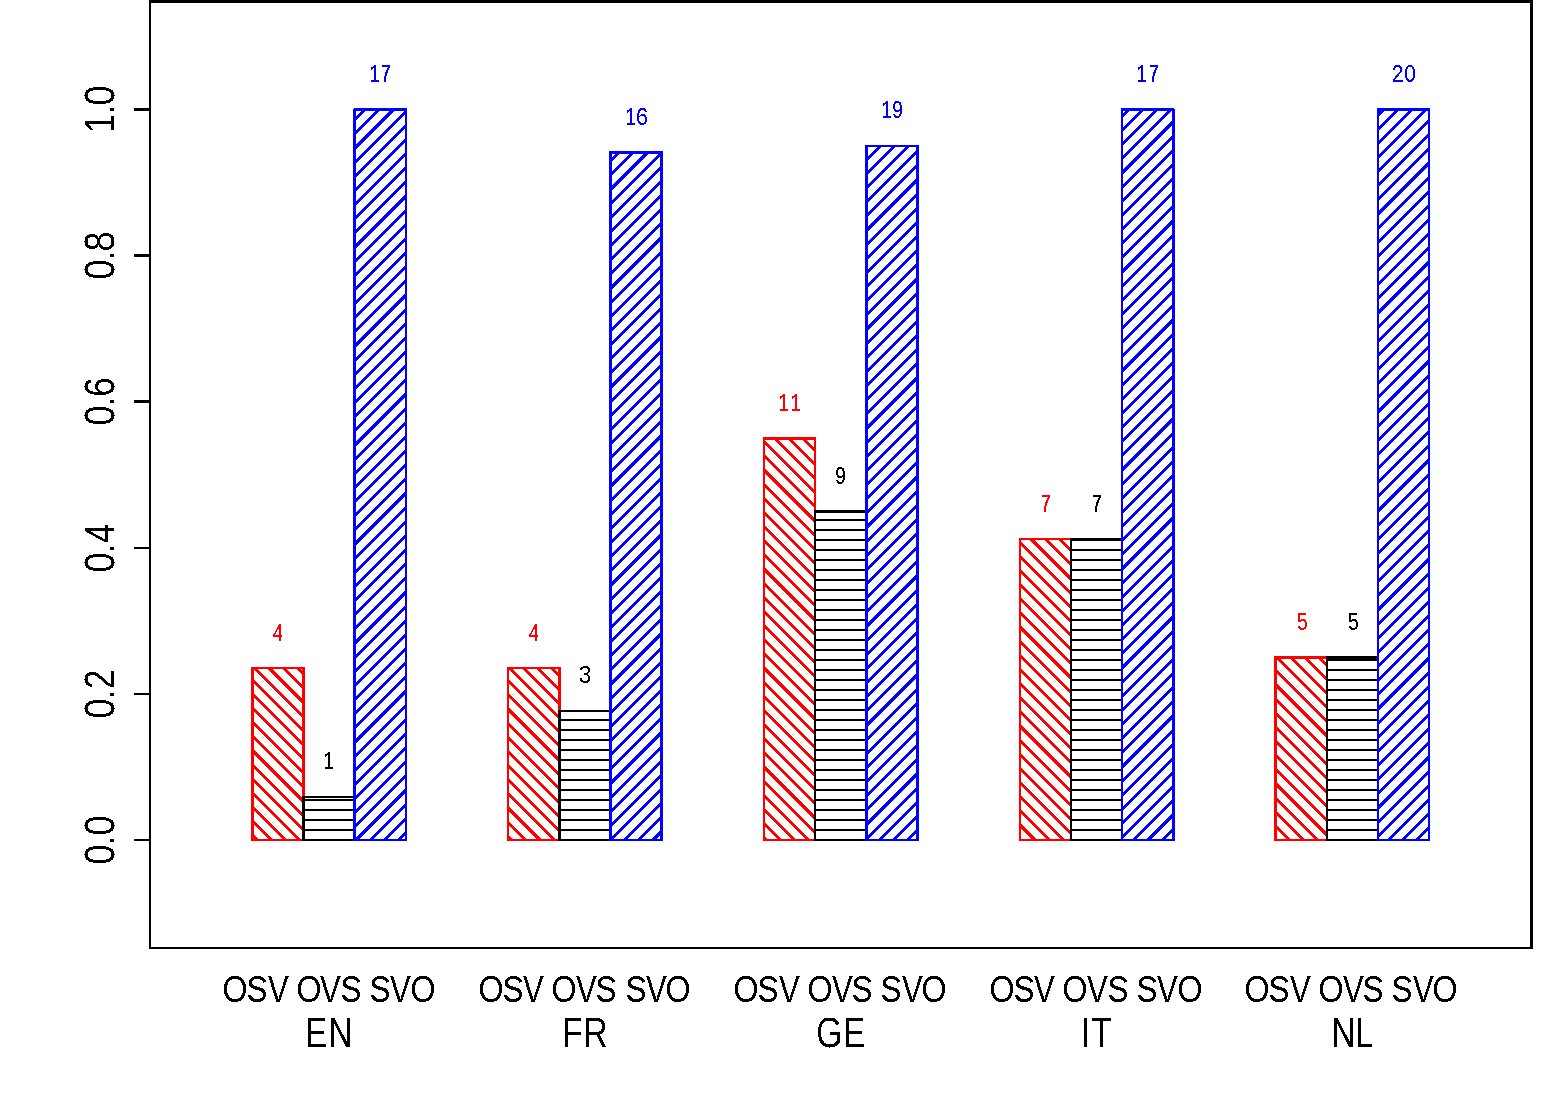
\includegraphics[width=\textwidth]{figures/05-5.pdf}
    \caption{Comprehension task, learner above chance}
    \label{fig:05:5}
\end{figure}

The first noteworthy observation concerns the obvious difference between the processing of SO targets, on the one hand, and of OS ones, on the other hand. It is curious that two learners (one German, one French) did not achieve above-chance accuracy on this type of targets. 

Nevertheless, quite a few participants seemed able to correctly process OS targets: this regards 31 learners on OSV and 25 on OVS targets. All L1s are represented, although values for the Italian and German groups are higher than others. 

The two values of OS (OSV and OVS) appear to be very similar. If a difference exists, it is very slight and in favour of OSV. 

\figref{fig:05:6} presents the data at T2.

\begin{figure}
    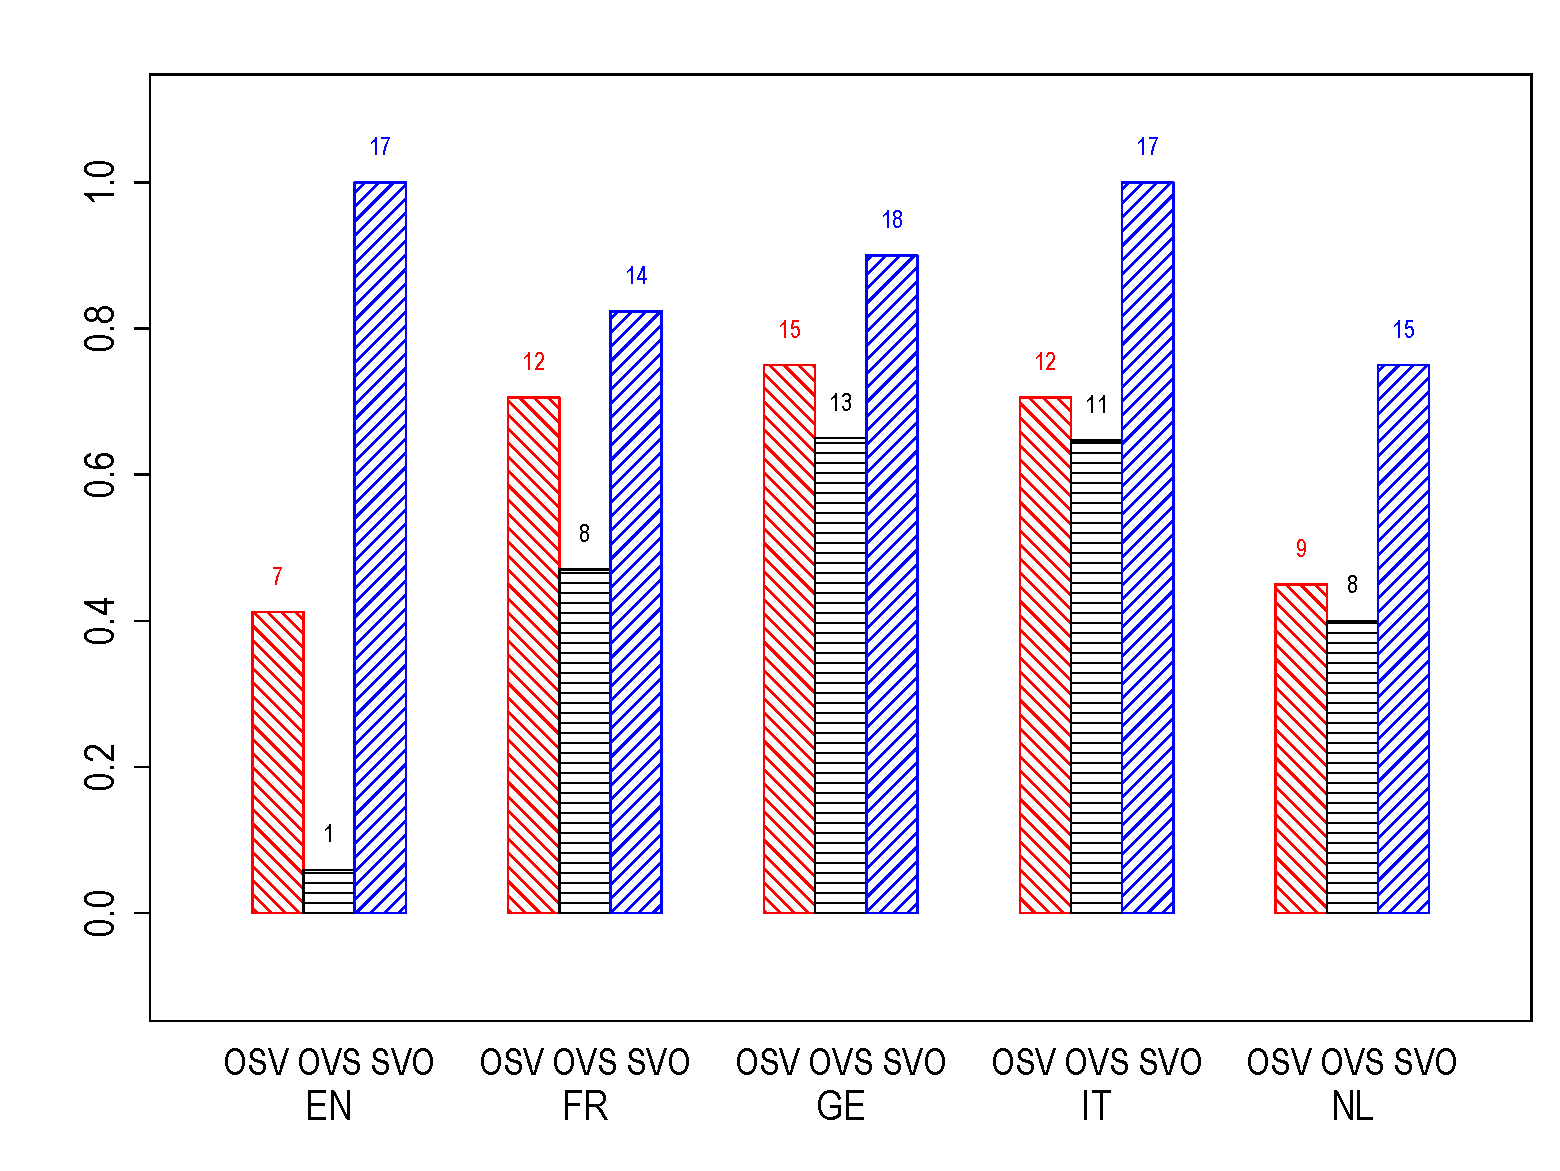
\includegraphics[width=\textwidth]{figures/05-6.pdf}
    \caption{Learners significantly above chance by L1, comprehension task}
    \label{fig:05:6}
\end{figure}

Two main tendencies can be observed. The first concerns the marked increase in the number of learners with above-chance accuracy in the processing of OS targets, which grows in all L1 groups. With the only exception of the L1 English group, the improvement concerns both values of OS, although the advantage of OSV over OVS remains. Although less evidently than at T1, the L1 Italian and L1 German groups still achieve better performance than the other groups.

Second, the number of learners failing to reach above-chance accuracy on SO also increases.

\subsection{A comprehensive picture}\label{sec:05:2.4}

Data can also be displayed so that the scores of each individual learner may be synoptically seen as a function of L1, word order, and time. The objective is to perform a simple cluster analysis to verify whether learners can be grouped based on these factors. 

In \figref{fig:05:3}, T1 and T2 scores are presented on the horizontal (black) and on the vertical (red) axis, respectively. On both axes, scores are defined by the combination of learner performance on the three target word orders: SVO, OVS and OSV. A score of 1 indicates that the learner performs above chance on the corresponding target structure, whereas 0 indicates a chance-level response.

Learners are thus identified by a combination of scores at T1 (horizontal axis, black) and T2 (vertical axis, red), that is, by their position in one of the 64 squares in which the graph area is divided. Each data point represents an individual learner, whose L1 is also specified.

\begin{figure}
    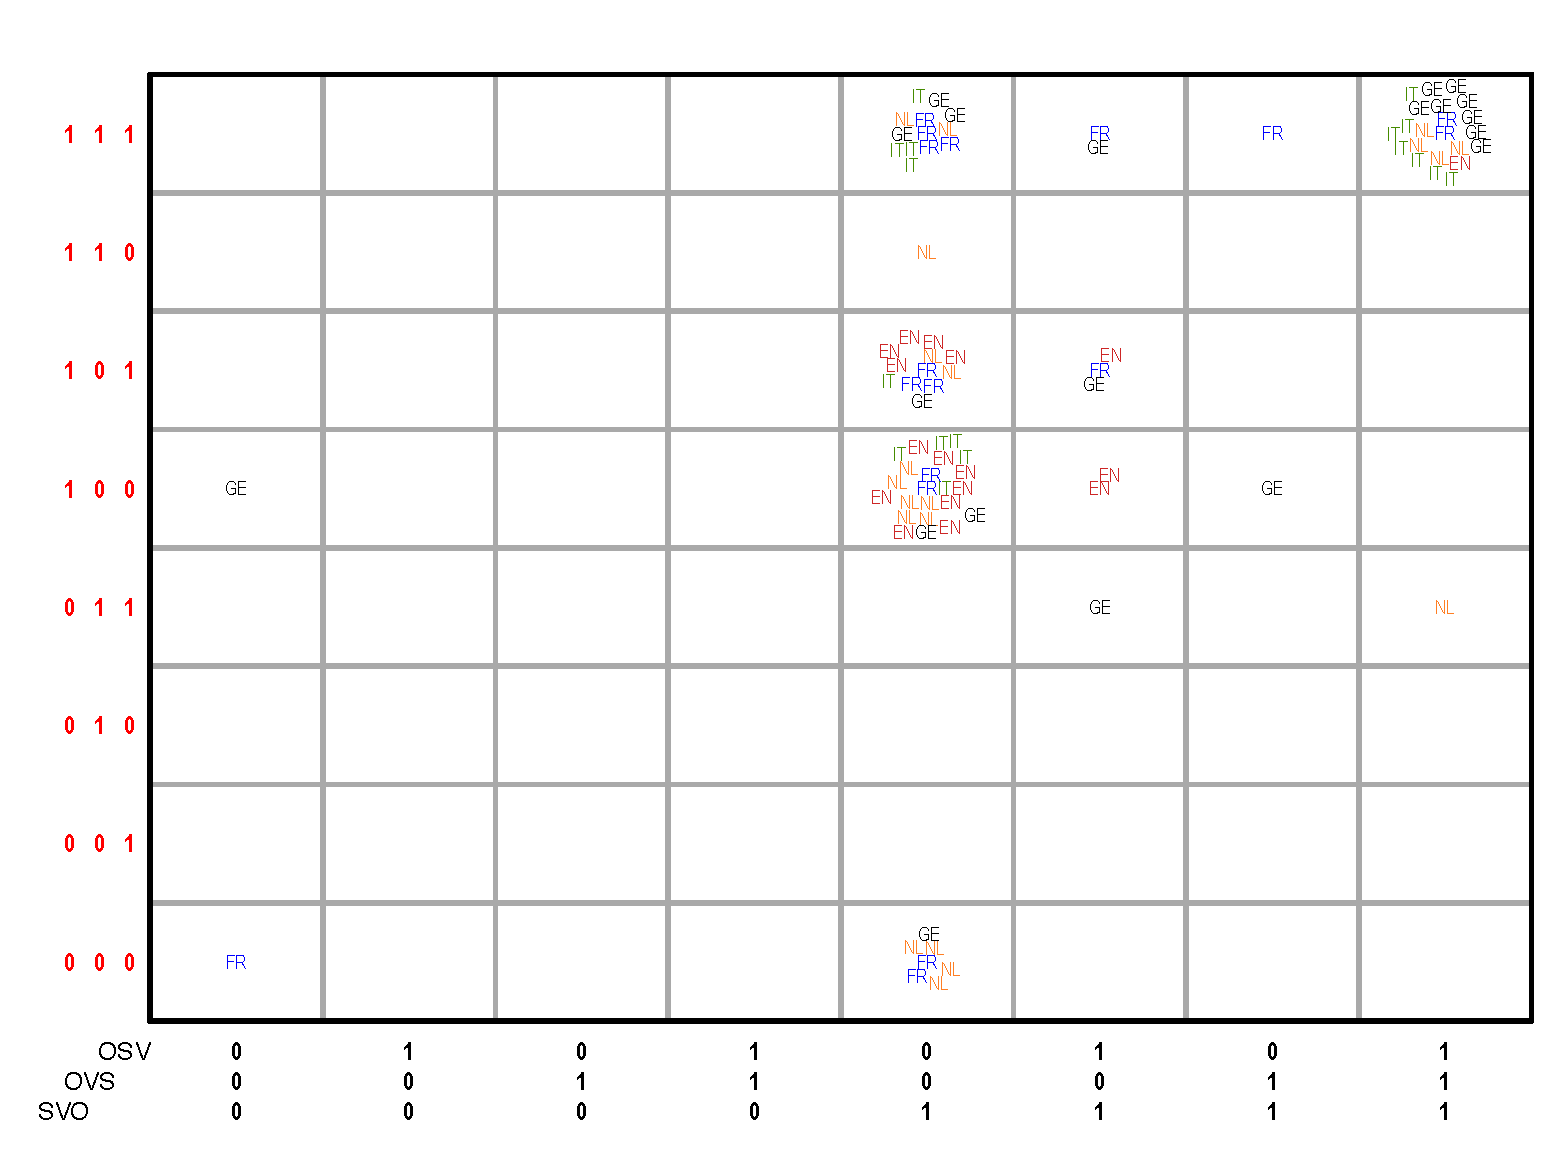
\includegraphics[width=\textwidth]{figures/05-7.pdf}
    \caption{Comprehension task, individual processing strategies}
    \label{fig:05:7}
\end{figure}

Out of the 64 theoretically possible scenarios, only a few are realised in practice, and fewer still include the bulk of the subjects. As each square corresponds to a varying degree of success in the test, i.e. on various types of targets, one could interpret this information as a hint to the existence of a hierarchy in the development of morphosyntactic competence in comprehension, identifiable both synchronically and diachronically. For a synchronic analysis, one needs to consider the column sum, for T1, or the row sum, for T2, in order to compute the number of participants performing in a specific manner at either test time. 

At T1, most learners (56) show the following score: SVO 1, OVS 0, OSV 0, which corresponds to a clear positional strategy. 23 learners, in contrast, already exhibit a well-developed morphosyntactic strategy (SVO 1, OVS 1, OSV 1). In between these two groups, 8 learners correctly process SVO and OSV targets, but not OVS, and only 2 do the opposite, which suggests that OSV structures should be more accessible compared to their OVS equivalents. 

At T2, the number of learners applying a pure positional principle (fourth line in the graph) is reduced to 26, whereas those always using a morphosyntactic strategy (first line) are now 36. 15 participants, finally, perform better on OSV than OVS targets. The picture at T2, therefore, confirms the situation at T1, with a tendency for results to become more target-like.

One can also study the evolution of learners' processing strategies over time. It seems most relevant to describe the potential evolution of the 56 participants who at T1 were found to adopt a pure positional strategy (SVO 1, OVS 0, OSV 0). 23 of them did not change their processing strategy, consistently applying the same strategy at T2 as well. In contrast, 13 participants moved all the way towards a morphosyntactic strategy, so that at T2 they proved able to consistently derive meaning from both SO and OS targets. 12 learnt to process OSV structures, but still not OVS; only 1 learner exhibits the reverse evolution. This information fits in with the synchronic data, which showed that at both T1 and T2 OSV targets are correctly processed by a greater number of learners than their OVS equivalents. Diachronically, it appears that case marking in the two OS word orders can develop either at same time, or separately, in which case OSV develops first. 

Finally, 7 subjects (last line, fifth column) move to a stage in which no word order is processed with  above- chance accuracy. Beside the fact that additional exposure to the input is apparently detrimental to these learners, this last scenario is particularly surprising in light of the fact that the meaning of SO targets can be correctly identified based on a positional principle.

\subsection{Differential processing of OS word orders}\label{sec:05:2.5}

The analysis so far has revealed obvious gaps in scores between SO targets, on the one hand, and OS targets, on the other hand. These differences are not problematic in that they can easily be explained by the processing principle required to extract meaning from them: positional or morphosyntactic in the former case, necessarily morphosyntactic in the latter. When it comes to OS targets, however, there should be no differences in processing accuracy, as both OSV and OVS targets share the same relative order of subject and object. Nevertheless, it does seem that OVS targets prove consistently harder to process than OSV ones. Evidence for such claim comes from various sources: alongside marked differences in mean scores, the processing of OVS targets was often found not to reach above-chance performance; further, scenarios in which, at a given time, OVS structures are processed more accurately than OSV are rare; diachronically, OSV almost always develops before OVS. This section first describes the phenomenon in detail and then reports on a statistical test to verify whether the observed differences are statistically significant and require a specific explanation.

\figref{fig:05:4} presents an overall picture of each learner's processing strategy of OS targets at both T1 and T2. The processing scores of OSV targets are represented on the horizontal axis, with learners behaving at chance level on the left (scenarios 2 and 4), and learners above chance on the right (scenarios 1 and 3). Conversely, the processing scores of OVS targets are represented on the vertical axis, with learners behaving at chance level at the bottom (scenarios 2 and 3) and learners above chance at the top (scenarios 2 and 4). Taken together, the two scores provide an overall picture of learners' behaviour on both OVS and OSV targets at the same time. The main area is divided into four main squares, each representing a processing scenario at T1 according to the conventions summarised in \tabref{tab:05:6}.

\begin{table}
    \begin{tabular}{|lc|cc|}
    \hline
    & & \multicolumn{2}{c|}{OSV}\\
    &  & p ${\leq}$ 0.05 & p $>$ 0.05\\
    \hline
    \multirow{2}{*}{OVS} & p ${\leq}$ 0.05 & 1 & 4\\
                         & p $>$ 0.05 & 3 & 2\\
    \hline
    \end{tabular}
    \caption{Scenarios, rationale}
    \label{tab:05:6}
\end{table}

Scenario 1 indicates that the learner processes both OSV targets (horizontal axis, black) and OVS targets (vertical axis, red), based on a morphosyntactic principle whereby the first NP is always interpreted as the subject. Scenario 2 is the reverse, that is, both types of target are processed positionally, which leads to an incorrect interpretation of the sentence. In scenario 3, OSV targets are processed in a target-like manner, whereas OVS targets are not; the opposite happens in scenario 4. The last two scenarios are particularly relevant for the present research question, as they suggest a discrepancy in the processing of the two types of OS target.

The main squares are further divided into four smaller squares each, which represent the same processing scenarios, in the same order, but relative to T2. In this manner, an indication of the evolution in time of learner processing strategies is included in the graph. Overall scenarios are identified by the two digits corresponding to learner performance at T1 and T2, in that order.

\begin{figure}
    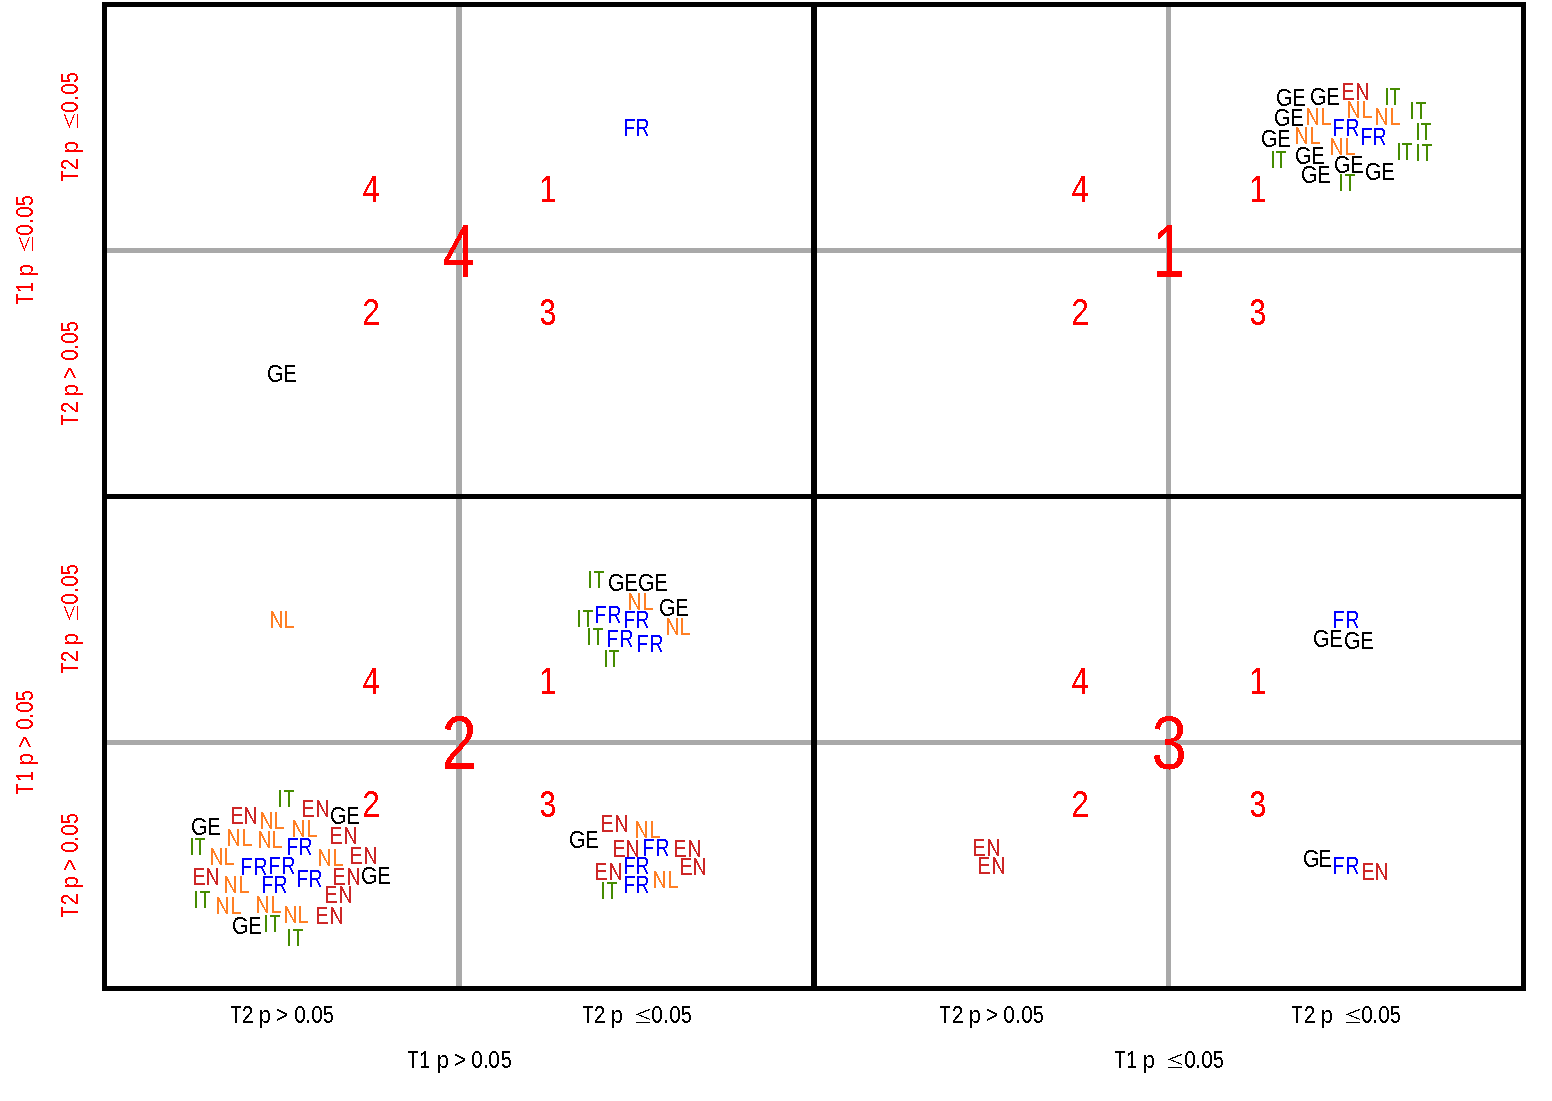
\includegraphics[width=\textwidth]{figures/05-8.pdf}
    \caption{Comprehension task, individual processing strategies, OSV-OVS targets}
    \label{fig:05:8}
\end{figure}

The two main clusters which can be identified concentrate in scenarios 2;2 and 1;1, both representing an extreme picture. In scenario 2;2, learners consistently process both types of OS targets based on a positional principle. Their situation is stable between T1 and T2. 

Conversely, learners in scenario 1;1 apply a target-like morphosyntactic strategy at both test times. 

Two further major clusters originate from scenario 2 at T1, which indicates a positional principle on both types of targets at T1. However, these learners evolve differently with time: those in scenario 2;1 move on to scenario 1 at T2, which means that over time they learnt to generalise a morphosyntactic strategy to all OS targets. Those in scenario 2;3 managed to do so only on OSV targets, and not on OVS ones. The reverse situation, with learners processing correctly OVS targets, but not OSV ones, is only instantiated by a single learner. This suggests that in diachrony, OSV targets tend to be acquired first.

Synchronically, more learners appear in scenario 3 than in scenario 4 at both T1 and T2, as shown in \tabref{tab:05:7} and \ref{tab:05:8} respectively.

\begin{table}
    \begin{tabular}{|lc|cc|}
    \hline
    & & \multicolumn{2}{c|}{OSV}\\
    &  & p ${\leq}$ 0.05 & p $>$ 0.05\\
    \hline
    \multirow{2}{*}{OVS} & p ${\leq}$ 0.05 & 23 & 2\\
    & p $>$ 0.05 & 8 & 58\\
    \hline
    \end{tabular}
    \caption{Comprehension test, OS targets, learner distribution across scenarios, T1}
    \label{tab:05:7}
\end{table}

\begin{table}
    \begin{tabular}{|lc|cc|}
    \hline
    & & \multicolumn{2}{c|}{OSV}\\
    &  & p ${\leq}$ 0.05 & p $>$ 0.05\\
    \hline
    \multirow{2}{*}{OVS}& p ${\leq}$ 0.05 & 40 & 1\\
    & p $>$ 0.05 & 15 & 35\\
    \hline
    \end{tabular}
    \caption{Comprehension test, OS targets, learner distribution across scenarios, T2}
    \label{tab:05:8}
\end{table}

It thus appears that OSV targets are indeed easier to process than OVS; in the following lines a few reasons for this will be explored. In SVO targets \REF{ex:05:1}, agent and patient appear in utterance-initial and utterance-final position respectively, whereas the verb is in utterance-medial position. As SVO is the dominant order in both the target language and the learners' L1s, this structure may be considered to be the prototype of transitive utterances. 

\ea%1
    \label{ex:05:1}
    \gll    {siostr-a}   {woła}   {brat-a}\\
            sister-\textsc{nom}   calls  brother-\textsc{acc}\\
    \glt    `(The) sister calls (her) brother.'
    \z

OVS targets also present the two nouns in utterance-initial and utterance-final position and the verb in utterance-medial position: this time, however, the patient comes first. This structure is therefore identical to SVO as far as the relative order of phrases is concerned. The only way to correctly process this type of targets, or to distinguish them from their SVO equivalents, is to process inflectional morphology.  

\ea%2
    \label{ex:05:2}
    \gll    {brat-a}     {woła}  {siostr-a}\\
            brother-\textsc{acc}  calls  sister-\textsc{nom}\\
    \glt    `(The) sister calls (her) brother.'
    \z

Morphosyntactic processing requires learners to be aware of the gender and inflectional class of target nouns: as \REF{ex:05:2} makes it clear, both nouns may be marked by the same ending, whose meaning (\textsc{nom.sg.f} vs. \textsc{acc.sg.m}) depends on the paradigm to which the noun belongs. Combined with the modest prominence of case endings and the pressure exerted by the test, this may confuse learners, leading them to mistake these targets for instances of SVO utterances. In other words, it may be the case that whenever learners encounter a sentence with the structure NP — V — NP, they interpret it as SVO. It may not be a chance that this tendency is particularly strong with English and French learners, that is, speakers of languages whose word order is particularly rigid, which in turn leads to a very stringent association between the linear order of phrases and meaning.

The picture changes with OSV targets \REF{ex:05:3}, in which the structure of the utterance is quite different: the two noun phrases come first, followed by the verb. This order hardly ever appears in the input, and is therefore unfamiliar to the learners. This seems to be enough for them to notice the difference from the prototype, rather marked in fact, and pay attention to inflectional morphology, or perhaps interpret the utterance as OS simply because it appears so different from the prototypical SVO structure. 

\ea%3
    \label{ex:05:3}
    \gll    {brat-a}     {siostr-a}   {woła}\\
            brother-\textsc{acc}  sister-\textsc{nom}  calls\\
    \glt    `(The) sister calls (her) brother.'
    \z

\subsubsection{Differential processing of OS word orders: Inferential statistics}\label{sec:05:2.5.1}

To test the effect of OS word order statistically, the generalised linear mixed model described in \sectref{sec:05:2.1} was compared to an identical model, in which, however, the predictor WO2 (word order with two values, i.e. SO and OS) was substituted with the predictor WO3 (word order with three values, i.e. SVO, OVS and OSV). The model output is presented in \tabref{tab:05:9}.

\begin{table}
    \begin{tabularx}{\textwidth}{Xrrr}
    \lsptoprule
    \textit{predictors} & \textit{odds} \textit{ratios} & \textit{CI} & \textit{p}\\
    \midrule
    (intercept) & 0.28 & 0.07~—~1.09 & 0.067\\
    time [2] & 4.15 & 0.99~—~17.38 & 0.051\\
    L1 [FR] & 2.33 & 0.38~—~14.30 & 0.360\\
    L1 [GE] & 17.70 & 2.96~—~105.90 & \textbf{0.002}\\
    L1 [IT] & 4.08 & 0.61~—~27.20 & 0.146\\
    L1 [NL] & 1.43 & 0.24~—~8.67 & 0.696\\
    WO3 [OVS] & 0.01 & 0.00~—~0.04 & \textbf{<0.001}\\
    WO3 [SVO] & 681.07 & 111.54~—~4158.79 & \textbf{<0.001}\\
    time [2] * L1 [FR] & 2.52 & 0.34~—~18.69 & 0.367\\
    time [2] * L1 [GE] & 1.31 & 0.18~—~9.44 & 0.787\\
    time [2] * L1 [IT] & 3.28 & 0.38~—~28.23 & 0.280\\
    time [2] * L1 [NL] & 1.18 & 0.16~—~8.65 & 0.872\\
    time [2] * WO3 [OVS] & 1.37 & 0.73~—~2.58 & 0.324\\
    time [2] * WO3 [SVO] & 0.41 & 0.19~—~0.91 & \textbf{0.028}\\
    L1 [FR] * WO3 [OVS] & 31.41 & 4.97~—~198.62 & \textbf{<0.001}\\
    L1 [GE] * WO3 [OVS] & 117.22 & 17.14~—~801.53 & \textbf{<0.001}\\
    L1 [IT] * WO3 [OVS] & 94.50 & 11.59~—~770.64 & \textbf{<0.001}\\
    L1 [NL] * WO3 [OVS] & 37.62 & 5.60~—~252.89 & \textbf{<0.001}\\
    L1 [FR] * WO3 [SVO] & 0.04 & 0.00~—~0.31 & \textbf{0.002}\\
    L1 [GE] * WO3 [SVO] & 0.00 & 0.00~—~0.03 & \textbf{<0.001}\\
    L1 [IT] * WO3 [SVO] & 0.16 & 0.02~—~1.66 & 0.124\\
    L1 [NL] * WO3 [SVO] & 0.19 & 0.02~—~1.61 & 0.129\\
    \multicolumn{4}{c}{\textbf{random} \textbf{effects}}\\
    σ\textsuperscript{2} & \multicolumn{3}{r}{3.29}\\
    τ\textsubscript{00}~\textsubscript{participant} & \multicolumn{3}{r}{6.15}\\
    τ\textsubscript{00}~\textsubscript{target\_no} & \multicolumn{3}{r}{0.24}\\
    τ\textsubscript{11}~\textsubscript{participant.time2} & \multicolumn{3}{r}{6.63}\\
    τ\textsubscript{11}~\textsubscript{participant.WO3OVS} & \multicolumn{3}{r}{3.83}\\
    τ\textsubscript{11}~\textsubscript{participant.WO3SVO} & \multicolumn{3}{r}{5.19}\\
    ρ\textsubscript{01}~\textsubscript{participant.time2} & \multicolumn{3}{r}{{}-0.14}\\
    ρ\textsubscript{01}~\textsubscript{participant.WO3OVS} & \multicolumn{3}{r}{0.70}\\
    ρ\textsubscript{01}~\textsubscript{participant.WO3SVO} & \multicolumn{3}{r}{{}-0.91}\\
    ICC & \multicolumn{3}{r}{0.76}\\
    N~\textsubscript{participant} & \multicolumn{3}{r}{91}\\
    N~\textsubscript{target\_no} & \multicolumn{3}{r}{24}\\
    observations & \multicolumn{3}{r}{4248}\\
    marginal R\textsuperscript{2}~/ conditional R\textsuperscript{2} & \multicolumn{3}{r}{0.375 / 0.852}\\
    \lspbottomrule
    \end{tabularx}
    \caption{Model output}
    \label{tab:05:9}
\end{table}

A likelihood-ratio test reveals a statistically significant difference between the two models (Chisq = 131.41, Df = 10, p < 0.01), which suggests that accounting for the differential processing of OS word order configuration is beneficial to the interpretation of the data. However, pairwise comparisons (\figref{fig:05:9}) reveal that the difference in score between the processing of OVS and OSV is significant only for L1 English learners (p < 0.01 at both test times).

\begin{figure}
    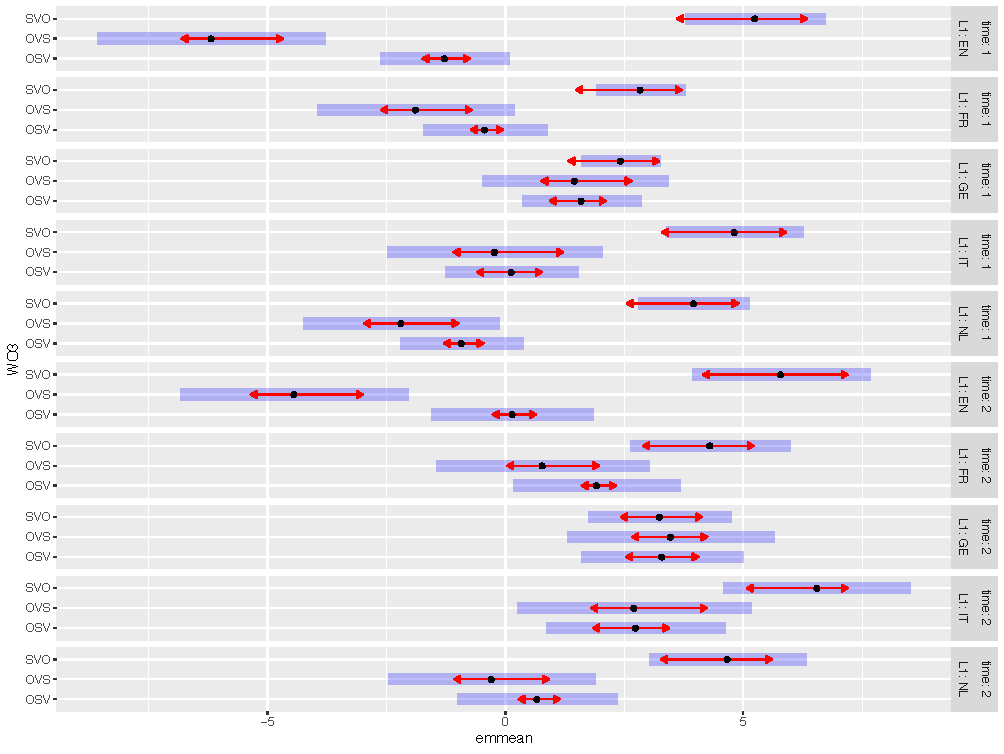
\includegraphics[width=\textwidth]{figures/05-9.pdf}
    \caption{Pairwise comparisons, WO3 across L1 and time}
    \label{fig:05:9}
\end{figure}

\section{Summary}\label{sec:05:3}

This chapter described the results of the Comprehension test, in which learners were asked to listen to a short transitive utterance and to identify its syntactic structure by selecting the appropriate picture. The main findings can be summarised as follows. First, as hypothesised, SO structures are more easily interpreted than their OS equivalent. Second, the learners' familiarity with OS targets increases with time, so that, by T2, a fair half of the subjects can consistently process all target structures. Finally, all L1 groups behave in a comparatively similar manner with the only exception of the English learners, who appear to be much more biased towards an agent-first interpretation of any target structure.

\chapter{A Comprehensive View of Morphosyntactic Skills}

\section{Research questions and hypotheses}\label{sec:06:1}

The purpose of this chapter is to verify to what extent the VILLA learners acquired a morphosyntactic principle of utterance organisation, whereby grammatical meaning is encoded by inflectional morphology independently of word order. To this purpose, the results of the EI task (chapter 3) and of the comprehension test (chapter 4) are correlated, arguing that "validation studies are fundamentally based on the “triangulation” of various methods. The fact that a structure has emerged could thus be demonstrated on the basis of several elicitation procedures […]" \citep[326]{Pallotti2006}\todo{Do you mean \citet{Pallotti2007}. If not, this is missing from the bibliography.}. The present analysis aims to verify whether the target structure is simultaneously mastered in both comprehension and repetition, or if it develops in either of them first, in either SO or OS word order. The effect of other predictors such as input exposure and L1 is also investigated.

\subsection{Task type}\label{sec:06:1.1}

The EI task requires learners to phonologically decode, and possibly comprehend, the target sentence and then reproduce it based on their interlanguage grammar. In a sense, it should in principle, encompass the same skills needed for the comprehension test, although there are some important differences. The first is that repetition may take place without comprehension, although the task was designed so as to make this unlikely. Secondly, repetition involves a further skill, that is, language production, and it may therefore be argued that it represents a more complex task comprising several skills at the same time. For this reason it is expected that it will produce poorer results, i.e. some learners may be able to process a given target in comprehension, but not in repetition.

\subsection{Word order}\label{sec:06:1.2}

As has been argued in chapters 4 and 5, the effects of word order differ in the two tasks at hand. In the comprehension test, word order directly correlates with markedness, as SO targets conform to the first-noun principle while OS targets violate it. The picture is more complex in the case of the EI task (see section SECTION\todo{To be updated}), but in short it can be said that OS targets should prove harder for the following reasons: a) OS violates the first-noun principle; b) when producing OS structures, the non-nominative case ending must be supplied outside its canonical position, which, in initial interlanguages, is typically post-verbal; c) the non-nominative case ending occurs in the perceptually non-salient utterance-medial position. 

It is thus expected that results on OS targets will be poorer in both tests.

\subsection{Correlation between task type and word order}\label{sec:06:1.3}

The overall purpose of this chapter is to identify the contexts in which learners can be hypothesised to adopt a morphosyntactic principle, “context” referring to a combination of task type and target sentence word order (e.g. repetition of OS targets). Further, it may be the case that, in order to master one particular context, learners must be able to develop others first (e.g. the comprehension of OS targets and the repetition of SO targets). The analysis thus aims to identify possible implications between contexts (e.g. the repetition of OS targets implicating their comprehension), in order to identify a difficulty scale. 

\subsection{Cross-linguistic influence}\label{sec:06:1.4}

It is expected that speakers of languages with relatively free word order and case marking should be favoured. Within the VILLA project only German possesses such characteristics, albeit to a more limited extent that Polish. Rigid word order as observed in English and French is hypothesised to impose a positional principle on the learner, thus slowing down the acquisition of the target structure. L1 biases may also prompt learners who are not familiar with the category of case to rely on information such as animacy and word order to identify the agent of the sentence. These cues are admittedly relevant in the processing of many Polish real-life utterances, but were purposefully excluded in the present experimental paradigm.

\subsection{Exposure to the input}\label{sec:06:1.5}

Intuitively, additional exposure to the input can only be beneficial for the acquisition of the target structure. In addition, two more specific questions may be formulated. 

\begin{itemize}
    \item Implicational sequence of development. Improving in one context may require learners to master others first, according to the implicational scale hypothesised in 1.2.3\todo{Section?}. This requires that the implicated abilities should be already developed at T1, or develop between the two test times. It is predicted that learners will improve in comprehension before repetition, and on SO targets before OS ones.
    \item Cross-linguistic differences. This question regards the presence of interactions between a possible implicational scale of development and the learners' L1. It may be the case, for instance, that speakers of a certain L1 improve on particular combination of task type and word order. Participants advantaged by their L1 from a cross-sectional perspective should also exhibit faster and more significant gains.
\end{itemize}

\section{The comprehension test as a disambiguator to the EI task}\label{sec:06:2}

The comprehension test can be helpful to shed light on some of the questions which emerged from the analysis of the EI task. Given a repeated utterance like \REF{ex:06:1}, it is impossible to establish \textit{a priori} whether or not the learner truly attempted to encode any specific meaning, and, if so, what this may be. 

\ea%1
    \label{ex:06:1}
    \gll    [artɨstk-a  pozdravja  twumaʧk-a]\\
            artist-\textsc{nom}  cheers    interpreter-\textsc{nom}\\
    \z

The question is particularly relevant in the case of OS targets. Learners may fail not only on the repetition of the non-basic ACC ending, but also on the comprehension of the target sentence, which, according to the first-noun principle, could be processed as a default subject-initial utterance. With regard to a target utterance like \REF{ex:06:2}: 

\ea%2
    \label{ex:06:2}
    \gll    /arˈtɨstk-e  pozˈdravja  twuˈmaʧk-a/\\
            artist-\textsc{acc}  cheers    interpreter-\textsc{nom}\\
    \glt    `The interpreter cheers the artist.'
    \z

An output like \REF{ex:06:1} may instantiate at least three underlying structures \REF{ex:06:3}:

\ea%3
    \label{ex:06:3}
    \ea\label{ex:06:3a}
    artist-\textsc{obj}  cheers    interpreter-\textsc{subj}
    \ex\label{ex:06:3b}
    artist-\textsc{subj}  cheers    interpreter-\textsc{obj}
    \ex\label{ex:06:3c}
    artist     cheer    interpreter
    \z
\z

\REF{ex:06:3a} corresponds to target-like comprehension of the OS target, the deviant output in \REF{ex:06:1} owing to a failure to \textit{produce} a non-basic word-form, which nonetheless was correctly identified in comprehension. In \REF{ex:06:3b}, the utterance is interpreted as subject initial based on a positional principle and in spite of inflectional morphology. In \REF{ex:06:3c}, finally, the learner only identifies lexical items with no attached grammatical meaning. In the latter case, the learner is not reproducing a sentence, but rather a list of words with no meaningful connection.

In the absence of a translation test, output like \REF{ex:06:1} is bound to remain ambiguous. The comprehension test makes it possible to reduce the degree of uncertainty concerning the learner’s underlying structures as exemplified in \REF{ex:06:3}. Should the comprehension test show that a particular learner is incapable of processing OS targets, then it would be highly unlikely that the same learner could have processed the same target correctly in the EI task. At most, the learner might have attempted to encode a SO utterance, so that the source of incorrect output lies in comprehension: one could thus exclude option \REF{ex:06:3a}. If a learner performs above chance on the comprehension test, in contrast, the possibility exists that he might have tried to produce an OS utterance, though failing to encode grammatical meaning through case endings. The difficulty in this case should be localised at the level of repetition, rather than comprehension.

To summarise, correlating the two tests cannot provide final answers as to the learner's strategies of utterance organisation, but makes it possible to exclude unlikely explanations of the observed output.

\subsection{Correlating the repetition and comprehension tests: methodology}\label{sec:06:2.1}

In order to correlate the results of the repetition and the comprehension tests, a first intuitive approach might be plotting the learners' scores in various test conditions (task, word order, time) side by side, as in histograms or boxplots like \figref{fig:06:1}. However, with this approach, it is impossible to trace the behaviour of individual participants across various conditions, as is indeed the purpose in the present work, because individual learners are not univocally identified. To exemplify, it is impossible to tell how the single participant scoring just below 0.8 in the comprehension of SO targets performed in the other conditions.

\begin{figure}
    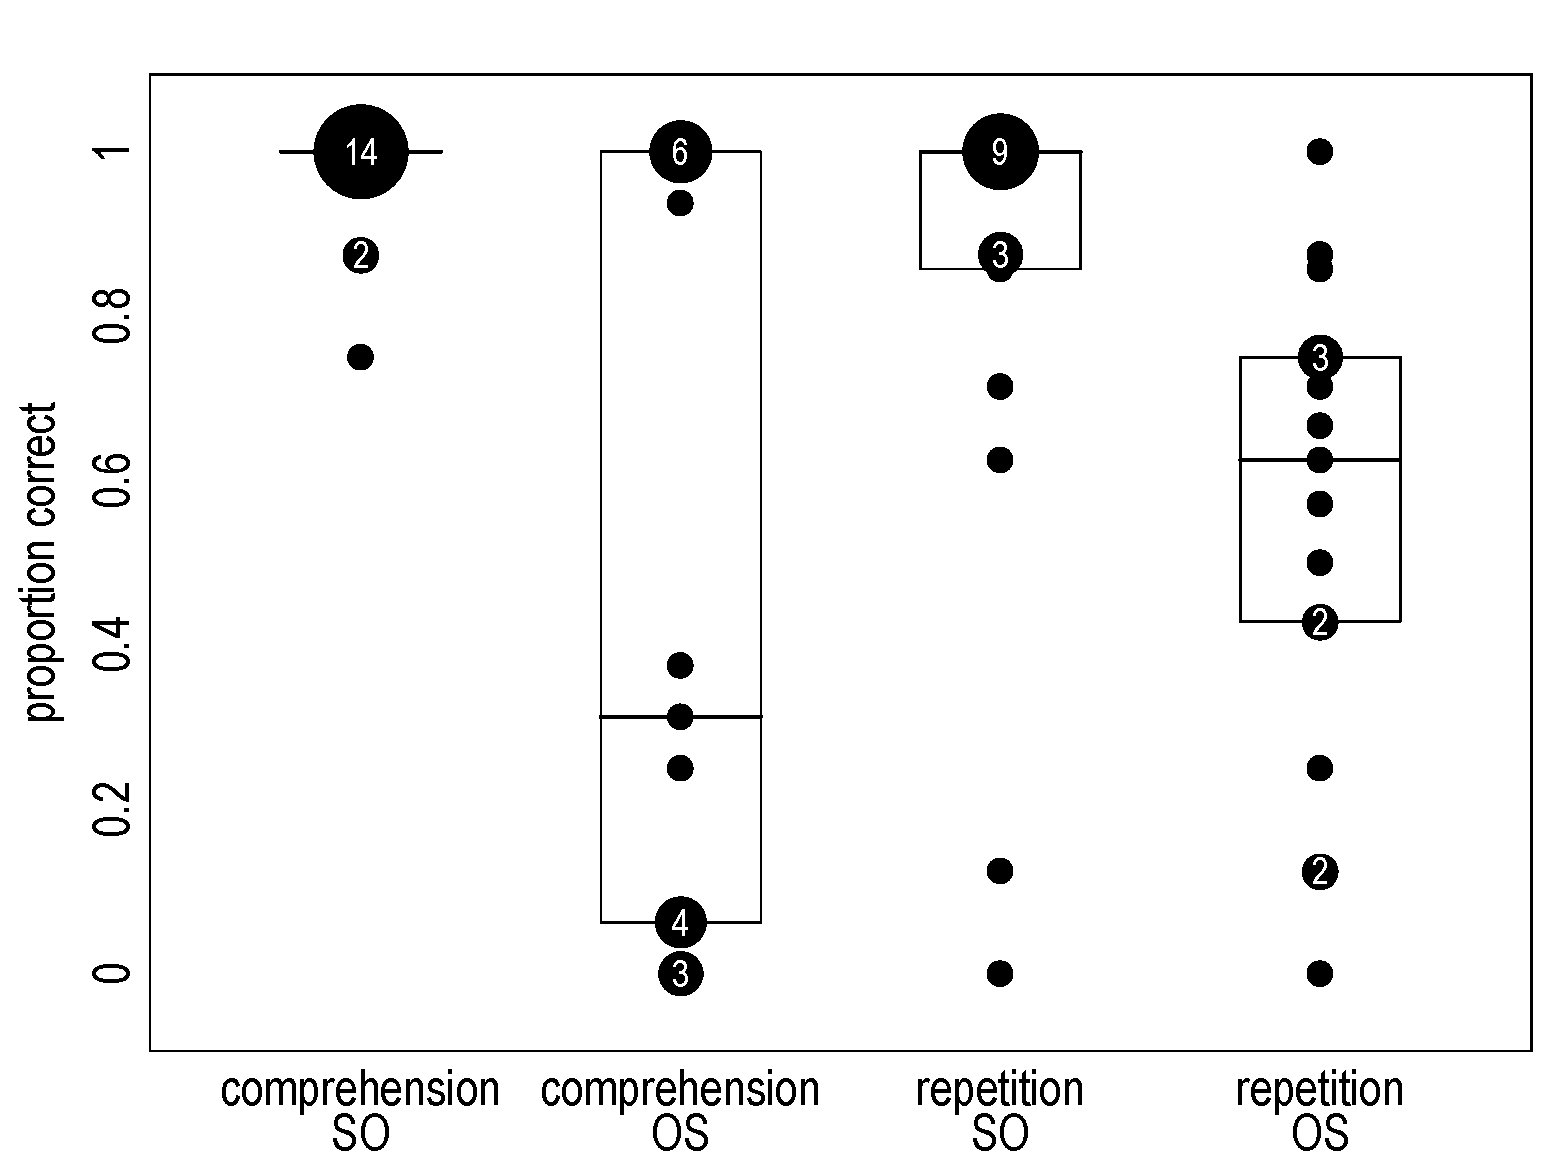
\includegraphics[width=\textwidth]{figures/06-1.pdf}
    \caption{Italian learners’ performance at T1, comprehension test and EIT}
    \label{fig:06:1}
\end{figure}

Moreover, differences in aggregated scores, even if proved to be statistically significant, do not necessarily have a linguistic interpretation. Finally, each graph only describes the performance of a single L1 group at either test time. In the case of a complex project such as VILLA, it would take ten such graphs to fully describe tendencies in the data-set.

To address this first limitation, \tabref{tab:06:1} presents the proportion of learners scoring statistically above chance in each test condition, based on the methodology described in section \ref{sec:04:2.4}. 

\begin{table}
    \begin{tabularx}{\textwidth}{XXXXXXXXXXXXXXXXX} & \multicolumn{8}{X}{ OS} & \multicolumn{8}{X}{ SO}\\
    \lsptoprule
    & \multicolumn{4}{X}{ T1} & \multicolumn{4}{X}{ T2} & \multicolumn{4}{X}{ T1} & \multicolumn{4}{X}{ T2}\\
    & \multicolumn{2}{X}{ Comp} & \multicolumn{2}{X}{ EI} & \multicolumn{2}{X}{ Comp} & \multicolumn{2}{X}{ EI} & \multicolumn{2}{X}{ Comp} & \multicolumn{2}{X}{ EI} & \multicolumn{2}{X}{ Comp} & \multicolumn{2}{X}{ EI}\\
    & + & {}- & + & {}- & + & {}- & + & {}- & + & {}- & + & {}- & + & {}- & + & {}-\\
    EN & 1 & 16 & 0 & 17 & 1 & 16 & 0 & 17 & 17 & 0 & 0 & 16 & 16 & 0 & 0 & 16\\
    FR & 4 & 13 & 0 & 17 & 9 & 8 & 2 & 15 & 16 & 1 & 1 & 16 & 14 & 3 & 5 & 12\\
    GE & 10 & 7 & 7 & 13 & 15 & 5 & 11 & 9 & 19 & 1 & 8 & 12 & 18 & 2 & 9 & 11\\
    IT & 7 & 10 & 6 & 11 & 11 & 6 & 8 & 9 & 17 & 0 & 13 & 4 & 17 & 0 & 14 & 3\\
    NL & 5 & 15 & 2 & 18 & 8 & 12 & 5 & 15 & 20 & 0 & 6 & 14 & 15 & 5 & 7 & 13\\
    \lspbottomrule
    \end{tabularx}
    \caption{Learners scoring above chance}
    \label{tab:06:1}
\end{table}

This time the data are arranged and interpreted in such a way that they have an immediate linguistic interpretation, that is, whether or not the learners can be thought to have applied a morphosyntactic strategy. Again, however, no information is provided as to the score of individual learners in various conditions.

\subsection{Scenarios}\label{sec:06:2.2}

In order to portray a comprehensive picture of learners’ morphosyntactic skills, “scenarios” (see section \ref{sec:04:2.4.3}\todo{No 2.4.3 in Chapter 4; only 2.4 and 2.4.1}) are introduced as a methodological tool. Scenarios represent a single, global score of the learners' processing skills in both comprehension and repetition. For each test, scores are coded as 'positive' or ‘negative’ based on the rationale described in section (SECTION)\todo{To be updated}. Four scenarios are possible (\tabref{tab:06:2}):

\begin{table}
    \begin{tabularx}{\textwidth}{XXXX} &  & \multicolumn{2}{X}{ comprehension}\\
    \lsptoprule
    &  & + & {}-\\
     repetition & + & \textbf{1} & \textbf{4}\\
    & {}- & \textbf{3} & \textbf{2}\\
    \lspbottomrule
    \end{tabularx}
    \caption{Scenarios, rationale}
    \label{tab:06:2}
\end{table}

In scenarios 1 and 2, both tests are performed above chance and at or below chance level, respectively. Scenarios 2 and 4, in contrast, point to a situation in which learners perform well in one test and poorly in the other one. It is thus possible to investigate whether the two skills are correlated in the learners' competence, the alternative hypothesis being that either might develop earlier in time.

The use of this tool is exemplified on the basis of the results obtained by all learners at T1 on OS targets. The area of \figref{fig:06:2} is divided into four squares, each corresponding to a scenario, indicated by a large number in red. Learners are identified by a coloured digraph according to their L1 (\tabref{tab:06:3}).

\begin{table}
    \begin{tabularx}{\textwidth}{XXXXXX}
    \lsptoprule
    L1 & English & French & German & Italian & Dutch\\
    Identifier & EN & FR & GE & IT & NL\\
    Colour & red & blue & black & green & orange\\
    \lspbottomrule
    \end{tabularx}
    \caption{\figref{fig:06:2}, identifiers}
    \label{tab:06:3}
\end{table}

Depending on whether or not the performance of the learner in question varies from T1 to T2 or not, the digraph is printed in lowercase or uppercase letters, respectively. Learners identified by capital letters will no longer be in the same position in the graph depicting the situation at T2 (\figref{fig:06:3}), while those identified by small letters remain in the same square at both T1 and T2. 

Crucially, participants are identified univocally by their position in the graph, at the intersection of their comprehension and repetition scores. The position of each learner in the square does not reflect actual scores in the two tests: rather, for the reasons previously discussed, the graph only indicates the participants’ performance in terms of scenarios. Their position within each square is simply meant to improve readability. 

\begin{figure}
    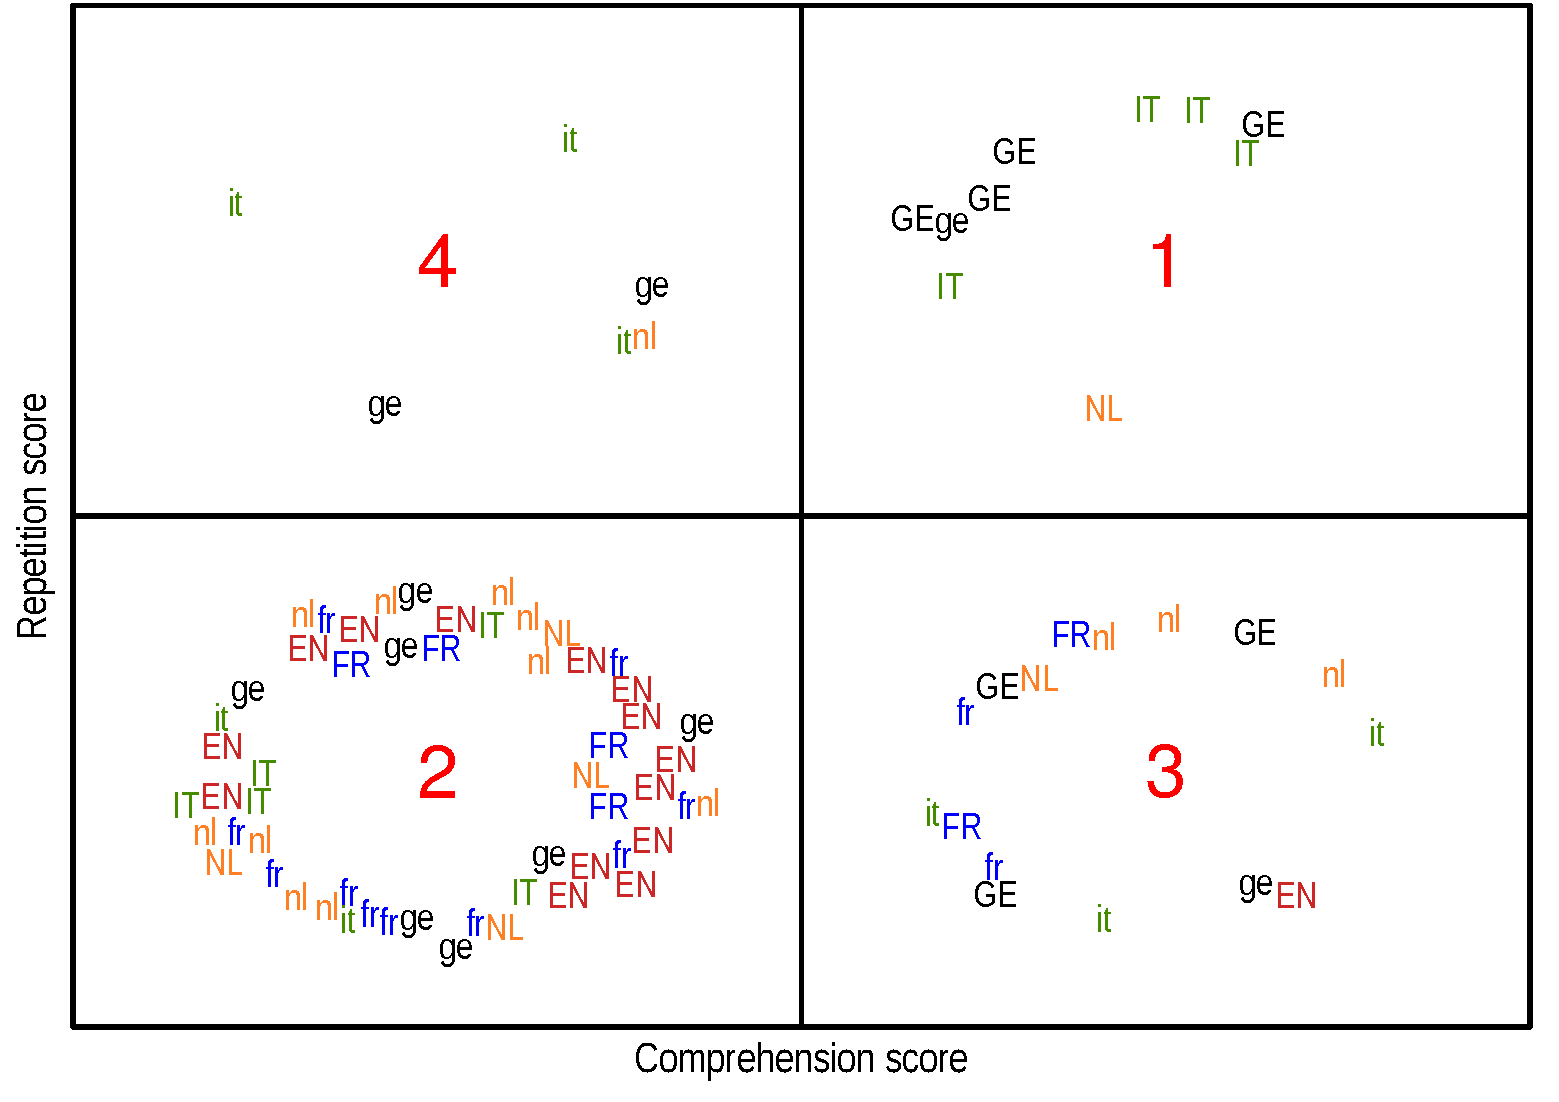
\includegraphics[width=\textwidth]{figures/06-2.pdf}
    \caption{Repetition and comprehension scores, OS targets, Time 1}
    \label{fig:06:2}
\end{figure}

An obvious cluster comprising more than a half of the dataset at T1 is located in scenario 2, indicating that neither test was performed with above chance accuracy. The second largest cluster corresponds to scenario 3, indicating above chance scores in comprehension, but not in repetition. Finally, a smaller group of learners can be found in scenario 1, indicating that already at T1 some learners managed to process OS targets morpho-syntactically in both comprehension and repetition. Coherently with the assumptions of the EI task, very few learners are found in scenario 4, which corresponds to above chance performance in repetition, but not in comprehension.

The picture presented so far is still incomplete, as it only depicts learner performance on OS targets. In order to provide a comprehensive picture of learners' processing, though, it would be desirable to have a synoptic representation of performance on SO targets as well. 

This may be exemplified by focussing on the learners located in scenario 2 in \figref{fig:06:2} (scoring at or below chance level for both comprehension and production). \figref{fig:06:3} depicts their performance on SO targets following the same rationale. 

\begin{figure}
    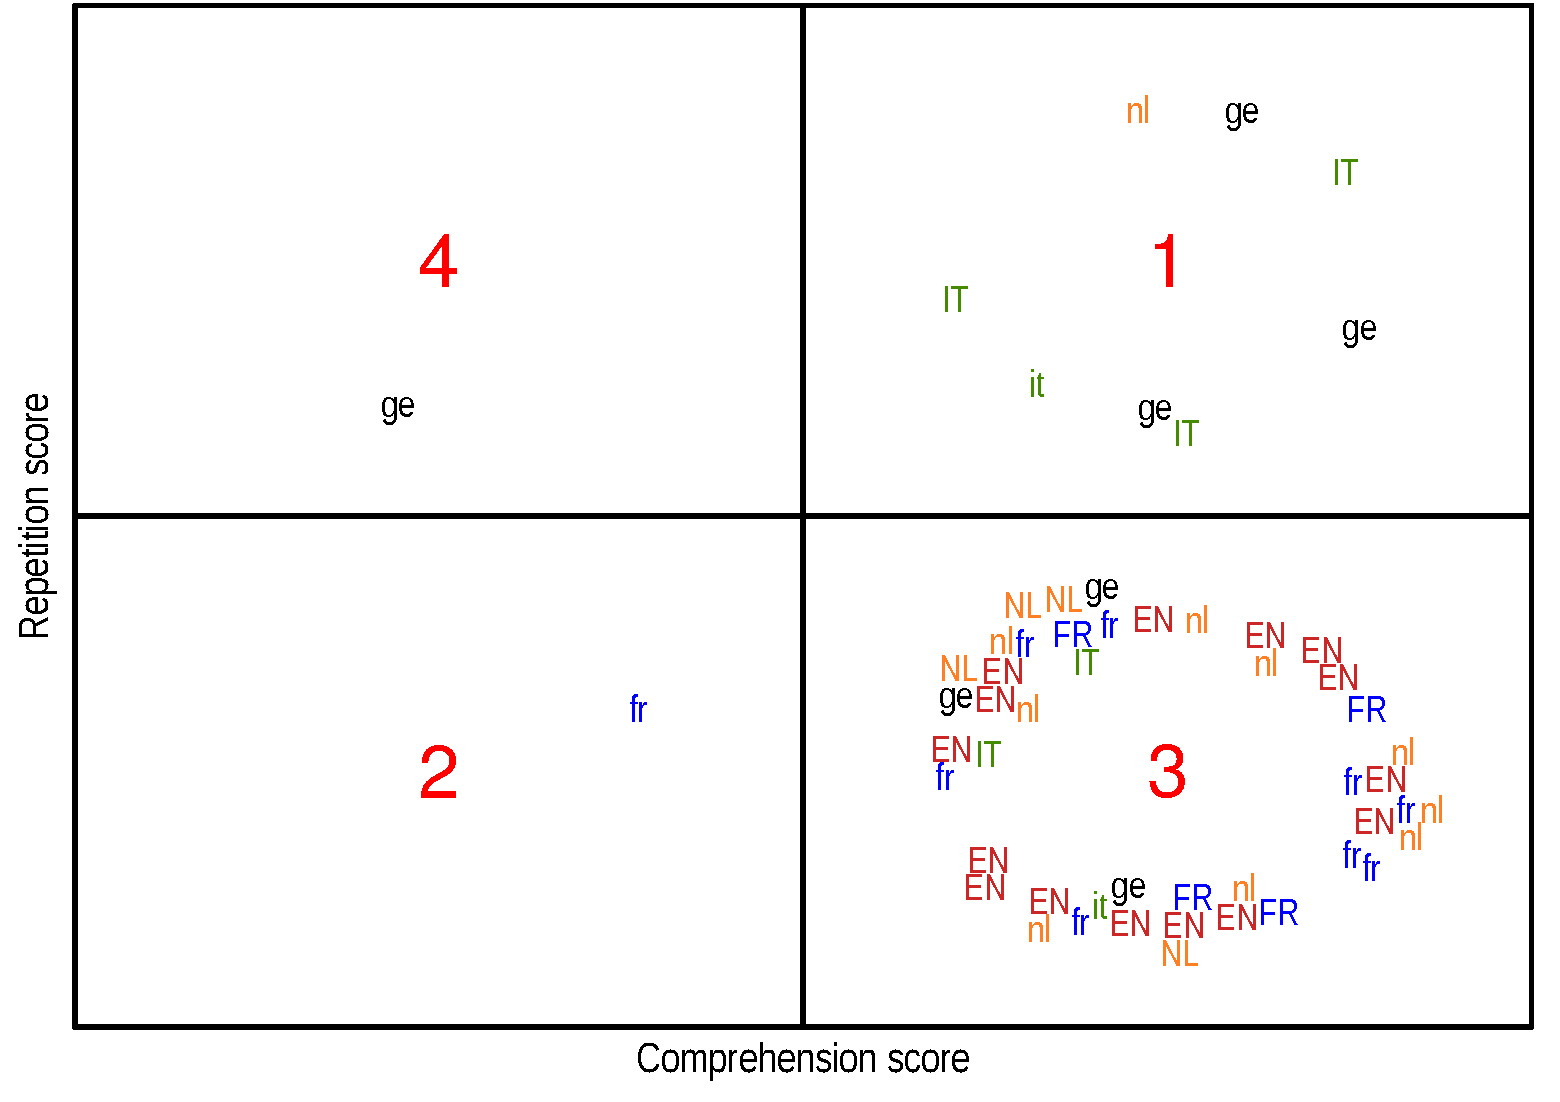
\includegraphics[width=\textwidth]{figures/06-3.pdf}
    \caption{Repetition and comprehension scores on SO targets for learners in sc. 2 on OS targets, Time 1}
    \label{fig:06:3}
\end{figure}

Again, an obvious cluster can be identified, this time in scenario 3. Such good performance on SO targets is hardly surprising, as target-like interpretation may be achieved based on either a positional or a morphosyntactic principle. The exiguity of data points in scenario 1, in contrast, witnesses to the greater difficulty of the EI task, although 8 learners do exhibit above chance accuracy. Finally, Scenarios 2 and 4 violate the assumptions of both test rationale and word order manipulation and are coherently empty.

The next step consists in merging the information presented in \figref{fig:06:2} and \figref{fig:06:3} into a single, comprehensive representation. This is achieved as shown in \figref{fig:06:4}.

\begin{figure}
    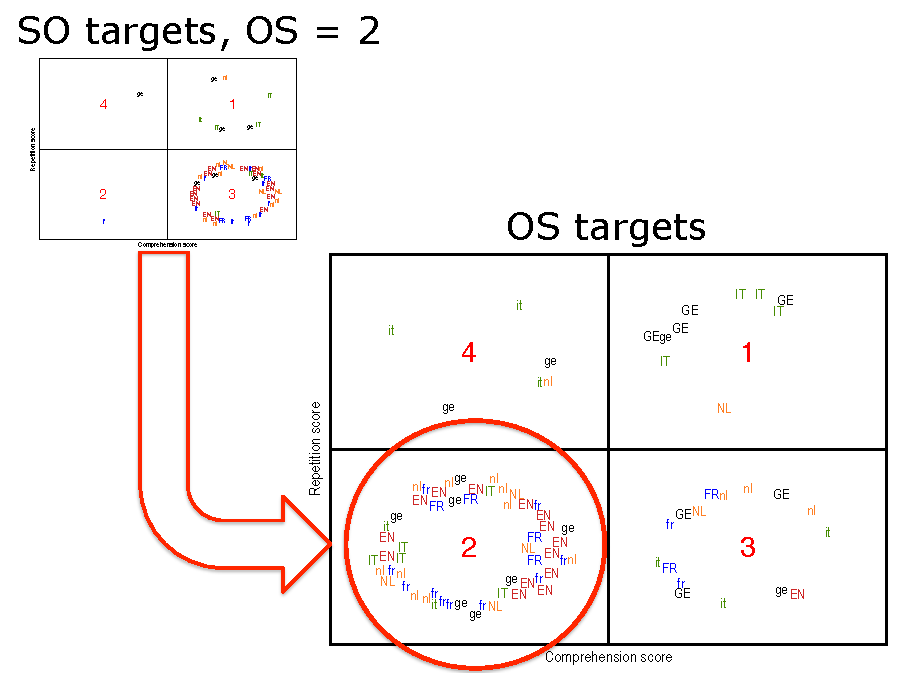
\includegraphics[width=\textwidth]{figures/06-4.pdf}
    \caption{Merging the information presented in \figref{fig:06:2} and \figref{fig:06:3}}
    \label{fig:06:4}
\end{figure}

The main squares of the graph representing the processing of OS targets are further divided into 4 minor squares, depicting the processing of SO targets by the learners comprised in the main square. Both representations rely on scenarios, arranged clockwise (4,1,3,2) for both targets, where 1 represents above-chance performance in both tests, 2 under-chance performance in both tests, and 3 and 4 depicting the situation of learners who perform above chance in one test and below in the other. To exemplify, scenario 2 on OS targets comprises 57 learners (circled in red). Based on their performance on SO targets, these learners may be grouped as follows: sc. 4: 1; sc. 1: 8; sc. 4: 1, sc. 3: 47. This distribution is graphically represented by the small square on the top left. But it would also be useful to show the performance of each learner on both SO and OS targets at the same time: to this purpose, the representation in the red circle, which only indicates sc. 2 performance on OS targets, is substituted with the square on the top left, which adds information as to the same learners’ performance on SO targets. The final result is shown in \figref{fig:06:5}.

\begin{figure}
    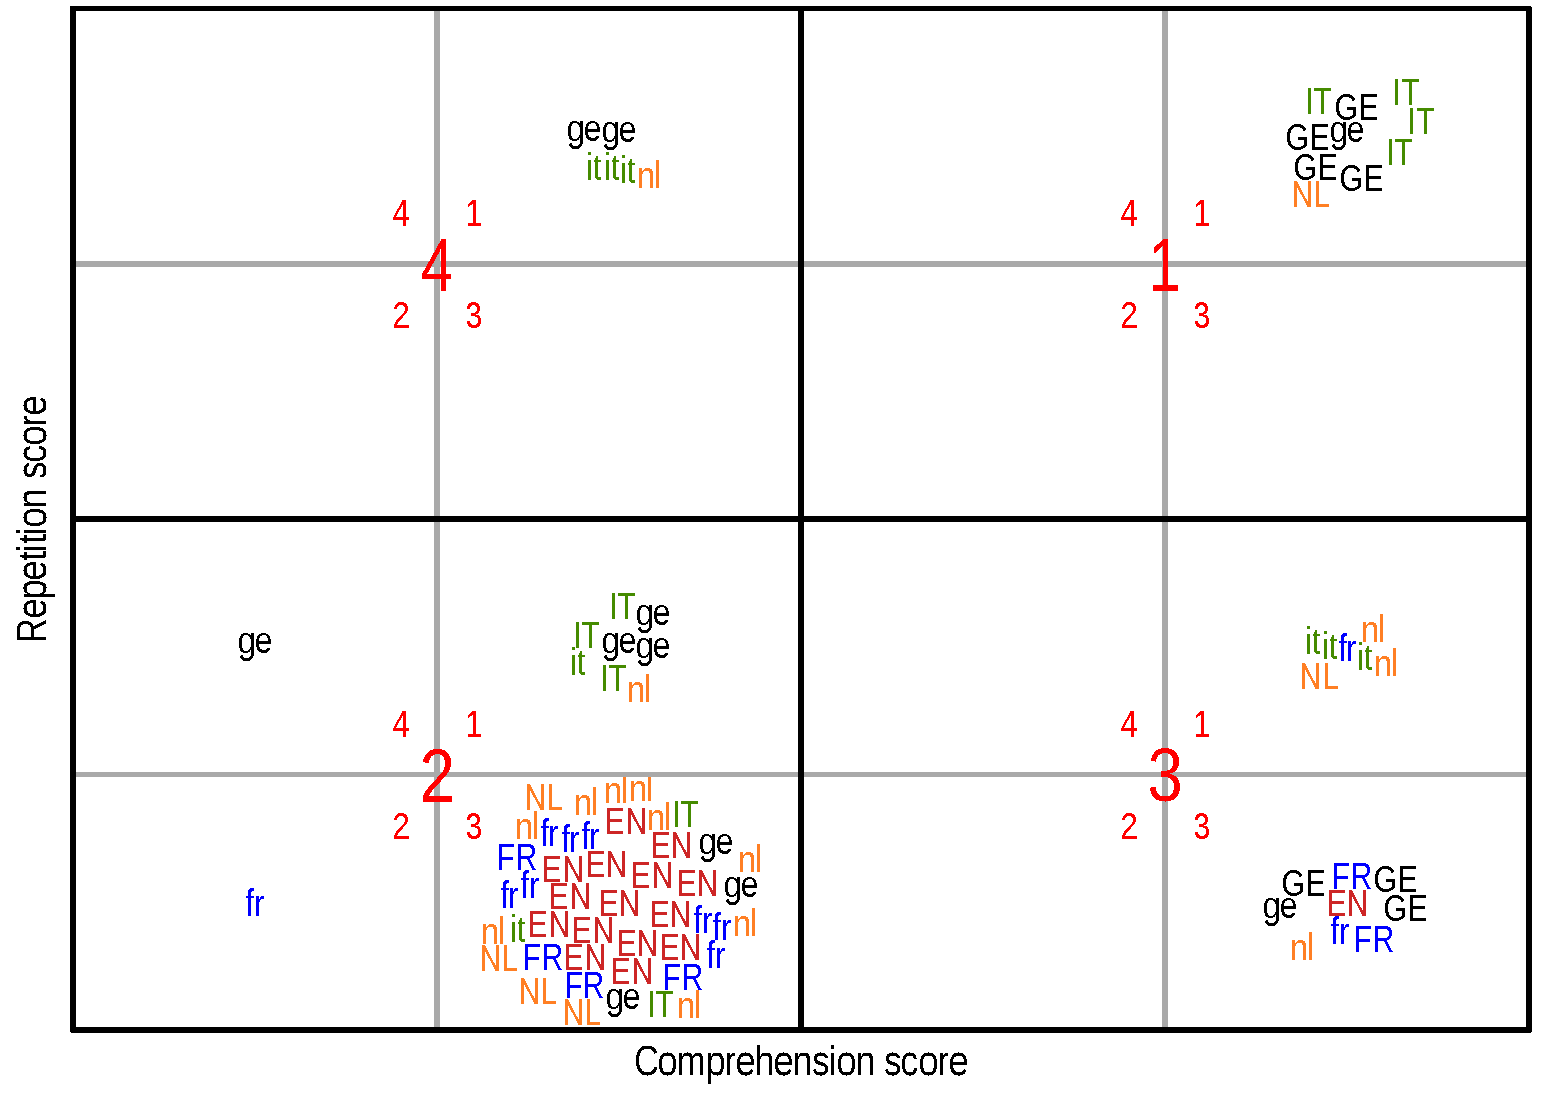
\includegraphics[width=\textwidth]{figures/06-5.pdf}
    \caption{Scenarios, T1}
    \label{fig:06:5}
\end{figure}

\section{An overall picture of learner morphosyntactic skills: results}\label{sec:06:3}

\figref{fig:06:5} is divided into 16 squares, which correspond to unique combinations of OS and SO processing scores. Each square is identified by two coordinates, corresponding to the OS scenario (large numbers) followed by the SO scenario (smaller numbers). To exemplify, scenario 2;3 corresponds to the largest cluster observed (second from left, bottom row). Again, some of the theoretically possible scenarios are linguistically unmotivated, and are accordingly empty. A rationale of linguistically motivated scenarios is provided below.

\begin{itemize}
    \item[1;1] Full morphosyntactic principle. Both tests are performed with above chance accuracy on both types of targets.
    \item [3;1] On SO targets, both tests are performed above chance; with OS targets, only the comprehension test is. The repetition of OS targets proves the hardest task.
    \item[2;1] Both tests are performed with above chance accuracy on SO targets; on OS targets, neither is. Independently of the test, OS targets are harder than SO ones.
    \item[2;3] Positional principle. only the comprehension test on SO targets is performed with above chance accuracy. 
\end{itemize}

The scenarios identified in \figref{fig:06:5} are represented analytically in \tabref{tab:06:4}. Each is broken down into its test and word order components. The last row computes the number of learners who perform above chance in each combination of test and word order. 

\begin{table}
    \begin{tabularx}{\textwidth}{XXXXXX}
    \lsptoprule
    OS repetition & OS comprehension & SO repetition & SO comprehension & scenario & n. \\
     + & + & + & + & 1;1 & 10\\
     {}- & + & + & + & 3;1 & 7\\
     {}- & {}- & + & + & 2;1 & 8\\
     {}- & {}- & {}- & + & 2;3 & 47\\
     + & {}- & + & + & 4;1 & 5\\
     {}- & + & {}- & + & 3;3 & 9\\
     {}- & {}- & + & {}- & 2;4 & 1\\
     {}- & {}- & {}- & {}- & 2;2 & 1\\
     15 & 26 & 31 & 86 &  & \\
    \lspbottomrule
    \end{tabularx}
    \caption{Implicational hierarchy at T1}
    \label{tab:06:4}
\end{table}

Following \citeauthor{AldaiWichmann2018} (\citeyear{AldaiWichmann2018}; see also \citealt{Nyqvist2018, Wichmann2015, Wichmann2016}; \citealt[210-212]{HatchLazaraton1991}), the matrix was submitted to a significance test of the degree of scalarity applying matrix randomization statistical testing (\citealt{JanssenEtAl2006}) based on Guttmann scaling. To this purpose, the R script made available by \citet{AldaiWichmann2018} as well as the \textit{vegan} R package \citep{OksanenEtAl2019} were used. A solid hierarchy emerges (GC 95,74, p < 0.01): 

OS repetition ${\supset}$ OS comprehension ${\supset}$ SO repetition ${\supset}$ SO comprehension. 

A few observations can be made. First, either task is harder on OS targets than on SO ones. Secondly, within a given constituent order, the EI task is harder than the comprehension test. Finally, all scenarios which are coherent with the hypotheses concerning constituent order and the EI task are indeed part of the hierarchy. There is an exception to this rule, however: scenario 3;3, comprising 9 learners, which is not part of the hierarchy and yet does not violate any assumption:

\begin{itemize}
    \item[3;3]  comprehension scores are above chance on both SO and OS targets, whereas repetition scores are at chance level. 
\end{itemize}

This scenario suggests that, independently of the target structure, repetition is harder for the learners than comprehension. Truly, it was not predicted that if learners can process OS targets in comprehension, they should be able to process SO targets in repetition, too. However, the vast majority appears to follow this pattern. Scenario 3;3 comprises 9 learners, whereas the closest scenario compatible with the hierarchy, namely 3;1 (success in comprehension on OS targets; success in both tests on SO targets), comprises 7 learners, so that the two situations seem equally possible. 

Another 5 learners are found in scenario 4;1, which contradicts the assumptions of the EI task: 

\begin{itemize}
    \item[4;1]  on SO targets, both tests are performed above chance; on OS targets repetition is above chance and comprehension is at chance level. 
\end{itemize}

The two remaining scenarios comprising a single learner each (2;4, 2;2) make little sense linguistically, and may be due to the participants’ lack of commitment or to random variation in their non-systematic responses. 

\subsection{Effects of additional exposure to the input}\label{sec:06:3.1}

The picture presented above describes the situation at T1 (9 hours). This section presents the results obtained after an additional 4h30 of instruction (T2). \figref{fig:06:6} presents the data in terms of scenarios.

\begin{figure}
    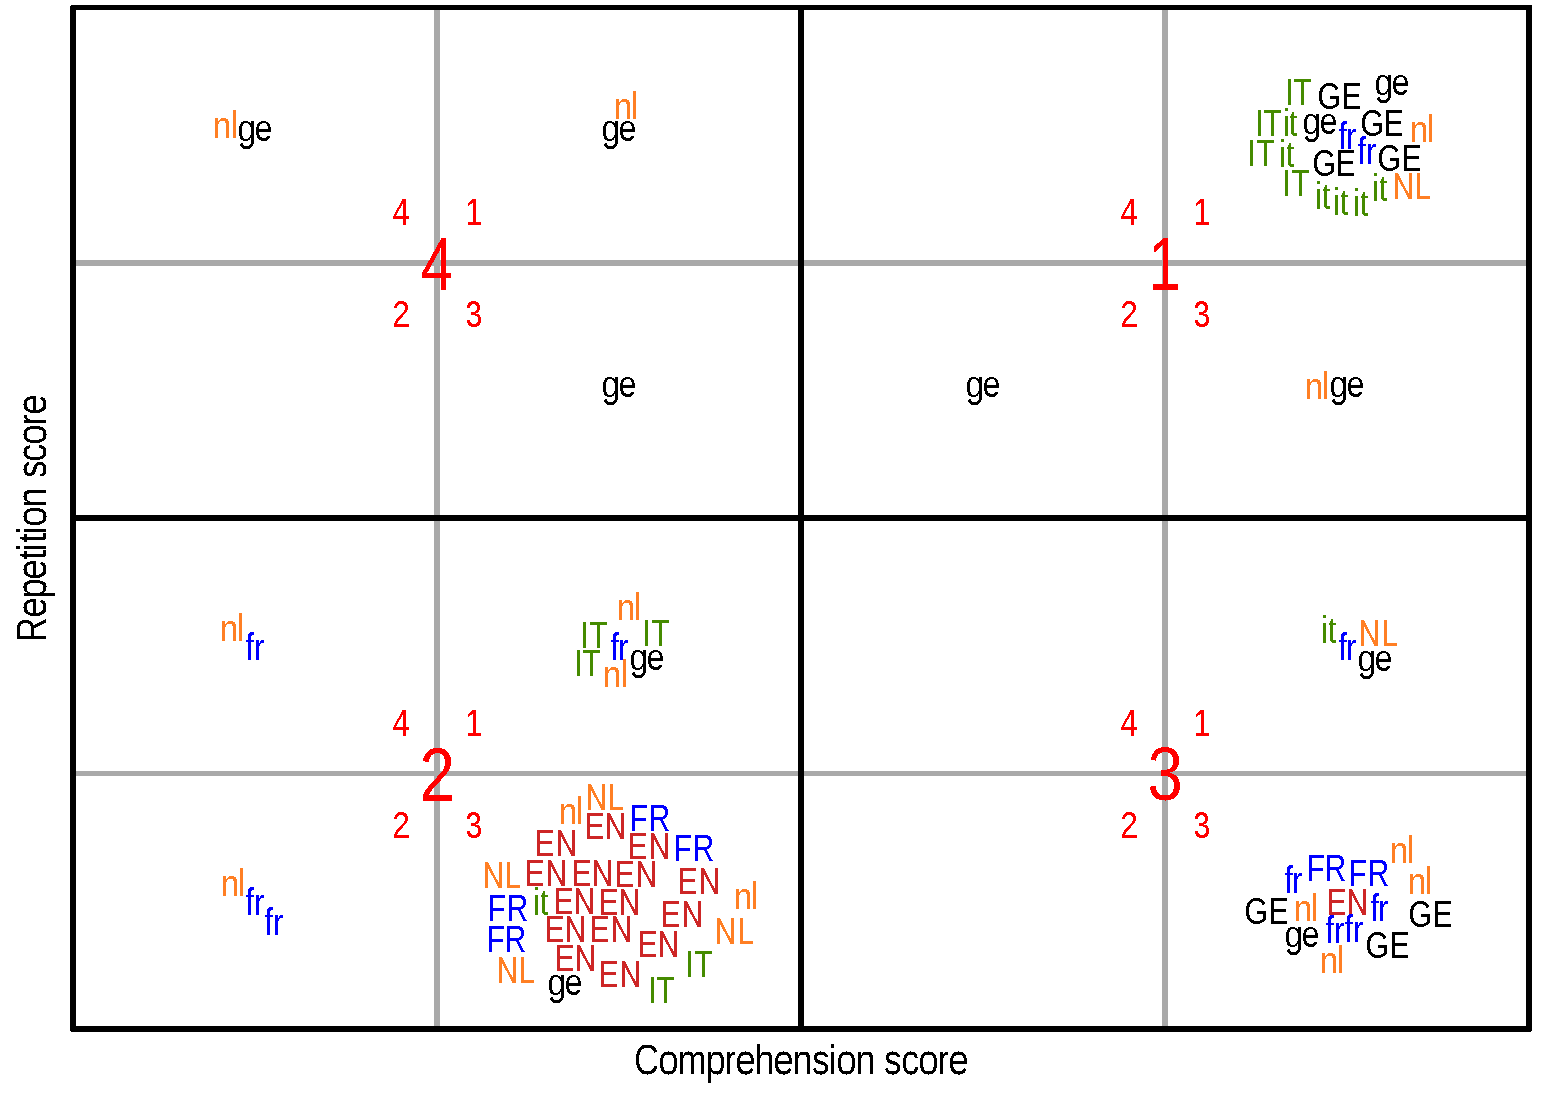
\includegraphics[width=\textwidth]{figures/06-6.pdf}
    \caption{Scenarios, T2}
    \label{fig:06:6}
\end{figure}

The main patterns observed at T1 seem to hold at T2 as well. The largest cluster still corresponds to scenario 2;3, although it now comprises fewer learners, whereas the cluster corresponding to a full morphosyntactic principle (1;1) nearly doubled. Finally, greater dispersion across scenarios is observed than at T1. The same tendencies are represented analytically in \tabref{tab:06:5}.\todo{Table 4 and 5 had both been named Table 4 and the rest had followed. Now fixed.}

\begin{table}
    \begin{tabularx}{\textwidth}{XXXXXX}
    \lsptoprule
     OS repetition & SO repetition & OS comprehension & SO comprehension & scenario & n. \\
     + & + & + & + & 1;1 & 20\\
     {}- & + & + & + & 3;1 & 4\\
     {}- & + & {}- & + & 2;1 & 7\\
     {}- & {}- & {}- & + & 2;3 & 29\\
     + & {}- & + & + & 1;3 & 2\\
     + & {}- & + & {}- & 1;2 & 1\\
     + & + & {}- & + & 4;1 & 2\\
     + & {}- & {}- & + & 4;3 & 1\\
     + & + & {}- & {}- & 4;4 & 2\\
     {}- & {}- & + & + & 3;3 & 15\\
     {}- & + & {}- & {}- & 2;4 & 2\\
     {}- & {}- & {}- & {}- & 2;2 & 3\\
     28 & 37 & 42 & 80 &  & 88\\
    \lspbottomrule
    \end{tabularx}
    \caption{Implicational hierarchy at T2}
    \label{tab:06:5}
\end{table}

Scalability analysis (GC = 92.9, p < 0,01) indicates a slightly different hierarchy than observed at T1:

OS repetition ${\supset}$ SO repetition ${\supset}$ OS comprehension ${\supset}$ SO comprehension. 

The effect of task at T2 thus appears to be slightly more relevant than that of word order, whereas the opposite was true at T1. Nevertheless, it should be pointed out that the difference between the second and the third step of the scale is minimal (5 learners at both test times).

Moving further, it is worthwhile to investigate whether any regularities may be detected in the evolution of learner processing strategies over time. Evolution patterns will be represented as a combination of the scenarios in which a learner is found at T1 and T2. 

The first column of \tabref{tab:06:6} ("pattern") lists all observed combinations of scenarios evolving from T1 to T2. This set comprises 30 items, a small fraction of the full set of possible combinations, amounting to 256 patterns, which shows that evolutionary patterns are not random

The second column shows the proportion of learners adopting each pattern. In the following columns, proportions are computed on the basis of each L1.

\begin{table}
    \begin{tabularx}{\textwidth}{XXXXXXX}
    \lsptoprule
    
    pattern & tot (n=88) & EN (n=16) & FR (n=17) & GE (n=18) & IT (n=17) & NL (n=20)\\
    2\_3 2\_3 & 28\% & 94\% & 24\% & 0\% & 12\% & 20\%\\
    1\_1 1\_1 & 10\% & 0\% & 0\% & 22\% & 24\% & 5\%\\
    2\_3 3\_3 & 8\% & 0\% & 24\% & 6\% & 0\% & 10\%\\
    3\_3 3\_3 & 7\% & 6\% & 12\% & 17\% & 0\% & 0\%\\
    3\_1 1\_1 & 5\% & 0\% & 6\% & 0\% & 18\% & 0\%\\
    2\_1 2\_1 & 3\% & 0\% & 0\% & 0\% & 18\% & 0\%\\
    2\_3 1\_1 & 3\% & 0\% & 0\% & 6\% & 6\% & 5\%\\
    2\_3 2\_1 & 3\% & 0\% & 6\% & 0\% & 0\% & 10\%\\
    2\_3 2\_2 & 3\% & 0\% & 12\% & 0\% & 0\% & 5\%\\
    2\_1 2\_3 & 2\% & 0\% & 0\% & 0\% & 6\% & 5\%\\
    2\_3 4\_4 & 2\% & 0\% & 0\% & 6\% & 0\% & 5\%\\
    3\_1 3\_3 & 2\% & 0\% & 0\% & 0\% & 0\% & 10\%\\
    4\_1 1\_1 & 2\% & 0\% & 0\% & 0\% & 12\% & 0\%\\
    1\_1 1\_2 & 1\% & 0\% & 0\% & 6\% & 0\% & 0\%\\
    2\_1 1\_1 & 1\% & 0\% & 0\% & 6\% & 0\% & 0\%\\
    2\_1 1\_3 & 1\% & 0\% & 0\% & 6\% & 0\% & 0\%\\
    2\_1 4\_1 & 1\% & 0\% & 0\% & 6\% & 0\% & 0\%\\
    2\_2 2\_4 & 1\% & 0\% & 6\% & 0\% & 0\% & 0\%\\
    2\_3 2\_4 & 1\% & 0\% & 0\% & 0\% & 0\% & 5\%\\
    2\_3 3\_1 & 1\% & 0\% & 6\% & 0\% & 0\% & 0\%\\
    2\_3 4\_1 & 1\% & 0\% & 0\% & 0\% & 0\% & 5\%\\
    2\_4 2\_3 & 1\% & 0\% & 0\% & 6\% & 0\% & 0\%\\
    3\_1 3\_1 & 1\% & 0\% & 0\% & 0\% & 0\% & 5\%\\
    3\_3 1\_1 & 1\% & 0\% & 6\% & 0\% & 0\% & 0\%\\
    3\_3 1\_3 & 1\% & 0\% & 0\% & 0\% & 0\% & 5\%\\
    3\_3 3\_1 & 1\% & 0\% & 0\% & 6\% & 0\% & 0\%\\
    4\_1 2\_1 & 1\% & 0\% & 0\% & 6\% & 0\% & 0\%\\
    4\_1 2\_3 & 1\% & 0\% & 0\% & 0\% & 0\% & 5\%\\
    4\_1 3\_1 & 1\% & 0\% & 0\% & 0\% & 6\% & 0\%\\
    4\_1 4\_3 & 1\% & 0\% & 0\% & 6\% & 0\% & 0\%\\
    \lspbottomrule
    \end{tabularx}
    \caption{Patterns of morphosyntactic processing over time}
    \label{tab:06:6}
\end{table}

The first striking observation regards the lack of clear cross-linguistic patterns in the data. Second, among the five most common patterns, three - comprising 28\%, 10\% and 7\% of the data respectively - indicate no change between T1 and T2. Next, the English L1 group is the most homogeneous - all learners but one are found in scenario 2;3, corresponding to a clear positional principle, and all learners show now change at all from T1 to T2. All other language groups exhibit more dispersion, with most clusters comprising just a single learner, and some representing a few learners. 

\section{Inferential statistics}\label{sec:06:4}

To statistically verify the tendencies identified so far, a generalised linear mixed model with binomial error structure and logit link function (Likelihood Type 3-test) was fitted to the data. The dependent variable is given by a matrix reporting each learner’s successes and failures for a given combination of predictors. Control predictors include task type (binary factor, reference level=EIT), word order (binary factor, reference level=OS), L1 (factor, EN, FR, GE, IT, NL, reference level=ENG) and test time (binary factor, reference level=T1). The interactions which proved significant in the previous analyses (i.e. L1:word order and time:word order, see sections \ref{sec:04:2.3} and \ref{sec:05:2.1}) were also added. The model is designed to test the two-way interactions concerning the predictor “task”, i.e. task:time, task:word order, task:L1, whose underlying hypothesis is that the effect of task type varies depending on target sentence word order, test time and learner L1, respectively. 

Random effects include random intercepts for participants and target items as well as correlated random slopes for time, test time and test type. 

Convergence issues unfortunately made it impossible to include a more complex structure. The summary of the model is presented in \tabref{tab:06:7}.

\begin{table}
    \begin{tabularx}{\textwidth}{lrrr}
    \lsptoprule
    \textbf{~} & \multicolumn{3}{X}{ \textbf{mat}}\\
    \textit{Predictors} & \textit{Odds} \textit{Ratios} & \textit{CI} & \textit{p}\\
    \midrule
    (Intercept) & 0.06 & 0.02~–~0.17 & \textbf{<0.001}\\
    time & 3.13 & 2.27~–~4.33 & \textbf{<0.001}\\
    L1 [FR] & 3.27 & 0.77~–~13.89 & 0.108\\
    L1 [GE] & 15.64 & 3.86~–~63.46 & \textbf{<0.001}\\
    L1 [IT] & 8.37 & 1.89~–~37.05 & \textbf{0.005}\\
    L1 [NL] & 2.52 & 0.63~–~10.20 & 0.193\\
    WO2 [SO] & 315.01 & 135.99~–~729.67 & \textbf{<0.001}\\
    test [EIT] & 0.06 & 0.02~–~0.21 & \textbf{<0.001}\\
    WO2 [SO] * test [EIT] & 0.07 & 0.04~–~0.10 & \textbf{<0.001}\\
    L1 [FR] * test [EIT] & 4.35 & 0.93~–~20.43 & 0.062\\
    L1 [GE] * test [EIT] & 18.74 & 4.12~–~85.13 & \textbf{<0.001}\\
    L1 [IT] * test [EIT] & 16.60 & 3.40~–~81.05 & \textbf{0.001}\\
    L1 [NL] * test [EIT] & 12.92 & 2.91~–~57.40 & \textbf{0.001}\\
    time * test [EIT] & 0.77 & 0.54~–~1.08 & 0.126\\
    time * WO2 [SO] & 0.46 & 0.32~–~0.64 & \textbf{<0.001}\\
    L1 [FR] * WO2 [SO] & 0.34 & 0.15~–~0.80 & \textbf{0.012}\\
    L1 [GE] * WO2 [SO] & 0.06 & 0.03~–~0.14 & \textbf{<0.001}\\
    L1 [IT] * WO2 [SO] & 1.01 & 0.40~–~2.55 & 0.979\\
    L1 [NL] * WO2 [SO] & 0.44 & 0.20~–~0.97 & \textbf{0.042}\\
    \multicolumn{4}{X}{\textbf{Random} \textbf{Effects}}\\
    σ\textsuperscript{2} & \multicolumn{3}{X}{3.29}\\
    τ\textsubscript{00}~\textsubscript{participant} & \multicolumn{3}{X}{3.30}\\
    τ\textsubscript{00}~\textsubscript{participant.1} & \multicolumn{3}{X}{1.00}\\
    τ\textsubscript{00}~\textsubscript{participant.2} & \multicolumn{3}{X}{2.19}\\
    τ\textsubscript{11}~\textsubscript{participant.testEIT} & \multicolumn{3}{X}{4.03}\\
    τ\textsubscript{11}~\textsubscript{participant.1.WO2SO} & \multicolumn{3}{X}{0.52}\\
    τ\textsubscript{11}~\textsubscript{participant.2.time} & \multicolumn{3}{X}{1.30}\\
    ρ\textsubscript{01}~\textsubscript{participant} & \multicolumn{3}{X}{{}-0.82}\\
    ρ\textsubscript{01}~\textsubscript{participant.1} & \multicolumn{3}{X}{{}-1.00}\\
    ρ\textsubscript{01}~\textsubscript{participant.2} & \multicolumn{3}{X}{{}-1.00}\\
    ICC & \multicolumn{3}{X}{0.41}\\
    N~\textsubscript{participant} & \multicolumn{3}{X}{91}\\
    Observations & \multicolumn{3}{X}{720}\\
    Marginal R\textsuperscript{2}~/ Conditional R\textsuperscript{2} & \multicolumn{3}{X}{0.494 / 0.704}\\
    \lspbottomrule
    \end{tabularx}
    \caption{Model output}
    \label{tab:06:7}
\end{table}

The interactions involving the predictor “test” were tested by comparing the full model described above to three reduced models, each lacking the single interaction of interest (\tabref{tab:06:8}).

\begin{table}
    \begin{tabularx}{\textwidth}{XXXX}
    \lsptoprule
    predictor & Chisq & Df & Pr(>Chisq)\\
    task : word order & 191.892 & 1 & < 0.01\\
    task : L1 & 17.557 & 4 & < 0.01\\
    task : time & 2.339 & 1 & > 0.05\\
    \lspbottomrule
    \end{tabularx}
    \caption{Single-term deletion}
    \label{tab:06:8}
\end{table}

Pairwise comparisons show that the predictors interact in a complex way, producing numerous statistically significant contrasts. Performance in the two tasks was usually statistically significant, which confirms the initial hypothesis that the EIT is indeed more demanding than the comprehension task. The only contrasts which proved \textit{not} significant involved the OS word order and the German, Italian and Dutch L1 groups at both test times.

\subsection{Repetition in the absence of comprehension}\label{sec:06:4.1}

The rationale of the analysis presented so far is that learner comprehension and repetition scores combined should provide a comprehensive picture of the principles of utterance organisation observable in the learner variety. The validity of this approach relies on the assumptions of the EI task, namely that target repetition is impossible without its comprehension. Phonological memory should not play any significant role in this test. 

Nevertheless, a few learners appear to violate this assumption. For each relevant combination of test time and word order, \tabref{tab:06:9} provides comprehension and repetition scores of learners who at least at one test time appeared in scenario 4, along with the probability of observing such a distribution in the absence of a rational morpho-syntactic principle. Information as to the learners' performance in terms of scenarios at T1 and T2 is also provided in the last two columns. The table shows that repetition and comprehension scores are consistently very high or very low, which excludes the possibility that the subject were assigned to scenario 4 only because they slightly exceeded score thresholds. 

\begin{table}
    \begin{tabularx}{\textwidth}{XXXXXXXXXXX} & time & WO & subj. & L1 & rep. score & rep. p & comp. score & comp. p & sc. T1 & sc. T2\\
    \lsptoprule
    a. & 1 & OS & 2108 & NL & 0.88 & < 0.01 & 0.00 & 1.00 & 4\_1 & 2\_3\\
    b. & 1 & OS & 4105 & GE & 0.80 & 0.03 & 0.44 & 0.60 & 4\_1 & 4\_3\\
    c. & 1 & OS & 4108 & GE & 0.83 & 0.02 & 0.31 & 0.89 & 4\_1 & 2\_1\\
    d. & 1 & OS & 5104 & IT & 0.71 & 0.06 & 0.38 & 0.77 & 4\_1 & 1\_1\\
    e. & 1 & OS & 5106 & IT & 0.75 & 0.04 & 0.00 & 1.00 & 4\_1 & 3\_1\\
    f. & 1 & OS & 5109 & IT & 0.86 & 0.01 & 0.00 & 1.00 & 4\_1 & 1\_1\\
    g. & 2 & OS & 2118 & NL & 0.88 & < 0.01 & 0.00 & 1.00 & 2\_3 & 4\_1\\
    h. & 2 & OS & 4105 & GE & 1.00 & < 0.01 & 0.31 & 0.89 & 4\_1 & 4\_3\\
    i. & 2 & OS & 4110 & GE & 1.00 & < 0.01 & 0.31 & 0.89 & 2\_1 & 4\_1\\
    l. & 1 & SO & 4112 & GE & 1.00 & < 0.01 & 0.50 & 0.36 & 2\_4 & 2\_3\\
    m. & 2 & SO & 1119 & FR & 0.75 & 0.04 & 0.12 & 0.96 & 2\_2 & 2\_4\\
    n. & 2 & SO & 2115 & NL & 0.88 & < 0.01 & 0.14 & 0.94 & 2\_3 & 2\_4\\
    \lspbottomrule
    \end{tabularx}
    \caption{Learners in scenario 4}
    \label{tab:06:9}
\end{table}

Participants in scenarios 2;4 and 4;4 exhibit higher scores in repetition than comprehension. This behaviour is hardly explicable in that they fail to score above chance in the comprehension of SO targets, which can be indifferently processed based on word order or inflectional morphology. A single participant is located in scenario 4;3, which surprisingly indicates above chance repetition of OS, but not SO targets, and just the opposite situation in the comprehension test. Such behaviour seems rather erratic and does not lend itself to a specific explanation. It must be mentioned, nevertheless, that results may slightly inflated because of repeated statistical testing. 

The facts reported above should induce a little caution as to the assumptions of the EI task. This section therefore aims to verify whether or not it is really possible to perform the EI task in the absence of comprehension. To this end, the VILLA EI task was administered to new groups of Italian, French and German participants selected on the basis of the VILLA guidelines (see section \ref{sec:06:2.3}\todo{No such section!})\footnote{Italian participants were recruited by the authour with the help of prof. Bernini and tested at the University of Bergamo; French and German participants were recruited and tested by Marzena Wątorek at the CNRS SFL, Paris, and by Christine Dimroth and Johanna Hinz at Münster University, respectively. Sincere thank to all of them for their helpful effort.}. These new test-takers were not exposed to any Polish input, so that it was impossible for them to process target sentences for meaning: the only skills they brought to the task was their phonological memory. Their performance therefore should be comparable to that of a VILLA subject who did not process targets for meaning, but only repeated them as a string of sounds. Will these participants with no comprehension skills be able to repeat ACC case endings? If that were the case, we should conclude that the VILLA EI task does not fulfil the assumptions of this kind of task.

A few examples of repetitions of the target sentence in \REF{ex:06:4a} are presented in (\ref{ex:06:4b}-d).

\ea%4
    \label{ex:06:4}
    \ea\label{ex:06:4a}
    \gll    /ʥevˈʧɨnk-e  ˈʨɔngnje  portuˈgalk-a/ \\
            little.girl-\textsc{acc}   pulls     Portuguese.woman-\textsc{nom}\\
    \ex\label{ex:06:4b}
    [ˈʧefnie ne'tswo na portuˈgala] \hfill (German group, subject 2)
    \ex\label{ex:06:4c}
    [dʒiˈkinʧi ˈkɔnʧe portuˈgarʧe] \hfill (French group, subject 1)
    \ex\label{ex:06:4d}
    [tsipˈtirne ʧo portuˈgal kta] \hfill (Italian team, subject 3)
    \z
\z

The two non-transparent words /ʥevʧɨnke/ and /ʨɔngnje/ are hardly recognisable, whereas the transparent word in final position sounds decidedly closer to the target, although accurate repetitions only concern that part of the word which is recognisable in both the target language and the subject's L1, namely the stem /portugal/. Suffixes and inflectional endings are mostly omitted or substituted with random linguistic material. At the same time, in some cases the segments corresponding to case endings are correctly repeated, in spite of being attached to a more or less random sequence of sounds, as [e] in [tsiptirne] \REF{ex:06:4d}. Since processing for meaning is to be excluded, one has to admit that the repetition of those segments can only be due to phonological memory. This too, however, is by no means a rule: working memory also seems prone to errors and inaccuracies, as witnessed by [e] in [portugarʧe] in \REF{ex:06:4c} for target [a] in /portuˈgalka/.

Nevertheless, comparing the output of the VILLA learners to that of first-exposure participants is not necessarily a legitimate operation. The examples in (\ref{ex:06:5b}-m\todo{n updated as m. There was no item j in the manually created list.}) report the repetition of the target sentence in \REF{ex:06:5a} as performed by learners who perform above chance in repetition, but not comprehension. Leaving inflectional endings aside for the moment, the output produced by these learners is quite different from that of the informants in \REF{ex:06:4}, as lexical items are clearly recognisable and produced with considerable accuracy. The overall picture will be discussed and interpreted in the following chapter on semi-spontaneous production (7)\todo{Add chapter link}.

\ea%5
    \label{ex:06:5}
    \ea\label{ex:06:5a}
    \gll    /ʥevˈʧɨnk-e   ˈʨɔngnje   portuˈgalk-a/\\
            little.girl-\textsc{acc}   pulls     Portuguese.woman-\textsc{nom}\\
    \ex\label{ex:06:5b}
    [dʒewˈʧɨnke ˈʧɔngnie portuˈgalka]
    \ex\label{ex:06:5c}
    [dʒewˈʧenkə portuˈgalska]
    \ex\label{ex:06:5d}
    [dʒewˈʧɨnknɛ ˈportu ˈporta ˈbazu port portuˈgalka]
    \ex\label{ex:06:5e}
    [dʒjefˈʧɨnka dʒ ˈʧɔɲɲe portuˈgalka]
    \ex\label{ex:06:5f}
    [dʒjefˈʧɨnka kn eh ˈʧɔɲe portuˈgalkon]
    \ex\label{ex:06:5g}
    [portuˈgalka]
    \ex\label{ex:06:5h}
    [dʒewˈʧinke ˈʧɔngnie portuˈgalka]
    \ex\label{ex:06:5i}
    [dʒewˈʧɨnə ˈʧorgo portuˈgalka]
    \ex\label{ex:06:5j}
    [dsziewˈʧɨnkɛ ˈʧgnie portuˈgalka]
    \ex\label{ex:06:5k}
    BLANK
    \ex\label{ex:06:5l}
    [portuˈgalka ˈʧɔɲe dʒefˈkinkje]
    \ex\label{ex:06:5m}
    [portuˈgalke ˈʧɔngnie dʒewˈʧɨnke]
    \z
\z

\section{Conclusion}\label{sec:06:5}

Clear tendencies emerge from the analysis of morphosyntactic skills in the structured tests, pointing to the relatively greater difficulty of the EI task and of OS targets. Even though the majority of learners consistently apply a positional principle of utterance organisation, it is an impressive result that at least a fraction of them seems to be able to apply a morphosyntactic principle after only 9 hours. Their number increases with additional, albeit limited input exposure, suggesting that even complex target structures may be acquired spontaneously with no explicit instruction and within only hours from the first contact with the target language.

\chapter{Semi-spontaneous production}\label{sec:6}

\section{Research questions and rationale}\label{sec:07:1}

Following the analysis of learner performance in the structured tests, the present chapter aims to observe learner morphosyntactic skills in a more realistic communicative situation, arguably closer to real language use. To this end, it presents and discusses the output elicited through a semi-spontaneous production task in which learners took part in pairs or small groups. Because of the amount of work required to transcribe and analyse such interactional data, only a subset of the database (the Italian Meaning Based edition of the project) will be considered.

After a qualitative analysis of learner-produced utterances, the study will apply the same statistical tool employed in the previous chapters in order to determine whether or not learners may thought to apply a morphosyntactic principle in their output. The results are then compared to the scenarios identified in the previous chapters in order to appropriately collocate semi-spontaneous production along an implicational scale of task difficulty.

\section{An overview of learner output}\label{sec:07:2}

In learner’s utterances, new referents are typically introduced by a copular construction with presentative function, in which the topic is expressed by a personal pronoun (\textit{on,} ‘he’ or \textit{ona}, ‘she’) and the complement is instantiated by the name of the character \REF{ex:07:1}.

\ea%1
    \label{ex:07:1}
    \ea\label{ex:07:1a}
    \gll    [ɔna   jɛst   ʤovann-a].\\
            \hspaceThis{[}she  is  Giovanna-\textsc{nom}\\
    \glt    ‘She is Giovanna.’
    \ex\label{ex:07:1b}
    \gll    [ʤovann-a     ɛst   nauʧiʧɛlk-on].  \\
            \hspaceThis{[}Giovanna-\textsc{nom}  is  teacher-\textsc{ins}\\
    \glt    ‘Giovanna is a teacher.’
    \z
\z

When a referent has been introduced, it is typically referred to using personal pronouns \REF{ex:07:2}, although person names may be repeated in consecutive utterances \REF{ex:07:3}:

\ea%2
    \label{ex:07:2}
    \ea\label{ex:07:2a}
    \gll    [to   jest   marj-a].\\
            \hspaceThis{[}this  is  Maria-\textsc{nom}\\
    \glt    ‘This is Maria.’
    \ex\label{ex:07:2b}
    \gll    [ɔna   lubi   herbat-a].\\
            \hspaceThis{[}she  likes  tea-\textsc{nom}\\
    \glt    ‘She likes tea.’
    \z
\z

\ea%3
    \label{ex:07:3}
    \ea\label{ex:07:3a}
    \gll    [to   jest   marj-a].\\
            \hspaceThis{[}this  is  Maria-\textsc{nom}\\
    \glt    ‘this is Maria’
    \ex\label{ex:07:3b}
    \gll    [marj-a   jest   njemk-on  i   tumaʧk-on].\\
            \hspaceThis{[}Maria-\textsc{nom}  is  German-\textsc{ins}  and  interpreter-\textsc{ins}\\
    \glt    ‘Maria is German and an interpreter.’
    \z
\z

Zero anaphora can be encountered \REF{ex:07:4b} following utterances in which the subject is expressed by either a name or a pronoun \REF{ex:07:4a}.

\ea%4
    \label{ex:07:4}
    \ea\label{ex:07:4a}
    \gll    [ɔna     jɛst   portugalk-on (...)].\\
            \hspaceThis{[}she\textsc{.nom}  is  Portuguese-\textsc{ins}\\
    \glt    ‘She is Portuguese.’
    \ex\label{ex:07:4b}
    \gll    [i   zna   jɛski         angjelsk-i].\\
            \hspaceThis{[}and  knows  language\textsc{.nom/acc(?)}  English-\textsc{nom}/\textsc{acc} \\
    \glt    ‘And she speaks English.’
    \z
\z

No examples can be found in which common nouns express the subject function. 

Nouns in the object function may be correctly marked as accusative, both in a sequence of feminine nouns only \REF{ex:07:5a} and in sequences containing both feminine and masculine nouns  (\ref{ex:07:5b}, where \textit{kot} ‘cat’ and \textit{pies} ‘dog’ are masculine):

\ea%5
    \label{ex:07:5}
    \ea{\label{ex:07:5a}
    \gll    [ɔn   lubi   ʧokolad-e     kav-e     i   erbat-e].\\
            \hspaceThis{[}He  likes  chocolate-\textsc{acc}    coffee-\textsc{acc}  and  tea-\textsc{acc}\\}\jambox*{(5106)}
    \glt    ‘He likes chocolate, coffee and tea.’
    \ex{\label{ex:07:5b}
    \gll    [kɔxa  ʒɔn-e    ev-e    kɔt-a    i  ps-a].\\
            \hspaceThis{[}loves  wife-\textsc{acc}  Ewa-\textsc{acc}   cat-\textsc{acc}    and  dog-\textsc{acc}\\}\jambox*{(5111)}
    \glt    ‘(he) loves his wife Ewa and (his) cat and (his) dog’
    \z
\z

At the other end of the spectrum, occurrences can be found in which all feminine nouns in the object function are marked as nominative \REF{ex:07:6}:

\ea%6
    \label{ex:07:6}
    \ea{\label{ex:07:6a}
    \gll    [ɔna   lubi   herbat-a].\\
            \hspaceThis{[}she  likes  tea-\textsc{nom}\\}\jambox*{(5119)}
    \glt    ‘She likes tea.’
    \ex{\label{ex:07:6b}
    \gll    [ɔna   lubi   ʧekolad-a     kav-a     i   erbat-a].\\
            \hspaceThis{[}she  likes  chocolate-\textsc{nom}  coffee-\textsc{nom}  and  tea-\textsc{nom}\\}\jambox*{(5107)}
    \glt    ‘She likes chocolate coffee and tea.’
    \z
\z

In other cases still, feminine nouns with the object function seem to randomly appear with a nominative or accusative endings, with no apparent regularity \REF{ex:07:7}:

\ea{%7
    \label{ex:07:7}
    \gll    {ɔna}   {lubi}   {erbat-e}   {i}   {kav-a.}\\
            she  likes  tea-\textsc{acc}  and  coffee-\textsc{nom}\\}\jambox*{(5107)}
    \glt    ‘She likes tea and coffee.’
    \z

Errors in the case marking of the object most commonly involve an overextension of the NOM ending [a]. Marginal non-target-like endings include bare consonants and [ən], with 6 and 1 instances respectively (\tabref{tab:07:1}). In some cases the influence of other known languages can be hypothesised, as in [matema'tik] as opposed to German \textit{Mathematik} /matemaˈtiːk/. In other cases, the ending may be modelled on other word forms present in the input: in [kerbatən], for instance, the ending [ən] may be a trace of the instrumental masculine ending -\textit{em} [em]. 

\begin{table}
    \begin{tabularx}{\textwidth}{llll}
        \lsptoprule
        learner & utterance & learner form & target\\
        5101 & [i ma dzurk]. & [dzurk] & /tsurke/\\
        5118 & [paolo lubi matema'tik i mu'zik]. & [matema'tik] & /mate'matɨke/\\
        5118 & [paolo lubi matema'tik i mu'zik]. & [mu'zik] & /'muzɨke/\\
        5115 & [on lubi literatura i matematik]. & [matematik] & /mate'matɨke/\\
        5117 & [ɔn lubi matematik i psa]. & [matematik] & /mate'matɨke/\\
        5117 & [marta lubi kav i kerbatən]. & [kav] & /'kave/\\
        5117 & [marta lubi kav i kerbatən]. & [kerbatən] & /her'bate/\\
        \lspbottomrule
    \end{tabularx}
    \caption{Semi-spontaneous production task, endings other than -/a/ or -/e/}
    \label{tab:07:1}
\end{table}

As such non-target endings were produced by only four learners, it seems that this phenomenon should be a matter of individual variability whose causes are beyond experimental control. 

No examples of OS word order were found in the data. 

\subsection{Morphological variability and relation to the input}\label{sec:07:2.1}

The present section aims to describe morphological variability among the lexemes which occur in the OBJ function. The purpose of this step is to verify whether or not the semantics of specific lexical items associates them more closely to either syntactic function (as indeed is the case in the input, see chapter 3) and consequently to a specific inflectional ending. 

To this purpose, \tabref{tab:07:2} lists the lexemes produced by learners along with their English translation. For each entry, the table indicates first the citation form and its English translation, then the overall accuracy with which the word received accusative marking ("mean"). This value is computed as the ratio between the number of accusative forms and the total number of occurrences ("freq") produced by all participants in contexts expressing the Object function. The following column (“participants”) indicates the number of participants who produced the lexeme (regardless of how it was inflected). The last four columns provide the frequency with which the word occurred in the input at the time of the test, i.e. after 10:30 hours. Figures are presented relatively to the NOM and ACC cases as well as and cumulatively for all other cases combined ("other"). Given the nature of the task, not many occurrences were elicited for each lexeme: the most common item (\textit{literatura}, ‘literature’) occurred 17 times in the whole data-set, while 6 words (e.g. \textit{rodzina}, ‘family’) only occurred once. 

\begin{table}
    \fittable{
    \begin{tabular}{ll r rrrrrr}
         &  & \multicolumn{3}{c}{ output} & \multicolumn{4}{c}{ input}\\
        \lsptoprule
        lexeme & translation & Mean & Freq. & participants & NOM & ACC & other & Tot\\
        \midrule
        \textit{Chorwacja} & Croatia & 1.00 & 2 & 1 & 1 & 0 & 2 & 3\\
        \textit{Ewa} & Ewa & 1.00 & 2 & 1 & 123 & 4 & 34 & 161\\
        \textit{rodzina} & family & 1.00 & 1 & 1 & 32 & 0 & 12 & 44\\
        \textit{tata} & dad & 1.00 & 1 & 1 & 54 & 19 & 0 & 73\\
        \textit{żona} & wife & 1.00 & 2 & 1 & 44 & 4 & 0 & 48\\
        \textit{herbata} & tea & 0.78 & 9 & 9 & 16 & 52 & 0 & 68\\
        \textit{kuchnia} & cuisine/kitchen & 0.75 & 4 & 3 & 20 & 22 & 0 & 42\\
        \textit{literatura} & literature & 0.71 & 17 & 11 & 1 & 53 & 0 & 54\\
        \textit{matematyka} & math & 0.57 & 7 & 5 & 0 & 9 & 0 & 9\\
        \textit{kola} & coke & 0.50 & 2 & 2 & 8 & 30 & 0 & 38\\
        \textit{mama} & mum & 0.50 & 2 & 1 & 54 & 8 & 0 & 62\\
        \textit{żaba} & frog & 0.50 & 2 & 2 & 61 & 48 & 0 & 109\\
        \textit{piłka} & ball & 0.33 & 3 & 3 & 30 & 23 & 0 & 53\\
        \textit{czekolada} & chocolate & 0.30 & 10 & 6 & 13 & 58 & 0 & 71\\
        \textit{kawa} & coffee & 0.30 & 10 & 6 & 36 & 48 & 0 & 84\\
        \textit{Anna} & Anna & 0.00 & 1 & 1 & 243 & 0 & 2 & 245\\
        \textit{córka} & daughter & 0.00 & 6 & 5 & 27 & 4 & 0 & 31\\
        \textit{lalka} & doll & 0.00 & 1 & 1 & 22 & 7 & 9 & 48\\
        \textit{muzyka} & music & 0.00 & 1 & 1 & 1 & 19 & 0 & 20\\
        \textit{pizza} & pizza & 0.00 & 1 & 1 & 12 & 31 & 0 & 43\\
        \textit{siostra} & daughter & 0.00 & 3 & 2 & 19 & 13 & 3 & 45\\
        \lspbottomrule
    \end{tabular}
    }
    \caption{Lexemes produced by learners in interaction}
    \label{tab:07:2}
\end{table}

The following analysis is limited to common nouns, which leads to the exclusion of the names \textit{Anna,} \textit{Ewa} and \textit{Chorwacja}, ‘Croatia’. The rationale for this decision is that proper names may not be treated as common nouns, despite the fact that, in Polish, they are inflected  along the same inflectional paradigm. 

A certain degree of variability can also be found in the overall input frequency of the items considered here, the two extremes of the continuum being \textit{matematyka}, ‘mathematics’, with just 9 occurrences, and \textit{żaba}, ‘frog’, with 109. 

Regarding morphosyntactic accuracy, the whole continuum from 100\% to 0\% is represented. As made clear by example \REF{ex:07:7} above, different nouns may receive either marking even within the same utterance. 

It may be hypothesised that this variability in morpho-syntactic accuracy may result from a biased distribution in the input: if a given lexeme mostly occurs in a specific word-form, then learners may associate it with the corresponding syntactic function or, at least, with the corresponding case marking. To exemplify, if a word only occurs in the accusative case, like \textit{matematyka,} ‘mathematics’, learners may note and remember it in its accusative form only. If this is the case, then accuracy for accusative case marking should be very high, in principle 100\%. In addition, this word-form should overextend to all others, including the nominative case: in other words, the basic word-form of this lexical item should be modelled on the accusative case.

One way to explain the observed variability in the accuracy of ACC marking is to hypothesise that this might be influenced by the proportion of instances in which a given lexeme appears in that word-form in the input. The more commonly the word appears in the input as ACC as opposed to NOM, the more accurately it should be marked as ACC in learner output as well.

If this is the case, plotting the relative frequency of accusative forms against case-marking accuracy should result in a straight line with a positive slope. \figref{fig:07:7}.1, however, shows no apparent pattern, suggesting that the expectations are not borne out in the data. A few words which in the input hardly ever occur in the accusative case show a mean accuracy of 100\% (e.g. \textit{rodzina} ‘family’), while others, whose ACC word form is much more common, exhibit much lower accuracy scores (e.g. \textit{muzyka} ‘music’).

\begin{figure}
    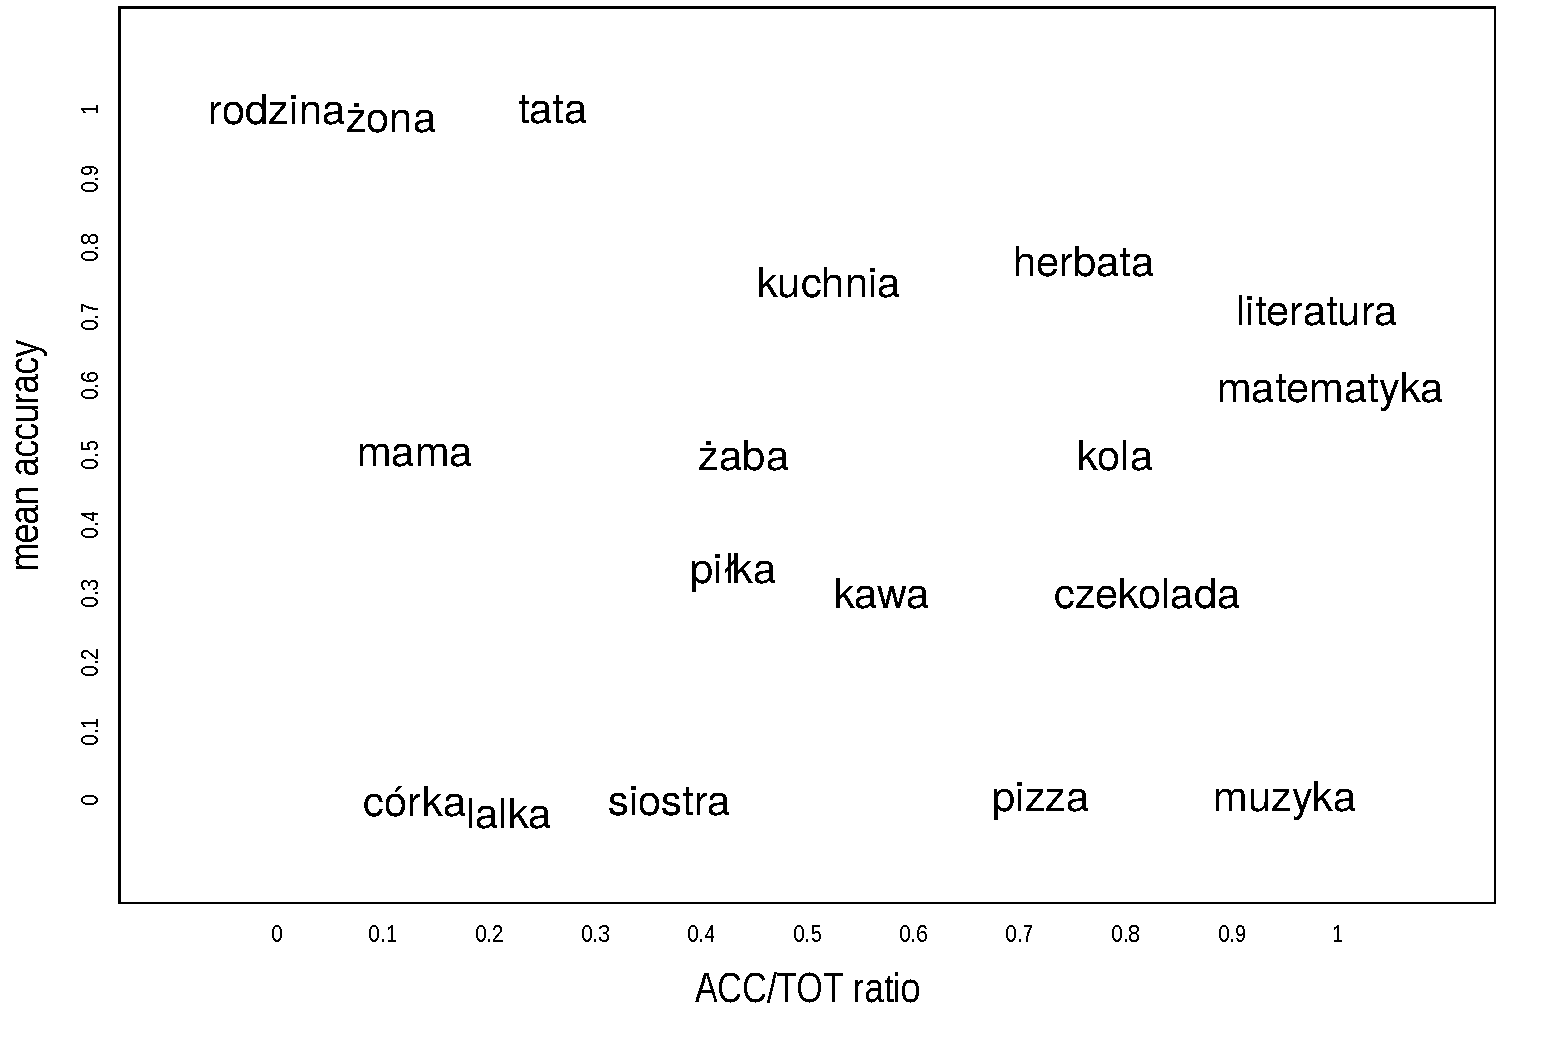
\includegraphics[width=\textwidth]{figures/07-1.pdf}
    \caption{Semi-spontaneous production, mean accuracy and ACC/TOT ratio}
    \label{fig:07:1}
\end{figure}

One may now consider the cumulative frequency of a given lexical item, in order to verify the claim that if a word is very frequent in the input, then it should be more available to the learners, and therefore more easily retrievable. In turn, if a word is easily retrievable, then perhaps the learner could devote more resources to inflectional morphology. 

If there were a correlation between overall lexical frequency and grammatical accuracy, lexemes in \figref{fig:07:2} should distribute along a positive slope, with accuracy increasing together with input frequency. Quite clearly, this is not the case. Differences in learner morphosyntactic skills thus do not seem due to a biased distribution of word-forms in the input. 

\begin{figure}
    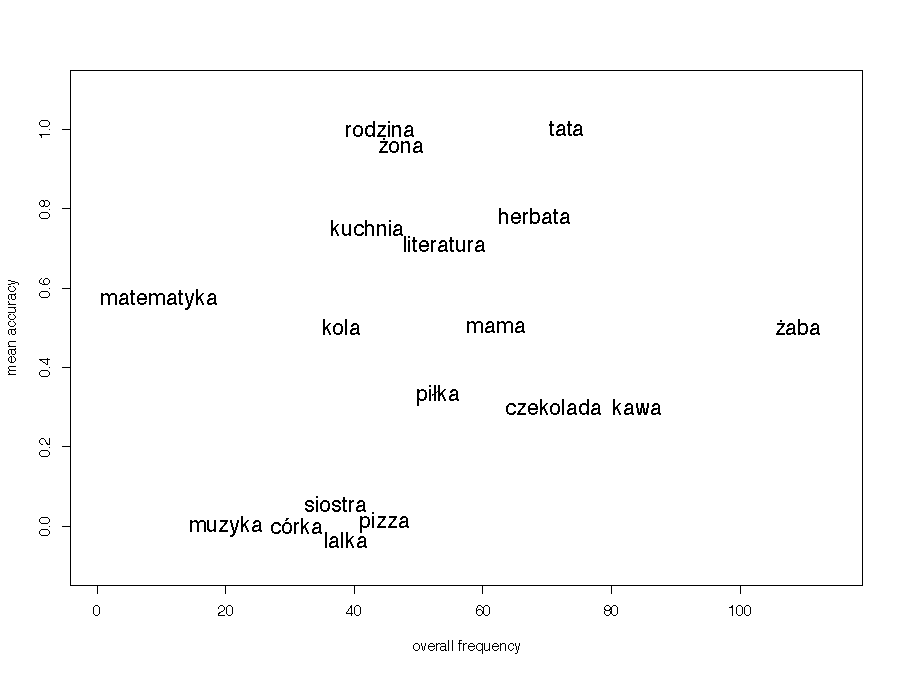
\includegraphics[width=\textwidth]{figures/07-2.pdf}
    \caption{Semi-spontaneous production task: mean accuracy / overall frequency}
    \label{fig:07:2}
\end{figure}

To conclude this section, it is worthwhile to point out that many of the words discussed in the analysis are fairly infrequent in the output data, as they were only produced by as few as a single learner. Tendencies regarding the properties of lexical items thus interact with the performance of individual learners, to which the next section is devoted. In any case, the analysis just concluded highlighted no obvious relation between input and output, in spite of the strong tendencies identified in the input (\chapref{sec:3}).

\subsection{Same-word utterances}\label{sec:07:2.2}

This section discusses case-marking variability within the same lexeme in the output of individual learners. The question may be pursued by looking at the output of participants with a mean accuracy different from 0 or 1, and in which the same lexical item occurs more than once (\tabref{tab:07:22}). If the rule governing case marking is simply unstable, then repeated lexical items should appear sometimes in their nominative, sometimes in their accusative form, with no apparent logic. If, on the other hand, case marking obeys a systematic principle, then each item should always appear in the same word-form in the same syntactic context.

\begin{table}
    \fittable{
    \begin{tabular}{lll}
        \lsptoprule
        participant & utterance & Lexeme\\
        \midrule
        5102 & [i ɔna lubi literature]. & [literature]\\
        5102 & [i ɔn lubi matematike literature]. & [literature; matematike]\\
        5102 & [i lubi matematike]. & [matematike]\\
        5102 & [i kɔxa ʒɔne eve i kɔta i kɔta i psa]. & [ʒɔne; eve]\\
        5102 & [i ɔn ma ʒɔne eve]. & [ʒɔne; eve]\\
        5104 & [on ma kɔta i sən i tsurka]. & [tsurka]\\
        5104 & [ɔn ma sən i tsurka i fortɛpjan]. & [tsurka]\\
        5109 & [ɔna lubi kava ərbate leteratura]. & [kava; ərbate; leteratura]\\
        5109 & [on lubi literatura i matematike]. & [literatura; matematike]\\
        5109 & [ɔn lu ɔn lubi literature matematike]. & [literatura; matematike]\\
        5109 & [ɔna lubi kava i korvate ʧekolada]. & [kava; korvate; ʧekolada]\\
        5109 & [ɔn lubi lɔde ʧekolada i korvatje]. & [ʧekolada; korvatj]e\\
        5113 & [ɔna lubi literatura kave i i kɔt]. & [literatura; kave]\\
        5113 & [i lubi literatura i kino i kerbate i kava i psa i kot]. & [literatura; kerbate; kava]\\
        5115 & [kristina xoxa mama mame]. & [mama mame]\\
        \lspbottomrule
    \end{tabular}
    }
    \caption{Same-word utterances}
    \label{tab:07:3}
\end{table}

A few cases (e.g. the single utterance of learner 5115) are evident instances of disfluencies and self-corrections. Other learners exhibit a more variable picture of case-marking with the same lexical items. 5109 produces three instances of \textit{literatur-a}, ‘literature-\textsc{nom}’, and one of \textit{literatur-ę}, ‘literature-\textsc{acc}’; 5113 produces one instance of \textit{kaw-a}, ‘coffee-\textsc{nom}’, and one of \textit{kaw-ę}, ‘coffe-\textsc{acc}{}'.

With only these three exceptions, all other lexical items always occur in the same word-form, which can be indifferently -/e/ ACC (in the speech of learner 5102) or, more commonly, -/a/ NOM. 

\section{Evaluating a syntactic principle of utterance organisation}\label{sec:07:3}

In the following section, the statistical tool introduced in \chapref{sec:3} will be applied to the production data discussed in this chapter in order to verify whether or not learners use inflectional morphology in a target-like and systematic manner, that is, following a morphosyntactic principle.

It is worthwhile to start with an overview of the data-set. \tabref{tab:07:4} reports the lexemes produced by each participant in the ACC form. Not all learners produced all lexemes: the number of participants producing each lexeme ranges from a minimum of 1 (e.g. \textit{żona,} ‘wife’) to a maximum of 11 for \textit{literatura}, ‘literature’. 

\begin{table}
\fittable{
    \begin{tabular}{ll}
        \lsptoprule
                participant & lexemes\\
        5101 & \textit{czekolada,} \textit{kuchnia,} \textit{literatura,} \textit{siostra}\\
        5102 & \textit{córka,} \textit{Ewa,} \textit{literatura,} \textit{matematyka,} \textit{piłka,} \textit{siostra,} \textit{żaba,} \textit{żona}\\
        5104 & \textit{córka,} \textit{lalka,} \textit{literatura}\\
        5105 & \textit{Herbata}\\
        5106 & \textit{czekolada,} \textit{herbata,} \textit{kawa,} \textit{kola,} \textit{literatura}\\
        5107 & \textit{córka,} \textit{herbata,} \textit{kawa}\\
        5109 & \textit{chorwacja,} \textit{czekolada,} \textit{herbata,} \textit{kawa,} \textit{kuchnia,} \textit{literatura,} \textit{matematyka}\\
        5111 & \textit{herbata,} \textit{literatura}\\
        5112 & \textit{kuchnia,} \textit{literatura,} \textit{pizza} \\
        5113 & \textit{czekolada,} \textit{herbata,} \textit{kawa,} \textit{literatura,} \textit{żaba}\\
        5114 & \textit{Anna,} \textit{czekolada,} \textit{herbata,} \textit{kola,} \textit{piłka}\\
        5115 & \textit{córka,} \textit{literatura,} \textit{mama,} \textit{matematyka,} \textit{tata}\\
        5116 & \textit{literatura,} \textit{rodzina}\\
        5117 & \textit{herbata,} \textit{kawa,} \textit{literatura,} \textit{matematyka}\\
        5118 & \textit{córka,} \textit{matematyka,} \textit{muzyka}\\
        5119 & \textit{czekolada,} \textit{herbata,} \textit{kawa,} \textit{piłka}\\
        \lspbottomrule
    \end{tabular}
    }
    \caption{Lexemes produced by learners}
    \label{tab:07:4}
\end{table}

One can now proceed to verify what principle of utterance organisation each learner may be thought to have adopted. The analysis will only focus on those participants who produced at least three occurrences of a feminine noun in the object function. \tabref{tab:07:5} indicates the following information: mean score (“mean”); number of correctly case-marked feminine nouns (“correct”); overall number of feminine nouns produced (“contexts”); number of lexical types produced (“lexemes”); ratio between number of utterances and number of lexical types, in which a value of 1 indicates that each lexeme occurs in only one utterance, while higher values indicate that at least some occur more than once. The last three parameters are useful to obtain a more complete picture of the interlanguage: while high mean scores might suggest that the learner has mastered the L2 morphosyntactic system, a reduced number of utterances might lead to questioning this claim. By the same token, few lexemes might suggest that the learner is not applying a rule, but only replicating chunks extracted from the input and not necessarily analysed in terms of morphosyntax. Following the approach described in detail in \chapref{sec:4}, the last column indicates the probability that learners achieved the observed scores or higher if they were not applying a systematic morpho-syntactic principle.

\begin{table}
    \begin{tabularx}{\textwidth}{lrrrrrr}
        \lsptoprule
         participant & mean & correct & contexts & lexemes & utterances/lexemes & p\\
         \midrule
         5101 & 0.67 & 4 & 6 & 4 & 1.50 & 0.11\\
         5102 & 0.83 & 10 & 12 & 8 & 1.50 & < 0.01\\
         5104 & 0.25 & 1 & 4 & 3 & 1.33 & 0.69\\
         5106 & 1.00 & 8 & 8 & 5 & 1.60 & < 0.01\\
         5107 & 0.33 & 1 & 3 & 3 & 1.00 & 0.50\\
         5109 & 0.46 & 6 & 13 & 7 & 1.86 & 0.50\\
         5112 & 0.67 & 2 & 3 & 3 & 1.00 & 0.13\\
         5113 & 0.43 & 3 & 7 & 5 & 1.40 & 0.50\\
         5114 & 0.20 & 1 & 5 & 5 & 1.00 & 0.81\\
         5115 & 0.33 & 2 & 6 & 5 & 1.20 & 0.66\\
         5117 & 0.50 & 2 & 4 & 4 & 1.00 & 0.31\\
         5118 & 0.00 & 0 & 3 & 3 & 1.00 & 0.88\\
         5119 & 0.00 & 0 & 8 & 4 & 2.00 & 1.00\\
        \lspbottomrule
    \end{tabularx}
    \caption{Semi-spontaneous production task, morphosyntactic principle probability by learner}
    \label{tab:07:5}
\end{table}

A few learners have a p value close to 0, which seems to suggest a systematic use of the target morphosyntactic principle. Learner 5106 made no errors at all; regarding 5102, the passage in which her two errors occur is reported in \REF{ex:07:8}:\todo{*STU's are actually to the left of the examples}

\ea%8
    \label{ex:07:8}
    \ea{\label{ex:07:8a}
    \gll    [ɔna   ɔn   ma  brat-a].\\
            \hspaceThis{[}she  he  has  brother-\textsc{acc}\\}\jambox*{*STU}
    \glt    ‘She has (a) brother.’
    \ex{\label{ex:07:8b}
    \gll    [ma   siostr-a].\\
            \hspaceThis{[}has  sister-\textsc{nom}\\}\jambox*{*STU}
    \glt    ‘(She) has (a) sister.’
    \ex{\label{ex:07:8c}
    \gll    [i  ma  dzurk].\\
            \hspaceThis{[}and  has  daughter.?\\}\jambox*{*STU}
    \glt    ‘And (she) has a daughter.’
    \z
\z

No convincing explanation could be found for the item [dzurk]. Apart from the examples just discussed, learner 5102 proved fairly accurate over a wide range of utterances and lexical items. 

At the other end of the spectrum, two learners (5118 and 5119) did not produce any accusative marking (three and eight obligatory contexts, respectively). All nouns probably occur in a single invariable word-form in -/a/ and morphological variation does not take place.

All other cases present a somewhat mixed picture. Thresholds are intrinsically arbitrary, which is why p values are presented in \tabref{tab:07:5} instead of a binary classification, as was done, on practical grounds, in the chapters devoted to the structured tests. For reasons of consistency with the previous analysis, though, 10\% can be taken as a working threshold. P values below this figure indicate that the probability of rejecting the null hypothesis (learners achieved the observed results without systematically applying a morphosyntactic principle) when this is in fact true is lower than 10\%.

Regarding the participants whose p values are above 0.1, it cannot be firmly asserted that they systematically mark all feminine nouns with the object function as accusative, as required by the target language. Nonetheless, they sometimes do, which witnesses to the fact that they must have noticed some morphological variation in the input, identifying the word forms in which lexical items may appear. What is still missing is the ability to use the correct word-form in the appropriate syntactic context, that is, a form-function association between syntactic function and word-form. 

\section{Correlating the structured tests with semi-spontaneous output}\label{sec:07:4}

A further question may be whether or not the learners’ morphosyntactic skills differ depending on the task through which they are elicited. The previous chapters described learner performance as observed in a structured test, while the present analysis focuses on semi-spontaneous production. The two contexts are quite different from each other in at least two respects. First, the structured tests present an ideal, yet artificial environment for the use of the target structure, while the production task recreates a realistic communicative situation in which the L2 is used not as part of an exercise, but in order to achieve some goal. Secondly, the production task may appear more complex from a cognitive point of view, which in some models, like \citegen{SkehanFoster2001} Limited Attentional Capacity Model, should produce poorer performance because of the dispersion of attentional resources it brings about. Therefore, the present research question may be summarised as “what can learners do in a realistic communicative situation given their results in the structured tests, which should elicit their very best theoretically possible performance?”. 

For each participant who produced at least three obligatory contexts, \tabref{tab:07:6} presents the p-value computed in the preceding section, representing the probability of observing this proportion of correct case marking or higher if the learner is \textit{not} applying a morphosyntactic principle. The last column reports the learners’ global score in the structured tests after comparable input exposure (T1), expressed in terms of scenarios (see \chapref{sec:6}).

\begin{table}
    \begin{tabularx}{\textwidth}{lrr}
        \lsptoprule
         participant & semi-spontaneous production p & structured task scenario\\
         \midrule
         5102 & < 0.01 & 1;1\\
         5101 & 0.11 & 1;1\\
         5112 & 0.13 & 1;1\\
         5113 & 0.50 & 3;1\\
         5118 & 0.88 & 3;1\\
         5117 & 0.31 & 2;1\\
         5115 & 0.66 & 2;1\\
         5119 & 1.00 & 2;1\\
         5107 & 0.50 & 2;3\\
         5114 & 0.81 & 2;3\\
         5106 & < 0.01 & 4;1\\
         5109 & 0.50 & 4;1\\
         5104 & 0.69 & 4;1\\
        \lspbottomrule
    \end{tabularx}
    \caption{Correlation between spontaneous interaction and structured tests}
    \label{tab:07:6}
\end{table}

All participants with a p value below 10\% belong to scenario 1;1. It thus seems that in order to be able to systematically produce case inflection in spontaneous production, a learner must be able to process SO and OS targets in both the EI and the comprehension test, although as mentioned no OS utterance was observed in the production task. Even learners who successfully repeated the ACC ending in the SO, but not OS targets of the EI test failed to do so in their spontaneous output.

\section{Interlanguage principles of utterance formation and interpretation}\label{sec:07:5}

The analysis so far has shown that only a minority of participants consistently uses morphology to express meaning in their semi-spontaneous output: yet all of them managed to successfully complete their task. On what principles did they rely then to express and decode meaning? The following qualitative analysis aims to identify the linguistic means which allow learners to successfully identify or express the intended meaning.

Most often, the referents involved in the utterance differ in their animacy, whereby the animate referent has the greatest probability of being the experiencer \REF{ex:07:9a}. When referents do not differ in their animacy, default SO word order can be relied on \REF{ex:07:9b}. In fact, the entire corpus of learner output does not contain a single OS utterance, although it could be argued that such structures were simply not required pragmatically.

\ea%9
    \label{ex:07:9}
    \ea{\label{ex:07:9a}
    \gll    [ʤulj-a  lubi  herbat-e   kol-a    i  ʧokolad-a]\\
            \hspaceThis{[}Giulia-\textsc{nom}  likes  tea-\textsc{acc}   coke-\textsc{nom}  and  chocolate-\textsc{nom}\\}\jambox*{(5114)}
    \glt    ‘Giulia likes tea, coke and chocolate.’
    \ex{\label{ex:07:9b}
    \gll    [luk-a    xoxa  hann-a].\\
            \hspaceThis{[}Luca-\textsc{nom}  loves  Anna-\textsc{nom}\\}\jambox*{(5114)}
    \glt    ‘Luca loves Anna.’
    \z
\z

Animacy contrasts  and default word order structure the output of all learners, even of those who appear to be able to use inflectional morphology productively \REF{ex:07:10}.

\ea%10
    \label{ex:07:10}
    \ea{\label{ex:07:10a}
    \gll    [ɔna  lubi  literatur-e]. \\
            \hspaceThis{[}she  likes  literature-\textsc{acc}\\}\jambox*{(5102)}
    \glt    ‘She likes literature.’
    \ex{\label{ex:07:10b}
    \gll    [i  ɔn  ma  ʒɔn-e    ev-e]\\
            \hspaceThis{[}and  he  has  wife-\textsc{acc}  Ewa-\textsc{acc}\\}\jambox*{(5102)}
    \glt    ‘And he has a wife, Ewa.’
    \z
\z

The same principles operate in native speech as well, as witnessed by the input analysis presented in \sectref{sec:3}. The vast majority of transitive utterances involves both a contrast in animacy and default SO word order \REF{ex:07:11a}; if the utterance has an OS structure, \REF{ex:07:11b}, animacy still ensures that meaning can be easily decoded. In case there is more than one animate referent \REF{ex:07:11c}, correct decoding may rely on SO word order alone. Only in a minority of utterances is morpho-syntactic analysis indispensable to decode meaning correctly, as both referents share the same value of animacy in the presence of marked word order \REF{ex:07:11d}.

\ea%11
    \label{ex:07:11}
    \ea\label{ex:07:11a}
    \gll    {Filip}    {pcha}    {wózek}.\\
            Filip\textsc{.nom}  pushes  cart\textsc{.acc}\\
    \glt    ‘Filip pushes the cart.’
    \ex\label{ex:07:11b}
    \gll    {muzyk-ę}  {lubi}  {Leon}.\\
            music-\textsc{acc}  likes  Leon\textsc{.nom}\\
    \glt    ‘Leon likes music.’
    \ex\label{ex:07:11c}
    \gll    {mąż}      {kocha}  {żon-ę}.\\
            husband\textsc{.nom}  loves  wife-\textsc{acc}\\
    \glt    ‘The husband loves (his) wife.’
    \ex\label{ex:07:11d}
    \gll    {brat-a}    {kocha}  {Juli-a}.\\
            brother-\textsc{acc}  loves  Julia-\textsc{nom}\\
    \glt    ‘Julia loves (her) brother.’
    \z
\z

\section{Summary}\label{sec:07:6}

This chapter aimed at analysing semi-spontaneous speech in interaction, elicited through a task in which learners spontaneously produced a good number of target structures, namely feminine nouns in transitive sentences.

The analysis shows that the subject is always expressed by a name (e.g. \textit{Anna}) or a pronoun (e.g. \textit{ona}, ‘she’), never by a common noun (e.g. \textit{aktorka}, ‘actress’) as was the case in the two structured tests. The object is most often represented by an inanimate noun (e.g. \textit{herbata}, ‘tea’). Animate (e.g. \textit{pies} ‘dog’) and human (e.g. \textit{córka}, ‘daughter’) are relatively rare. This partly reflects the input learners were exposed to (see \sectref{sec:6}), in which, based on their semantics, specific lexical items are more likely to perform the subject or object syntactic function.

In spite of this uneven distribution in the input, the accuracy of morphosyntactic marking does not appear to depend on the relative frequency of accusative word forms on the total occurrences of a lexeme. The output of those learners who repeat the same lexemes more then once showed that alongside limited variability, the same word tends to occur in the same word-form when it is repeated. Although this observation seems to suggest that learners memorised the lexical item in a specific word form, the limited amount of data does not allow for any generalisations.

The statistical analysis of case-marking shows that only a few learners inflect nouns with above chance accuracy. Most of the learners who performed above chance in interaction also succeeded in both tests and with both word orders. It thus seems that being able to manipulate word order and case marking in comprehension and repetition is a prerequisite for correctly inflecting nouns in interaction, albeit with unmarked word order only.

The qualitative analysis of learner output shows that, independently on the accuracy with which case-marking is produced, utterances are shaped by animacy contrasts and default SO word order. The combination of these two principles is sufficient to express the meaning required in the task. Indeed, the vast majority of input utterances can be interpreted on their basis as well.

\chapter{Discussion}\label{sec:7}

The present chapter summarises and discusses the results obtained in the preceding chapters.

\section{Input}\label{sec:08:1}

This chapter aimed to scrutinise the controlled VILLA input in order to appropriately contextualise the learner task in the linguistic tests discussed later on in the book.

The analysis of the association between case endings and the corresponding syntactic functions showed that, indeed, the ending -[a] is more strongly linked to the SUBJ function than the ending -[e] is linked to the OBJ function. This might play a role in justifying why learners hardly ever process the nominative case incorrectly, while errors concerning the accusative case are quite common. 

Further, while the object function was characterised by relatively high type variety, with numerous inanimate nouns performing it, the subject function is instantiated by only four macro-types, namely the two personal pronouns \textit{on} and \textit{ona}, ‘he’ and ‘she’, and masculine and feminine person names. The high type variety of the object function might explain why some learners managed to correctly inflect in the accusative case even nouns which never appeared in that form in the input. However, since the VILLA project was not designed to investigate this particular research question, it is impossible to pursue it any further based on the present data. 

The input was then scanned for all possible sentence models, described in terms of the combination of the following parameters:

\begin{itemize}
    \item word order: SO vs. OS;
    \item subject word class: personal pronoun, person name, common noun;
    \item object word class: person name, common noun;
    \item subject and object gender: masculine vs. feminine;
    \item animacy (animate vs. inanimate).
\end{itemize}

Not surprisingly, only a fraction of the 96 theoretically possible patterns were attested in the input. The trends highlighted by the analysis of type frequency were confirmed: the subject tends to be instantiated by personal pronouns or person names, while the object shows a privileged association with inanimate nouns. The target structures of the two structured tests are rare or absent altogether from the input when all parameters are considered: however, figures markedly rise when a morphological perspective is adopted, whereby word class and animacy are ignored (when legitimate) and patterns are considered as mere sequences of inflectional endings occurring in a given order.

The following sections aim to add a few details which may not emerge sufficiently from an exclusively quantitative analysis, such as the effect of information structure on the frequency of selected morphosyntactic structures. It further discusses the implications of the input distribution just reviewed for the learner task.

\subsection{information structure}\label{sec:08:1.1}

The VILLA input was designed to allow for rigorous experimental control over a large set of variables, but at the same time it was delivered in the form of a communicative, interactive language course. In order not to sound unnatural, the teacher would inevitably produce the structures which she judged pragmatically most appropriate, even if these were \textit{not} the structures targeted in the language tasks. To exemplify, in a context in which the same known characters are mentioned over and over again, it is pragmatically appropriate to refer to them using personal pronouns or their names, like \textit{ona} ‘she’ or \textit{Julia}, rather than a common noun indicating their nationality of profession, like \textit{kucharka} ‘cook’. Together with the structure and contents of the course, this pragmatic constraint led to a very low frequency of constructions targeted in the VILLA structured tests, which exclusively include common nouns.

Across all models of transitive structures, pronouns and person names represent the lion's share as far as the expression of the subject function is concerned, while objects are mainly instantiated by inanimate nouns. This trend is not surprising if one considers the topics covered throughout the course, which for the most part described a handful of human characters along with their likes and dislikes and their relation with each other. Human referents clearly have the greatest chances of being the subject of transitive sentences for obvious extralinguistic reasons. The distribution of pronouns and person names to refer to the same human referent, in contrast, is regulated by information structure. In a typical VILLA input sequence, pronouns are commonly used to refer to entities which have been previously introduced using a person name \REF{ex:08:1}, although such topic maintenance is also frequently achieved by repeating the character’s name as well.

\ea%1
    \label{ex:08:1}
    \ea{\label{ex:08:1a}
    \gll    {Juli-a} {lubi} {żółwi-a.}\\
            Julia-\textsc{nom}  likes  turtle-\textsc{acc}\\}\jambox*{TEA*}
    \glt    ‘Julia likes the turtle.’
    \ex{\label{ex:08:1b}
    \gll    {ona}   {lubi}   {lizaki}     {lubi}   {lizaki.}\\
            She  likes  lollipops\textsc{.acc}   likes  lollipops\textsc{.acc}\\}\jambox*{TEA*}
    \glt    ‘She likes lollipops.’
    \ex{\label{ex:08:1c}
    \gll    {ona}   {lubi}   {żółwi-a}   {i}   {lubi}   {czekolad-ę.}\\
            She  likes  turtle-\textsc{acc}  and  likes  chocolate-\textsc{acc}\\}\jambox*{TEA*}
    \glt    ‘She likes turtle and chocolate.’
    \z
\z

Entities are mainly introduced using person names rather than common nouns for reasons related to discourse. This claim can be best instantiated on the grounds of the context in which the class is working on the PowerPoint slide in \figref{fig:08:1}, trying to decide what course character likes or owns each of the objects depicted therein. 

\begin{figure}
    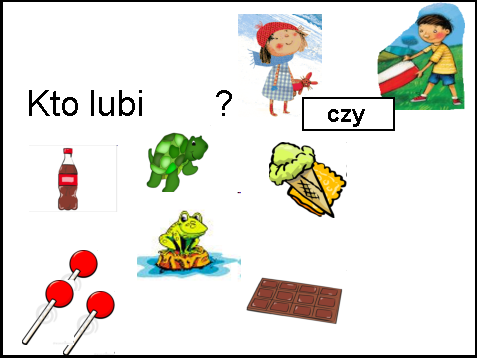
\includegraphics[width=\textwidth]{figures/08-1.pdf}
    \caption{PowerPoint slide from the VILLA input}
    \label{fig:08:1}
\end{figure}

Based on information previously provided during the lesson, the learners can decide between Julia and Filip (top right), both well known course characters. In this particular communicative context the objects represent the discourse topic, while the two children are in the focus position. The sequence opens with the utterances in \REF{ex:08:2}:

\ea%2
    \label{ex:08:2}
    \ea{\label{ex:08:2a}
    \gll    {kto}   {lubi}   {czekolad-ę}?\\
            who   likes   chocolate-\textsc{acc}?\\}\jambox*{TEA*}
    \glt    ‘Who likes chocolate?’
    \ex\label{ex:08:2b}
    {eh}   {Gaston}\footnote{Gaston is the pseudonym of one of the learners.}?\hfill TEA*
    \ex{\label{ex:08:2c}
    \gll    {tak}   {Juli-a}     {lubi}   {czekolad-ę.}\\
            Yes  Julia-\textsc{nom}  likes  chocolate-\textsc{acc}\\}\jambox*{TEA*}
    \glt   ‘Yes, Julia likes chocolate.’
    \ex{\label{ex:08:2d}
    \gll    {czekolad-ę}     {lubi}   {Juli-a.}\\
            chocolate-\textsc{acc}  likes  Julia-\textsc{nom}\\}\jambox*{TEA*}
    \glt    ‘Julia likes chocolate.’
    \z
\z

The teacher first asks Gaston who likes chocolate, whether Julia or Filip. Input transcription at this stage is only available for the teacher's speech and does not comprise the learner's response, but only teacher feedback. Judging on the teacher's third turn, however, Gaston's answer must have been correct, at least in terms of content; in any case, the teacher repeats (or recasts) the learner’s response. Even though the topic \textit{czekoladę} ‘chocolate-\textsc{acc’} performs the object function, thus licensing syntactically marked word order, the native speaker at first prefers to produce a syntactically unmarked SO sentence, in which pragmatic markedness is expressed prosodically through the stressing of utterance-initial \textit{Julia}, which highlights her as the sentence focus. Only later will the teacher produce the equivalent OS utterance.

Judging on the apparent interchangeability of the two word orders, one may wonder if learners even deemed it necessary to pay attention to such syntactic devices, since different syntactic structures correspond to identical meaning. Speakers of languages which also allow the functional manipulation of word order, like German and, with different means, Italian, might even have found this apparently random use of syntactically marked structures a little odd. On the other hand, the school-like context in which the project was carried out might have prompted students to pay attention to these details of the target grammar even if it seemed difficult to associate competing forms to the corresponding meaning.

This example is precious to understand two important points. First, not only are OS sentences more marked than their SO equivalents, but their purpose can be easily (and perhaps, preferably) fulfilled by other strategies to mark departures from the default alignment between the syntactic and pragmatic structure of the utterance (topic-subject; focus-object).

On the other hand, the example clarifies why person names are so much more frequent than common nouns in transitive structures. Teacher speech is mainly based on PowerPoint slides which depict the same characters over and over again. Thus, even if each course character is identified by a particular nationality and profession, expressed in turn by common nouns, the course characters become so familiar that it would seem somewhat unnatural to refer to them otherwise than by their name, for instance by saying \textit{dziewczynka} ‘little girl’ instead of just \textit{Julia}. In contrast, the target sentences of the EI task required learners to process common nouns in the absence of any context, something which they could arguably be ill-equipped to do at such an early stage of acquisition and on the sole basis of the input just described.

\subsection{Form-function association}\label{sec:08:1.2}

The analysis of form-function associations has shown that, based on a statistical analysis of the input, it is simpler to associate [a] to the subject function than [e] to the object functions. Before moving on to a more detailed discussion of the mechanisms of such an analysis, it seems worthwhile to point out a few important details which may prove helpful to provide a more comprehensive picture of the learner’s task in the VILLA project.

The first is that while subconscious input analysis and associative learning certainly play a role in SLA, there are many other factors which may concur to explain learner behaviour. As far as the nominative case in [a] is concerned, for instance, it most often coincides with the citation form of lexical items, i.e. the form which was usually introduced first throughout the course and which was used out of context. To exemplify, \textit{kuchnia} ‘cuisine’ is a noun which due to its semantics tends to occur in the accusative case, yet, its basic word form is modelled on the nominative case: in example \REF{ex:08:3}, the teacher first uses the noun in the accusative case, then asks the class to repeat it aloud in the nominative.

\ea%3
    \label{ex:08:3}
    \ea{\label{ex:08:3a}
    \gll    {ona}   {lubi}   {kuchni-ę}   {włosk-ą.}\\
            she  likes  cuisine-\textsc{acc}  Italian-\textsc{acc}\\}\jambox*{TEA*}
    \glt    ‘She likes Italian cuisine.’
    \ex{\label{ex:08:3b}
    \gll    {proszę}   {mówić}   {kuchni-a}   {włosk-a.}\\
            please  say  cuisine-\textsc{nom}  Italian-\textsc{nom}\\}\jambox*{TEA*}
    \glt    ‘Please say Italian cuisine.’
    \z
\z

Similar factors, while not quantitative in nature (a word initially introduced in the nominative case may be then used predominantly in the accusative case, e.g. \textit{herbata} ‘tea’) certainly contribute to the prominence (here understood as the possibility of remembering it) of one or another form. 

Further, widespread morphological syncretism may hinder the univocal identification of form-function associations. In perfectly legitimate sentences like \REF{ex:08:4a} and  \REF{ex:08:4b}, nouns performing different syntactic functions are marked by the same inflectional ending [a] because they belong to different inflectional paradigms. Curiously, in this respect such utterances resemble those produced in the EI test by learners who cannot yet manipulate inflectional morphology (\ref{ex:08:4c}, here transcribed in standard orthography).

\ea%4
    \label{ex:08:4}
    \ea\label{ex:08:4a}
    \gll    {siostr-a}   {woła}   {brat-a} \\
            sister-\textsc{nom} calls   brother-\textsc{acc}\\
    \ex\label{ex:08:4b}
    \gll    {ona}   {ma}   {brat-a.}\\
            she  has  brother-\textsc{acc}\\
    \ex[*]{\label{ex:08:4c}
    \gll    {dziewczynk-a}   {ciągnie} {portugalk-a}\\
            little.girl-\textsc{nom}  pulls   Portuguese.woman-\textsc{nom}\\}
    \glt   
    \z
\z

The two models can only be distinguished based on the grammatical gender and animacy of the two nouns involved, because the endings they exhibit are formally identical. This may easily confuse learners, as it adds a further factor to take into consideration when computing the form-function association between case endings and syntactic functions: not only is the syntactic function relevant, but grammatical gender also needs to be accounted for. This in turn is not predictable, although in the case of human nouns it almost always coincides with biological sex. There are exceptions to this rule, though: in \REF{ex:08:5}, both the subject and the object are realised by nouns inflected according to the feminine paradigm, namely \textit{córka}, ‘daughter’ and \textit{tata}, ‘Dad’. The latter, however, is semantically masculine. Nevertheless, it should be pointed out that although fairly frequent, the word \textit{tata} is the only lexical item characterised by such properties.

\ea%5
    \label{ex:08:5}
    \gll    {córk-a}     {Juli-a}     {kocha} {tat-ę.}\\
            daughter-\textsc{nom}  Julia-\textsc{nom}  loves  dad-\textsc{acc}\\
    \glt    ‘(The) daughter Julia loves (her) father.’
    \z

A further point of complexity in the VILLA input is represented by the fact that in Polish the default case of direct objects under the scope of negation is not the accusative, as one would expect, but the genitive. In the paradigm of masculine animate nouns, the [a] ending characterises both the accusative case and the genitive \REF{ex:08:6a}. In the feminine paradigm, on the contrary, the two endings are clearly distinct, so that direct objects are marked by different case endings depending on whether or not their verb is negated \REF{ex:08:6b}. Finally, the genitive is also the case in which the subject appears when an existential verb is negated \REF{ex:08:6c}.

\ea%6
    \label{ex:08:6}
    \ea\label{ex:08:6a}
    \gll    {nie}   {ona}   {nie}   {kocha}   {dziadk-a}   {Karol-a.} \\
            no  she  not  loves  grandpa-\textsc{gen}  Karol-\textsc{gen} \\
    \glt    ‘No, she doesn't love grandpa Karol.’
    \ex\label{ex:08:6b}
    \gll    {babcia}   {nie}   {lubi}   {muzyk-i.}\\
            grandmother  not  likes  music-\textsc{gen}\\
    \glt    ‘Grandmother doesn't like music.’
    \ex\label{ex:08:6c}
    \gll    {nie}  {ma}  {Karol-a}\\
            not  has  Karol-\textsc{gen}\\
    \glt    ‘Karol is not here.’
    \z
\z

The last example is crucial in that it confuses the relation between syntactic function and inflectional ending. These regularities are quite systematic and easily described if basic meta-linguistic concepts and rules are introduced, but the VILLA input included no such explanations. 

Another important point concerns the selection of the meaning engaged in the form-function association. In the present analysis “subject” and “object” were chosen because they correspond most accurately to the meaning expressed in Polish by the morphemes [a] and [e], respectively. There is no guarantee that the learner identified the same relation, however: in fact, it may be argued that such top-down expectations resemble \citegen{Bley-Vroman1983} comparative fallacy, whereby the interlanguage is analysed not in terms of its internal organisation, but of the target it is supposed to imitate. In fact, different learners may assign different meaning to the same morpheme. \citet{Bernini2018a} and \citet[28-33]{Dimroth2018} both discuss two forms of the word \textit{strażak} ‘fireman’ as can be encountered in narrations produced within the Italian and German VILLA editions, respectively, whereby a form in \textit{{}-k} (e.g. [ˈstraʒak]) modelled on the nominative case opposes a form in \textit{{}-em} (e.g. [straˈʒakjem]), modelled on the instrumental case \textit{strażakiem}. In the Italian data, the opposition seems to vehiculate the functions “subject/controller” vs. “oblique”, while in the German data a “singular” vs. “plural” seems more probable.

The learner’s task is further complicated by the differential object marking (DOM) encountered in the masculine paradigm. Nouns referring to things appear in a form identical to the nominative case, characterised by a zero morph attached to the consonantal stem (\ref{ex:08:7a} and \ref{ex:08:7c}), while the accusative case of masculine animate nouns \REF{ex:08:7b} present an [a] ending \REF{ex:08:7d}, which is also found in the genitive case \REF{ex:08:7e}. This last observation highlights the fact that DOM complicates the association between form and function on metalinguistic, rather than statistical grounds: on hearing the two forms in \REF{ex:08:7d} and \REF{ex:08:7e}, the learner can be hardly expected to identify a comprehensive morphosyntactic rule, especially in the absence of an understanding of the category of case and detailed information as to Polish inflectional morphology. It must be said, however, that all VILLA L1s except German do not inflect nouns for case, so that encountering the same word form in different syntactic functions should not be particularly problematic for speakers of these languages. Nonetheless, the typological difference between the VILLA L1s and Polish is quite evident and a provisional hypothesis should be formulated to account for it. 

\ea%7
    \label{ex:08:7}
    \ea\label{ex:08:7a}
    \gll    {to}    {jest}  {balonik{}-${\emptyset}$}\\
            this\textsc{.nom}  is  balloon\textsc{.m-nom}\\
    \ex\label{ex:08:7b}
    \gll    {to}    {jest}  {strażak-${\emptyset}$}\\
            this\textsc{.nom}  is  fireman\textsc{-nom}\\
    \ex\label{ex:08:7c}
    \gll    {Jan-${\emptyset}$    ma  balonik-${\emptyset}$}\\
            Jan\textsc{-nom}  has  balloon\textsc{.m-acc}\\
    \ex\label{ex:08:7d}
    \gll    {Jan-${\emptyset}$    zna  strażak-a}\\
            Jan\textsc{-nom}  knows  fireman\textsc{.m-acc}\\
    \ex\label{ex:08:7e}
    \gll    {to}    {jest}  {samochód-${\emptyset}$}  {strażaka}\\
            this\textsc{.nom}  is  car\textsc{-nom}  fireman\textsc{-gen}\\
    \z
\z

A final point concerns the form component. Discussing the form-function association between [e] and "object”, it was stated above that i) most feminine nouns in the accusative case are characterised by word-final -[e], and ii) only a small proportion of words in -[e] are indeed instances of ACC.SG.F. While i) seems unproblematic, ii) may not seem entirely adequate to model the learner’s task during input processing. This point begs the researcher to take a stance, depending upon the answer to the following question: when establishing form-function associations through contingency learning, can learners distinguish words sharing a given form, but belonging to obviously different word classes, and treat them in a different manner? Since in the tasks discussed in this work the VILLA learners were required to process nouns referring to human beings, one of their goals was to identify the forms (i.e. the inflectional endings) in which such words may appear, possibly attempting to discern any regularity governing their distribution. Thus, in the case of ACC.SG.F [e] one may wonder whether it is relevant to know how many input \textit{words} in -[e] really encode human nouns in the accusative case, or whether it is only relevant to know how many \textit{human nouns} in the input end in -[e]. 

In the former case, the learner will need to analyse all words in -[e] which comprise feminine nouns, indeed (e.g. \textit{portugalk-ę} ‘Polish.woman-\textsc{acc.sg’}), but also verbs (\textit{idzie} ‘go.\textsc{pres.3sg’}) adverbs (\textit{dobrze} ‘well’), adjectives (\textit{jakie} ‘which.\textsc{nom/acc.sg.n}’) and conjunctions (\textit{ale} ‘but’). Upon encountering a word in –[e], learners will (subconsciously) note whether or not it encodes the target meaning, in answer to the implicit question “how often do words in –[e] represent feminine human nouns in the object function?”.

In an alternative scenario, learners will separate nouns from all other categories and simply compute a list of the possible endings of human nouns along with their relative frequency (how many nouns with human referents are characterised by word-final –[e]? How many by –[a]? and so on).

The consequences of this decision for the estimation of form-function association are important. 

If learners are assumed to be able to distinguish word classes, then only a subset of input words sharing the form under investigation should be considered in the computation of form frequency, which will result in a higher form-function association index, all other things being equal. To exemplify, the range of words in -[e] relevant for the meaning “accusative case of feminine nouns” would comprise e.g. \textit{portugalk-ę} ‘Polish.woman-\textsc{acc.sg’}, but not \textit{idzie} ‘go.\textsc{pres.3sg}’, \textit{dobrze} ‘well’, \textit{jakie} ‘which.\textsc{nom/acc.sg.n}’ or \textit{ale} ‘but’, despite the fact that all share the form of interest -[e]. If learners cannot distinguish word classes, in contrast, then the same count should comprise any word in –[e].

In order to accurately acknowledge the fact that input processing may be selective, it seems appropriate to compute function > form associations based on language exemplars in which the meaning in question is present. From this perspective, the learner’s task is to identify how many feminine nouns in the object function  are characterised by word-final [e], and how many are not. 

When this rationale is applied to the VILLA data, the surprising results presented in \tabref{tab:08:1} and \tabref{tab:08:2} are obtained. Note that these tables are an elaboration of \tabref{tab:03:1} and \tabref{tab:03:2}, respectively, in which the columns no longer relevant have been shaded: in fact, following the approach adopted in this section, form-function association is simply the ration between the number of words including both form and function and the number of words encoding function regardless of form. Both association indexes are close to 1, which indeed reflects the fact that in the peculiar VILLA input most NOM.SG.F are characterised by word-final [a], and most ACC.SG.F are characterised by word-final [e].

\begin{table}
    \begin{tabularx}{\textwidth}{X>{\columncolor{lsDOIGray}}rrr >{\columncolor{lsDOIGray}}rr>{\columncolor{lsDOIGray}}r}
        \lsptoprule
        a & b & c & d & e & f & g\\
        \midrule
        L1 & {}-[e] & \textsc{Acc} \textsc{fem} & \textsc{Acc} \textsc{fem} -[e] & d/b & d/c & e*f\\
        EN & 6541 & 441 & 415 & 6.34\% & 94.10\% & 5.97\%\\
        FR & 3789 & 365 & 345 & 9.11\% & 94.52\% & 8.61\%\\
        GE & 6424 & 414 & 379 & 5.90\% & 91.55\% & 5.40\%\\
        IT & 7675 & 624 & 598 & 7.79\% & 95.83\% & 7.47\%\\
        NL & 6570 & 519 & 494 & 7.52\% & 95.18\% & 7.16\%\\
        \lspbottomrule
    \end{tabularx}
    \caption{Form > function index for syntactically relevant contexts only, ACC.SG.F [e]}
    \label{tab:08:1}
\end{table}

\begin{table}
    \begin{tabularx}{\textwidth}{Xrrr rrr}
        \lsptoprule
        a & b & c & d & e & f & g\\
        \midrule
        L1 & {}-[a] & \textsc{Nom} \textsc{fem} & \textsc{Nom} \textsc{fem} -[a] & d/b & d/c & e*f\\
        EN & 7091 & 2471 & 2437 & 34.37\% & 98.62\% & 33.89\%\\
        FR & 4239 & 1798 & 1730 & 40.81\% & 96.22\% & 39.27\%\\
        GE & 7100 & 2338 & 2265 & 31.90\% & 96.88\% & 30.91\%\\
        IT & 9345 & 3198 & 3161 & 33.83\% & 98.84\% & 33.43\%\\
        NL & 7483 & 2787 & 2721 & 36.36\% & 97.63\% & 35.50\%\\
        \lspbottomrule
    \end{tabularx}
    \caption{Form > function index for syntactically relevant contexts only, NOM.SG.F [a]}
    \label{tab:08:2}
\end{table}

This observation however is in stark contrast with the results of the tasks discussed in this work, which clearly show that [a] tends to be overextended onto [e] by a vast number of learners. It seems, therefore, that form-function association may not be the most influential factor to determine which input word-form will be selected as the basic word-form of the learner variety. Based on the tables presented above, raw token frequency appears to be a good candidate, as the instances of [a] NOM are almost six times as frequent as [e] ACC. Moreover, the nominative case appears in a much larger number of contexts than the accusative case, and is the default citation form of nouns. In sum, the approach adopted here in order to model learner selectivity in the computation of form-function association appears heavily biased by the fact that raw frequency is not taken into account. 

\subsection{A learner variety perspective}\label{sec:08:1.3}

As \citet{Dimroth2018} points out, it is often difficult to draw a line between the claims and predictions of the learner variety approach and usage-based theories. As far as the input is concerned, particularly, both consider it an essential component for interlanguage development, the raw material which the learner communication faculty will shape in order to reach the set communicative objectives.

From this perspective, inflectional morphology seems by no means indispensable to interpret input sentences, although it certainly is a characteristic and obligatory feature of the target language. It is not surprising then that learners can easily do without it and still communicate effectively, especially when a context is available. The analysis of learner’s semi-spontaneous productions has clearly shown that semantics (animacy) and default SO (controller – theme) word order are usually sufficient to express the simple meaning required in the VILLA tasks. 

The same trends are also commonly encountered in a vast proportion of input utterances: SO structures are preferred even in a language such as Polish, with its complex nominal morphology and the theoretical possibility to manipulate word order at will. By the same token, agents tend to be animate and patients tend to be inanimate simply because situations usually present this structure. In other words, the principles of utterance organisation in question may be seen as a feature of the basic variety, but are commonly encountered in most instances of verbal communication.

The models corresponding to the target sentences of the structured tests were either absent or rare in the input, precisely because they purposefully eliminate all natural cues to sentence organisation with the exception of inflectional morphology. From a communicative point of view, then, the EIT and the comprehension tasks are little more than exercises targeting meta-linguistic skills. The communicative principles of the basic variety are hardly applicable, but on the other hand it can be argued that there is hardly any meaning to express. 

Since the VILLA participants are all adult, competent speakers of at least one L1, one could argue that their experience in terms of pragmatics and world knowledge may sometimes prevail on the input received. As shown in a study conducted on copular structures \citep{Saturno2015}, learners often choose to ignore highly frequent input patterns, developing their own interlanguage structures instead. The copular construction with \textit{to} ‘this’, though extremely common in the input, appeared to be disfavoured both in a structured test and in semi-spontaneous production \citep{Saturno2018}. In the latter context, learners creatively elaborated new, ungrammatical constructions. The structure in \REF{ex:08:8a} probably has its models in \REF{ex:08:8b} and \REF{ex:08:8c}.

\ea%8
    \label{ex:08:8}
    \ea{\label{ex:08:8a}
    \gll    [ɔna   jɛst   dʒovanna].\\
            She  is  Giovanna\\}\jambox*{(5112)}
    \glt    ‘She is Giovanna.’
    \ex\label{ex:08:8b}
    \gll    {to}    {jest}  {Anna}\\
            this\textsc{.nom}  is  Anna\textsc{.nom}\\
    \ex\label{ex:08:8c}
    \gll    {Anna}  {jest}  {polką}\\
            Anna  is  Polish.woman\textsc{.ins}\\
    \z
\z

In sum, from the perspective of the learner variety approach the results of the linguistic tasks are not particularly unexpected. In the language tasks inflectional morphology is hardly encountered because it is not part of the repertoire of early interlanguages, which prefer to rely on semantics and word order. The same preferences contribute to shaping the input, too, although the latter obviously includes all obligatory traits of the target language, such as inflectional morphology. 

\section{The elicited imitation task}\label{sec:08:2}

Perhaps the most self-evident result emerging from the analysis of the Elicited Imitation Task (EIT) is that, as expected based on input analysis, the NOM ending [a] shows a marked tendency to overextend onto ACC [e]. For most participants, [a] is indeed the only ending produced, and thus the basic form of nouns, which – if one accepts the theoretical premises of the EI test – should clearly point to a positional principle of utterance organisation, whereby syntactic functions are determined by the relative position of nouns in the utterance.

A much smaller number of learners produce target-like output, in which the endings [a] and [e] alternate depending on the syntactic function of the noun. Such performance – again, based on the theoretical premises of the task – should indicate that the target language morphosyntactic principle of utterance organisation has been correctly identified and can be successfully reproduced in the output. Finally, a set of participants exhibits a variety of complex scenarios. 

Word order was found to exert a powerful role, whereby OS targets appear to cause greater difficulties than their SO equivalents. Time of exposure was also shown to be an important factor, whose predictable effect is an increase in performance from T1 from T2, with numerous learners moving closer to the target morphosyntactic principle of utterance organisation. An interaction with word order is observed, too: if partial improvement occurs, it is more likely to be on SO than OS targets. Finally, a weak but significant correlation was found between the LLama test and the score for the repetition of -/e/, averaged for time and word order.

Against this general picture, a few points remain partially unclear. They can be summarised as follows:

\begin{itemize}
    \item The range of observed case endings;
    \item Role of word order and processing for meaning;
    \item better performance on [e] than [a] targets;
    \item better performance at T1 than T2 targets.
\end{itemize}

It seems that all these issues ultimately depend on a precise understanding of the mechanism of the EIT, which is itself not completely clear. Therefore, the discussion will start with an attempt to identify the level of analysis into which the EI test may be thought to tap. 

\subsection{Range of case endings}\label{sec:08:2.1}

The range of case endings produced by the learners seems to be quite restricted. Such observation is not in accordance with studies on the morphological development in Slavic languages, which suggest that learners first go through a NOM/non-NOM opposition, and only later do they stabilise this generic contrast into a more target-like NOM/ACC distinction (see \chapref{sec:1}.

This does not necessarily mean that the VILLA learners acquired case marking better and more quickly than untutored SLA learners. The analysis of the VILLA semi-spontaneous production data by \citet{Bernini2016} and \citet{Dimroth2018} shows that utterance structure simultaneously reflects a variety of principles which in spontaneous SLA are typical of different developmental stages, such as the pre-basic variety’s pragmatic structure ``focus last''; the basic, semantic ``controller first''; and the post-basic SVO syntactic organisation. Interpreting such mixture of apparently anachronistic principles as a consequence of the particular VILLA learning context, one could propose the label ``Instructed Basic Variety''. Bernini in particular correlates the structural properties of the interlanguage with its phonology, arguing that while random phonological variability, or rather tolerance towards allophonic variation is typical of pre-basic varieties, ``la fixation d’une forme de base du […] mot dans la variété basique réduit la gamme de variation (allo-)phonique […], en fondant la possibilité d’oppositions phonémiques''. In this respect, he also observes that while several lexical items are relatively stable in their phonological form, others show considerable variability, both in their supposed target and in their phonetic structure, e.g. \{ɕpi, ʃpi, spi\} for target /ɕpi/, ‘sleeps’. Even when the various tokens produced by a learner seem to be mappable onto specific target forms, and thus to reflect the input to a certain extent, their use is nonetheless functionally differentiated, as it has been shown to be the case with spontaneous SLA (\citealt{BroederEtAl1993}). Moreover, Bernini suggests four factors which may have an influence in determining the phonological variability of lexical items in initial SLA, namely a) frequency, b) the number and structure of syllables, c) the number of different word-forms present in the input, and d) semantics. While b) and d) are intrinsic to the lexical items, a) and d) depend on the input. This wealth of data only makes it harder to interpret the output of the EI task, as even the correct repetition of case endings may indicate a post-basic syntactic utterance organisation just as well as pre-basic, random phonological variability. What appears to be incontrovertible is that learners must have picked these alternative endings from the appropriate input paradigms, thus showing some sensitivity to it. If one excludes the instances of centralised vowels mainly produced by the German learners, virtually all endings produced are instances of [a] or [e], despite the fact that the relevant paradigm also includes other salient and frequent endings, such as INS [o\~{w}]. This observation would witness to the fact that learners identified the syntactic context in which the endings [a] and [e] may occur, namely transitive sentences, and conversely that they are aware that in that syntactic context only those endings are allowed.

On the other hand, the fact that only [a] and [e] occur in the EI data is hardly surprising if one accepts that there might be repetition without processing, whereby learners only repeat what they hear without accessing their L2 grammar. In this situation, only two endings occur in the output simply because only those endings are present in the stimulus sentences.

\subsection{Sources of error: processing for meaning vs. perception}\label{sec:08:2.2}

Compared to previous studies using the EIT, the target structure of the present work introduces additional variables which increase the complexity of the analysis and interpretation of the data. Case marking poses different challenges from other target structures which only affect grammatical correctness, like for instance verb placement as studied by \citet{Håkansson1989} or \citet{Schimke2011}. Unlike case marking, the position of a verb in the utterance is not likely to change the overall meaning of the sentence. 

In addition, the data produced by the VILLA EIT are limited to the learner’s final output. In the absence of a comprehension or translation test, it is impossible to tell what learners meant to say. This is unfortunate, as the output of the EIT is the product of at least three complex processes, namely perception, comprehension and production: errors may lie at any level. By observing the learners’ processing of an OS target, for instance, one cannot tell if the underlying grammatical meaning was identified, firstly, and if any effort was made to reproduce it, secondly. It is also impossible to rigorously exclude that learners performed the task without processing targets for meaning. Indeed, this suspicion is further reinforced by the weak but significant correlation between phonological memory capacity as measure by the LLama test and the scores in the repetition of -/e/.

These questions were dealt with in detail in \chapref{sec:6}, in which the results of the EI and of the comprehension test were correlated in an attempt to provide a comprehensive picture of learners’ processing skills, and will be discussed further in \sectref{sec:08:4}. For the time being, this section will focus on the clear effect of word order as observed in the EIT alone.

The rationale of word order manipulation in the EIT was that SO targets, being syntactically and pragmatically unmarked, should be easier to process than their marked OS counterpart. This claim is founded on a variety of reasons discussed in \chapref{sec:1}, ranging from the typological diffusion of SO as opposed to OS word order, to acquisitional data showing that case marking first develops in SO sentences, to the input analysis presented in \chapref{sec:3}, which shows that even within the strictly experimental conditions of the VILLA project, the vast majority of transitive utterances are characterised by an SO structure.

However, understanding the direct impact of these general constraints on the EIT implies a few argumentative steps. For learners to find OS targets harder than their SO equivalent, it is necessary that they can recognise them as such, which is not obvious. When the OBJ is repeated incorrectly, it receives a basic ending in [a], just like the noun performing the SUBJ function. As both nouns are now marked by an identical ending, what matters to express meaning is their relative position, the first being the SUBJ, the second the OBJ. To express the meaning of the OS target using a positional principle, the learner would need to swap the two nouns: yet this only happens once across the whole corpus. Two alternative accounts may be proposed. The first is that learners understand the OS structure of the target, but since they cannot express the desired meaning using inflectional morphology, they simply renounce to express it at all. This produces an utterance which indeed seems to express a completely different meaning based on a positional principle. The other explanation is that learners producing non-target-like case-marking could \textit{not} identify the OS structure of the target, and either interpreted it as an SO structure, or simply recognised the lexical items involved without any further specification of their grammatical role, by using an invariable word form ending in [a]. 

In both cases, it seems that the learners renounced to express the specific meaning of the target sentence, agreeing to repeat a sentence which either did not correspond to the meaning they had identified, or did not corresponded to any meaning at all. Surely this is a powerful argument against the hypothesis that the EIT can be used to approximate spontaneous speech while retaining full control over the target structure. Although not a single learner commented on not being able to express what was really meant, it must be said that because of their lack of context and abstractness, the target structures of the EIT may seem to express a very abstract, generic meaning anyway. 

Even if one accepts that learner output may not express any meaning, at least not syntactic, it still remains to be explained why repetition scores are consistently lower on OS than SO targets, although in a situation in which test-takers do not associate case endings to the corresponding syntactic functions, it does not even seem legitimate to speak of word order. Since [a] and [e] do not correspond to SUBJ and OBJ, but are merely two segments, why should there be a difference in scores depending on which one comes first in the stimulus sentence?

The answer may come from perceptual prominence, which in turn is closely related to saliency, however understood: the present work adopts \citegen[1030]{Peters1985} argument that only salient stretches of sound constitute reasonable candidates for extraction from the input string, extraction in turn being defined as the recognising and remembering of language elements. This view is projected against the wider picture of child language acquisition by \citet[1164]{Slobin1985}: 

\begin{quote}
on the most basic level, accessibility of linguistic material can be defined in terms of ‘perceptibility’. That is to say, the only linguistic material that can figure in language making are stretches of speech that attract the child’s ‘attention’ to a sufficient degree to be noticed and held in memory.
\end{quote}

Data on earlier EI task studies show that, indeed, perception may be a relevant factor in explaining the results of this task. \citet{GallimoreTharp1981} state that the accessibility of linguistic elements depends on their position in the utterance according to the hierarchy initial > final > medial. \citet{Peters1985} and \citet[1166]{Slobin1985} suggest that utterance-initial and utterance-final positions are maximally prominent and accessible for segmentation and storage, whereas utterance-internal positions are harder to access. \citet[300]{VanPatten2000} proposed his operating principles P4 (learners first process elements in sentence/utterance initial position) and P4a (learners process elements in final position before elements in medial position). Finally, and most relevantly for the present work, \citet[151]{Rast2008} found that the accuracy of word repetitions in initial L2 Polish is affected by word position (utterance initial and final vs. medial) independently of the time of exposure (0, 4 and 8 hrs). 

These studies typically considered the perceptual prominence of entire words or free morphemes. But the same rationale can be applied to inflectional morphemes, which for a learner who does not process targets for meaning are indeed mere segments. In terms of perceptual prominence, in SO sentences the ACC ending [e] occurs in utterance-final position, thus gaining maximal prominence \REF{ex:08:9a}. In OS sentences, in contrast, this element always occurs in utterance-medial position, which might make it harder to perceive and consequently reproduce \REF{ex:08:9b}.

\ea%9
    \label{ex:08:9}
    \ea\label{ex:08:9a}
    \gll    [nauʧɨʨelk-a   pxa    studentk-e].\\
            teacher-\textsc{nom}  pushes  student-\textsc{acc}\\
    \ex\label{ex:08:9b}
    \gll    [studentk-e   pxa     nauʧɨʨelk-a].\\
            student-\textsc{acc}  pushes  teacher-\textsc{nom}\\
    \z
\z

Thus, error distribution could be accounted for by hypothesising that learners are more successful at reproducing target structures if these are more retrievable from a perceptual point of view, as argued in \citet{Saturno2015a}. In SO sentences, the non-basic ACC ending [e] is in the maximally prominent utterance-final position and stands the best chances of being noticed and processed. The higher error rate in OS sentences, in contrast, may be a consequence of the reduced perceptual prominence of the non-default case ending in utterance-internal position. In this condition, learners can only rely on very weak acoustic clues to retrieve and reproduce the correct target ending. Indeed, in such contexts the data show a significant tendency to provide the default word-form in -/a/.

The varying prominence of the marked [e] ending may be perhaps connected with the bizarre and unexpected instances in which the repetition score is higher in the case of [e] than [a]. This result, setting aside an interpretation based on sheer chance and random variation, probably witnesses to one of the main motors of change in the interlanguage, namely, fear for errors. The learners may have noticed, either from the input or from the test items themselves, that Polish words most of the times present the usual ending [a], but sometimes exhibit the sound [e], whose meaning (if any) might not have been necessarily clear. However, these learners failed to grasp the regularity governing this pattern, while at the same time realizing that they tend to supply [a] in all contexts, which sometimes must be incorrect. For fear of this error, then, they make the opposite one, that is, providing the marked ending [e] slightly more often than required. Finally, one could hypothesise that EIT probes different types of competence depending on the test taker's proficiency level: if indeed targets are filtered through the learner's grammatical system, one should expect more proficient learners do to better at this test because their grammatical system helps them to overcome mnemonic constraints, for instance through ``chunking'' \citep{Miller1956}, i.e. the ability to group more than words into a constituent and treat that as a unit. If a learner's linguistic system is not sufficiently developed, in contrast, the target will sound more similar to a chain of nonce syllables. \citet{OkuraLonsdale2012}, for instance, show that EIT scores significantly correlate with participants' scores on a general English placement test, but not with working memory (WM) scores, and that the lowest-scoring students were unable to repeat anything beyond their WM capacity. In this perspective, even the almost unrecognisable output produced by some participants seems to find a place. If an interlanguage is so undeveloped that the learner cannot recognise lexical items, let alone inflectional endings, then one should expect the EI task to elicit a meaningless string of sounds which vaguely resemble the stimulus sentence.

\section{The comprehension test}\label{sec:08:3}

The analysis presented in \chapref{sec:3} attempted to verify whether learners performed an aural comprehension task by relying on a morphosyntactic strategy as opposed to a positional strategy. The results are fairly self-evident, whereby SO targets are processed with far greater accuracy than their OS equivalents. Within the latter group, OSV seem to be more accurately processed than OVS. Regarding the effect of time, learner processing strategies overall evolve in the direction of the target language, although unexpected errors in the processing of syntactically unmarked SVO targets were found, too.

The source language seems to exert a relevant influence on the learners' processing strategy. Speakers of L1s whose syntax is rather rigid, like French and English, tend to perform more poorly than those whose L1 admit OS structures too. The English learners stand out particularly in this respect as they consistently adhere to a positional principle when processing OS targets, showing no sign of evolution over time. The cause for this state of things probably lies in the very rigid SVO syntax of English, together with its very limited inflectional morphology, which may represent an obstacle to acquiring a new system based on the category of case in association with potentially free word order.

The interaction between word order and time concerns the evolution over time of the strategies employed by learners to process targets in different syntagmatic positions. The number of learners correctly processing both OS and SO targets increases between T1 and T2, which indicates that, over time, more and more subjects learn to correctly extract meaning from these structures by applying a morphosyntactic principle. The proportion of learners correctly processing SO targets only, in contrast, decreases between the two test times. This result is quite unexpected, as SO targets should not pose any particular difficulty. A possible explanation is that at least the learners in question have become so aware of the presence of OS targets in the L2 and in the test, as to over-generalise this pattern to unmarked targets as well.

There are, however, a couple of points which do not seem to fit completely in the picture presented so far. The first concerns the alleged differential processing of OSV and OVS targets, in which the former seems to be favoured. A qualitative analysis of the two structures suggests that the reason for such discrepancy might lie in the strong resemblance of SVO and OVS structures, which in fact can only be distinguished by the relative position of case endings in the utterance. However, case endings are not particularly prominent, and depending on the current stage of the interlanguage grammar, they may or may not be attended to by the learners. Finally, because of widespread syncretism across paradigms, they are not necessarily unambiguous if the grammatical gender of individual lexical items is not known. In sum, the positional principle may have a direct impact on the differential processing of OS targets as well. It may be that any structure constructed according to the sequence NP - V - NP is interpreted by some learners as SVO, whereas OSV targets, which clearly deviate from this pattern, are more easily interpreted as marked in terms of structure and meaning: in other words, as non-SO. Since only two responses were possible in the VILLA comprehension test, this conclusion appears sufficient. 

\section{A comprehensive view of morphosyntactic skills}\label{sec:08:4}

Chapter 6 aimed to provide a comprehensive picture of the learners’ ability to decode and encode grammatical meaning through inflectional morphology only, without the aid of context or phonology. To this end, the results of the EIT and the comprehension test described in the previous chapters were correlated so as to identify a hierarchy of task difficulty. Learners were grouped together on the basis of scenarios, given by a global score summarising performance in both tests and on targets of either type (SO vs. OS). Four such scenarios, comprising more than 80\% of the data set, have a direct, meaningful linguistic interpretation, which provides partial answers to the research question. 

Scenarios can be described in terms of a required set of skills, which could be ordered along the following implicational hierarchy: OS repetition ${\supset}$ OS comprehension ${\supset}$ SO repetition ${\supset}$ SO comprehension. If a learner is able to perform a given task with above chance accuracy, then the same must be true for all tasks to its right. 

The picture identified at T1 did not change significantly after an additional 4:30 hours of exposure to the input. Although there were slight changes in the size of the clusters, the implicational scale was confirmed at T2 as well. Specifically, the extremes of the continuum appeared to be well confirmed, while some variability occurred in the two intermediate steps, suggesting a similar level of difficulty. The positive effect of additional exposure to the input was made evident by the growing number of learners adopting a morphosyntactic principle, whereby the pure positional principle became less widespread. The data were searched for any preferential patterns of evolution over time, but no clear tendencies could be identified. The most common pattern, in fact, involved no change at all. While the time interval between T1 and T2 was probably too short to produce clear common changes, the great variability of the data witnesses to the development of individual strategies of input processing.

Against this overall picture, a few points require more specific attention. 

\subsection{Relation between comprehension and production}\label{sec:08:4.1}

A few scenarios present a coherent, clear-cut situation and can be considered as relatively unproblematic: such is the case of scenario in 1;1, in which all targets are correctly comprehended and repeated, and of scenario 2;3, which corresponds to a pure positional principle. 

Nevertheless, one should consider not only the scores, but also the linguistic operations which scenarios imply. For instance, scenario 1 apparently indicates target-like morphosyntactic processing, but this is not necessarily the case as far as SO structures are concerned. The successful comprehension of this targets may derive from a positional principle, whereas accurate repetition may stem from default post-verbal ACC marking or even rote repetition, if the distractor of the EIT proved insufficient. In sum, it appears that the only reliable context to investigate the learners’ use of morphosyntax is OS targets.

Correlating the two tests is essential for the interpretation of the most frequent error encountered in the EIT data, i.e. output in which both nouns are marked with [-a] NOM. Two main cases may be distinguished. If the target is OS, and the learner proved incapable of processing such a structure in the comprehension test (scenario 2 on OS targets), then one can conclude that the participant cannot yet manipulate inflectional morphology to extract and encode grammatical meaning. The same output is more problematic in other situations, namely a) incorrect repetition, but target-like comprehension of OS targets; b) incorrect repetition of SO targets, SO comprehension being achievable through the positional principle if morphology cannot be processed.

The overextension of [-a] NOM onto ACC contexts (requiring [-e] marking) in the EIT, with target-like scores in the comprehension test, may merely signal that the learner cannot yet produce inflectional morphology, although its function in the target grammar has been correctly identified. However, this would imply that the learner correctly interpreted the underlying syntactic structure, but produced output in which both nouns are characterised by identical case endings, which may lead to potential communicative problems in real-life situations. This strategy would indeed cause an incorrect reading if interpreted through the positional principle, which in turn is made inevitable by the identical marking of the two nouns. In other words, the learner might as well understand the grammatical meaning of the stimulus, but is unable to supply the corresponding grammatical markers in the output, perhaps because of the greater cognitive burden exerted by the EIT, or else because the productive use of inflectional morphology is still beyond the current interlanguage stage. However, no learner ever signalled any difficulty in this respect, for instance by stating that what they were saying was not actually what they meant.

An alternative explanation could be suggested. The EI task is inherently quite complex, as learners first have to understand the target, then draw a geometrical figure, and finally repeat the target sentence. It does not seem unrealistic to think that while learners can fully understand targets when comprehension is exclusively targeted, as in the comprehension test, they may overlook bits of target words when comprehension is part of a more complex task, as in the EI task, which involves, comprehension, memory storage and/or (re)production. It is probable that phonological forms encoding grammatical meaning should be lost first, while phonological forms encoding lexical meaning last longer as a consequence of the limited vocabulary range employed in the test. This claim is supported by research by \citet{EllisSagarra2011}, who demonstrated that as task complexity increases, even participants who had proved capable of interpreting inflectional morphology turn their attention exclusively to lexical meaning. In the context of the present work, repetitions in which both nouns are marked as [-a] NOM, even when produced by learners who perform above chance in the comprehension test, may instantiate an underlying structure in which nouns only carry lexical meaning, if any. If this is the case, then at least for some learners the comprehension stage of the EI task does not produce in the learner’s mind a complete, “extra-linguistic” picture of the situation described by the target sentence. This claim has crucial consequences for the interpretation of results, which relies on the assumption that the EIT has a reconstructive nature, i.e. asks the participant to describe a given situation in his own words.

\subsection{Repetition in the absence of comprehension}\label{sec:08:4.2}

Similar doubts arise regarding those learners who seem to correctly repeat target sentences in the absence of comprehension of the same type of target, which hints to reliance on phonological memory alone. The distractor must have proved insufficient to saturate the phonological loop, allowing the participant to repeat a string of sounds with no processing for meaning. Since no explanation was provided as to the role of the distractor, some learners would draw the geometrical figure with great care, as though that was an important part of the test. At times it could take them so long that phonological memory could decay spontaneously, so that the distractor could be said to be effective. Others, in contrast, tried to be as quick as possible and focus on repetition, possibly while mentally rehearsing the target during the drawing stage. This approach may have allowed the participant to rely on short-term memory, which could explain scenario 4;1. 

To this observation one could add the positive and significant correlation between repetition scores and phonological memory as measured by the Llama test. It appears that the ability to retain strings of sounds in working memory may be of help in the EI task, at least as long as the repetition of grammatical morphemes is concerned.

These facts do not necessarily mean that the VILLA EI task is not effective, though. Indeed, two observations suggest that normally learners do attempt to encode meaning according to the means at their disposal, be it morphosyntax of word order. First, the scores of most learners are consistently lower in repetition than in comprehension. Second, the widespread overextension of the basic word form modelled on the nominative case onto the marked non-nominative ending is in line with present knowledge on early learner varieties. 

The problematic output at hand may have a further explanation, lying somewhere in between the extremes of morpho-syntactic processing and rote repetition. In this perspective, the interlanguages in question are sufficiently mature to recognise lexical items, so that these can be stored in working memory not as bare sequence of sounds, but as meaningful chunks. At the same time, form-function associations between case endings and the corresponding grammatical meaning have not yet developed. The learners may well be aware that Polish words can appear in several word-forms: because of the implicit approach of the VILLA course, however, they have not yet identified the rule governing the use of different forms. These learners cannot yet produce meaningful utterances, but they repeat the lexical items in the word-form in which these were identified. Lexical items and word-forms, in other words, are not stored in phonological memory as meaningless strings of sounds, but \textit{recognised} as lexical items in a given word-form, which could be considered as a sort of first step on the way to processing. Most probably, word-forms are not recognised in terms of function, i.e. as "accusative", "object" or “patient”, but of form, as in "the form ending in [e]". 

\subsection{Competing scenarios}\label{sec:08:4.3}

The analysis of the implicational hierarchy of task difficulty showed that while its extremes are fairly solid, the two medial steps (OS comprehension and SO repetition) received very similar scores and indeed vary in their relative order between T1 and T2. The question may be dealt with in terms of scenarios. Specifically, although scenario 3;3 does not violate any assumptions of the linguistic tasks, yet it is not part of the implicational scale of relative difficulty of task type / word order combinations. This is because learners in this situation systematically fail in the repetition of both SO and OS targets, but process them with above-chance accuracy in comprehension. Learners in the competing scenario 3;1, in contrast, perform accurately in both test on SO targets, but only manage to successfully process OS ones in comprehension. The question is thus whether the processing of OS targets in comprehension presupposes SO repetition (as in scenario 3;1) or not (as in scenario 3;3).

It seems a viable explanation that this should be a matter of learning style, some learners being more prone to start speaking earlier than others, who may prefer to focus on comprehension for a longer time. Indeed, the so-called "silent period", common to both L1 and L2 acquisition, exhibits dramatic individual variability (\citealt{Krashen1985, Granger2004}).

On the statistical side, moreover, one needs to be aware of family-wise errors, which refer to the possibility that because of the size of the data-set, the statistical test may return a small number of false positives, i.e. learners who in reality perform randomly but just happen, by chance, to obtain significant results. While the general tendencies highlighted in the analysis seem rather clear, results as to the exact number of learners achieving a given result should be handled with care. This is particularly true in the case of the implicational scales, which showed that while at T1 OS comprehension implies SO repetition, the opposite is true at T2. The difference in the number of learners achieving a significant result in one condition but not in the other, however, only amounted to five people. Thus, while the two extremes of the scale are very well defined, the two medial steps appear fairly close to each other in terms of difficulty.

\subsection{Effect of time}\label{sec:08:4.4}

The analysis of learner performance at T1 and T2 points to at least three major observations. First, the cluster corresponding to a full morphosyntactic principle (1;1) nearly doubles, suggesting that additional exposure indeed steers the interlanguage towards the target variety. Second, the cluster corresponding to a bare positional principle significantly decreases in size, which indicates that although not all learners fully adopt the target-like morphosyntactic principle, at least they no longer generalise the default first-noun principle in all contexts.

Finally, greater dispersion is observed at T2 than at T1. This could be taken as evidence of various autonomous strategies of input processing being developed by learners as they test hypotheses regarding the structure of the target language.

The analysis of evolutionary patterns did not produce conclusive results, except perhaps for the observation that the bulk of learners tends not to evolve over a 4h30 period. Further, while the L1 proved a meaningful factor in both inferential statistics and cluster analysis, it does not seem helpful to identify preferential patterns of evolution over time. This may be due to the fact that the data set for each L1 group is too limited to identify any significant tendency. Further, the time elapsed between the two test times is probably too short. What one observes is in fact a picture taken from a collection of individual linguistic systems in fluid development. 

\subsection{Role of the L1}\label{sec:08:4.5}

Three main groups may be identified on the basis of the interaction between morphosyntactic skills and L1. The group characterised by superior performance mainly comprises German and Italian learners. The English learners consistently perform above chance level only in the comprehension of SO sentence, the only target which can be successfully processed positionally. The performance of French and Dutch learners lies somewhere in between. 

The exclusive reliance of the English subjects on a positional principle hints to the rigid word order of the L1, in which pre-verbal position is the most reliable indicator of subjecthood (\citealt{MacWhinneyEtAl1984}). By the same token, the superior performance of the German learners can be explained by the presence of case in their L1, which also licenses flexible word order. The mid-range performance of French and Dutch learners perhaps reflects a similarly intermediate degree of word order flexibility as well as the absence of morphological case on nouns. 

The high performance of the Italian learners is somewhat problematic to interpret, as their L1 does not encode case marking on nouns and only allows limited flexibility in word order (\citealt{Jezek2003, Jezek2011, Jezek2016}). Nonetheless, such limited but systematic variability may suggest that Italian speakers are used to identifying the subject of the verb independently of its position in the sentence: effectively, \citet{MacWhinneyEtAl1984} show that in this language the subject is identified most univocally not by word order, but by subject-verb agreement, although this observation is not directly relevant here as both nouns in the test target sentences could agree with the verb. Nevertheless, it may be hypothesised that thanks to their L1, Italian speakers are facilitated in the analysis of inflectional morphology, an ability (not a structure!) which they might have transferred from the L1, where some OS constructions are indeed possible.

\section{Learner semi-spontaneous production}\label{sec:08:5}

\chapref{sec:7} presented a qualitative and quantitative analysis of learner output in the context of a semi-spontaneous production task, in which the target structure of this book can be examined under radically different conditions compared to the structured tasks considered in the previous chapters.

The qualitative analysis highlighted that unlike the target sentences of the structured tasks, but in full accordance with the input, subjects are mainly instantiated by pronouns or person names.  Object case marking is subject to much variability, ranging from virtually target-like performance to a systematic overextension of the [a] ending. In any case, only SO targets were produced. Particular attention was paid to the output of those participants who repeated the same lexical item more than once, as it was deemed helpful to determine whether a systematic principle applied, or whether on the contrary random variability occurred in the data. The former possibility proved clearly predominant.

The quantitative analysis consisted in the computation of a binary score indicating whether or not the learner considered may be thought to have applied a morphosyntactic principle when producing output. This score was then compared to its equivalent measure computed in \chapref{sec:6}, which indicates whether or not the morphosyntactic principle can be thought to have been relied upon in the structured tests. The results show that performance is systematically lower in the semi-spontaneous production task than in the structured tasks, although the target sentences produced were arguably easier from a cognitive point of view, since no OS construction appears in the data.

\-The ability to manage morphosyntax in an interactional context can thus be seen as the last step of the hierarchy identified for the structured tests: 

SO production ${\supset}$ OS repetition ${\supset}$ OS comprehension ${\supset}$ SO repetition ${\supset}$ SO comprehension.

Since according to the “meaning first” principle the successful expression of referential meaning has priority over grammatical accuracy, it seems reasonable that learners should accurately case-mark nouns only once that process has become rather automatized in their interlanguage, so as not to subtract resources to the management of meaningful communication. In untimed structured tests, on the contrary, there is no “real” communicative situation to focus on, so that learners may devote all available resources to the linguistic task at hand. 

Such results are fully compatible with the Limited Attentional Capacity Model proposed by \citet{SkehanFoster2001}, predicting that the greater the complexity of the task, the more learners will have to choose how to allocate their limited attentional resources while always privileging the processing of meaning over form. Even though the structures produced in spontaneous speech are less complex than those encountered in the structured tests (no OS utterances were required or produced), learners engaging in an interactional production task have to face a number of difficulties which are extraneous to structured tests. First, in addition to retrieving lexical items and producing them in the appropriate word-form, they need to keep track of the discourse situation and adapt their output to the interlocutor in real time. Further, the expression of meaning is functional to achieving a concrete objective, which, although not necessarily important to the learners, still represents the true objective of the task. 

It is impossible to tell whether the absence of OS structures reflects a lack of morphosyntactic skills or simply the fact that they were not needed in the communicative situation considered. Indeed, OS structures typically serve the purpose of topicalising the object in order to create contrastive emphasis, an effect which there was no need or opportunity to produce. Therefore, it is impossible to directly test \citeauthor{Robinson2001}'s (\citeyear{Robinson2001, Robinson2005}) hypothesis that more complex tasks tend to elicit more complex and accurate language.

Based on the data presented in this chapter, the morphological variability of individual lexemes may be investigated, too. This is a problem concerning the basic word-form in learner varieties, i.e. the word-form which is typically overextended to all contexts by those learners who are not yet ready to functionally manipulate inflectional morphology. \citet[311]{KleinPerdue1997} observe that in the Basic Variety “lexical items typically occur in one invariant form. It corresponds to the stem, the infinitive or the nominative in the target language; but it can also be a form which would be an inflected form in the target language”. Later on, however, these apparently random phonological forms become the basis for the development of systematic morphological contrasts, in which a difference in form corresponds to a difference in meaning. Indeed, the VILLA production data discussed by \citet{Bernini2018} and \citet[28--33]{Dimroth2018} provide some evidence regarding the beginning of this process. Unfortunately, not much can be contributed based on the production data discussed in this book. Even when they are repeated several times in the speech of the same participant, lexical items in the object function tend to occur in the same word-form. When that is the nominative case, it is quite clear that the lexical item simply occurs in its basic word-form. If the [e] form is consistently produced, on the other hand, one still cannot tell if a morphosyntactic principle is being applied, or if on the contrary that lexical item, for that learner, simply presents a basic word-form in [e]. In other  words, the presence of the marked form is not sufficient to postulate the existence of a productive opposition: in order to do that, ideally, the same lexical item should appear in various word-forms, and the same inflectional morpheme should be applied to several lexical items (see \citealt{Pienemann1998} and \citealt{Pallotti2007} for a discussion of the \textit{emergence} \textit{criterion}). Otherwise, the possibility cannot be excluded that a specific word simply occurs in its basic word-form, which in principle can be modelled on any form of the paradigm, including the marked term of an opposition. Even though the VILLA project regrettably does not contain enough semi-spontaneous production data to proceed along these lines, a clear tendency emerges from all the tasks considered in this study, whereby the overextension of the NOM ending [a] is the almost exclusive source of errors.

Finally, the comparison of learner output in the two different contexts of semi-spontaneous  production and the structured tests raises the question which output should be taken as representative of the learner's morphosyntactic processing skills. To answer, one should first consider that the production task involves the \textit{production} of a message, the structured tests only require its comprehension and repetition. From a cognitive point of view they thus appear intrinsically less complex, although the target sentences may be more demanding, as indeed was the case. 

Secondly, at least some learners proved able to accurately produce inflectional morphology in the structured tests, but only under very specific conditions, in which no time pressure or interactional patterns were present. In this perspective, it seems that the real question is whether or not initial learners can produce accurate morphology in a real (or realistic) communicative situation. Based on the data presented in this chapter, it seems that the answer is that some can, although they will only rely on a selection of the structures which they could master in the structured tests, at least in principle. Moreover, the presence of inflectional morphology does not change the basic utterance structure, which is fully comparable to that produced by learners who do not use inflectional morphology and exclusively rely on a positional principle. In this respect, it appears that in the production task inflectional morphology is something quite accessory to the expression of meaning, but which is required by the grammar of the target language and by the instructional context in which acquisition takes place. Even in those learners who appear to be able to master morphology, the real communicative burden depends on word order and lexical item retrieval.

\section{Limitations of the study and future directions of research}\label{sec:08:6}

To conclude this discussion, a few methodological limitations of the present study need to be discussed, which may contribute to further refine future research. 

\subsection{The EI task}\label{sec:08:6.1}

The VILLA EI task has two major methodological problems, which increased the complexity of the analysis.

The first concerns the assessment of target comprehension. In a task like the EIT, learner errors may stem from both a comprehension and a production failure. A comprehension test, or, even better, a translation test applied to the test items of the EI test would provide precious information as to whether or not comprehension is target-like. The assessment of comprehension may also be performed through the distractor (e.g. a comprehension question), as indeed was done in previous studies (e.g. \citealt{Erlam2006}). Timing the test could usefully bring the test closer to the context of time-constrained spontaneous speech. In fact, timed tasks are generally deemed more appropriate for accessing implicit competence \citep{Ellis2005}. Such solutions seem helpful to make sure that learners aim at meaning and avoid focussing on form, in full accordance with the rationale of the test.

The second point regards the distractor, which may not have been be the most appropriate. Drawing a simple geometrical figure does not necessarily inhibit working memory, as required by the EIT rationale. In addition to individual psychometric variation (e.g. working memory span), the ability to repeat a relatively long sentence without processing it for meaning may be attributable to a different approach to the task. Some learners might have taken a longer time to draw the picture, allowing their WM to fade. In contrast, others might have tried to complete the distracting phase as quickly as possible, perhaps while mentally rehearsing the target. Indeed, the case of participants being able to repeat targets in the absence of comprehension clearly points to an insufficiency of the distractor. 

A more appropriate distractor should replace the content of their WM with new material, for instance by asking learners to perform simple calculations, read a sentence, answer a question, count from one to ten and backwards, or indeed a comprehension question, as stated above. Only then could one be sure that repetition really involves the re-coding of previously comprehended meaning. At the same time, excessively long and complex distractors may compromise even the recall of semantic information, so that it is not easy to strike a perfect balance and determine the “ideal distractor”.

\subsection{Generalisability of results and communicative situation}\label{sec:08:6.2}

The results presented in this chapter should be generalised with caution, as they were obtained through a tightly structured experiment which significantly diverges from realistic language use. Structured tests are designed to investigate specific aspects of a given target structure: in the present case, the learner’s ability to identify and express agent and patient on the basis of inflectional morphology alone. This research question required the deliberate exclusion of other sources of information, such as prosody, semantics and context, on which both L1 and L2 users would normally rely. More realistic interlanguage data can arguably be obtained through spontaneous production, as indeed is recommended in several theoretical approaches (see \citealt{Krashen1985, Perdue1993, Pienemann1998}, to mention but a few). However, such procedure also greatly reduces the chances of encountering relatively rare structures such as the OS sentence under investigation here, which were deemed essential to investigate the role of inflectional morphology in the interlanguage.

When results obtained through spontaneous production and through structures tests are compared, significant performance differences often emerge. For instance, within the VILLA project \citet{WatorekEtAl2016} have shown that morphosyntactic accuracy is much poorer in a communicative Route Direction task than in two structured tests. The results of the structured tests thus only represent the very best performance which learners can achieve under ideal conditions, but should probably not be expected in a more realistic communicative situation.

\subsection{A comprehensive view of morphosyntactic skills}\label{sec:08:6.3}

The EIT and the comprehension tasks were not originally designed to be paired: their correlation was made necessary by the EIT technical faults referred to above. As a result, the two tests are not directly comparable, the main difference being that they use words belonging to different paradigms. While the nouns used in the EIT all belong to the paradigm of feminine nouns in -a, the same is not true of the comprehension test, in which \textit{siostra} is indeed a feminine noun in –a, but \textit{brat} is a masculine animate noun in non-palatalised consonant. As case endings frequently encode different meaning across paradigms, the accusative form of masculine nouns is identical to the NOM of feminine ones, a situation which is not encountered in the EIT. On the other hand, it must be said that this is not an unusual situation in natural languages, so much so that a sentence like \textit{siostra} \textit{woła} \textit{brata} ‘the sister calls the brother’ is perfectly normal in Polish. At the same time, the contrast between words belonging to different paradigms may be easier to perceive. While the ACC case of masculine nouns is one syllable longer and requires a stress shift, as in NOM \textit{polak} /'polak/ but ACC \textit{polaka} /po'laka/, 'Pole', the contrast between [a] NOM and [e] ACC as found in the feminine paradigm involves no stress shift, but only opposes two vowels which are not too different from an articulatory and perceptual point of view \citep{SisinniEtAl2013}.

Finally, it cannot be ignored that the comprehension task only includes two lexical items. The test target sentences did not occur in the input, which eliminates the risk of processing based on chunks. Nevertheless, greater lexical variability would be advisable in future work.

\chapter{Conclusion}\label{sec:8}

The present chapter summarises the results of the analysis presented so far and attempts to present a coherent, comprehensive picture of the initial acquisition of a morphosyntactic contrast.

The methodological heart of both the repetition and the comprehension test is the intuition that the processing of inflectional morphology can be studied by manipulating word order: while SO targets can be processed by linking case endings to the corresponding functions or by relying on unmarked word order, only the former strategy will work with OS targets. 

\hspace*{-2pt}Above-chance accuracy scores in the processing of OS targets, therefore, should represent evidence that the learner has established a solid form-function association between case endings and the corresponding syntactic function. Even though the present study only considered a minimal sub-system of Polish grammar, comprising only two forms and two functions, the VILLA project is not a laboratory experiment exclusively targeting this point, and Polish is not an artificial language: the learner’s task, while apparently easy, had to be performed while breaking into a completely new language, characterised by exotic phonology and vocabulary and dozens of forms and functions to match to each other. That learners should be able to do that was not obvious, and indeed not everyone succeeded in the task.


The analysis of comprehension errors points to a very clear and not unexpected effect of word order, whereby OS targets are characterised by a much higher error rate, whereas SO targets exhibit a ceiling effect for virtually all learners. These findings are in line the predictions and observations of numerous theoretical frameworks, including Processability Theory (\citealt{Pienemann1998, Baten2013, ArtoniMagnani2015}), Processing Instruction (\citealt{VanPatten1984, VanPatten1996, VanPattenEtAl2013}) and many others (e.g. \citealt{KempeMacWhinney1998, Jackson2007, HenryEtAl2009, Rankin2014}). There is clear processing advantage for SO word order, which is in accordance with its greater diffusion in the languages of the world and indeed in the VILLA participants’ L1s.

The EI task and the semi-spontaneous production task also involve a production component, which makes it possible to observe the principles through which learners attempt to express syntactic relations. While the nominative case in -/a/ is hardly ever repeated incorrectly, the accuracy rate for the accusative case varies greatly. When the latter is not repeated in a target-like manner, it is typically substituted by the -/a/. This appears to be the single, invariable “basic word form” \citep{Perdue1993} for those learners who do not inflect nouns as required by the target sentence. The choice of the ending -a suggests that it is based on NOM case, presumably because of the more favourable distribution of the latter in the input. Indeed, cases in which the invariable word form is based on other inflected forms have been reported in the literature (e.g. \citealt{BroederEtAl1993, GarðarsdóttirÞorvaldsdóttirInPrep}), but this question is beyond the scope of the present work.  

Since the EI test did not include a comprehension or translation component, learner production left some questions unanswered. In order to achieve a clearer picture, the results of the EI task were confronted with those of the comprehension task, which makes it possible to identify a hierarchy of target structure difficulty:

OS repetition ${\supset}$ OS comprehension ${\supset}$ SO repetition ${\supset}$ SO comprehension 

While the two extreme points are quite incontrovertible, the hierarchy seems a little uncertain in its medial compartment, as OS comprehension and SO repetition are correctly processed by a roughly equal number of learners. In any case, the generally tendency shows a facilitatory effect for SO word order and comprehension as opposed to OS and repetition. The reasons behind the learners’ preference for SO have been discussed above; regarding the EI task, it can be argued that it is more complex than the comprehension test in that it encompasses it, while at the same time exerting other demands on the learner. According to most of the literature available, the EI task requires learners not just to repeat a string of sounds, but to decode it (just like in the comprehension test) and then re-produce it, both operations being performed on the basis of the present stage of interlanguage development. 

If one further considers the results of the semi-spontaneous production task, the target-like use of inflectional morphology is even less frequent than in OS repetition, which places this task at the left end of the hierarchy presented above. However, in the production task all transitive utterances have an SO structure. While nothing can thus be said as to the learners’ potential ability to use OS structures in spontaneous production, it is also the case that some learners proved able to accurately use inflectional morphology in OS repetition, but failed to the same in SO structures in the production task. In this respect, the production task is certainly more complex than the EI task because it requires participants to concentrate not only on the form of the message, but also on its content and integration in the interaction. It is not surprising that inflectional morphology should not be given priority \citep{Klein2002}. Despite the absence of inflectional morphology in the speech of most participants, the meaning of utterances is usually retrievable through alternative means, such as semantic and positional principles. The former rely on the fact that the nouns involved in transitive sentences usually differ in their animacy: animate nouns, specifically, have greater probabilities of performing the subject function, while the object function is more likely for inanimate nouns. In the rare cases in which both nouns are animate or inanimate, meaning is retrievable through the default SO word order. This observation too is fully compatible with vast evidence on utterance structure in the early stages of acquisition.

The detailed analysis of the input reveals that OS targets only represent a small subset of all transitive structures, even though the input had been specifically manipulated in order to provide learners with sufficient evidence as to this target structure. Moreover, strong tendencies were found regarding the associations between syntactic functions (hence case endings) with animacy, the vast majority of subjects being instantiated by personal pronouns or person names and most objects being represented by inanimate nouns. Structures with referents not differing in animacy are rare or absent altogether. The targets of the structured tests thus required a certain degree of generalisation involving new lexemes and semantic classes. Due to their object-like semantics, for instance, lexical items like \textit{matematyka}, ‘maths’ only occurred in the input in their accusative form, yet, learners often produced them in an invariable word-form modelled on the nominative case, just like all other lexical items belonging to the same inflectional class. This result adds a precious piece of information to the debate on the factors affecting the choice of the basic word-form of a lexical item, and indeed on the development and complexification of learner varieties on the basis of the input (\citealt{Hulstijn2015}). In the case of the VILLA input, the predominance of the ending [a] in learner output may be explained with reference to its strongest association to the meaning NOM compared to [e] ACC. In terms of construction learning, it thus seems that higher-level, more abstract constructions like the association between case endings and syntactic functions overcome more specific constructions, like that between a given referent and a specific, inflected word form. Alternatively, it cannot be excluded that the preference for [a] may be due to factors somewhat independent of the input, such as the fact that lexical items were always introduced using their citation form (the NOM in [a]).

Turning to the role of the L1, it was predicted that speakers of a morphologically complex language would be facilitated in the processing of a complex target morphological system. This turned out to be the case, as the German learners exhibited overall higher scores in both tests. Cross-linguistic influence turned out to be more complex than hypothesised, though, as the Italian speakers surprisingly performed almost just as well, despite the fact that their language does not express case on full nouns. The key seems to be in the fact that they showed exceptionally good repetition skills, sometimes unrelatedly to the corresponding processing abilities. It could be hypothesised that the Italian lexical stress might play an important role in this respect: while often found on the penultimate syllable, it is in principle free, which in turn could clear the learners from L1-induced bias in segmenting speech. These findings lead to two interesting observations. Firstly, it highlights the importance of perception and perceptual prominence in the (perhaps apparent) processing of morphology (\citealt{GallimoreTharp1981, Peters1985}). Secondly, it raises stimulating doubts as to the nature as well as the validity of the EI task for our research purposes (\citealt{Vinther2002, Erlam2006, VanMoere2012}).

It is now possible to finally outline a fully comprehensive picture of learner processing skills in the earliest hours of SLA. First, a few learners proved able to process inflectional morphology in a structured test after only a few hours of exposure to the input, probably facilitated in this by their L1 (or possibly by other additional languages, e.g. Latin). The amount of input required to reach such results in the structured test is variable, but a small group of participants was able to achieve target-like results by the first test time (9 hours). In contrast, the majority of participants consistently applied a positional principle throughout the experiment in both comprehension and production. All L1 English learners fall within this group, which suggests a clear L1 effect. In between these extreme scenarios, a variety of evolutional patterns may be observed. Results tend to become more target-like over time, which witness to the beneficial effect of further input, although no clear pattern could be identified.

The use of inflectional morphology is rarest in the production task, in which even learners who proved able to successfully process OS targets in comprehension and repetition switch back to a positional mode, in which nouns only exhibit an invariable ending. The lack of functional case marking had no effect on the efficacy of communication, though, as meaning was effectively transmitted through semantic and syntactic means, like animacy contrasts and default word order. It thus appears that while the structured tasks elicited the very best performance which the learner was capable of under laboratory conditions, in which the productive use of the target structure may well emerge. The "actual” competence, i.e. what the learner can do under pressure in a real communicative situation, or otherwise what the speaker \textit{needs} to master in order to be, if not correct, at least effective. Actual production is very likely to have a very different structure from laboratory production, in many respects reflecting that of spontaneous learner varieties.

The main results obtained reported in this book are not revolutionary or surprising \textit{per} \textit{se}. The greater difficulty of production compared to comprehension, differences in grammatical accuracy depending on the task and the existence of marked forms are all facts long acknowledged or at least suspected by both linguistics and language teachers. In this respect, the present work confirms existent observations and brings additional details or domains of application: to name but a few, the acquisition of Slavic languages as L2s have been poorly researched so far, and first exposure studies are only limited to a very short time-span under strictly laboratory conditions. The VILLA project attempted to apply the same rigorous rationale to a communicative situation to a certain extent comparable to existing language teaching practices.

What gives new value to the results presented in this book is precisely the thorough methodology through which they were collected. While the tendencies which emerged from the analysis were mostly known to SLA and language teaching research, the doubt remained that what appeared to be a property of the target structure or a shared acquisitional fact would in fact be due to factors beyond experimental control, among which chiefly the learner’s previous exposure to the target language (as well as to other languages) and input varying in amount and quality. These factors of variability were either eliminated or experimentally controlled in the VILLA project, which makes it possible to focus on the actual acquisitional facts thanks to the reduced disturbance from extra-linguistic factors.

Input control is particularly essential in the debate between nativism and generativism as to its role in the shaping the interlanguage: with respect to the former, the results show that learners do not always conform to the patterns found in the input, but on the contrary are able to generalise them in an innovative way in order to create new structures, perhaps partly reproducing structures belonging to the L1. This is particularly evident in semi-spontaneous production, in which structures occur which are ungrammatical in Polish and as such never occurred in the input. This observation is indeed consistent with the learner variety approach, which shows that learners manipulate the building blocks of input (words and constructions) in a manner that is not always in line with the target language, but that is largely shared cross-linguistically. Again, however, no input control was attempted in these studies, so that this crucial variable inevitably remained a possible source of explanation.

Rather than answer new questions, the present study made it possible to answer existing questions in a more rigorous and comprehensive manner. The wealth of data collected for each learner within the VILLA project describes a rich picture comprising a variety of factors which are not usually found together in a single experiment. Although the present work only used a subset of the data, it conclusions can be further refined or expanded in light of other thoroughly controlled variables. It is hoped that the present analysis made a useful contribution towards the identification of what really matters in SLA, by controlling some of the many variables impacting on each individual learning experience.

\chapter{Pronunciation guide}

Below we provide a quick pronunciation guide to Polish standard orthography, useful for reading the examples produced by the native speaker. This section is only intended as a reading aid: for a detailed description of Polish phonology, see \citet{Gussman2007}.\todo{The table is longer than a page and needs fine tuning. Plain tabular for now.}

\begin{table}
    \begin{tabular}{lllll}
        \lsptoprule
        Orth. & IPA & notes & example & IPA\\
        a & a &  & \textit{ale} "but" & /ale/\\
        ą & ɔN\footnotemark{} & before stops  and affricates & \textit{początek} & /poʧɔntek/\\
        ą & ɔ\~{w} & before fricative and word-final & \textit{mamą} "mum\textsc{[ins]}" & /mamɔ\~{w}/\\
        b & b &  & \textit{niebieski} "blue" & /nʲebo/\\
        c & ts &  & \textit{co} "what" & /tso/\\
        ć & tɕ &  & \textit{pić} "to drink" & /piʨ/\\
        ch & x &  & \textit{dach} "roof" & /dax/\\
        ci & tɕ &  & \textit{ciągnie} "pulls" & /ʨɔŋgnʲe/\\
        cz & tʂ &  & \textit{czarny} "black" & /ʧarnɨ/\\
        d & d &  & \textit{dom} "home" & /dom/\\
        dz & dz &  & \textit{bardzo} "very" & /barʣo/\\
        dź & dʑ &  & \textit{dźwięk} "sound" & /ʥvʲenk/\\
        dż & dʒ &  & \textit{drożdże} "yeast" & /droʒʤe/\\
        dzi & dʑ &  & \textit{gdzie} "where" & /gʥe/\\
        e & ɛ &  & \textit{we} "in" & /ve/\\
        ę & ɛN & before stops and affricates & \textit{między} "between" & /mʲenʣɨ/\\
        ę & ɛ\~{w} & before fricative & \textit{męża} "husband" & /mɛ\~{w}ʒa/\\
        ę & ɛ & word-final & \textit{kawę} "coffee" & /kave/\\
        f & f &  & \textit{flaga} "flag" & /flaga/\\
        g & g &  & \textit{gra} "game" & /gra/\\
        h & x &  & \textit{hotel} "hotel" & /xotel/\\
        i & i &  & \textit{i} "and" & /i/\\
        j & j &  & \textit{ja} "i" & /ja/\\
        l & l &  & \textit{kolor} "colour" & /kolor/\\
        ł & w &  & \textit{mały} "small" & /mawɨ/\\
        m & m &  & \textit{mama} "mum" & /mama/\\
        n & n &  & \textit{komin} "fireplace" & /komin/\\
        ń & ɲ &  & \textit{dzień} "day" & /ʥeɲ/\\
        ni & ɲ &  & \textit{niemiec} "german" & /ɲemʲeʦ/\\
        o & ɔ &  & \textit{to} \textit{"}this" & /to/\\
        ó & u &  & \textit{mówić} "to say" & /muviʨ/\\
        p & p &  & \textit{pokój} "room" & /pokuj/\\
        r & r &  & \textit{rower} "bike" & /rover/\\
        rz & ʒ &  & \textit{dobrze} "good" & /dobʒe/\\
        s & s &  & \textit{jest} "is" & /jest/\\
        ś & ɕ &  & \textit{śpi} "sleeps" & /ɕpi/\\
        si & ɕ &  & \textit{siostra} "sister" & /ɕostra/\\
        sz & ʃ &  & \textit{proszę} "please" & /proʃe/\\
        t & t &  & \textit{tam} "there" & /tam/\\
        u & u &  & \textit{tu} "here" & /tu/\\
        w & v &  & \textit{w} "in" & /v/\\
        y & ɨ &  & \textit{ty} "you" & /tɨ/\\
        ź & ʑ &  & \textit{jeździ} "goes" & /jeʑʥi/\\
        ż & ʒ &  & \textit{mąż} "husband" & /mɔnʃ/\\
        zi & ʑ &  & \textit{zielony} "green" & /ʑelonɨ/\\
        \lspbottomrule
    \end{tabular}
    \caption{\missingcaption}
    \label{tab:10.1}
\end{table}

\footnotetext{The nasal archiphoneme /N/ indicates that the nasal consonant is homorganic with the following segment, and may be realised by its alveolar, bilabial or velar allophones.}

\section*{Notes}

\begin{itemize}
    \item Lexical stress always falls on the penultimate syllable, except in learned loanwords from Greek or Latin and when clitics are attached, e.g. \textit{matematyka} "mathematics" /mate'matɨka/; \textit{chodziliśmy} "we went" /xo'ʥiliɕmɨ/; 
    \item Nasals and stops followed by pre-vocalic /i/ are palatalised to various degrees, e.g. \textit{niebieski} "blue" /nʲebʲeski/. The letter <i> in this case effectively functions as a diacritic.
\end{itemize}


%%%%%%%%%%%%%%%%%%%%%%%%%%%%%%%%%%%%%%%%%%%%%%%%%%%% 
%%%             Backmatter                       %%% 
%%%%%%%%%%%%%%%%%%%%%%%%%%%%%%%%%%%%%%%%%%%%%%%%%%%%
%There is normally no need to change this file
\sloppy
\backmatter
\phantomsection%this allows hyperlink in ToC to work
{\sloppy\printbibliography[heading=references]}
\cleardoublepage

\phantomsection 
\addcontentsline{toc}{chapter}{Index} 
\addcontentsline{toc}{section}{Name Index}
\ohead{\lsNameIndexTitle} 
\printindex 
\cleardoublepage
  
% \phantomsection
% \addcontentsline{toc}{section}{Language Index}
% \ohead{\lsLanguageIndexTitle}
% \printindex[lan]
% \cleardoublepage
%
% \phantomsection
% \addcontentsline{toc}{section}{Subject Index}
% \ohead{\lsSubjectIndexTitle}
% \printindex[sbj]
% \ohead{}


\end{document} 
